\documentclass[
final,
babelLanguage=british,
desktopVersion,
% showtrims,
% overleaf,
]{anecdote}

\graphicspath{{./assets/photos/300dpi/}}
% \graphicspath{{./assets/photos/300dpi/}}

% Page size: 210mm x 148mm (A5)
%
% Body text: 12.5 / 18 pt

\usepackage{local}

%% Details of the book
%% ===================

\title{SBS Monk Training Centre}
\subtitle{Pāli-English Recitations}
\author{SBS Saṅgha}
\publisher{Sāsanārakkha Buddhist Sanctuary}
\date{2021-10-30}% chktex 8
\editionInfo{\textit{First edition}, 2021}
\ISBN{000-0-00000-000-0}

% === Metadata ===

\hypersetup{
  pdftitle={\thetitle},
  pdfauthor={\theauthor},
  pdfcopyright={Copyright (C) 2021, \thePublisher},
  pdfsubject={},% TODO subject
  pdfkeywords={},% TODO keywords
  pdflicenseurl={https://creativecommons.org/licenses/by-nc-nd/4.0/},
  pdfcontacturl={},
  pdflang={en},
}

%% === Load further packages ===

% Adds the time to version creation.
\usepackage[yyyymmdd,hhmmss]{datetime}

% Using memoir's endnotes, called pagenotes
\makepagenote
\continuousnotenums

%% === Hyphenation exceptions and corrections ===

\hyphenation{London re-lin-quishes de-ter-mines}

\openany%

\begin{document}

\frontmatter

\ifdesktopversion
\desktopCover{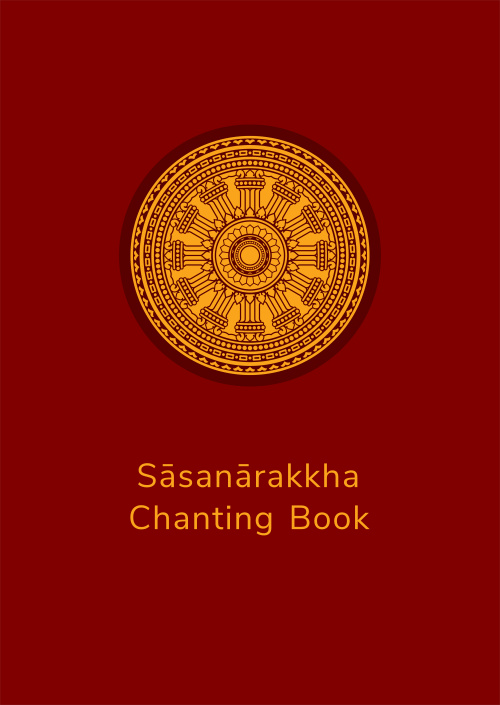
\includegraphics[height=\paperheight]{./desktop-cover.jpg}}
\fi

\pagestyle{empty}
\cleartorecto
\thispagestyle{empty}
\vspace*{5em}

{\centering

\settowidth{\titleLength}{%
  {\Large\chapterTitleFont\textls*{\MakeUppercase{\thetitle}}}%
}

{\Large\chapterTitleFont\textls*{\MakeUppercase{\thetitle}}}\\[0.3\baselineskip]
\setlength{\xheight}{\heightof{X}}
\raisebox{0.5\xheight}{\color[gray]{0.4}\rule{\titleLength}{0.25pt}}\\[0.3\baselineskip]
{\itshape \thesubtitle}

\vfill

\vspace*{5em}

}


\cleartoverso
\thispagestyle{empty}

\vspace*{-\baselineskip}

{%

\fontsize{9}{11}\selectfont
\centering
\setlength{\parindent}{0pt}%
\setlength{\parskip}{0.8\baselineskip}%

% \thetitle\\
% \thesubtitle

This book is offered for free distribution,\\
please do not sell this book.

Download this book in PDF, EPUB and MOBI formats\\
at the following address:

\href{https://sasanarakkha.org/}{sasanarakkha.org}

\vfill

Project Manager: Ā. Ariyadhammika\\
Editors: Ā. Devamitta, Ā. Pāladhammika, Ā. Pamodadhammika\\
Typesetting: Ā. Gambhiro, Ā. Pāladhammika\\
Translators: Ā. Aggacitta, Ā. Bodhi, Ā. Sujāto\\
Endnotes: Ā. Ariyadhammika

\vfill

This version was created on:\\
\today\\
\currenttime

\vfill

This work is licensed under a Creative Commons\\
Attribution-NonCommercial-NoDerivatives 4.0 International~License.

Produced with the \LaTeX\ typesetting system,\\
set in Libertinus Serif.

\theEditionInfo

}

\cleartorecto
\thispagestyle{empty}

{\setlength{\parskip}{10pt}

{\centering\fontsize{20}{25}\selectfont
\textsc{We Wish To Gratefully Acknowledge}
\par}

The Saṅghas of Wat Pah Nanachat (WPN), Amaravati, and Abhayagiri for allowing the use of material from their respective chanting books, the late Ven. Dr. Saddhātissa and Mr. Maurice Walshe for their English translations, as well as Ven. Bhikkhu Bodhi for granting permission to use and slightly adapt his translations. Further contributions are found on the previous page.

\vspace*{1.5\baselineskip}

Additional information on translations, as well as deviations\pagenote{%
  Due to the balanced and inspiring selction of chants, as well as for the sake of
  compatability, the WPN chanting book has served as the basis for the SBS
  chanting book. Over time, suggestions for the inclusion of additional chants, as
  well as occasional improvements of existing translations were incorporated. Such
  changes were meticulously marked down in the endnotes, so that someone familiar
  with the SBS chanting book can straight away find the relevant differences,
  which can be useful when visiting a branch monastery of the Ajahn Chah lineage,
  in order to know in which places to revert to the original version.}
from WPN Chanting Book (2014), have been annotated by Ven. Ariyadhammika in the endnotes.

\bigskip

{\centering
To Āyasmā Aggacitta, the founding father of\\
Sāsanārakkha Buddhist Sanctuary.

\bigskip


\includegraphics[height=65mm]{SBS_logo_Tuck_Loon_BAedit_2020_small.jpg}

}

}

\chapter{Recitation Schedule}
\label{schedule}

{\centering

  {\pdfbookmark[2]{Set 1}{set1}\libertinusFont\selectfont\textbf{\textsc{\fontsize{18}{12}\selectfont\textls*{Set 1}}}}\\

  \textsc{\fontsize{14.4}{28}\selectfont
    \hyperref[buddhas-first-exclamation]{The Buddha's First Exclamation} \ifdesktopversion\else\pageref{buddhas-first-exclamation}\fi\\
    \hyperref[wheel-of-dhamma-abridged]{Setting in Motion the Wheel of Dhamma} \ifdesktopversion\else\pageref{wheel-of-dhamma-abridged}\fi\\
    \hyperref[true-false-refuges]{Going to True and False Refuges} \ifdesktopversion\else\pageref{true-false-refuges}\fi\\
    \hyperref[four-great-references]{The Four Great References} \ifdesktopversion\else\pageref{four-great-references}\fi\\
    \hyperref[patimokkha-exhortation]{The Pāṭimokkha Exhortation} \ifdesktopversion\else\pageref{patimokkha-exhortation}\fi\\
    \hyperref[buddhas-final-instruction]{The Buddha's Final Instruction} \ifdesktopversion\else\pageref{buddhas-final-instruction}\fi\\
    \hyperref[uddissanadhitthana]{Uddissan'ādhiṭṭhāna} \ifdesktopversion\else\pageref{uddissanadhitthana}\fi\\
    \hyperref[closing-homage]{Closing Homage (Pāli-English)} \ifdesktopversion\else\pageref{closing-homage}\fi\\
  }

  \vspace{1.0cm}

  {\pdfbookmark[2]{Set 2}{set2}\libertinusFont\selectfont\textbf{\textsc{\fontsize{18}{12}\selectfont\textls*{Set 2}}}}\\

  \textsc{\fontsize{14.4}{28}\selectfont
    \hyperref[characteristic-of-not-self]{The Discourse on the Characteristic of Not-Self} \ifdesktopversion\else\pageref{characteristic-of-not-self}\fi\\
    \hyperref[fire-sermon]{The Fire Sermon} \ifdesktopversion\else\pageref{fire-sermon}\fi\\
    \hyperref[gradual-training]{The Gradual Training} \ifdesktopversion\else\pageref{gradual-training}\fi\\
    \hyperref[sharing-aspirations]{Sharing and Aspirations} \ifdesktopversion\else\pageref{sharing-aspirations}\fi\\
    \hyperref[closing-homage]{Closing Homage (Pāli-English)} \ifdesktopversion\else\pageref{closing-homage}\fi\\
  }

  \clearpage

  {\pdfbookmark[2]{Set 3}{set3}\libertinusFont\selectfont\textbf{\textsc{\fontsize{18}{12}\selectfont\textls*{Set 3}}}}\\

  \textsc{\fontsize{14.4}{28}\selectfont
    \hyperref[noble-eightfold-path]{The Noble Eightfold Path} \ifdesktopversion\else\pageref{noble-eightfold-path}\fi\\
    \hyperref[repulsiveness-of-food]{The Repulsiveness of Food} \ifdesktopversion\else\pageref{repulsiveness-of-food}\fi\\
    \hyperref[requisites-for-awakening]{Requisites for Awakening} \ifdesktopversion\else\pageref{requisites-for-awakening}\fi\\
    \hyperref[principles-of-non-decline]{Principles of Non-Decline} \ifdesktopversion\else\pageref{principles-of-non-decline}\fi\\
    \hyperref[protection]{On Protection} \ifdesktopversion\else\pageref{protection}\fi\\
    \hyperref[sharing-all-merits]{Sharing of Merits} \ifdesktopversion\else\pageref{sharing-all-merits}\fi\\
    \hyperref[closing-homage]{Closing Homage (Pāli-English)} \ifdesktopversion\else\pageref{closing-homage}\fi\\
  }

  \vspace{1.0cm}

  {\pdfbookmark[2]{Set 4}{set4}\libertinusFont\selectfont\textbf{\textsc{\fontsize{18}{12}\selectfont\textls*{Set 4}}}}\\

  \textsc{\fontsize{14.4}{28}\selectfont
    \hyperref[dedication-of-offerings]{Homage to the Triple Gem} \ifdesktopversion\else\pageref{dedication-of-offerings}\fi\\
    \hyperref[universal-well-being]{Universal Well-Being} \ifdesktopversion\else\pageref{universal-well-being}\fi\\
    \hyperref[seven-factors-of-awakening]{The Seven Factor of Awakening} \ifdesktopversion\else\pageref{seven-factors-of-awakening}\fi\\
    \hyperref[words-on-loving-kindness]{The Buddha's Words on Loving-Kindness} \ifdesktopversion\else\pageref{words-on-loving-kindness}\fi\\
    \hyperref[sharing-merits-departed]{Sharing of Merits with the Departed (Pāli-English)} \ifdesktopversion\else\pageref{sharing-merits-departed}\fi\\
    \hyperref[sharing-merits-devas]{Sharing of Merits with the Devas (Pāli)} \ifdesktopversion\else\pageref{sharing-merits-devas}\fi\\
    \hyperref[closing-homage]{Closing Homage (Pāli-English)} \ifdesktopversion\else\pageref{closing-homage}\fi\\
  }

  \clearpage

  {\pdfbookmark[2]{Set 5}{set5}\libertinusFont\selectfont\textbf{\textsc{\fontsize{18}{12}\selectfont\textls*{Set 5}}}}\\

  \textsc{\fontsize{14.4}{28}\selectfont
    \hyperref[mindfulness-of-breathing]{Mindfulness of Breathing} \ifdesktopversion\else\pageref{mindfulness-of-breathing}\fi\\
    \hyperref[highest-blessings]{The Highest Blessings} \ifdesktopversion\else\pageref{highest-blessings}\fi\\
    \hyperref[three-characteristics]{The Three Characteristics} \ifdesktopversion\else\pageref{three-characteristics}\fi\\
    \hyperref[four-requisites]{The Four Requisites} \ifdesktopversion\else\pageref{four-requisites}\fi\\
    \hyperref[five-reflections]{Five Subjects for Frequent Reflection} \ifdesktopversion\else\pageref{five-reflections}\fi\\
    \hyperref[32-parts]{The Thirty-Two Body Parts} \ifdesktopversion\else\pageref{32-parts}\fi\\
    \hyperref[principles-of-cordiality]{Principles of Cordiality} \ifdesktopversion\else\pageref{principles-of-cordiality}\fi\\
    \hyperref[highest-honour-aspirations]{The Highest Honour and Aspirations} \ifdesktopversion\else\pageref{highest-honour-aspirations}\fi\\
    \hyperref[closing-homage]{Closing Homage (Pāli-English)} \ifdesktopversion\else\pageref{closing-homage}\fi\\
  }

  \vspace{1.0cm}

  {\pdfbookmark[2]{Set 6}{set6}\libertinusFont\selectfont\textbf{\textsc{\fontsize{18}{12}\selectfont\textls*{Set 6}}}}\\

  \textsc{\fontsize{14.4}{28}\selectfont
    \hyperref[anatta-lakkhana]{Anatta-lakkhaṇa Sutta} \ifdesktopversion\else\pageref{anatta-lakkhana}\fi\\
    \hyperref[striving-according-to-dhamma]{Striving According to the Dhamma} \ifdesktopversion\else\pageref{striving-according-to-dhamma}\fi\\
    \hyperref[divine-abidings]{The Divine Abidings} \ifdesktopversion\else\pageref{divine-abidings}\fi\\
    \hyperref[ten-reflections]{Ten Subjects for Frequent Reflection\\ \vspace{-0.4cm} by One Gone Forth} \ifdesktopversion\else\pageref{ten-reflections}\fi\\
    \hyperref[sharing-aspirations]{Sharing and Aspirations} \ifdesktopversion\else\pageref{sharing-aspirations}\fi\\
    \hyperref[closing-homage]{Closing Homage (Pāli-English)} \ifdesktopversion\else\pageref{closing-homage}\fi\\
  }

  \clearpage

  {\pdfbookmark[2]{Set 7}{set7}\libertinusFont\selectfont\textbf{\textsc{\fontsize{18}{12}\selectfont\textls*{Set 7}}}}\\

  \textsc{\fontsize{14.4}{28}\selectfont
    \hyperref[dependent-origination]{Dependent Origination} \ifdesktopversion\else\pageref{dependent-origination}\fi\\
    \hyperref[dhamma-in-brief]{The Dhamma in Brief} \ifdesktopversion\else\pageref{dhamma-in-brief}\fi\\
    \hyperref[uddissanadhitthana]{Uddissan'ādhiṭṭhāna} \ifdesktopversion\else\pageref{uddissanadhitthana}\fi\\
    \hyperref[closing-homage]{Closing Homage (Pāli-English)} \ifdesktopversion\else\pageref{closing-homage}\fi\\
  }

  \vspace{1.0cm}

  {\pdfbookmark[2]{Set 8}{set8}\libertinusFont\selectfont\textbf{\textsc{\fontsize{18}{12}\selectfont\textls*{Set 8}}}}\\

  \textsc{\fontsize{14.4}{28}\selectfont
    \hyperref[aditta-pariyaya]{Āditta-Pariyāya Sutta} \ifdesktopversion\else\pageref{aditta-pariyaya}\fi\\
    \hyperref[burdens]{The Burdens} \ifdesktopversion\else\pageref{burdens}\fi\\
    \hyperref[respect-for-the-dhamma]{Respect for the Dhamma} \ifdesktopversion\else\pageref{respect-for-the-dhamma}\fi\\
    \hyperref[single-excellent-night]{A Single Excellent Night} \ifdesktopversion\else\pageref{single-excellent-night}\fi\\
    \hyperref[ratthapala]{From the Elder Raṭṭhapāla}  \ifdesktopversion\else\pageref{ratthapala}\fi\\
    \hyperref[parapariya]{From the Elder Pārāpariya} \ifdesktopversion\else\pageref{parapariya}\fi\\
    \hyperref[misc-verses]{Miscellaneous Verses} \ifdesktopversion\else\pageref{misc-verses}\fi\\
    \hyperref[highest-honour-aspirations]{The Highest Honour and Aspirations} \ifdesktopversion\else\pageref{highest-honour-aspirations}\fi\\
    \hyperref[closing-homage]{Closing Homage (Pāli-English)} \ifdesktopversion\else\pageref{closing-homage}\fi\\
  }

  \clearpage

  {\pdfbookmark[2]{Set 9}{set9}\libertinusFont\selectfont\textbf{\textsc{\fontsize{18}{12}\selectfont\textls*{Set 9}}}}\\

  \textsc{\fontsize{14.4}{28}\selectfont
    \hyperref[deva-aradhana]{Protective Recitations (Pāli)} \ifdesktopversion\else\pageref{deva-aradhana}\fi\\
    \hyperref[sharing-merits-departed]{Sharing of Merits with the Departed (Pāli)} \ifdesktopversion\else\pageref{sharing-merits-departed}\fi\\
    \hyperref[sharing-merits-devas]{Sharing of Merits with the Devas (Pāli)} \ifdesktopversion\else\pageref{sharing-merits-devas}\fi\\
    \hyperref[closing-homage]{Closing Homage (Pāli)} \ifdesktopversion\else\pageref{closing-homage}\fi\\
  }

  \vspace{1.0cm}

  {\pdfbookmark[2]{Set 10}{set10}\libertinusFont\selectfont\textbf{\textsc{\fontsize{18}{12}\selectfont\textls*{Set 10}}}}\\

  \textsc{\fontsize{14.4}{28}\selectfont
    \hyperref[pubba-bhaga-nama-kara-patho-funeral]{Funeral Recitations (Pāli)} \ifdesktopversion\else\pageref{pubba-bhaga-nama-kara-patho-funeral}\fi\\
    \hyperref[recollection-of-impermanence]{Recollection of Impermanence} \ifdesktopversion\else\pageref{recollection-of-impermanence}\fi\\
    \hyperref[yatha-vari-vaha-pura]{Thanksgiving Recitations (Pāli)} \ifdesktopversion\else\pageref{yatha-vari-vaha-pura}\fi\\
    \hyperref[just-as-rivers]{Just as Rivers} \ifdesktopversion\else\pageref{just-as-rivers}\fi\\
    \hyperref[sharing-all-merits]{Sharing of All Merits} \ifdesktopversion\else\pageref{sharing-all-merits}\fi\\
    \hyperref[closing-homage]{Closing Homage (Pāli-English)} \ifdesktopversion\else\pageref{closing-homage}\fi\\
  }}

% \section{The Purpose and Benefits of Dhamma Recitation}
\chapter[The Purpose and Benefits of Dhamma Recitation]{The Purpose and Benefits \\ of Dhamma Recitation}
% % TODO: remove bars here and and line break after Benefits
\label{purpose-and-benefits}

\subsection*{Historical Background}

After finding the path to \textit{Nibbāna} and some initial hesitation, the Buddha eventually decided to teach the Dhamma (MN 26). His first disciples were a group of five monks, and with the awakening of one of them, Ven. Kondañña, the wheel of Dhamma was set in motion (SN 56.11). While these first disciples were taught exclusively by the Buddha himself, soon afterwards more monks reached the final goal. Subsequently, the Buddha sent out the first sixty arahants to teach the Dhamma (SN 4.5, Vin I 20).\\

During that period of ancient India, religious texts were not commonly written down. Even for ordinary education purposes, much of learning happened through memorization. Writing was known, but not used for religious texts, which were considered too sacred to be put into writing; instead they were meant to live in the minds and hearts of those who saw their value, and made the effort to memorize them. In particular, the Brahmins were known for their proficiency in committing their corpus of sacred texts (\textit{Vedas}) to memory and maintaining them with astonishing accuracy. Part of their skill was because memorization started from a young age. Likewise, also among Buddhist literature we can discover clear traces of standardization and mnemonic tools, meant to aim at precision and ease of memorization. In particular, the use of recurring stock phrases makes it easier to commit a large corpus of texts to memory (Anālayo, 2019). There is not much known about the specific teachings shared with their audience by the first arahants who went out to teach the Dhamma. But it is fair to assume that they took some teachings with them that were quick and easy to memorize. Let us also keep in mind that the Buddha’s disciples were not trained in memorization from childhood, but they came from all walks of life – young, old, educated, uneducated etc. Only when the Saṅgha had grown in size, monks who specialized in recitation travelled all across India and shared the Buddha’s teachings with those eager to hear them (Analayo, 2007).\\

A passage that illustrates the Buddha’s own appreciation of recitation, stems from a conversation he had with a monk who had gone forth just recently. Without warning, the Buddha asked him to recite the Dhamma. The newly ordained monk recited the \textit{Aṭṭhakavagga} of \textit{Sutta Nipāta} (Ud 5.6). The Buddha was pleased and complimented the monk on his skills in remembering, keeping in mind, articulating, and enunciating of the texts. This highlights the Buddha’s emphasis that recitation of the Dhamma was meant to be taken seriously by his ordained disciples.\\

\subsection*{The Workings of Memory}

Contrary to our intuition, memory doesn’t function like a scanner or copying machine that takes a snapshot of a text or event, and saves it for later. Instead, anecdotal memory works in a relational manner. The brain links new information that comes in through any of the 6 senses to concepts based on memories from the past. We understand new things in the light of and from the perspective of, things we already know. Likewise, we “remember” old things through the filters and biases of the present moment. “It is so natural for us to draw inferences that we are often unaware that we are doing so” (Eysenck, 1992/2005). This interplay between past and present gives our memory great potential due to its seemingly unlimited storage capacity (the Buddha recollected past lifetimes from memory, counting back many eons of world-dissolution and evolution). At the same time the interplay between past and future also makes memory inherently unreliable. The importance of memorization becomes clear. When texts are memorized literally, personal interpretation, biases, and coloring by past experiences and present circumstances have less opportunity to distort the information. Accuracy increases further if one checks the memorized text from time to time against its original, either by looking it up in a book, or by reciting it together with others. In this way, differences become apparent straight away.\\

\subsection*{Benefits for Dhamma Practice}

In the discourses the Buddha is often depicted taking up the topic of recitation when explaining to monks the proper way to learn the teachings, and make these teachings the vessel within which their own wisdom can grow.\\

\begin{quote}
  “He has learned much, remembers what he has learned, and accumulates what he has learned. Those teachings that are good in the beginning, good in the middle, and good in the end, with the right meaning and phrasing, which proclaim the perfectly complete and pure spiritual life—such teachings as these he has learned much of, retained in mind, recited verbally, mentally investigated, and penetrated well by view. This is the fifth cause and condition that leads to obtaining the wisdom fundamental to the spiritual life.” (AN 8.2)\\
\end{quote}

% TODO: should we use suttaRef here too?

In our current age of easy access to Dhamma books and multimedia, it is tempting to conclude that it is now not necessary anymore to memorize large bodies of texts for the sake of transmission, and that we are blessed with being able to read any of the texts at any time, from the comfort of our kuṭis or living rooms. And blessed we are. Nonetheless, even today recitation has benefits that surpass a regular silent reading, or even reading out loud. As seen in the earlier quote from AN 8.2, the Buddha doesn’t only speak about reciting the texts verbally, but also about retaining them in mind and investigating them mentally. This is where the benefits of recitation differ considerably from a more casual reading, or even from chanting with the help of a chanting book. By means of committing a text to memory, it lives much deeper within our minds and hearts, and we can reflect on it whenever and wherever. Dhamma that has been well-memorized, is always with us. The Buddha’s teachings become accessible in the very moment we need them, without having to resort to a book or an e-reader.\\

Since right view is the first of eight path factors, it is of great importance for progress on the path to keep the Buddha’s teachings in mind, so that they can shape our views and perspectives; keeping them in memory in such a way that one can recognize their relevance whenever a situation in life occurs when they naturally manifest, or when they are most necessary to intentionally recall. Recollecting the Dhamma can be a source of joy, leading to rapture, tranquility, and concentration (AN 5.26); factors that can lead to a pleasant abiding here and now. It can also help to abandon drowsiness (AN 7.61), as well as speed up recovery from illness (AN 46.16), or to achieve a stage of awakening even on the deathbed (AN 6.56). In fact, reciting the Dhamma is one of the occasions that can even bring about the attainment of final liberation (AN 5.26).\\

\begin{quote}
  Though the bhikkhu Phagguṇa’s mind had not yet been liberated from the five lower fetters, when he heard that discourse on the Dhamma, his mind was liberated from them… There are, Ānanda, these six benefits of listening to the Dhamma at the proper time and of examining the meaning at the proper time. What six?\\

  …At the time of his death he does not get to see the Tathāgata or a disciple of the Tathāgata, but he ponders, examines, and mentally inspects the Dhamma as he has heard it and learned it. As he does so, his mind is liberated in the unsurpassed extinction of the acquisitions. This is the sixth benefit of examining the meaning at the proper time. (AN 6.56)\\

  In whatever way the bhikkhu recites the Dhamma in detail as he has heard it and learned it, in just that way, in relation to that Dhamma, he experiences inspiration in the meaning and inspiration in the Dhamma. As he does so, joy arises in him. When he is joyful, rapture arises. For one with a rapturous mind, the body becomes tranquil. One tranquil in body feels pleasure. For one feeling pleasure, the mind becomes concentrated. This is the third basis of liberation, by means of which, if a bhikkhu dwells heedful, ardent, and resolute, his unliberated mind is liberated, his undestroyed taints are utterly destroyed, and he reaches the as-yet-unreached unsurpassed security from bondage. (AN 5.26)\\
\end{quote}

\subsection*{Benefits for Rebirth}

The depth to which a mere reading of a text penetrates the mind is incomparable to the depth of penetration that can be reached by memorization. AN 4.191 depicts monks who have memorized the Dhamma, and are subsequently reborn in circumstances with little to no exposure to the Dhamma. The sutta explains that not only in the current lifetime, but also in lifetimes ahead, the Dhamma that was previously memorized will be accessible and has a chance of being re-cognized or recollected even in a future existence e.g. as a deva. With the support of sufficient samādhi, not only can the Dhamma be recollected, but even one’s past lives:\\

\begin{quote}
  “Bhikkhus, …there are things to be realized by memory… And what are the things to be realized by memory? One’s past abodes are to be realized by memory. “ (AN 4.189)\\
\end{quote}

\subsection*{Benefits for Communal Life}

Besides being of benefit to one’s own Dhamma practice, and the benefits during future lifetimes, reciting the Dhamma can also have a beneficial impact on communal life. Accounts of the Buddhist councils (\textit{saṅgīti}; lit. recitations) show that in all these important events of Buddhist history when the extended Saṅgha family came together, the DhammaVinaya was recited together, as a means to remain aligned with the teachings and to foster harmony. Another feature of monastic communities, is the fortnightly recitation of the \textit{Pātimokkha}, the rules for monks and nuns, in which even solitary forest dwellers, including Arahants, were encouraged by the Buddha to participate, as they make their way to the nearest monastery in the vicinity (Mv.II.5.5). Recitation of texts together, not only strengthens a common commitment to the DhammaVinaya, but in a more practical way, it also enables monastics to chant in sync and unison when reciting together with their spiritual companions. This not only increases clarity and understanding, but also makes for a more homogenous listening experience at a ceremony, e.g. a dāna or bereavement service conducted by monastics. Furthermore, the coming together frequently to recite the Buddha’s teachings, creates a bond among Saṅgha members and leads to their growth. This would not be so if everyone recites the Dhamma on his own.\\

\begin{quote}
  And what, bhikkhus, are the seven principles of non-decline? (1) “As long as the bhikkhus assemble often and hold frequent assemblies, only growth is to be expected for them, not decline. (2) “As long as the bhikkhus assemble in harmony, adjourn in harmony, and conduct the affairs of the Saṅgha in harmony, only growth is to be expected for them, not decline. (AN 7.23)\\
\end{quote}

\subsection*{Recitation Among Monastics}

While it is not uncommon in our current time and age that teachers share the Dhamma without any reference to the Buddha or his teachings, in the Buddha’s time the teachings were passed on from teacher to disciple by means of recitation. The Vinaya texts explain that \textit{“if the preceptor wants one to recite [C: memorize passages of Dhamma or Vinaya], one should recite. If he wants to interrogate one [C: on the meaning of the passages], one should answer his interrogation."} (Cv.VIII.12.2-11)\\

BMC I mentions that the \textit{Vibhaṅga} to \textit{Pācittiya} 4 lists four ways in which a person might be trained to be a reciter of a text:

\begin{enumerate}
  \item The teacher and student recite in unison, i.e. beginning together and ending together.
  \item The teacher begins a line, the student joins in, and they end together.
  \item The teacher recites the beginning syllable of a line together with the student, who then completes it alone.
  \item The teacher recites one line, and the student recites the next line alone.
\end{enumerate}

In order for a monk to be free from dependence (\textit{nissaya}) on a teacher, \textit{“he must be learned and intelligent, knowing both Pāṭimokkhas … and must have been ordained as a bhikkhu for at least five years”} (Mv.I.53.5-13).\\

\clearpage

The Commentary says that a learned bhikkhu must have memorized:

\begin{itemize}
  \item Both \textit{Pātimokkhas} (for the \textit{bhikkhus} and \textit{bhikkhunīs}).
  \item The Four \textit{Bhāṇavāras} — a set of auspicious chants that are still regularly memorized in Sri Lanka as the \textit{Mahā-pirit poṭha}.
  \item A discourse that is helpful as a guide for sermon-giving.
  \item Three kinds of \textit{anumodanā} (rejoicing in the merit of others) chants: for meals; for auspicious merit-making ceremonies, such as blessing a house; and for non-auspicious ceremonies, i.e. any relating to a death.
\end{itemize}

Lastly, when monastics from other sects wanted to become monks in the Buddha’s dispensation, they typically had to undergo a four-month probation period. However, \textit{“a probationer fails in his probation and is not to be accepted … if he does not have a keen desire for recitation.”} (Mv.I.38.5-10)\\

Once again, we can see the immense emphasis that was placed on memorization and recitation, starting already during the Buddha’s own ministry, and having continued all the way to the 21st century, where we can still find monks who are able to memorize the entirety of the \textit{Tipiṭaka}.\\

\subsection*{What to Recite}

While recitation and memorization of the Dhamma yields several benefits, and one may be committed to dedicate some amount of time to this worthwhile endeavor, one important task remains. Given the limited amount of texts one may be able to memorize and maintain in memory, the task is: the selection of texts for recitation and memorization, there being such a vast amount of teachings that the Buddha left behind. What is essential - what is secondary? Once again, we are in the fortunate situation that the Buddha himself gave guidance in what he regarded as the core teachings. In MN 104 the Buddha points to a set of 37 teachings, commonly known as the “Wings of Awakening” (\textit{bodhipakkhiyā dhammā}). Included in these 37 Dhammas are the four foundations of mindfulness, the four right strivings, the four bases of spiritual power, the five faculties, the five powers, the seven factors of awakening, and the noble eightfold path. (DN 16). Other teachings that are commonly held in high esteem are the Discourse on Setting in Motion the Wheel of Dhamma (\textit{Dhammacakkappavattanasutta}), the Gradual Training, and The Dhamma in Brief. All of these are teachings that can help the earnest practitioner to gain an overview of the Dhamma and one’s path to liberation. Practicing accordingly, further recollection and recitation of such teachings also helps to correctly assess one’s own progress on the path.\\

Besides these general teachings, the Buddha also went into great depth in explaining the most profound doctrines, some of which are related to the conceptual framework surrounding the practice, while others are directly related to formal meditation. Early sermons that stand out in this context are the Discourse on the Characteristics of Not-Self (\textit{Anatta-lakkhaṇa Sutta}), the Fire Sermon (\textit{Āditta-Pariyāya Sutta}), the Buddha’s First and Final Words, Mindfulness of Breathing, and Dependent Origination. All of these are profound, deep teachings that highlight key aspects of the path to awakening. These are teachings that are good to memorize and recite again and again (AN 10.48), allowing their deep meaning to gradually seep into our hearts.\\

From these profound teachings we can take a step back to the practical, day-to-day perceptions that the Buddha specifically recommended to be frequently reflected upon. In this category we find the 5 and 10 Subjects for Frequent Recollection, also the Reflections on The Four Requisites, and a separate reflection on The Repulsiveness of Food. Recollection of Impermanence, The 3 Characteristics, and The Thirty-Two Body Parts are also frequently mentioned in the discourses. Perceptions that are closely related to the 2nd path factor of the noble eightfold path, i.e. right thought (\textit{sammā saṇkappa}), are the Mettasutta and The Divine Abidings. Perceptions that arouse the four \textit{Brahmavihāras} can seamlessly lead the practitioner towards the 8th path factor, \textit{sammā samādhi}. At times when energy is lacking, however, chants that inspire, motivate, or arouse urgency, can be used to heat up and revitalize the practice. This is where Striving According to the Dhamma, The Burdens, Respect for the Dhamma, and the Miscellaneous Verses can come to the rescue.\\

Lastly, this Recitation Book also includes passages that illuminate how to establish good relations among fellow practitioners, such as the Principles of Cordiality, Principles of Non-Decline, and The Four Great References. Also included are chants that monks commonly perform as services to the laity, such as Anumodanā, Sharing of Merits, and Funeral Chants.\\

To summarize, memorization of the Dhamma and group recitation fulfill a variety of different purposes and benefits, ranging all the way from the mundane aspects such as the ability to recite in unison, the fostering of communal harmony, all the way to the attainment of final liberation.\\

\subsection*{How to Recite}

See chapter “Pāli Phonetics \& Pronunciation” in the Appendix\\

\subsection*{Sources}
Oral Dimensions of Pāli Discourses: Periscopes, other Mnemonic Techniques and the Oral Performance Context, Analayo, Canadian Journal of Buddhist Studies, 2007-3\\
\\
Ancient Indian Education and Mindfulness, Anālayo, Springer Science+Business Media, 2019\\
\\
Cognitive Psychology, Hove: Psychology Press, Eysenck, M. W. et al., 1992/2005\\
\\
The Buddhist Monastic Code II, Ṭhānissaro Bhikkhu, Metta Forest Monastery, 2013


\cleartorecto
\pagestyle{toponerow-frontmatter}
\chapterstyle{adrasteia-toc}

\tableofcontents*

\chapterstyle{adrasteia-frontmatter}

\mainmatter
\pagestyle{toponerow}

\cleartorecto
\part{Pāli-English Recitations}

{\raggedright
  \chapterOpeningPage{morning-chanting.pdf}

\chapter{Homage to the Triple Gem}

\section{Dedication of Offerings}
\label{dedication-of-offerings}

[Yo so] bhagavā arahaṁ sammāsambuddho

\begin{english-hang}
  To the Blessed One the Worthy One\label{hl-1}\pagenote{%
    Orig: ``The Lord''. The underlying Pāli term is ``\textit{Arahant}''. ``Lord'',
    however, has connotations that do not fit well to the way the Buddha is
    portrayed in the discourses. In dictionaries ``lord'' is commonly defined
    as: \emph{``an appellation for a person or deity who has authority, control, or
      power over others, acting like a master, a chief, or a ruler.'' The ``Worthy
      One'' seems a better choice of terms, since it is also how ``Arahant'' was
      used in pre-Buddhist era. PTS explains: ``[Vedic arhant, ppr. of arhati
      (see arahati), meaning deserving, worthy] . Before Buddhism used as
      honourific title of high officials like the English "His Worship" ; at the
      rise of Buddhism applied popularly to all ascetics (Dial. III.3–6).''}
    Throughout this chanting book, all occurrences of ``\textit{Arahant}'' have
    therefore been consistently translated as ``Worthy One'', thus substituting
    previous translations as ``The Lord'', ``Noble One'' etc. \hyperref[hl-1]{Back}}
  who fully attained Perfect Enlightenment
\end{english-hang}

Svākkhāto yena bhagavatā dhammo

\begin{english}
  To the Teaching which he expounded so well
\end{english}

Supaṭipanno yassa bhagavato sāvakasaṅgho

\begin{english}
  And to the Blessed One's disciples who have practiced well
\end{english}

Tam-mayaṁ bhagavantaṁ sadhammaṁ sasaṅghaṁ

\begin{english}
  To these the Buddha the Dhamma and the Saṅgha
\end{english}

Imehi sakkārehi yathārahaṁ āropitehi abhipūjayāma

\begin{english}
  We render with offerings our rightful homage
\end{english}

Sādhu no bhante bhagavā sucira-parinibbutopi

\begin{english}
  It is well for us that the Blessed One\\
  Having attained liberation
\end{english}

Pacchimā-janatānukampa-mānasā

\begin{english}
  Still had compassion for later generations
\end{english}

Ime sakkāre duggata-paṇṇākāra-bhūte paṭiggaṇhātu

\begin{english}
  May these simple offerings be accepted
\end{english}

Amhākaṁ dīgharattaṁ hitāya sukhāya

\begin{english}
  For our long-lasting benefit and for the happiness it gives us
\end{english}

Arahaṁ sammāsambuddho bhagavā

\begin{english}
  The Worthy One the Perfectly Enlightened and Blessed One
\end{english}

Buddhaṁ bhagavantaṁ abhivādemi\relax

\begin{english}
  I render homage to the Buddha the Blessed One \hfill{(Bow)}
\end{english}

[Svākkhāto] bhagavatā dhammo

\begin{english}
  The Teaching so completely explained by him
\end{english}

Dhammaṁ namassāmi\relax

\begin{english}
  I bow to the Dhamma \hfill{(Bow)}
\end{english}

[Supaṭipanno] bhagavato sāvakasaṅgho

\begin{english}
  The Blessed One's disciples who have practiced well
\end{english}

Saṅghaṁ namāmi

\begin{english}
  I bow to the Saṅgha \hfill{(Bow)}
\end{english}

\section{Preliminary Homage}
\label{preliminary-homage}

\begin{leader}
  〈 Handa mayaṁ buddhassa bhagavato pubbabhāga-namakāraṁ karomase 〉
\end{leader}

\begin{leader-english}
  〈 Now let us pay preliminary homage to the Buddha 〉
\end{leader-english}

Namo tassa bhagavato arahato sammāsambuddhassa \hfill{[3x]}

\begin{english}
  Homage to the Blessed Worthy and Perfectly Enlightened One \hfill{[3x]}
\end{english}

\section{Homage to the Buddha}
\label{homage-buddha}

\begin{leader}
  〈 Handa mayaṁ buddhābhitthutiṁ karomase 〉
\end{leader}
\begin{leader-english}
  〈 Now let us recite in praise of the Buddha 〉
\end{leader-english}

Yo so tathāgato arahaṁ sammāsambuddho

\begin{english}
  The Tathāgata is the Worthy One the Perfectly Enlightened One
\end{english}

Vijjācaraṇa-sampanno

\begin{english}
  He is impeccable in conduct and understanding
\end{english}

Sugato

\begin{english}
  The Accomplished One
\end{english}

Lokavidū

\begin{english}
  The Knower of the Worlds
\end{english}

Anuttaro purisadamma-sārathi

\begin{english}
  Unsurpassed leader of persons to be tamed\pagenote{%
    Orig: ``He trains perfectly those who wish to be trained''. The aspect of wishing to be trained is not found in the Pāli.}
\end{english}

Satthā deva-manussānaṁ

\begin{english}
  He is teacher of gods and humans
\end{english}

Buddho bhagavā

\begin{english}
  He is awake and holy
\end{english}

Yo imaṁ lokaṁ sadevakaṁ samārakaṁ sabrahmakaṁ

\begin{english}
  In this world with its gods ̓ demons and kind spirits
\end{english}

\begin{pali-hang}
  Sassamaṇa-brāhmaṇiṁ pajaṁ sadeva-manussaṁ sayaṁ abhiññā sacchikatvā pavedesi
\end{pali-hang}

\begin{english}
  Its seekers and sages \breathmark\ celestial and human beings\\
  He has by deep insight revealed the truth
\end{english}

\begin{pali-hang}
Yo dhammaṁ desesi ādi-kalyāṇaṁ majjhe-kalyāṇaṁ pariyosāna-kalyāṇaṁ
\end{pali-hang}

\begin{english}
  He has pointed out the Dhamma\\
  Beautiful in the beginning\\
  Beautiful in the middle\\
  Beautiful in the end\\
\end{english}

\begin{pali-hang}
Sātthaṁ sabyañjanaṁ kevala-paripuṇṇaṁ parisuddhaṁ brahma-cariyaṁ pakāsesi
\end{pali-hang}

\begin{english}
  He has explained the holy life of complete purity\pagenote{%
    Orig: ``He has explained the spiritual life of complete purity''. While ``spiritual life'' is not a bad translation, for the sake of consistency with the rest of the chanting book, this occurrence was changed to ``holy life''}\\
  In its essence and conventions
\end{english}

\begin{pali-hang}
Tam-ahaṁ bhagavantaṁ abhipūjayāmi tam-ahaṁ bhagavantaṁ sirasā namāmi
\end{pali-hang}

\begin{english}
  I chant my praise to the Blessed One\\
  I bow my head to the Blessed One \hfill{(Bow)}
\end{english}

\section{Homage to the Dhamma}
\label{homage-dhamma}

\begin{leader}
  〈 Handa mayaṁ dhammābhitthutiṁ karomase 〉
\end{leader}
\begin{leader-english}
  〈 Now let us recite in praise of the Dhamma 〉
\end{leader-english}

Yo so svākkhāto bhagavatā dhammo

\begin{english}
  The Dhamma is well-expounded by the Blessed One
\end{english}

Sandiṭṭhiko

\begin{english}
  Apparent here and now
\end{english}

Akāliko

\begin{english}
  Timeless
\end{english}

Ehipassiko

\begin{english}
  Encouraging investigation
\end{english}

Opanayiko

\begin{english}
  Leading inwards
\end{english}

Paccattaṁ veditabbo viññūhi

\begin{english}
  To be experienced individually by the wise
\end{english}

\begin{pali-hang}
Tam-ahaṁ dhammaṁ abhipūjayāmi tam-ahaṁ dhammaṁ sirasā namāmi
\end{pali-hang}

\begin{english}
  I chant my praise to this teaching\\
  I bow my head to this truth \hfill{(Bow)}
\end{english}

\section{Homage to the Saṅgha}
\label{homage-sangha}

\begin{leader}
  〈 Handa mayaṁ saṅghābhitthutiṁ karomase 〉
\end{leader}
\begin{leader-english}
  〈 Now let us recite in praise of the Saṅgha 〉
\end{leader-english}

Yo so supaṭipanno bhagavato sāvakasaṅgho

\begin{english}
  They are the Blessed One's disciples who have practiced well
\end{english}

Ujupaṭipanno bhagavato sāvakasaṅgho

\begin{english}
  Who have practiced directly\pagenote{%
    To practice ``directly''(Pāli: \textit{uju}) means, to practice the most direct way to \textit{nibbāna}; the straight way; no B-tours.}
\end{english}

Ñāyapaṭipanno bhagavato sāvakasaṅgho\pagenote{%
  Orig: ``Who have practiced insightfully''}

\begin{english}
  Who have practiced correctly\pagenote{%
    Orig: ``Those who practice with integrity''}
\end{english}

Sāmīcipaṭipanno bhagavato sāvakasaṅgho

\begin{english}
  Who have practiced properlyi
\end{english}

Yadidaṁ cattāri purisayugāni aṭṭha purisapuggalā

\begin{english}
  That is the four pairs the eight kinds of Noble Beings
\end{english}

Esa bhagavato sāvakasaṅgho

\begin{english}
  These are the Blessed One's disciples
\end{english}

Āhuneyyo

\begin{english}
  Such ones are worthy of gifts
\end{english}

Pāhuneyyo

\begin{english}
  Worthy of hospitality
\end{english}

Dakkhiṇeyyo

\begin{english}
  Worthy of offerings
\end{english}

Añjali-karaṇīyo

\begin{english}
  Worthy of respect
\end{english}

Anuttaraṁ puññakkhettaṁ lokassa

\begin{english}
  They give occasion for incomparable goodness to arise in the world
\end{english}

\begin{pali-hang}
  Tam-ahaṁ saṅghaṁ abhipūjayāmi tam-ahaṁ saṅghaṁ sirasā namāmi
\end{pali-hang}

\begin{english}
  I chant my praise to this Saṅgha\\
  I bow my head to this Saṅgha \hfill{(Bow)}
\end{english}

\section{Salutation to the Triple Gem}
\label{salutation}

\begin{leader}
  〈 Handa mayaṁ ratanattaya-paṇāma-gāthāyo c'eva saṁvega-parikittana-pāṭhañca 〉
\end{leader}
\begin{leader-english}
  〈 Now let us recite our salutation to the Triple Gem and a passage to arouse urgency 〉
\end{leader-english}

Buddho susuddho karuṇā-mahaṇṇavo

\begin{english}
  The Buddha absolutely pure with ocean-like compassion
\end{english}

Yo'ccanta-suddhabbara-ñāṇa-locano

\begin{english}
  Possessing the clear sight of wisdom
\end{english}

Lokassa pāpūpakilesa-ghātako

\begin{english}
  Destroyer of worldly self-corruption
\end{english}

Vandāmi buddhaṁ aham-ādarena taṁ

\begin{english}
  Devotedly indeed \breathmark\ that Buddha I revere
\end{english}

Dhammo padīpo viya tassa satthuno

\begin{english}
  The Teaching of the Lord is like a lamp\pagenote{%
    Orig: ``The teaching of the Lord like a lamp''}
\end{english}

Yo magga-pākāmata-bheda-bhinnako

\begin{english}
  Divided into path and its fruit \breathmark\ the Deathless\pagenote{%
    Orig: ``Illuminating the path and its fruit, the Deathless''}
\end{english}

Lokuttaro yo ca tad-attha-dīpano

\begin{english-hang}
  And illuminating that goal \breathmark\ which is beyond the conditioned world\pagenote{%
    Orig: ``That which is beyond the conditioned world''}
\end{english-hang}

Vandāmi dhammaṁ aham-ādarena taṁ

\begin{english}
  Devotedly indeed \breathmark\ that Dhamma I revere
\end{english}

Saṅgho sukhettābhyati-khetta-saññito

\begin{english}
  The Saṅgha the most fertile ground for cultivation
\end{english}

Yo diṭṭha-santo sugatānubodhako

\begin{english}
  Those who have realised peace\\
  Awakened after the Accomplished One
\end{english}

Lolappahīno ariyo sumedhaso

\begin{english}
  Noble and wise \breathmark\ all longing abandoned
\end{english}

Vandāmi saṅghaṁ aham-ādarena taṁ

\begin{english}
  Devotedly indeed \breathmark\ that Saṅgha I revere
\end{english}

\begin{pali-hang}
  Iccevam-ekantabhipūja-neyyakaṁ vatthuttayaṁ vandayatābhisaṅkhataṁ
\end{pali-hang}

\begin{english}
  This salutation should be made\\
  To that triad\pagenote{%
    Orig: ``To that which is worthy''. This passage refers to the triple (\textit{taya}) gems and not just to the Saṅgha.}
  which is worthy
\end{english}

Puññaṁ mayā yaṁ mama sabbupaddavā

\begin{english}
  Through the power of such good action
\end{english}

Mā hontu ve tassa pabhāva-siddhiyā

\begin{english}
  May all obstacles disappear
\end{english}

Idha tathāgato loke uppanno arahaṁ sammāsambuddho

\begin{english}
  One who knows things as they are \breathmark\ has arisen in this world\pagenote{%
    ``One who knows things as they are'' is an unusual translation for \textit{Tathāgata}. Also ``arisen in'' is better than ``has come into'', otherwise one might think that he has come from somewhere, already being a \textit{Tathāgata}.}\\
  And he is an \textit{Arahant} \breathmark\ a perfectly awakened being
\end{english}

\begin{pali-hang}
  Dhammo ca desito niyyāniko upasamiko parinibbāniko sambodhagāmī sugatappavedito
\end{pali-hang}

\begin{english}
  Teaching the way leading out of delusion\pagenote{%
    No mention of ``delusion'' in the Pāli. It could also refer to \textit{samsāra} or \textit{dukkha}.}\\
  Calming and directing to perfect peace\\
  And leading to enlightenment\\
  This way he has made known\\
\end{english}

Mayan-taṁ dhammaṁ sutvā evaṁ jānāma

\begin{english}
  Having heard the Teaching we know this
\end{english}

Jātipi dukkhā

\begin{english}
  Birth is dukkha
\end{english}

Jarāpi dukkhā

\begin{english}
  Ageing is dukkha
\end{english}

Maraṇampi dukkhaṁ

\begin{english}
  And death is dukkha
\end{english}

Soka-parideva-dukkha-domanass'upāyāsāpi dukkhā

\begin{english}
  Sorrow lamentation pain displeasure\pagenote{%
    Orig: ``grief''}
  and despair are dukkha
\end{english}

Appiyehi sampayogo dukkho

\begin{english}
  Association with the disliked is dukkha
\end{english}

Piyehi vippayogo dukkho

\begin{english}
  Separation from the liked is dukkha
\end{english}

Yamp'icchaṁ na labhati tampi dukkhaṁ

\begin{english}
  Not attaining one's wishes is dukkha
\end{english}

Saṅkhittena pañcupādānakkhandhā dukkhā

\begin{english}
  In brief \breathmark\ the five aggregates of clinging are dukkha\pagenote{%
    Orig: ``In brief the five focuses of identity are dukkha''}
\end{english}

Seyyathīdaṁ

\begin{english}
  These are as follows
\end{english}

Rūpūpādānakkhandho

\begin{english}
  Attachment to form
\end{english}

Vedanūpādānakkhandho

\begin{english}
  Attachment to feeling
\end{english}

Saññūpādānakkhandho

\begin{english}
  Attachment to perception
\end{english}

Saṅkhārūpādānakkhandho

\begin{english}
  Attachment to volitional formations\pagenote{%
    Orig: ``Attachment to mental formations''}
\end{english}

Viññāṇūpādānakkhandho

\begin{english}
  Attachment to consciousness\pagenote{%
    Orig: ``Attachment to sense-consciousness''}
\end{english}

Yesaṁ pariññāya

\begin{english}
  For the complete understanding of this
\end{english}

Dharamāno so bhagavā

\begin{english}
  The Blessed One in his lifetime
\end{english}

Evaṁ bahulaṁ sāvake vineti

\begin{english}
  Frequently instructed his disciples in just this way
\end{english}

\begin{pali-hang}
  Evaṁ bhāgā ca panassa bhagavato sāvakesu anusāsanī bahulā pavattati
\end{pali-hang}

\begin{english}
  In addition he further instructed
\end{english}

Rūpaṁ aniccaṁ

\begin{english}
  Form is impermanent
\end{english}

Vedanā aniccā

\begin{english}
  Feeling is impermanent
\end{english}

Saññā aniccā

\begin{english}
  Perception is impermanent
\end{english}

Saṅkhārā aniccā

\begin{english}
  Volitional formations are impermanent\pagenote{%
    Orig: ``Mental formations are impermanent''}
\end{english}

Viññāṇaṁ aniccaṁ

\begin{english}
  Consciousness is impermanent\pagenote{%
    Orig: ``Sense-consciousness is impermanent''}
\end{english}

Rūpaṁ anattā

\begin{english}
  Form is not-self
\end{english}

Vedanā anattā

\begin{english}
  Feeling is not-self
\end{english}

Saññā anattā

\begin{english}
  Perception is not-self
\end{english}

Saṅkhārā anattā

\begin{english}
  Volitional formations are not-self\pagenote{%
    Orig: ``Mental formations are not-self''}
\end{english}

Viññāṇaṁ anattā

\begin{english}
  Consciousness is not-self\pagenote{%
    Orig: ``Sense-consciousness is not-self''}
\end{english}

Sabbe saṅkhārā aniccā

\begin{english}
  All conditioned things are impermanent\pagenote{%
    Orig: ``All conditions are transient''}
\end{english}

Sabbe dhammā anattā't

\begin{english}
  All things are not-self\pagenote{%
    Orig: ``There is no self in the created or the uncreated''. While this is not a very accurate translation, it is indeed the case that the term ``sabbe dhammā'' includes the uncreated, \textit{nibbāna} (see AN 5.32).}
\end{english}

Te mayaṁ otiṇṇāmha jātiyā jarā-maraṇena

\begin{english}
  All of us are affected by birth \breathmark\ ageing and death\pagenote{%
    Orig: ``All of us are bound by birth ageing and death''}
\end{english}

Sokehi paridevehi dukkhehi domanassehi upāyāsehi

\begin{english}
  By sorrow lamentation pain displeasure\pagenote{%
    Orig: ``grief''}
  and despair\pagenote{%
    In Pāli, these terms are in plural form, however, for the sake recitation they are kept singular.}
\end{english}

Dukkhotiṇṇā dukkha-paretā

\begin{english}
  Affected by dukkha and afflicted by dukkha\pagenote{%
    Orig: ``All of us are bound by birth ageing and death''}
\end{english}

\begin{pali-hang}
  Appeva nāmimassa kevalassa dukkha-kkhandhassa antakiriyā paññāyethā'ti
\end{pali-hang}

\begin{english}
  Let us all aspire to complete freedom from suffering
\end{english}

\begin{center}
  \textit{\textbf{(The following is recited only by the bhikkhus)}}
\end{center}

\begin{pali-hang}
  Cira-parinibbutampi taṁ bhagavantaṁ uddissa arahantaṁ sammāsambuddhaṁ
\end{pali-hang}

\begin{english-hang}
  Remembering the Blessed One \breathmark\ the Worthy One \breathmark\ and Perfectly Enlightened One\\
\end{english-hang}

\begin{english}
  Who long ago attained Parinibbāna
\end{english}

Saddhā agārasmā anagāriyaṁ pabbajitā

\begin{english}
  We have gone forth with faith\\
  From home to homelessness
\end{english}

Tasmiṁ bhagavati brahma-cariyaṁ carāma

\begin{english}
  And like the Blessed One \breathmark\ we practice the holy life
\end{english}

Bhikkhūnaṁ sikkhāsājīva-samāpannā

\begin{english}
  Possessing the bhikkhus'training and way of life\pagenote{%
    Orig: ``Being fully equipped with the bhikkhus'system of training''}
\end{english}

\begin{pali-hang}
  Taṁ no brahma-cariyaṁ imassa kevalassa dukkha-kkhandhassa antakiriyāya saṁvattatu
\end{pali-hang}

\begin{english}
  May this holy life \breathmark\ lead us to the end of this whole mass of suffering
\end{english}

\bottomNav{universal-well-being}

\section{Closing Homage}
\label{closing-homage}

[Arahaṁ] sammāsambuddho bhagavā

\begin{english}
  The Worthy One the Perfectly Enlightened and Blessed One
\end{english}

Buddhaṁ bhagavantaṁ abhivādemi

\begin{english}
  I render homage to the Buddha the Blessed One \hfill{(Bow)}
\end{english}

[Svākkhāto] bhagavatā dhammo

\begin{english}
  The Teaching so completely explained by him
\end{english}

Dhammaṁ namassāmi

\begin{english}
  I bow to the Dhamma \hfill{(Bow)}
\end{english}

[Supaṭipanno] bhagavato sāvakasaṅgho

\begin{english}
  The Blessed One's disciples who have practiced well
\end{english}

Saṅghaṁ namāmi

\begin{english}
  I bow to the Saṅgha \hfill{(Bow)}\\
\end{english}

\null
\vfill

\begin{minipage}[b][25pt][c]{1.0\linewidth}
  \begin{leader}
    \textbf{\textsc{\hyperref[schedule]{Content}\\
        \rule{\linewidth}{0.8pt}
        \hyperref[buddhas-first-exclamation]{Set 1} \hspace{0.01cm} — \hspace{0.01cm} \hyperref[characteristic-of-not-self]{Set 2} \hspace{0.01cm} — \hspace{0.01cm} \hyperref[noble-eightfold-path]{Set 3} \hspace{0.01cm} — \hspace{0.01cm} \hyperref[dedication-of-offerings]{Set 4} \hspace{0.01cm} — \hspace{0.01cm} \hyperref[mindfulness-of-breathing]{Set 5}\\
        \hyperref[anatta-lakkhana]{Set 6} — \hyperref[dependent-origination]{Set 7} — \hyperref[aditta-pariyaya]{Set 8} — \hyperref[deva-aradhana]{Set 9} — \hyperref[pubba-bhaga-nama-kara-patho]{Set 10}}}
  \end{leader}
\end{minipage}

  \ifdesktopversion
\chapterOpeningPage{verses-compressed.jpg}
\else
\chapterOpeningPage{verses.jpg}
\fi

\chapter{Verses}

\sectionPaliTitle{Buddha-paṭhama-bhāsita}
\section{The Buddha's First Exclamation}
\label{buddhas-first-exclamation}

\begin{leader}
  \anglebracketleft\ \hspace{-0.5mm}Handa mayaṁ buddha-paṭhama-bhāsita-gāthāyo bhaṇāmase \hspace{-0.5mm}\anglebracketright\
\end{leader}

\begin{verses}
  Aneka-jāti-saṁsāraṁ – Sandhāvissaṁ anibbisaṁ\\
  Gaha-kāraṁ gavesanto – Dukkhā jāti punappunaṁ
\end{verses}

\begin{english-verses}
  For many lifetimes in the round of birth\\
  Wandering on endlessly\\
  For the builder of this house I searched\\
  How painful is repeated birth
\end{english-verses}

\begin{verses}
  Gaha-kāraka diṭṭho'si – Puna gehaṁ na kāhasi\\
  Sabbā te phāsukā bhaggā – Gaha-kūṭaṁ visaṅkhataṁ\\
  Visaṅkhāra-gataṁ cittaṁ – Taṇhānaṁ khayam-ajjhagā
\end{verses}

\begin{english-verses}
  House-builder you've been seen\\
  Another home you will not build\\
  All your rafters have been snapped\\
  Dismantled is your ridge-pole\\
  The non-constructing mind\\
  Has come to craving's end
\end{english-verses}

\suttaRef{[Dhp 153-154]}

\bottomNav{wheel-of-dhamma-abridged}

\sectionPaliTitle{Dhamma-gārava}
\section{Respect for the Dhamma}
\label{respect-for-the-dhamma}

\begin{leader}
  \anglebracketleft\ \hspace{-0.5mm}Handa mayaṁ dhamma-gārav'ādi-gāthāyo bhaṇāmase \hspace{-0.5mm}\anglebracketright\
\end{leader}

\begin{verses}
  Ye ca atītā sambuddhā – Ye ca buddhā anāgatā\\
  Yo c'etarahi sambuddho – Bahunnaṁ soka-nāsano
\end{verses}

\begin{english-verses}
  All the Buddhas of the past\\
  All the Buddhas yet to come\\
  The Buddha of this current age\\
  Dispellers of much sorrow
\end{english-verses}

\begin{verses}
  Sabbe saddhamma-garuno – Vihariṁsu viharanti ca\\
  Atho pi viharissanti – Esā buddhāna dhammatā
\end{verses}

\begin{english-verses}
  Those having lived or living now\\
  Those living in the future\\
  All do revere the True Dhamma\\
  That is the nature of all Buddhas
\end{english-verses}

\begin{verses}
  Tasmā hi atta-kāmena – Mahattam-abhikaṅkhatā\\
  Saddhammo garu-kātabbo – Saraṁ buddhāna sāsanaṁ
\end{verses}

\begin{english-verses}
  Therefore desiring one's own welfare\\
  Pursuing greatest aspirations\\
  One should revere the True Dhamma\\
  Recollecting the Buddha's teaching
\end{english-verses}

\suttaRef{[SN 6.2]}

\begin{verses}
  Na hi dhammo adhammo ca – Ubho sama-vipākino\\
  Adhammo nirayaṁ neti – Dhammo pāpeti suggatiṁ
\end{verses}

\linkdest{endnote29-body}
\linkdest{endnote30-body}
\begin{english-verses}
    What is true Dhamma and what's\makeatletter\hyperlink{endnote29-appendix}\Hy@raisedlink{\hypertarget{endnote29-body}{}{\pagenote{%
        \hypertarget{endnote29-appendix}{\hyperlink{endnote29-body}{Orig: ``what not'': What not is usually followed by what is similar.}}}}}\makeatother

  not\\
  Will never have the same results\\
    While wrong\makeatletter\hyperlink{endnote30-appendix}\Hy@raisedlink{\hypertarget{endnote30-body}{}{\pagenote{%
        \hypertarget{endnote30-appendix}{\hyperlink{endnote30-body}{Orig: ``lack of Dhamma'' This translation is problematic, because a mere ``lack of Dhamma'' does not lead to rebirth in hell; otherwise all non-Buddhists would be destined to hell. In reality, it is the view and practice of ``wrong Dhamma'' that leads to hell, which is also substantiated by the Commentary, which defines ``adhamma'' as the opposite (\textit{paṭipakkha}) of true Dhamma.}}}}}\makeatother

  Dhamma leads to hell realms\\
  True Dhamma takes one on a good course
\end{english-verses}

\linkdest{endnote31-body}
\begin{verses}
    Dhammo have rakkhati dhamma-cāriṁ\\
  Dhammo suciṇṇo sukham-āvahāti\\
  Esānisaṁso dhamme suciṇṇe\\
  Na duggatiṁ gacchati dhamma-cārī\makeatletter\hyperlink{endnote31-appendix}\Hy@raisedlink{\hypertarget{endnote31-body}{}{\pagenote{%
        \hypertarget{endnote31-appendix}{\hyperlink{endnote31-body}{This line is missing in Wat Pah Nanachat chanting book.}}}}}\makeatother

\end{verses}

\begin{english-verses}
  The Dhamma guards those who live in line with it\\
  And leads to happiness when practised well\\
  This is the blessing of well-practised Dhamma\\
  The Dhamma-farer does not go on a bad course
\end{english-verses}

\suttaRef{[Thag 4.10]}

\bottomNav{single-excellent-night}

\sectionPaliTitle{Khemākhema-saraṇa-gamana}
\section{Going to True and False Refuges}
\label{true-false-refuges}

\begin{leader}
  \anglebracketleft\ \hspace{-0.5mm}Handa mayaṁ khemākhema-saraṇa-gamana-paridīpikā-gāthāyo bhaṇāmase \hspace{-0.5mm}\anglebracketright\
\end{leader}

\begin{verses}
  Bahuṁ ve saraṇaṁ yanti – Pabbatāni vanāni ca\\
  Ārāma-rukkha-cetyāni – Manussā bhaya-tajjitā
\end{verses}

\begin{english-verses}
  To many refuges they go\\
  To mountain slopes and forest glades\\
  To parkland shrines and sacred sites\\
  People overcome by fear
\end{english-verses}

\begin{verses}
  N'etaṁ kho saraṇaṁ khemaṁ – N'etaṁ saraṇam-uttamaṁ\\
  N'etaṁ saraṇam-āgamma – Sabba-dukkhā pamuccati
\end{verses}

\linkdest{endnote32-body}
\begin{english-verses}
    Such a refuge is not secure\\
  Such a refuge is not supreme\\
  Such a refuge does not bring\\
  Complete release from all suffering\makeatletter\hyperlink{endnote32-appendix}\Hy@raisedlink{\hypertarget{endnote32-body}{}{\pagenote{%
        \hypertarget{endnote32-appendix}{\hyperlink{endnote32-body}{Orig: ``from suffering''}}}}}\makeatother

\end{english-verses}

\begin{verses}
  Yo ca buddhañ-ca dhammañ-ca – Saṅghañ-ca saraṇaṁ gato\\
  Cattāri ariya-saccāni – Sammappaññāya passati
\end{verses}

\begin{english-verses}
  Whoever goes to refuge\\
  In the Triple Gem\\
  Sees with right discernment\\
  The Four Noble Truths
\end{english-verses}

\begin{verses}
  Dukkhaṁ dukkha-samuppādaṁ – Dukkhassa ca atikkamaṁ\\
  Ariyañ-c'aṭṭh'aṅgikaṁ maggaṁ – Dukkhūpasama-gāminaṁ
\end{verses}

\begin{english-verses}
  Suffering and its origin\\
  And that which lies beyond\\
  The Noble Eightfold Path\\
  That leads the way to suffering's end
\end{english-verses}

\begin{verses}
  Etaṁ kho saraṇaṁ khemaṁ – Etaṁ saraṇam-uttamaṁ\\
  Etaṁ saraṇam-āgamma – Sabba-dukkhā pamuccatī'ti.
\end{verses}

\begin{english-verses}
  Such a refuge is secure\\
  Such a refuge is supreme\\
  Such a refuge truly brings\\
  Complete release from all suffering
\end{english-verses}

\suttaRef{[Dhp 188-192]}

\bottomNav{four-great-references}

\sectionPaliTitle{Ovāda-pāṭimokkha-gāthā}
\section{The Pāṭimokkha Exhortation}
\label{patimokkha-exhortation}

\begin{leader}
  \anglebracketleft\ \hspace{-0.5mm}Handa mayaṁ ovāda-pāṭimokkha-gāthāyo bhaṇāmase \hspace{-0.5mm}\anglebracketright\
\end{leader}

\vspace{-0.15cm}

\linkdest{endnote33-body}
Sabba-pāpassa akaraṇaṁ\makeatletter\hyperlink{endnote33-appendix}\Hy@raisedlink{\hypertarget{endnote33-body}{}{\pagenote{%
      \hypertarget{endnote33-appendix}{\hyperlink{endnote33-body}{There are two variations as to the sequence of these three verses. The sequence used here follows the sequence of Dhp 183 (\textit{Sabba pāpassa}...), Dhp 184 (\textit{Khantī paramaṁ}...), Dhp 185 (\textit{Anūpavādo}...). In contrast, the sequence Dhp 184, 183, 185 is commonly known as the ``\textit{Ovādapātimokkha}'', and occurs at DN 14.}}}}}\makeatother


\begin{english}
  Not doing any evil
\end{english}

Kusalassūpasampadā

\begin{english}
  To be committed to the good
\end{english}

Sacitta-pariyodapanaṁ

\begin{english}
  To purify one's mind
\end{english}

Etaṁ buddhāna sāsanaṁ

\begin{english}
  These are the teachings of all Buddhas
\end{english}

Khantī paramaṁ tapo tītikkhā

\begin{english}
  Patient endurance is the highest practice burning out defilements
\end{english}

Nibbānaṁ paramaṁ vadanti buddhā

\begin{english}
  The Buddhas say Nibbāna is supreme
\end{english}

Na hi pabbajito parūpaghātī

\begin{english}
  Not a renunciant is one who injures others
\end{english}

Samaṇo hoti paraṁ viheṭhayanto

\begin{english}
  Whoever troubles others can't be called a monk
\end{english}

Anūpavādo anūpaghāto

\begin{english}
  Not to insult and not to injure
\end{english}

Pāṭimokkhe ca saṁvaro

\begin{english}
  To live restrained by training rules
\end{english}

Mattaññutā ca bhattasmiṁ

\begin{english}
  Knowing one's measure at the meal
\end{english}

Pantañca sayan'āsanaṁ

\begin{english}
  Retreating to a lonely place
\end{english}

Adhicitte ca āyogo

\begin{english}
  Devotion to the higher mind
\end{english}

Etaṁ buddhāna sāsanaṁ

\begin{english}
  These are the teachings of all Buddhas
\end{english}

\suttaRef{[Dhp 183-185]}

\bottomNav{buddhas-final-instruction}

\sectionPaliTitle{Ti-lakkhaṇā}
\section{The Three Characteristics}
\label{three-characteristics}

\begin{leader}
  \anglebracketleft\ \hspace{-0.5mm}Handa mayaṁ ti-lakkhaṇ'ādi-gāthāyo bhaṇāmase \hspace{-0.5mm}\anglebracketright\
\end{leader}

\begin{verses}
  Sabbe saṅkhārā aniccā'ti – Yadā paññāya passati\\
  Atha nibbindati dukkhe – Esa maggo visuddhiyā
\end{verses}

\linkdest{endnote34-body}
\begin{english-verses}
    ``All conditioned things are impermanent''\makeatletter\hyperlink{endnote34-appendix}\Hy@raisedlink{\hypertarget{endnote34-body}{}{\pagenote{%
        \hypertarget{endnote34-appendix}{\hyperlink{endnote34-body}{Orig: ``Impermanent are all conditioned things''}}}}}\makeatother\\

  When with wisdom this is seen\\
\linkdest{endnote35-body}
  One feels weary of all dukkha\makeatletter\hyperlink{endnote35-appendix}\Hy@raisedlink{\hypertarget{endnote35-body}{}{\pagenote{%
        \hypertarget{endnote35-appendix}{\hyperlink{endnote35-body}{``Dukkha'' here refers to the five aggregates themselves, as explained in SN 56.11: ``The five aggregates of clinging are dukkha''. Along similar lines, the five aggregates are called ``burdens'' in SN 22.22.}}}}}\makeatother\\

  This is the path to purity
\end{english-verses}

\begin{verses}
  Sabbe saṅkhārā dukkhā'ti – Yadā paññāya passati\\
  Atha nibbindati dukkhe – Esa maggo visuddhiyā
\end{verses}

\begin{english-verses}
  ``All conditioned things are dukkha''\\
  When with wisdom this is seen\\
  One feels weary of all dukkha\\
  This is the path to purity
\end{english-verses}

\begin{verses}
  Sabbe dhammā anattā'ti – Yadā paññāya passati\\
  Atha nibbindati dukkhe – Esa maggo visuddhiyā
\end{verses}

\linkdest{endnote36-body}
\begin{english-verses}
    ``All things are not-self''\makeatletter\hyperlink{endnote36-appendix}\Hy@raisedlink{\hypertarget{endnote36-body}{}{\pagenote{%
        \hypertarget{endnote36-appendix}{\hyperlink{endnote36-body}{Orig: ``Dukkha are all conditioned things''}}}}}\makeatother\\

  When with wisdom this is seen\\
  One feels weary of all dukkha\\
  This is the path to purity
\end{english-verses}

\suttaRef{[Dhp 183-185]}

\begin{verses}
  Appakā te manussesu – Ye janā pāra-gāmino\\
  Athāyaṁ itarā pajā – Tīram-evānudhāvati
\end{verses}

\begin{english-verses}
  Few amongst humankind\\
  Are those who go beyond\\
  Yet there are the many folks\\
  Ever wandering on this shore
\end{english-verses}

\begin{verses}
  Ye ca kho sammad-akkhāte – Dhamme dhammānuvattino\\
  Te janā pāram-essanti – Maccu-dheyyaṁ suduttaraṁ\\
\end{verses}

\begin{english-verses}
  Wherever Dhamma is well-taught\\
  Those who train in line with it\\
  Are the ones who will cross over\\
  The realm of death so hard to flee
\end{english-verses}

\begin{verses}
  Kaṇhaṁ dhammaṁ vippahāya – Sukkaṁ bhāvetha paṇḍito\\
  Okā anokam-āgamma – Viveke yattha dūramaṁ\\
  Tatrābhiratim-iccheyya – Hitvā kāme akiñcano
\end{verses}

\linkdest{endnote37-body}
\linkdest{endnote38-body}
\begin{english-verses}
  Abandoning the darker states\\
  The wise pursue the bright\\
  Gone from home to homelessness\makeatletter\hyperlink{endnote37-appendix}\Hy@raisedlink{\hypertarget{endnote37-body}{}{\pagenote{%
        \hypertarget{endnote37-appendix}{\hyperlink{endnote37-body}{Orig: ``From the floods dry land they reach''}}}}}\makeatother\\
  Living withdrawn so hard to enjoy\makeatletter\hyperlink{endnote38-appendix}\Hy@raisedlink{\hypertarget{endnote38-body}{}{\pagenote{%
        \hypertarget{endnote38-appendix}{\hyperlink{endnote38-body}{Orig: ``Living withdrawn so hard to do''}}}}}\makeatother\\
  Such rare delight one should desire\\
  Sense pleasures cast away\\
  Not having anything
\end{english-verses}

\suttaRef{[Dhp 85-87.5]}

\bottomNav{four-requisites}

\sectionPaliTitle{Bhārā}
\section{The Burdens}
\label{burdens}

\begin{leader}
  \anglebracketleft\ \hspace{-0.5mm}Handa mayaṁ bhāra-sutta-gāthāyo bhaṇāmase \hspace{-0.5mm}\anglebracketright\
\end{leader}

\begin{verses}
  Bhārā have pañcakkhandhā – Bhāra-hāro ca puggalo\\
  Bhār'ādānaṁ dukkhaṁ loke – Bhāra-nikkhepanaṁ sukhaṁ
\end{verses}

\linkdest{endnote39-body}
\begin{english-verses}
  The five aggregates indeed are burdens\\
  The beast of burden is the person\makeatletter\hyperlink{endnote39-appendix}\Hy@raisedlink{\hypertarget{endnote39-body}{}{\pagenote{%
        \hypertarget{endnote39-appendix}{\hyperlink{endnote39-body}{Orig: ``The beast of burden though is man''. The Pāli word ``\textit{puggalo}'' stands in masculine, which is the expected grammatical form even if a term refers to males and females alike, as is probably the case here. Furthermore, the phrase ``beast of burden'' is an English idiomatic expression, signifying ``an animal used for heavy work such as carrying or pulling things'' (Oxford dictionary).}}}}}\makeatother\\
  In this world to take up burdens is dukkha\\
  Putting them down brings happiness
\end{english-verses}

\begin{verses}
  Nikkhipitvā garuṁ bhāraṁ – Aññaṁ bhāraṁ anādiya\\
  Samūlaṁ taṇhaṁ abbuyha – Nicchāto parinibbuto
\end{verses}

\begin{english-verses}
  A heavy burden cast away\\
  Not taking on another load\\
  With craving pulled out from the root\\
  Desires stilled, one is released
\end{english-verses}

\suttaRef{[SN 22.22]}

\bottomNav{respect-for-the-dhamma}

\sectionPaliTitle{Raṭṭhapāla-thera-gāthā}
\section{From the Elder Raṭṭhapāla}
\label{ratthapala}

\begin{leader}
  \anglebracketleft\ \hspace{-0.5mm}Handa mayaṁ raṭṭhapālatthera-gāthāyo bhaṇāmase \hspace{-0.5mm}\anglebracketright\
\end{leader}

\begin{verses}
  Passa cittakataṁ bimbaṁ – Arukāyaṁ samussitaṁ\\
  Āturaṁ bahusaṅkappaṁ – Yassa natthi dhuvaṁ ṭhiti
\end{verses}

\begin{english-verses}
  See this fancy puppet\\
  A body built of sores\\
  Diseased \breathmark\ obsessed over\\
  Which does not last at all
\end{english-verses}

\begin{verses}
  Passa cittakataṁ rūpaṁ – Maṇinā kuṇḍalena ca\\
  Aṭṭhiṁ tacena onaddhaṁ – Saha vatthehi sobhati
\end{verses}

\begin{english-verses}
  See this fancy figure\\
  With its gems and earrings\\
  It is bones wrapped in skin\\
  Made pretty by its clothes
\end{english-verses}

\begin{verses}
  Alattakakatā pādā – Mukhaṁ cuṇṇakamakkhitaṁ\\
  Alaṁ bālassa mohāya – No ca pāragavesino
\end{verses}

\begin{english-verses}
  Feet adorned with henna dye\\
  And powder smeared upon its face\\
  May be enough to beguile a fool\\
  But not a seeker of the far shore
\end{english-verses}

\begin{verses}
  Aṭṭhapadakatā kesā – Nettā añjanamakkhitā\\
  Alaṁ bālassa mohāya – No ca pāragavesino
\end{verses}

\begin{english-verses}
  Hair in eight braids\\
  And eyeliner\\
  May be enough to beguile a fool\\
  But not a seeker of the far shore
\end{english-verses}

\begin{verses}
  Añjanīva navā cittā – Pūtikāyo alaṅkato\\
  Alaṁ bālassa mohāya – No ca pāragavesino
\end{verses}

\begin{english-verses}
  A rotting body all adorned\\
  Like a freshly painted unguent pot\\
  May be enough to beguile a fool\\
  But not a seeker of the far shore
\end{english-verses}

\begin{verses}
  Passāmi loke sadhane manusse\\
  Laddhāna vittaṁ na dadanti mohā\\
  Luddhā dhanaṁ sannicayaṁ karonti\\
  Bhiyyova kāme abhipatthayanti
\end{verses}

\begin{english-verses}
  I see rich people in the world\\
  Who from delusion give not the wealth they've earned\\
  Greedily they hoard their riches\\
  Yearning for ever more sense pleasures
\end{english-verses}

\begin{verses}
  Rājā ca aññe ca bahū manussā\\
  Avītataṇhā maraṇaṁ upenti\\
  Ūnāva hutvāna jahanti dehaṁ\\
  Kāmehi lokamhi na hatthi titti
\end{verses}

\begin{english-verses}
  Not just the king but others too\\
  Reach death not rid of craving\\
  They leave the body still wanting\\
  For in this world sense pleasures never satisfy
\end{english-verses}

\begin{verses}
  Na dīghamāyuṁ labhate dhanena\\
  Na cāpi vittena jaraṁ vihanti\\
  Appaṁ hidaṁ jīvitamāhu dhīrā\\
  Asassataṁ vippariṇāma-dhammaṁ
\end{verses}

\begin{english-verses}
  Longevity is not gained by riches\\
  Nor does wealth banish ageing\\
  For the wise say this life is short\\
  Subject to change \breathmark\ and not eternal
\end{english-verses}

\begin{verses}
  Tasmā hi paññāva dhanena seyyā\\
  Yāya vosānamidhādhigacchati\\
  Abyositattā hi bhavābhavesu\\
  Pāpāni kammāni karoti mohā
\end{verses}

\begin{english-verses}
  Therefore wisdom is much better than wealth\\
  By which one reaches perfection in this life\\
  People through ignorance do evil deeds\\
  Failing to reach the goal \breathmark\ from life to life
\end{english-verses}

\begin{verses}
  Kāmā hi citrā madhurā manoramā\\
  Virūparūpena mathenti cittaṁ\\
  Ādīnavaṁ kāmaguṇesu disvā\\
  Tasmā ahaṁ pabbajitomhi rāja
\end{verses}

\begin{english-verses}
  Sense pleasures are diverse \breathmark\ sweet \breathmark\ delightful\\
  Appearing in disguise they disturb the mind\\
  Seeing danger in the cords of sense pleasure\\
  Therefore I went forth O King
\end{english-verses}

\begin{verses}
  Dumapphalānīva patanti māṇavā\\
  Daharā ca vuḍḍhā ca sarīrabhedā\\
  Etampi disvā pabbajitomhi rāja\\
  Apaṇṇakaṁ sāmaññameva seyyo
\end{verses}

\begin{english-verses}
  As fruits fall from a tree \breathmark\ so people fall\\
  Young and old \breathmark\ when the body breaks up\\
  Seeing this too I went forth O King\\
  Surely the ascetic life is better
\end{english-verses}

\suttaRef{[Thag 16.4 / MN 82]}

\bottomNav{parapariya}

\sectionPaliTitle{Pārāpariya-thera-gāthā}
\section{From the Elder Pārāpariya}
\label{parapariya}

\begin{leader}
  \anglebracketleft\ \hspace{-0.5mm}Handa mayaṁ pārāpariyatthera-gāthāyo bhaṇāmase \hspace{-0.5mm}\anglebracketright\
\end{leader}

\begin{verses}
  Aññathā lokanāthamhi – Tiṭṭhante purisuttame\\
  Iriyaṁ āsi bhikkhūnaṁ – Aññathā dāni dissati
\end{verses}

\begin{english-verses}
  The behavior of the bhikkhus\\
  These days seems different\\
  From when the protector of the world\\
  The best of men was still here
\end{english-verses}

\begin{verses}
  Sītavātaparittāṇaṁ – Hirikopīnachādanaṁ\\
  Mattaṭṭhiyaṁ abhuñjiṁsu – Santuṭṭhā itarītare
\end{verses}

\begin{english-verses}
  Their robes were just for modesty\\
  And protection from cold and wind\\
  They ate in moderation\\
  Content with whatever they were offered
\end{english-verses}

\begin{verses}
  Paṇītaṁ yadi vā lūkhaṁ – Appaṁ vā yadi vā bahuṁ\\
  Yāpanatthaṁ abhuñjiṁsu – Agiddhā nādhimucchitā
\end{verses}

\begin{english-verses}
  Whether food was refined or rough\\
  A little or a lot\\
  They ate only for sustenance\\
  Without greed or gluttony
\end{english-verses}

\begin{verses}
  Jīvitānaṁ parikkhāre – Bhesajje atha paccaye\\
  Na bāḷhaṁ ussukā āsuṁ – Yathā te āsavakkhaye
\end{verses}

\begin{english-verses}
  They were not so eager\\
  For the requisites of life\\
  Such as tonics and other supplies\\
  As they were for destructing the defilements
\end{english-verses}

\begin{verses}
  Araññe rukkhamūlesu – Kandarāsu guhāsu ca\\
  Vivekamanubrūhantā – Vihaṁsu tapparāyaṇā
\end{verses}

\begin{english-verses}
  In the wilderness \breathmark\ at the foot of a tree\\
  In caves and caverns\\
  Fostering seclusion\\
  They lived with that as their final goal
\end{english-verses}

\begin{verses}
  Nīcā niviṭṭhā subharā – Mudū atthaddhamānasā\\
  Abyāsekā amukharā – Atthacintā vasānugā
\end{verses}

\begin{english-verses}
  They were used to simple things \breathmark\ easy to look after\\
  Gentle \breathmark\ not stubborn at heart\\
  Unsullied \breathmark\ not gossipy\\
  Their thoughts were intent on the goal
\end{english-verses}

\begin{verses}
  Tato pāsādikaṁ āsi – Gataṁ bhuttaṁ nisevitaṁ\\
  Siniddhā teladhārāva – Ahosi iriyāpatho
\end{verses}

\begin{english-verses}
  That's why they inspired confidence\\
  In their movements eating and practice\\
  Their deportment was as smooth\\
  As a stream of oil
\end{english-verses}

\begin{verses}
  Yathā kaṇṭakaṭṭhānamhi – Careyya anupāhano\\
  Satiṁ upaṭṭhapetvāna – Evaṁ gāme munī care
\end{verses}

\begin{english-verses}
  When barefoot on a thorny path\\
  One would walk\\
  Quite mindfully\\
  That's how a sage should walk in the village
\end{english-verses}

\begin{verses}
  Saritvā pubbake yogī – Tesaṁ vattamanussaraṁ\\
  Kiñcāpi pacchimo kālo – Phuseyya amataṁ padaṁ
\end{verses}

\begin{english-verses}
  Remembering the meditators of old\\
  And recollecting their conduct\\
  Even in the latter days\\
  The Deathless can still be reached
\end{english-verses}

\suttaRef{[Thag 16.10]}

\bottomNav{misc-verses}

\sectionPaliTitle{Tāyana-gāthā}
\section{On Protection}
\label{protection}

\begin{leader}
  \anglebracketleft\ \hspace{-0.5mm}Handa mayaṁ tāyana-gāthāyo bhaṇāmase \hspace{-0.5mm}\anglebracketright\
\end{leader}

\begin{verses}
  Chinda sotaṁ parakkamma – Kāme panūda brāhmaṇa\\
  Nappahāya muni kāme – Nekattam-upapajjati
\end{verses}

\linkdest{endnote40-body}
\begin{english-verses}
  Exert yourself and cut the stream\\
  Discard sense pleasures holy man\\
  Not letting sensual pleasures go\\
  A sage will not reach unity\makeatletter\hyperlink{endnote40-appendix}\Hy@raisedlink{\hypertarget{endnote40-body}{}{\pagenote{%
        \hypertarget{endnote40-appendix}{\hyperlink{endnote40-body}{`Unity'here refers to unity of mind due to concentration (\textit{samādhi}, \textit{cittass-ekaggatā}). \textit{Nekatta} = \textit{na} + \textit{ekatta} [abstr. fr. \textit{eka}].}}}}}\makeatother
\end{english-verses}

\begin{verses}
  Kayirā ce kayirāthenaṁ – Daḷham-enaṁ parakkame\\
  Sithilo hi paribbājo – Bhiyyo ākirate rajaṁ
\end{verses}

\linkdest{endnote41-body}
\begin{english-verses}
  Vigorously with all one's strength\\
  It should be done what should be done\\
  A lax monastic life stirs up\\
  The dust of defilements all the more\makeatletter\hyperlink{endnote41-appendix}\Hy@raisedlink{\hypertarget{endnote41-body}{}{\pagenote{%
        \hypertarget{endnote41-appendix}{\hyperlink{endnote41-body}{Orig: ``The dust of passions all the more''. The Pāli only speaks of stirring up dust, but the commentary explains that it refers to the dust of \textit{kilesā}. As a translation for \textit{kilesā}, the term ``defilements'' has a broader scope than just ``passions, wherefore the former has been given preference.}}}}}\makeatother
\end{english-verses}

\begin{verses}
  Akataṁ dukkaṭaṁ seyyo – Pacchā tappati dukkaṭaṁ\\
  Katañ-ca sukataṁ seyyo – Yaṁ katvā nānutappati
\end{verses}

\begin{english-verses}
  Better is not to do bad deeds\\
  That afterwards would bring remorse\\
  It's rather good deeds one should do\\
  Which having done one won't regret
\end{english-verses}

\begin{verses}
  Kuso yathā duggahito – Hattham-evānukantati\\
  Sāmaññaṁ dupparāmaṭṭhaṁ – Nirayāy'ūpakaḍḍhati
\end{verses}

\begin{english-verses}
  As kusa grass when wrongly grasped\\
  Will only cut into one's hand\\
  So does the monk's life wrongly led\\
  Indeed drag one to hellish states
\end{english-verses}

\begin{verses}
  Yaṁ-kiñci sithilaṁ kammaṁ – Saṅkiliṭṭhañ-ca yaṁ vataṁ\\
  Saṅkassaraṁ brahma-cariyaṁ – Na taṁ hoti mahapphalan'ti
\end{verses}

\begin{english-verses}
  Whatever deed that's slackly done\\
  Whatever vow corruptly kept\\
  The holy life led in doubtful ways\\
  All these will never bear great fruits
\end{english-verses}

\suttaRef{[SN 2.8]}

\bottomNav{sharing-all-merits}

\sectionPaliTitle{Pakiṇṇaka-gāthā}
\section{Miscellaneous Verses}
\label{misc-verses}

\begin{leader}
  \anglebracketleft\ \hspace{-0.5mm}Handa mayaṁ pakiṇṇaka-gāthāyo bhaṇāmase \hspace{-0.5mm}\anglebracketright\
\end{leader}

\begin{verses}
  Attadīpā bhikkhave viharatha attasaraṇā anaññasaraṇā\\
  Dhammadīpā dhammasaraṇā anaññasaraṇā
\end{verses}

\begin{english-verses}
  Bhikkhus dwell with yourselves as an island\\
  With yourselves as a refuge \breathmark\ with no other refuge\\
  With the Dhamma as an island \breathmark\ with the Dhamma as a refuge\\
  With no other refuge
\end{english-verses}

\suttaRef{[SN 22.43]}

\begin{verses}
  Appassutāyaṁ puriso – Balibaddova jīrati\\
  Maṁsāni tassa vaḍḍhanti – Paññā tassa na vaḍḍhati
\end{verses}

\begin{english-verses}
  The man of little learning\\
  Grows old like an ox\\
  He grows only in bulk\\
  But his wisdom does not grow
\end{english-verses}

\suttaRef{[Dhp 152]}

\begin{verses}
  Uyyuñjanti satīmanto – Na nikete ramanti te\\
  Haṁsāva pallalaṁ hitvā – Okamokaṁ jahanti te
\end{verses}

\begin{english-verses}
  The mindful ones exert themselves\\
  They are not attached to any home\\
  Like swans that abandon the lake\\
  They leave home after home behind
\end{english-verses}

\suttaRef{[Dhp 91]}

\begin{verses}
  Yaṁ pubbe taṁ visosehi – Pacchā te māhu kiñcanaṁ\\
  Majjhe ce no gahessasi – Upasanto carissasi
\end{verses}

\begin{english-verses}
  Dry up what pertains to the past\\
  Let there be nothing afterward\\
  If you do not grasp in the middle\\
  You will live at peace
\end{english-verses}

\suttaRef{[Snp 949]}

\begin{verses}
  Uṭṭhahatha nisīdatha – Ko attho supitena vo\\
  Āturānañhi kā niddā – Sallaviddhāna ruppataṁ
\end{verses}

\begin{english-verses}
  Arouse yourselves \breathmark\ sit up!\\
  What good to you is sleeping?\\
  For what sleep can there be for the afflicted\\
  For those injured \breathmark\ pierced by the dart?
\end{english-verses}

\begin{verses}
  Uṭṭhahatha nisīdatha – Daḷhaṁ sikkhatha santiyā\\
  Mā vo pamatte viññāya – Maccurājā amohayittha vasānuge
\end{verses}

\begin{english-verses}
  Arouse yourselves \breathmark\ sit up!\\
  Train vigorously for the state of peace\\
  Let not the King of Death catch you heedless\\
  And delude you when under his control
\end{english-verses}

\begin{verses}
  Yāya devā manussā ca – Sitā tiṭṭhanti atthikā\\
  Tarathetaṁ visattikaṁ – Khaṇo vo mā upaccagā\\
  Khaṇātītā hi socanti – Nirayamhi samappitā
\end{verses}

\begin{english-verses}
  Cross over this attachment\\
  By which devas and human beings\\
  Full of need are held fast\\
  Don't let the opportunity pass you by\\
  For those who have missed the opportunity\\
  Sorrow when they arrive in hell
\end{english-verses}

\begin{verses}
  Pamādo rajo pamādo – Pamādānupatito rajo\\
  Appamādena vijjāya – Abbahe sallamattanoti
\end{verses}

\linkdest{endnote42-body}
\begin{english-verses}
  Heedlessness is dust always\\
  Dust follows upon heedlessness\makeatletter\hyperlink{endnote42-appendix}\Hy@raisedlink{\hypertarget{endnote42-body}{}{\pagenote{%
        \hypertarget{endnote42-appendix}{\hyperlink{endnote42-body}{The meaning of this statement is somewhat cryptic. The Commentary explains as follows: \textit{pamādo rajo} = heedlessness is dust; \textit{pamādo pamādānupatito rajo} = the dust that follows heedlessness is (also) heedlessness; the Commentary further explains that this is about procrastination e.g. ``I am still young, so can afford to be heedless; maybe later I'll be heedful''.}}}}}\makeatother\\
  By heedfulness by clear knowledge\\
  Draw out the dart from yourself
\end{english-verses}

\suttaRef{[Snp 333-336]}

\begin{verses}
  Piyato jāyatī soko – Piyato jāyatī bhayaṁ\\
  Piyato vippamuttassa – Natthi soko kuto bhayaṁ
\end{verses}

\begin{english-verses}
  From endearment springs sorrow\\
  From endearment springs fear\\
  For one who is free from endearment\\
  There is no sorrow \breathmark\ whence then fear?
\end{english-verses}

\suttaRef{[Dhp 212]}

\begin{verses}
  Tiṭṭhateva nibbānaṁ
\end{verses}

\begin{english}
  Nibbāna exists
\end{english}

\begin{verses}
  Tiṭṭhati nibbānagāmī maggo
\end{verses}

\begin{english}
  The path leading to nibbāna exists
\end{english}

\begin{verses}
  Maggakkhāyī tathāgato
\end{verses}

\begin{english}
  A Tathāgata is one who shows the path
\end{english}

\suttaRef{[MN 107]}

\begin{verses}
  Tumhehi kiccam-ātappaṁ
\end{verses}

\begin{english}
  You yourselves must strive
\end{english}

\suttaRef{[Dhp 276]}

\begin{verses}
  Yaṁ bhikkhave satthārā karaṇīyaṁ sāvakānaṁ\\
  Hitesinā anukampakena anukampaṁ upādāya
\end{verses}

\begin{english-verses}
  Bhikkhus what should be done for his disciples\\
  Out of compassion by a teacher\\
  Who seek their welfare and has compassion for them
\end{english-verses}

\begin{verses}
  Kataṁ vo taṁ mayā
\end{verses}

\begin{english}
  That I have done for you
\end{english}

\begin{verses}
  Etāni bhikkhave rukkhamūlāni
\end{verses}

\begin{english}
  Bhikkhus these are roots of trees
\end{english}

\begin{verses}
  Etāni suññāgārāni
\end{verses}

\begin{english}
  These are empty huts
\end{english}

\begin{verses}
  Jhāyatha bhikkhave mā pamādattha
\end{verses}

\begin{english}
  Meditate bhikkhus \breathmark\ do not be negligent
\end{english}

\begin{verses}
  Mā pacchā vippaṭisārino ahuvattha
\end{verses}

\begin{english}
  Lest you regret it later
\end{english}

\begin{verses}
  Ayaṁ vo amhākaṁ anusāsanī'ti
\end{verses}

\begin{english}
  This is my instruction to you
\end{english}

\suttaRef{[MN 19]}

\bottomNav{highest-honour-aspirations}

\sectionPaliTitle{Bhadd-eka-ratta}
\section{A Single Excellent Night}
\label{single-excellent-night}

\begin{leader}
  \anglebracketleft\ \hspace{-0.5mm}Handa mayaṁ bhadd'eka-ratta-gāthāyo bhaṇāmase \hspace{-0.5mm}\anglebracketright\
\end{leader}

\begin{verses}
  Atītaṁ nānvāgameyya – Nappaṭikaṅkhe anāgataṁ\\
  Yad atītam-pahīnan-taṁ – Appattañ-ca anāgataṁ
\end{verses}

\begin{english-verses}
  One should not revive the past\\
  Nor speculate on what's to come\\
  The past is left behind\\
  The future is unrealized
\end{english-verses}

\begin{verses}
  Paccuppannañ-ca yo dhammaṁ – Tattha tattha vipassati\\
  Asaṁhiraṁ asaṅkuppaṁ – Taṁ viddhām-anubrūhaye
\end{verses}

\linkdest{endnote43-body}
\begin{english-verses}
  In every presently arisen state\\
  There just there one clearly sees\\
  Unmoved unagitated\\
  That is what the wise would keep fostering\makeatletter\hyperlink{endnote43-appendix}\Hy@raisedlink{\hypertarget{endnote43-body}{}{\pagenote{%
        \hypertarget{endnote43-appendix}{\hyperlink{endnote43-body}{Orig: ``Such insight is one's strength''}}}}}\makeatother
\end{english-verses}

\begin{verses}
  Ajjeva kiccam-ātappaṁ – Ko jaññā maraṇaṁ suve\\
  Na hi no saṅgaran-tena – Mahā-senena maccunā
\end{verses}

\begin{english-verses}
  Ardently doing one's task today\\
  Tomorrow who knows death may come\\
  Facing the mighty hordes of death\\
  Indeed one cannot strike a deal
\end{english-verses}

\begin{verses}
  Evaṁ vihārim-ātāpiṁ – Aho-rattam-atanditaṁ\\
  Taṁ ve bhadd'eka-ratto'ti – Santo ācikkhate muni
\end{verses}

\linkdest{endnote44-body}
\linkdest{endnote45-body}
\begin{english-verses}
  To dwell with energy aroused\\
  Day and night relentlessly\makeatletter\hyperlink{endnote44-appendix}\Hy@raisedlink{\hypertarget{endnote44-body}{}{\pagenote{%
        \hypertarget{endnote44-appendix}{\hyperlink{endnote44-body}{Orig: ``Thus for a night of non-decline''}}}}}\makeatother\\
  That is ``a single excellent night''\makeatletter\hyperlink{endnote45-appendix}\Hy@raisedlink{\hypertarget{endnote45-body}{}{\pagenote{%
        \hypertarget{endnote45-appendix}{\hyperlink{endnote45-body}{Orig: ``a shining night of prosperty''}}}}}\makeatother\\
  So it was taught by the Peaceful Sage
\end{english-verses}

\suttaRef{[MN 131]}

\bottomNav{ratthapala}

\sectionPaliTitle{Maṅgala-sutta}
\section{The Highest Blessings}
\label{highest-blessings}

\vspace{-0.1cm}

\linkdest{endnote46-body}
\begin{leader-english}
  \anglebracketleft\ \hspace{-0.5mm}Now let us recite the verses on the Highest Blessings\makeatletter\hyperlink{endnote46-appendix}\Hy@raisedlink{\hypertarget{endnote46-body}{}{\pagenote{%
        \hypertarget{endnote46-appendix}{\hyperlink{endnote46-body}{``The term ``blessing'' is used throughout this chanting book to convey the meaning of ``support'', or ``a beneficial thing'', without implying the underlying Christian connotations this term may have in popular use.}}}}}\makeatother \hspace{-0.5mm}\anglebracketright\
\end{leader-english}

\linkdest{endnote47-body}
\begin{english-only}
  Thus have I heard that the Blessed One\\
  Was dwelling at Sāvatthī\makeatletter\hyperlink{endnote47-appendix}\Hy@raisedlink{\hypertarget{endnote47-body}{}{\pagenote{%
        \hypertarget{endnote47-appendix}{\hyperlink{endnote47-body}{Orig: ``Was staying at Sāvatthī''}}}}}\makeatother\\
  Residing at the Jeta's Grove\\
  In Anāthapiṇḍika's Park
\end{english-only}

% \bigskip

\begin{english-only}
  Then in the dark of the night\\
  A radiant deva illuminated all Jeta's Grove\\
  She bowed down low before the Blessed One\\
  Then standing to one side she said:
\end{english-only}

\begin{english-only}
  ``Devas are concerned for happiness\\
  And ever long for peace\\
  The same is true for humankind\\
  What then are the highest blessings?''
\end{english-only}

\begin{english-only}
  Avoiding those of foolish ways\\
  Associating with the wise\\
  And honouring those worthy of honour\\
  These are the highest blessings
\end{english-only}

\begin{english-only}
  Living in places of suitable kinds\\
  With the fruits of past good deeds\\
  And guided by the rightful way\\
  These are the highest blessings
\end{english-only}

\begin{english-only}
  Accomplished in learning and craftsman's skills\\
  With discipline highly trained\\
  And speech that is true and pleasant to hear\\
  These are the highest blessings
\end{english-only}

\begin{english-only}
  Providing for mother and father's support\\
  And cherishing family\\
  And ways of work that harm no being\\
  These are the highest blessings
\end{english-only}

\begin{english-only}
  Generosity and a righteous life\\
  Offering help to relatives and kin\\
  And acting in ways that leave no blame\\
  These are the highest blessings
\end{english-only}

\begin{english-only}
  Steadfast in restraint and shunning evil ways\\
  Avoiding intoxicants that dull the mind\\
  And heedfulness in all things that arise\\
  These are the highest blessings
\end{english-only}

\begin{english-only}
  Respectfulness and being of humble ways\\
  Contentment and gratitude\\
  And hearing the Dhamma frequently taught\\
  These are the highest blessings
\end{english-only}

\begin{english-only}
  Patience and willingness to accept one's faults\\
  Seeing venerated seekers of the truth\\
  And sharing often the words of Dhamma\\
  These are the highest blessings
\end{english-only}

\linkdest{endnote48-body}
\begin{english-only}
  Ardent and committed\makeatletter\hyperlink{endnote48-appendix}\Hy@raisedlink{\hypertarget{endnote48-body}{}{\pagenote{%
        \hypertarget{endnote48-appendix}{\hyperlink{endnote48-body}{Orig: ``ardent committed''}}}}}\makeatother
  to the holy life\\
  Seeing for oneself the Noble Truths\\
  And the realization of Nibbāna\\
  These are the highest blessings
\end{english-only}

\begin{english-only}
  Although in contact with the world\\
  Unshaken the mind remains\\
  Beyond all sorrow spotless secure\\
  These are the highest blessings
\end{english-only}

\begin{english-only}
  They who live by following this path\\
  Know victory wherever they go\\
  And every place for them is safe\\
  These are the highest blessings
\end{english-only}

\suttaRef{[Snp 2.4]}

\bottomNav{three-characteristics}

\sectionPaliTitle{Karaṇīya-metta-sutta}
\section{The Buddha's Words on Loving-Kindness}
\label{words-on-loving-kindness}

\begin{leader-english}
  \anglebracketleft\ \hspace{-0.5mm}Now let us recite the Buddha's words on loving-kindness \hspace{-0.5mm}\anglebracketright\
\end{leader-english}

\begin{english-only}
  This is what should be done\\
  By one who is skilled in goodness\\
  And who knows the path of peace\\
  Let them be able and upright\\
  Straightforward and gentle in speech\\
  Humble and not conceited\\
  Contented and easily satisfied\\
  Unburdened with duties \breathmark\ and frugal in their ways\\
  Peaceful and calm and wise and skillful\\
  Not proud and demanding in nature\\
  Let them not do the slightest thing\\
  That the wise would later reprove\\
  Wishing in gladness and in safety\\
  May all beings be at ease\\
  Whatever living beings there may be\\
  Whether they are weak or strong \breathmark\ omitting none\\
  The great or the mighty \breathmark\ medium short or small\\
  The seen and the unseen\\
  Those living near and far away\\
  Those born and to be born\\
  May all beings be at ease\\
  Let none deceive another\\
  Or despise any being in any state\\
  Let none through anger or ill-will\\
  Wish harm upon another\\
\linkdest{endnote48-body}
  Just\makeatletter\hyperlink{endnote49-appendix}\Hy@raisedlink{\hypertarget{endnote49-body}{}{\pagenote{%
        \hypertarget{endnote49-appendix}{\hyperlink{endnote49-body}{Orig: ``Even''}}}}}\makeatother
  as a mother protects with her life\\
  Her child her only child\\
  So with a boundless heart\\
  Should one cherish all living beings\\
  Radiating kindness \breathmark\ over the entire world\\
  Spreading upwards to the skies\\
  And downwards to the depths\\
  Outwards and unbounded\\
  Freed from hatred and ill-will\\
  Whether standing or walking\\
  Seated or lying down free from drowsiness\\
  One should sustain this recollection\\
  This is said to be the sublime abiding\\
\linkdest{endnote50-body}
  By not holding wrong views\makeatletter\hyperlink{endnote50-appendix}\Hy@raisedlink{\hypertarget{endnote50-body}{}{\pagenote{%
        \hypertarget{endnote50-appendix}{\hyperlink{endnote50-body}{Orig: ``to fixed views''. This paragraph deals with \textit{Anāgāmis}, which becomes apparent from the closing statement in which it is said that by this practice one becomes free from sense desires and is not born again into this world (sense sphere). The limitation of loving-kindness practice leading ``only'' up to \textit{Anāgāmihood} also finds confirmation by AN 4.126. Now, since an \textit{Anāgāmi} has right view, which is the first factor of the noble eightfold path (even \textit{Arahants} hold right view; AN 10.112), it would therefore not be correct to say that he holds no views at all. Furthermore, even an \textit{Anāgāmi} may still have some minor grasping to (right) view, as there can still be moments of \textit{māna} (identification/conceit), which is overcome only by the \textit{Arahant}. I therefore conclude that this passage here refers specifically to ``wrong views'' and does not include ``right view'', since wrong views are the only types of views that an \textit{Anāgāmi} has entirely left behind.}}}}}\makeatother\\
  The pure-hearted one having clarity of vision\\
  Being freed from all sense-desires\\
  Is not born again into this world
\end{english-only}

\suttaRef{[Snp 1.8]}

\bottomNav{sharing-merits-departed}

  \chapterOpeningPage{teachings.pdf}

\chapter{Teachings}

\sectionPaliTitle{Dhamma-cakkappavattana}
\section{Setting in Motion the Wheel of Dhamma}
\label{wheel-of-dhamma-abridged}

\begin{leader}
  [Handa mayaṁ dhamma-cakkappavattana sutta-pāṭhaṁ bhaṇāmase]
\end{leader}

Dveme bhikkhave antā

\begin{english}
  Bhikkhus there are these two extremes
\end{english}

Pabbajitena na sevitabbā

\begin{english}
  That should not be pursued \breathmark\ by one who has gone forth
\end{english}

Yo cāyaṁ kāmesu kāma-sukh’allikānuyogo

\begin{english}
  That is whatever is tied up to sense pleasures\\
  Within the realm of sensuality
\end{english}

Hīno

\begin{english}
  Which is low
\end{english}

Gammo

\begin{english}
  Common
\end{english}

Pothujjaniko

\begin{english}
  The way of the common folk
\end{english}

Anariyo

\begin{english}
  Not the way of the Noble Ones
\end{english}

Anattha-sañhito

\begin{english}
  And pointless
\end{english}

Yo cāyaṁ atta-kilamathānuyogo

\begin{english}
  Then there is whatever is tied up\\
  With self-deprivation
\end{english}

Dukkho

\begin{english}
  Which is painful
\end{english}

Anariyo

\begin{english}
  Not the way of the Noble Ones
\end{english}

Anattha-sañhito

\begin{english}
  And pointless
\end{english}

Ete te bhikkhave ubho ante anupagamma majjhimā paṭipadā tathāgatena abhisambuddhā

\begin{english}
  Bhikkhus without going to either of these extremes\\
  The Tathāgata has ultimately awakened\\
  To a middle way of practice
\end{english}

Cakkhu-karaṇī

\begin{english}
  Giving rise to vision
\end{english}

Ñāṇa-karaṇī

\begin{english}
  Making for insight
\end{english}

Upasamāya

\begin{english}
  Leading to calm
\end{english}

Abhiññāya

\begin{english}
  To heightened knowing
\end{english}

Sambodhāya

\begin{english}
  Awakening
\end{english}

Nibbānāya saṁvattati

\begin{english}
  And to Nibbāna
\end{english}

Katamā ca sā bhikkhave majjhimā paṭipadā

\begin{english}
  And what bhikkhus is that middle way of practice?
\end{english}

Ayam-eva ariyo aṭṭhaṅgiko maggo

\begin{english}
  It is just this Noble Eightfold Path\pagenote{%
    Orig: “It is this Noble Eightfold Path”}
\end{english}

Seyyathīdaṁ

\begin{english}
  Which is as follows
\end{english}

Sammā-diṭṭhi

\begin{english}
  Right View
\end{english}

Sammā-saṅkappo

\begin{english}
  Right Intention
\end{english}

Sammā-vācā

\begin{english}
  Right Speech
\end{english}

Sammā-kammanto

\begin{english}
  Right Action
\end{english}

Sammā-ājīvo

\begin{english}
  Right Livelihood
\end{english}

Sammā-vāyāmo

\begin{english}
  Right Effort
\end{english}

Sammā-sati

\begin{english}
  Right Mindfulness
\end{english}

Sammā-samādhi

\begin{english}
  Right Concentration
\end{english}

Ayaṁ kho sā bhikkhave majjhimā paṭipadā tathāgatena abhisambuddhā

\begin{english}
  This bhikkhus is the middle way of practice\\
  That the Tathāgata has ultimately awakened to
\end{english}

Cakkhu-karaṇī

\begin{english}
  Giving rise to vision
\end{english}

Ñāṇa-karaṇī

\begin{english}
  Making for insight
\end{english}

Upasamāya

\begin{english}
  Leading to calm
\end{english}

Abhiññāya

\begin{english}
  To heightened knowing
\end{english}

Sambodhāya

\begin{english}
  Awakening
\end{english}

Nibbānāya saṁvattati

\begin{english}
  And to Nibbāna
\end{english}

Idaṁ kho pana bhikkhave dukkhaṁ ariya-saccaṁ

\begin{english}
  This bhikkhus is the Noble Truth of dukkha
\end{english}

Jātipi dukkhā

\begin{english}
  Birth is dukkha
\end{english}

Jarāpi dukkhā

\begin{english}
  Ageing is dukkha
\end{english}

Byādhipi dukkho

\begin{english}
  Sickness is dukkha\pagenote{%
    For some reason “byādhipi dukkho” is missing from the WPN version of this chanting book. The reason for this omission is unclear, because even the Thai edition of this discourse contains “byādhipi dukkho”. However, the definition of the four noble truths in the context of the Satipaṭṭhānasuttas in DN and MN do not contain “byādhipi dukkho”. It may be that the compilers of this chanting book copy/pasted this passage from the wrong discourse, thinking it is the same anayway, whereas in reality there is this small difference.}
\end{english}

Maraṇampi dukkhaṁ

\begin{english}
  And death is dukkha
\end{english}

Soka-parideva-dukkha-domanassupāyāsāpi dukkhā

\begin{english}
  Sorrow lamentation pain displeasure\pagenote{%
    Orig: “grief”}
  and despair are dukkha
\end{english}

Appiyehi sampayogo dukkho

\begin{english}
  Association with the disliked is dukkha
\end{english}

Piyehi vippayogo dukkho

\begin{english}
  Separation from the liked is dukkha
\end{english}

Yampicchaṁ na labhati tampi dukkhaṁ

\begin{english}
  Not attaining one’s wishes is dukkha
\end{english}

Saṅkhittena pañcupādānakkhandhā dukkhā

\begin{english}
  In brief \breathmark\ the five aggregates of clinging are dukkha\pagenote{%
    Orig: “In brief the five focuses of identity are dukkha”}
\end{english}

Idaṁ kho pana bhikkhave dukkha-samudayo ariya-saccaṁ

\begin{english}
  This bhikkhus is the Noble Truth of the origin of dukkha
\end{english}

Yā’yaṁ taṇhā

\begin{english}
  It is this craving
\end{english}

Ponobbhavikā

\begin{english}
  Which leads to rebirth
\end{english}

Nandi-rāga-sahagatā

\begin{english}
  Accompanied by delight and lust
\end{english}

Tatra-tatrābhinandinī

\begin{english}
  Delighting now here now there
\end{english}

Seyyathīdaṁ

\begin{english}
  Which is as follows
\end{english}

Kāma-taṇhā

\begin{english}
  Craving for sensuality
\end{english}

Bhava-taṇhā

\begin{english}
  Craving to become
\end{english}

Vibhava-taṇhā

\begin{english}
  Craving not to become
\end{english}

Idaṁ kho pana bhikkhave dukkha-nirodho ariya-saccaṁ

\begin{english}
  This bhikkhus is the Noble Truth of the cessation of dukkha
\end{english}

Yo tassāy’eva taṇhāya asesa-virāga-nirodho

\begin{english}
  It is the remainderless fading away and cessation\\
  Of that very craving
\end{english}

Cāgo

\begin{english}
  Its relinquishment
\end{english}

Paṭinissaggo

\begin{english}
  Letting go
\end{english}

Mutti

\begin{english}
  Release
\end{english}

Anālayo

\begin{english}
  Without any attachment
\end{english}

Idaṁ kho pana bhikkhave dukkha-nirodha-gāminī-paṭipadā ariya-saccaṁ

\begin{english}
  This bhikkhus is the Noble Truth of the way of practice\\
  Leading to the cessation of dukkha
\end{english}

Ayam-eva ariyo aṭṭh’aṅgiko maggo

\begin{english}
  It is just this Noble Eightfold Path
\end{english}

Seyyathīdaṁ

\begin{english}
  Which is as follows
\end{english}

Sammā-diṭṭhi

\begin{english}
  Right View
\end{english}

Sammā-saṅkappo

\begin{english}
  Right Intention
\end{english}

Sammā-vācā

\begin{english}
  Right Speech
\end{english}

Sammā-kammanto

\begin{english}
  Right Action
\end{english}

Sammā-ājīvo

\begin{english}
  Right Livelihood
\end{english}

Sammā-vāyāmo

\begin{english}
  Right Effort
\end{english}

Sammā-sati

\begin{english}
  Right Mindfulness
\end{english}

Sammā-samādhi

\begin{english}
  Right Concentration
\end{english}

Idaṁ dukkhaṁ ariya-saccan’ti me bhikkhave\\
Pubbe ananussutesu dhammesu\\
Cakkhuṁ udapādi\\
Ñāṇaṁ udapādi\\
Paññā udapādi\\
Vijjā udapādi\\
Āloko udapādi

\begin{english}
  Bhikkhus in regard to things unheard of before\\
  Vision arose\\
  Insight arose\\
  Discernment arose\\
  Knowledge arose\\
  Light arose in me\pagenote{%
    Orig: “Light arose”}\\
  “This is the Noble Truth of dukkha”
\end{english}

Taṁ kho pan’idaṁ dukkhaṁ ariya-saccaṁ pariññeyyan’ti

\begin{english}
  This Noble Truth of dukkha\pagenote{%
    Orig: “Now this Noble Truth of dukkha”}\\
  Should be completely understood
\end{english}

Taṁ kho pan’idaṁ dukkhaṁ ariya-saccaṁ pariññātan’ti

\begin{english}
  This Noble Truth of dukkha\\
  Has been completely understood
\end{english}

Idaṁ dukkha-samudayo ariya-saccan’ti me bhikkhave\\
Pubbe ananussutesu dhammesu\\
Cakkhuṁ udapādi\\
Ñāṇaṁ udapādi\\
Paññā udapādi\\
Vijjā udapādi\\
Āloko udapādi

\begin{english}
  Bhikkhus in regard to things unheard of before\\
  Vision arose\\
  Insight arose\\
  Discernment arose\\
  Knowledge arose\\
  Light arose in me\\
  “This is the Noble Truth of the origin of dukkha”
\end{english}

Taṁ kho pan’idaṁ dukkha-samudayo ariya-saccaṁ pahātabban’ti

\begin{english}
  This origin of dukkha\\
  Should be abandoned
\end{english}

Taṁ kho pan’idaṁ dukkha-samudayo ariya-saccaṁ pahīnan’ti

\begin{english}
  This origin of dukkha\\
  Has been abandoned
\end{english}

Idaṁ dukkha-nirodho ariya-saccan’ti me bhikkhave\\
Pubbe ananussutesu dhammesu\\
Cakkhuṁ udapādi\\
Ñāṇaṁ udapādi\\
Paññā udapādi\\
Vijjā udapādi\\
Āloko udapādi

\begin{english}
  Bhikkhus in regard to things unheard of before\\
  Vision arose\\
  Insight arose\\
  Discernment arose\\
  Knowledge arose\\
  Light arose in me\\
  “This is the Noble Truth of the cessation of dukkha”
\end{english}

Taṁ kho pan’idaṁ dukkha-nirodho ariya-saccaṁ sacchi-kātabban’ti

\begin{english}
  This cessation of dukkha\\
  Should be experienced directly
\end{english}

Taṁ kho pan’idaṁ dukkha-nirodho ariya-saccaṁ sacchikatan’ti

\begin{english}
  This cessation of dukkha\\
  Has been experienced directly
\end{english}

Idaṁ dukkha-nirodha-gāminī-paṭipadā ariya-saccan’ti me bhikkhave
Pubbe ananussutesu dhammesu\\
Cakkhuṁ udapādi\\
Ñāṇaṁ udapādi\\
Paññā udapādi\\
Vijjā udapādi\\
Āloko udapādi

\begin{english}
  Bhikkhus in regard to things unheard of before\\
  Vision arose\\
  Insight arose\\
  Discernment arose\\
  Knowledge arose\\
  Light arose in me\\
  “This is the Noble Truth of the way of practice\\
  Leading to the cessation of dukkha”
\end{english}

Taṁ kho pan’idaṁ dukkha-nirodha-gāminī-paṭipadā ariya-saccaṁ bhāvetabban’ti

\begin{english}
  This way of practice \breathmark\ leading to the cessation of dukkha\\
  Should be developed
\end{english}

Taṁ kho pan’idaṁ dukkha-nirodha-gāminī-paṭipadā ariya-saccaṁ bhāvitan’ti

\begin{english}
  This way of practice \breathmark\ leading to the cessation of dukkha\\
  Has been developed
\end{english}

Yāva-kīvañ-ca me bhikkhave imesu catūsu ariya-saccesu\\
Evan-ti-parivaṭṭaṁ dvādas’ākāraṁ yathā-bhūtaṁ ñāṇa-dassanaṁ na suvisuddhaṁ ahosi

\begin{english}
  As long bhikkhus as my knowledge and understanding\\
  As it actually is\\
  Of these Four Noble Truths\\
  With their three phases and twelve aspects\pagenote{%
    The three phases are comprised of the statement of the noble truth itself, followed by what is the task that is to be performed in relation to this noble truth, followed by the statement that the task has been performed. Four truths multiplied by three phases, results in 12 aspects.}\\
  Was not entirely pure
\end{english}

N’eva tāvāhaṁ bhikkhave sadevake loke samārake sabrahmake\\
Sassamaṇa-brāhmaṇiyā pajāya sadeva-manussāya\\
Anuttaraṁ sammā-sambodhiṁ abhisambuddho\pagenote{%
  Instead of the nominative “abhisambuddo” (Thai and Buddha Jayanti Pāli edition), one would usually expect the accusative or a quotation here, which is indeed what is found in the PTS and Chatta Saṅgāyana editions, giving “abhisambuddho’ti”. However, the anoumolous reading “abhisambuddho” finds support from Mahāvasutu: “yāvac cāhaṁ bhikṣavaḥ imāni catvāry āryasatyāni evaṁ triparivartaṁ dvādaśākāraṁ yathābhūtaṁ samyakprajñayā nābhyajñāsiṣaṁ na tāvad ahaṁ anuttarāṁ samyaksaṁbodhim abhisaṁbuddho pratijānehaṁ”, which according to Ven. Ānandajoti probably indicates that “abhisambuddho” is an old/original reading.}
paccaññāsiṁ

\begin{english}
  I did not claim bhikkhus\\
  In this world of devas\\
  Māra and Brahmā\\
  Amongst mankind with its priests and renunciants\\
  Kings and commoners\\
  An ultimate awakening\\
  To unsurpassed perfect enlightenment
\end{english}

Yato ca kho me bhikkhave imesu catūsu ariya-saccesu\\
Evan-ti-parivaṭṭaṁ dvādas’ākāraṁ yathā-bhūtaṁ ñāṇa-dassanaṁ suvisuddhaṁ ahosi

\begin{english}
  But when bhikkhus my knowledge and understanding\\
  As it actually is\\
  Of these Four Noble Truths\\
  With their three phases and twelve aspects\\
  Was indeed entirely pure
\end{english}

Athāhaṁ bhikkhave sadevake loke samārake sabrahmake\\
Sassamaṇa-brāhmaṇiyā pajāya sadeva-manussāya\\
Anuttaraṁ sammā-sambodhiṁ abhisambuddho paccaññāsiṁ

\begin{english}
  Then indeed did I claim bhikkhus\\
  In this world of devas\\
  Māra and Brahmā\\
  Amongst mankind with its priests and renunciants\\
  Kings and commoners\\
  An ultimate awakening\\
  To unsurpassed perfect enlightenment
\end{english}

Ñāṇañ-ca pana me dassanaṁ udapādi

\begin{english}
  Now knowledge and understanding arose in me
\end{english}

Akuppā me vimutti

\begin{english}
  My release is unshakeable
\end{english}

Ayam-antimā jāti

\begin{english}
  This is my last birth
\end{english}

N’atthidāni punabbhavo’ti

\begin{english}
  There won’t be any further becoming
\end{english}

\suttaRef{[SN 56.11]}

\bottomNav{true-false-refuges}

\sectionPaliTitle{Satta-sambojjhaṅgā}
\section{Anupubba-sikkhā}

\begin{leader}
  [Handa mayaṁ anupubba-sikkha-pāṭhaṁ bhaṇāmase]
\end{leader}

Taṁ dhammaṁ suṇāti gahapati vā gahapatiputto vā aññatarasmiṁ vā kule paccājāto. So taṁ dhammaṁ sutvā tathāgate saddhaṁ paṭilabhati. So tena saddhāpaṭilābhena samannāgato iti paṭisañcikkhati: ‘sambādho gharāvāso rajopatho abbhokāso pabbajjā. Nayidaṁ sukaraṁ agāraṁ ajjhāvasatā ekantaparipuṇṇaṁ ekantaparisuddhaṁ sankhalikhitaṁ brahmacariyaṁ carituṁ. Yannūnāhaṁ kesamassuṁ ohāretvā kāsāyāni vatthāni acchādetvā agārasmā anagāriyaṁ pabbajeyyan’ti. So aparena samayena appaṁ vā bhogakkhandhaṁ pahāya mahantaṁ vā bhogakkhandhaṁ pahāya appaṁ vā ñātiparivaṭṭaṁ pahāya mahantaṁ vā ñātiparivaṭṭaṁ pahāya kesamassuṁ ohāretvā kāsāyāni vatthāni acchādetvā agārasmā anagāriyaṁ pabbajati.

\suttaRef{[MN 27 / 38 / 51]}

Sakkā nu kho bho gotama imasmimpi dhammavinaye evameva anupubbasikkhā anupubbakiriyā anupubbapaṭipadā paññapetun"ti?

"Sakkā imasmimpi dhammavinaye anupubbasikkhā anupubbakiriyā anupubbapaṭipadā paññapetuṁ. Tathāgato purisadammaṁ labhitvā paṭhamaṁ evaṁ vineti: ‘ehi tvaṁ bhikkhu sīlavā hohi pātimokkhasaṁvarasaṁvuto viharāhi ācāragocarasampanno aṇumattesu vajjesu bhayadassāvī samādāya sikkhassu sikkhāpadesū’ti.

\suttaRef{[MN 107]}

So evaṁ pabbajito samāno bhikkhūnaṁ sikkhāsājīva-samāpanno pāṇātipātaṁ pahāya pāṇātipātā paṭivirato hoti nihitadaṇḍo nihitasattho lajjī dayāpanno sabbapāṇabhūta-hitānukampī viharati. Adinnādānaṁ pahāya adinnādānā paṭivirato hoti dinnādāyī dinnapāṭikankhī athenena sucibhūtena attanā viharati. Abrahmacariyaṁ pahāya brahmacārī hoti ārācārī virato methunā gāmadhammā.

Musāvādaṁ pahāya musāvādā paṭivirato hoti saccavādī saccasandho theto paccayiko avisaṁvādako lokassa. Pisuṇaṁ vācaṁ pahāya pisuṇāya vācāya paṭivirato hoti ito sutvā na amutra akkhātā imesaṁ bhedāya amutra vā sutvā na imesaṁ akkhātā amūsaṁ bhedāya—iti bhinnānaṁ vā sandhātā sahitānaṁ vā anuppadātā samaggārāmo samaggarato samagganandī samaggakaraṇiṁ vācaṁ bhāsitā hoti. Pharusaṁ vācaṁ pahāya pharusāya vācāya paṭivirato hoti yā sā vācā nelā kaṇṇasukhā pemanīyā hadayaṅgamā porī bahujanakantā bahujanamanāpā tathārūpiṁ vācaṁ bhāsitā hoti. Samphappalāpaṁ pahāya samphappalāpā paṭivirato hoti kālavādī bhūtavādī atthavādī dhammavādī vinayavādī nidhānavatiṁ vācaṁ bhāsitā kālena sāpadesaṁ pariyantavatiṁ atthasaṁhitaṁ.

So bījagāma-bhūtagāma-samārambhā paṭivirato hoti ekabhattiko hoti rattūparato virato vikālabhojanā \breathmark\ nacca-gītavāditavisūkadassanā paṭivirato hoti \breathmark\ mālā­gandha­ vilepana­dhāraṇa­maṇḍana­vibhūsanaṭṭhānā paṭivirato hoti \breathmark\ uccāsayana-mahāsayanā paṭivirato hoti \breathmark\ jātarūparajata-paṭiggahaṇā paṭivirato hoti \breathmark\ āmaka-dhañña-paṭiggahaṇā paṭivirato hoti \breathmark\ āmaka-maṁsa-paṭiggahaṇā paṭivirato hoti \breathmark\ itthikumārika-paṭiggahaṇā paṭivirato hoti \breathmark\ dāsidāsa-paṭiggahaṇā paṭivirato hoti \breathmark\ ajeḷaka-paṭiggahaṇā paṭivirato hoti \breathmark\ kukkuṭasūkara-paṭiggahaṇā paṭivirato hoti \breathmark\ hatthi-gavassa-vaḷava-paṭiggahaṇā paṭivirato hoti \breathmark\ khettavatthu-paṭiggahaṇā paṭivirato hoti \breathmark\ dūteyya-pahiṇa-gamanānuyogā paṭivirato hoti \breathmark\ kayavikkayā paṭivirato hoti \breathmark\ tulākūṭa-kaṁsa-kūṭa-mānakūṭā paṭivirato hoti \breathmark\ ukkoṭana-vañcana-nikati-sāciyogā paṭivirato hoti \breathmark\ chedana­vadha-bandhana­ viparāmosa-ālopa-sahasākārā paṭivirato hoti.

So santuṭṭho hoti kāyaparihārikena cīvarena kucchi-parihārikena piṇḍapātena. So yena yeneva pakkamati samādāyeva pakkamati. Seyyathāpi nāma pakkhī sakuṇo yena yeneva ḍeti sapattabhārova ḍeti \breathmark\ evameva bhikkhu santuṭṭho hoti kāyaparihārikena cīvarena kucchiparihārikena piṇḍapātena. So yena yeneva pakkamati samādāyeva pakkamati. So iminā ariyena sīlakkhandhena samannāgato ajjhattaṁ anavajjasukhaṁ paṭisaṁvedeti.

\suttaRef{[MN 51]}

Tamenaṁ tathāgato uttariṁ vineti: ‘ehi tvaṁ bhikkhu indriyesu guttadvāro hohi cakkhunā rūpaṁ disvā mā nimittaggāhī hohi mānubyañjanaggāhī. Yatvādhikaraṇamenaṁ cakkhundriyaṁ asaṁvutaṁ viharantaṁ abhijjhādomanassā pāpakā akusalā dhammā anvāssaveyyuṁ tassa saṁvarāya paṭipajjāhi \breathmark\ rakkhāhi cakkhundriyaṁ cakkhundriye saṁvaraṁ āpajjāhi. Sotena saddaṁ sutvā. Ghānena gandhaṁ ghāyitvā. Jivhāya rasaṁ sāyitvā. Kāyena phoṭṭhabbaṁ phusitvā. Manasā dhammaṁ viññāya mā nimittaggāhī hohi mānubyañjanaggāhī. Yatvādhikaraṇamenaṁ manindriyaṁ asaṁvutaṁ viharantaṁ abhijjhādomanassā pāpakā akusalā dhammā anvāssaveyyuṁ tassa saṁvarāya paṭipajjāhi \breathmark\ rakkhāhi manindriyaṁ manindriye saṁvaraṁ āpajjāhī’ti.

‘Ehi tvaṁ bhikkhu bhojane mattaññū hohi. Paṭisankhā yoniso āhāraṁ āhāreyyāsi—neva davāya na madāya na maṇḍanāya na vibhūsanāya yāvadeva imassa kāyassa ṭhitiyā yāpanāya vihiṁsūparatiyā brahmacariyānuggahāya—iti purāṇañca vedanaṁ paṭihankhāmi navañca vedanaṁ na uppādessāmi yātrā ca me bhavissati anavajjatā ca phāsuvihāro cā’ti.

‘Ehi tvaṁ bhikkhu jāgariyaṁ anuyutto viharāhi divasaṁ cankamena nisajjāya āvaraṇīyehi dhammehi cittaṁ parisodhehi rattiyā paṭhamaṁ yāmaṁ cankamena nisajjāya āvaraṇīyehi dhammehi cittaṁ parisodhehi rattiyā majjhimaṁ yāmaṁ dakkhiṇena passena sīhaseyyaṁ kappeyyāsi pāde pādaṁ accādhāya sato sampajāno uṭṭhānasaññaṁ manasikaritvā rattiyā pacchimaṁ yāmaṁ paccuṭṭhāya cankamena nisajjāya āvaraṇīyehi dhammehi cittaṁ parisodhehī’ti.

‘Ehi tvaṁ bhikkhu satisampajaññena samannāgato hohi abhikkante paṭikkante sampajānakārī ālokite vilokite sampajānakārī samiñjite pasārite sampajānakārī sanghāṭipattacīvaradhāraṇe sampajānakārī asite pīte khāyite sāyite sampajānakārī uccārapassāvakamme sampajānakārī gate ṭhite nisinne sutte jāgarite bhāsite tuṇhībhāve sampajānakārī’ti.

‘Ehi tvaṁ bhikkhu vivittaṁ senāsanaṁ bhajāhi araññaṁ rukkhamūlaṁ pabbataṁ kandaraṁ giriguhaṁ susānaṁ vanapatthaṁ abbhokāsaṁ palālapuñjan’ti.

So pacchābhattaṁ piṇḍapātapaṭikkanto nisīdati pallankaṁ ābhujitvā ujuṁ kāyaṁ paṇidhāya parimukhaṁ satiṁ upaṭṭhapetvā. So abhijjhaṁ loke pahāya vigatābhijjhena cetasā viharati abhijjhāya cittaṁ parisodheti \breathmark\ byāpāda-padosaṁ pahāya abyāpannacitto viharati sabbapāṇabhūta-hitānukampī byāpādapadosā cittaṁ parisodheti \breathmark\ thina-middhaṁ pahāya vigatathinamiddho viharati ālokasaññī sato sampajāno thinamiddhā cittaṁ parisodheti \breathmark\ uddhacca-kukkuccaṁ pahāya anuddhato viharati ajjhattaṁ vūpasanta-citto uddhaccakukkuccā cittaṁ parisodheti \breathmark\ vicikicchaṁ pahāya tiṇṇavicikiccho viharati akathaṁkathī kusalesu dhammesu vicikicchāya cittaṁ parisodheti.

\suttaRef{[MN 107]}

Bhikkhu yathā iṇaṁ yathā rogaṁ yathā bandhanāgāraṁ yathā dāsabyaṁ yathā kantāraddhāna-maggaṁ ime pañca nīvaraṇe appahīne attani samanupassati. Seyyathāpi bhikkhave āṇaṇyaṁ yathā ārogyaṁ yathā bandhanāmokkhaṁ yathā bhujissaṁ yathā khemantabhūmiṁ \breathmark\ evameva bhikkhu ime pañca nīvaraṇe pahīne attani samanupassati. So tatonidānaṁ labhetha pāmojjaṁ adhigaccheyya somanassaṁ.

So ime pañca nīvaraṇe pahāya cetaso upakkilese paññāya dubbalīkaraṇe paṭhamaṁ jhānaṁ dutiyaṁ jhānaṁ tatiyaṁ jhānaṁ catutthaṁ jhānaṁ upasampajja viharati.

So evaṁ samāhite citte parisuddhe pariyodāte anangaṇe vigatūpakkilese mudubhūte kammaniye ṭhite āneñjappatte pubbe-nivāsānussati-ñāṇāya sattānaṁ cutūpapāta-ñāṇāya āsavānaṁ khaya-ñāṇāya cittaṁ abhininnāmeti.

So ‘idaṁ dukkhan’ti yathābhūtaṁ pajānāti ‘ayaṁ dukkha- samudayo’ti yathābhūtaṁ pajānāti ‘ayaṁ dukkhanirodho’ti yathābhūtaṁ pajānāti ‘ayaṁ dukkhanirodhagāminī paṭipadā’ti yathābhūtaṁ pajānāti.

‘Ime āsavā’ti yathābhūtaṁ pajānāti ‘ayaṁ āsavasamudayo’ti yathābhūtaṁ pajānāti ‘ayaṁ āsavanirodho’ti yathābhūtaṁ pajānāti ‘ayaṁ āsavanirodhagāminī paṭipadā’ti yathābhūtaṁ pajānāti.

Tassa evaṁ jānato evaṁ passato kāmāsavāpi cittaṁ vimuccati bhavāsavāpi cittaṁ vimuccati avijjāsavāpi cittaṁ vimuccati. Vimuttasmiṁ vimuttamiti ñāṇaṁ hoti: ‘khīṇā jāti vusitaṁ brahmacariyaṁ kataṁ karaṇīyaṁ nāparaṁ itthattāyā’ti pajānātī’ti.

\suttaRef{[MN 39]}

Ye kho te bhikkhū sekkhā apattamānasā anuttaraṁ yogakkhemaṁ patthayamānā viharanti tesu me ayaṁ evarūpī anusāsanī hoti.

\suttaRef{[MN 107]}

\section{The Gradual Training}
\label{gradual-training}

\begin{leader}
  [Now let us recite the Gradual Training]
\end{leader}
% remove space here
\begin{justify}
  “A householder or householder’s son \breathmark\ or one born in some other clan hears the Dhamma. On hearing the Dhamma he acquires faith in the Tathāgata. Possessing that faith he considers thus: ‘Household life is crowded and dusty \breathmark\ life gone forth is wide open. It is not easy while living at home \breathmark\ to lead the holy life utterly perfect and pure \breathmark\ as a polished shell. Suppose I shave off my hair and beard \breathmark\ put on the ochre robe \breathmark\ and go forth from home to homelessness.’ On a later occasion \breathmark\ abandoning a small or large fortune \breathmark\ abandoning a small or large circle of relatives \breathmark\ he shaves off his hair and beard \breathmark\ puts on the ochre robe \breathmark\ and goes forth from home to homelessness.”
\end{justify}

\suttaRef{[MN 27 / 38 / 51]}

\begin{justify}
  “Now is it possible Master Gotama \breathmark\ to describe a gradual \mbox{training}~\breathmark\ gradual practice \breathmark\ and gradual progress in this Dhamma and Vinaya?”
\end{justify}

\begin{justify}
  “It is possible to describe a gradual training \breathmark\ gradual practice \breathmark\ and gradual progress in this Dhamma and Vinaya. When the Tathāgata obtains a person to be tamed \breathmark\ he first disciplines him thus: ‘Come bhikkhu be virtuous \breathmark\ dwell restrained with the restraint of the Pātimokkha \breathmark\ perfect in conduct and resort \breathmark\ and seeing danger in the slightest faults \breathmark\ train by undertaking the training rules.”
\end{justify}

\suttaRef{[MN 107]}

\begin{justify}
  “Having thus gone forth \breathmark\ and possessing the bhikkhus’ training and way of life \breathmark\ abandoning the destruction of life \breathmark\ he abstains from destroying life \breathmark\ with rod and weapon laid aside \breathmark\ conscientious \breathmark\ merciful \breathmark\ he abides compassionate to all living beings. Abandoning the taking of what is not given \breathmark\ he abstains from taking what is not given \breathmark\ taking only what is given \breathmark\ expecting only what is given \breathmark\ by not stealing he abides in purity.
\end{justify}

\begin{justify}
  Abandoning the household life \breathmark\ he observes the holy life \breathmark\ living apart \breathmark\ abstaining from the vulgar practice of sexual intercourse.”
\end{justify}

\begin{justify}
  “Abandoning false speech \breathmark\ he abstains from false speech \breathmark\ he speaks truth \breathmark\ adheres to truth \breathmark\ is trustworthy and reliable \breathmark\ one who is no deceiver of the world. Abandoning malicious speech \breathmark\ he abstains from malicious speech \breathmark\ he does not repeat elsewhere what he has heard here \breathmark\ in order to divide those people\pagenote{%
    Orig: [those people]. Removed brackets for the sake of recitability.}
  from these \breathmark\ nor does he repeat here what he has heard elsewhere \breathmark\ in order to divide these people from those \breathmark\ thus he is one who reunites those who are divided \breathmark\ a promoter of friendships \breathmark\ who enjoys unity \breathmark\ rejoices in unity \breathmark\ delights in unity \breathmark\ a speaker of words that promote unity. Abandoning harsh speech \breathmark\ he abstains from harsh speech \breathmark\ he speaks words that are gentle \breathmark\ pleasing to the ear \breathmark\ and loveable \breathmark\ that go to the heart \breathmark\ are courteous \breathmark\ desired by many and agreeable to many. Abandoning idle chatter \breathmark\ he abstains from idle chatter \breathmark\ he speaks at the right time \breathmark\ speaks what is fact \breathmark\ speaks on what is good \breathmark\ speaks on the Dhamma and Vinaya \breathmark\ at the right time \breathmark\ he speaks words that are worth recording \breathmark\ reasonable \breathmark\ moderate \breathmark\ and beneficial.”
\end{justify}

\begin{justify}
  “He abstains from harming seeds and plants. He practices eating one meal a day \breathmark\ abstaining from eating at night and outside the proper time. He abstains from dancing \breathmark\ singing \breathmark\ music and entertainments. He abstains from wearing garlands \breathmark\ smartening himself with scent \breathmark\ and embellishing himself with unguents. He abstains from high and luxurious sleeping places. He abstains from accepting gold and silver. He abstains from accepting raw grain. He abstains from accepting raw meat. He abstains from accepting women and girls. He abstains from accepting men and women slaves. He abstains from accepting goats and sheep. He abstains from accepting fowl and pigs. He abstains from accepting elephants \breathmark\ cattle \breathmark\ horses and mares. He abstains from accepting fields and land.
\end{justify}

\begin{justify}
  “He abstains from running errands and messages. He abstains from buying and selling. He abstains from false weights \breathmark\ false metals \breathmark\ and false measures. He abstains from accepting bribes \breathmark\ deceiving \breathmark\ defrauding \breathmark\ and trickery. He abstains from wounding \breathmark\ murdering \breathmark\ binding \breathmark\ robbery \breathmark\ plunder and violence.”
\end{justify}

\begin{justify}
  “He becomes content with robes to protect his body \breathmark\ and almsfood to maintain his stomach \breathmark\ and wherever he goes he sets out taking only these with him. Just as a bird \breathmark\ wherever it goes \breathmark\ flies with its wings as its only burden \breathmark\ so too the bhikkhu becomes content \breathmark\ with robes to protect his body \breathmark\ and almsfood to maintain his stomach \breathmark\ and wherever he goes \breathmark\ he sets out taking only these with him. Possessing this aggregate of noble virtue \breathmark\ he experiences within himself a bliss that is blameless.”
\end{justify}

\suttaRef{[MN 51]}

\begin{justify}
  “Then the Tathāgata disciplines him further: ‘Come bhikkhu \breathmark\ guard the doors of your sense faculties. On seeing a form with the eye \breathmark\ do not grasp at its signs and features. Since if you were to leave the eye faculty unguarded \breathmark\ evil unwholesome states of longing and grief might invade you \breathmark\ practice the way of its restraint \breathmark\ guard the eye faculty \breathmark\ undertake the restraint of the eye faculty. On hearing a sound with the ear. On smelling an odour with the nose. On tasting a flavour with the tongue. On touching a tangible with the body. On cognizing a mind-object with the mind \breathmark\ do not grasp at its signs and features. Since if you were to leave the mind faculty unguarded \breathmark\ evil unwholesome states of longing and grief might invade you \breathmark\ practice the way of its restraint \breathmark\ guard the mind faculty \breathmark\ undertake the restraint of the mind faculty.”
\end{justify}

\begin{justify}
  “Come bhikkhu \breathmark\ be moderate in eating. Wisely reflecting I use almsfood \breathmark\ not for fun \breathmark\ not for pleasure \breathmark\ not for fattening \breathmark\ not for beautification \breathmark\ only for the maintenance and nourishment of this body \breathmark\ for keeping it healthy \breathmark\ for helping with the holy life \breathmark\ thinking thus: I will allay hunger without overeating \breathmark\ so that I may continue to live blamelessly and at ease.”
\end{justify}

\begin{justify}
  “Come bhikkhu \breathmark\ be devoted to wakefulness. During the day \breathmark\ while walking back and forth and sitting \breathmark\ purify your mind of obstructive states. In the first watch of the night \breathmark\ while walking back and forth and sitting \breathmark\ purify your mind of obstructive states. In the middle watch of the night \breathmark\ you should lie down on the right side \breathmark\ in the lion’s pose \breathmark\ with one foot overlapping the other \breathmark\ mindful and fully aware \breathmark\ after noting in your mind the time for rising. After rising in the third watch of the night \breathmark\ while walking back and forth and sitting \breathmark\ purify your mind of obstructive states.”
\end{justify}

\begin{justify}
  “Come bhikkhu \breathmark\ be possessed of mindfulness and full awareness. Act in full awareness when going forward and returning \breathmark\ act in full awareness when looking ahead and looking away \breathmark\ act in full awareness when flexing and extending your limbs \breathmark\ act in full awareness when wearing your robes \breathmark\ and carrying your outer robe and bowl \breathmark\ act in full awareness when eating \breathmark\ drinking \breathmark\ consuming food \breathmark\ and tasting \breathmark\ act in full awareness when defecating and urinating \breathmark\ act in full awareness when walking \breathmark\ standing \breathmark\ sitting \breathmark\ falling asleep \breathmark\ waking up\pagenote{%
    Contrary to popular belief, mindfulness and full awareness is not meant to be practiced while sleeping, but only before falling asleep and after waking up.}
  \breathmark\ talking \breathmark\ and keeping silent.”
\end{justify}

\begin{justify}
  “Come bhikkhu \breathmark\ resort to a secluded resting place: a forest \breathmark\ the foot of a tree \breathmark\ a mountain \breathmark\ a ravine \breathmark\ a hillside cave \breathmark\ a charnel ground \breathmark\ a jungle thicket \breathmark\ an open space \breathmark\ a heap of straw.”
\end{justify}

\begin{justify}
  “After his meal on returning from almsround he sits down \breathmark\ having crossed his legs \breathmark\ sets his body erect \breathmark\ having established mindfulness in front of him. Abandoning longing\pagenote{%
    Orig: “covetousness”}
  for the world \breathmark\ he abides with a mind free from longing \breathmark\ he purifies his mind from longing. Abandoning ill will and hatred \breathmark\ he abides with a mind free from ill will \breathmark\ compassionate for the welfare of all living beings \breathmark\ he purifies his mind from ill will and hatred. Abandoning sloth and torpor \breathmark\ he abides free from sloth and torpor \breathmark\ percipient of light \breathmark\ mindful and fully aware \breathmark\ he purifies his mind from sloth and torpor. Abandoning restlessness and remorse \breathmark\ he abides unagitated \breathmark\ with a mind inwardly peaceful \breathmark\ he purifies his mind from restlessness and remorse. Abandoning doubt \breathmark\ he abides having gone beyond doubt \breathmark\ unperplexed about wholesome states \breathmark\ he purifies his mind from doubt.”
\end{justify}

\suttaRef{[MN 107]}

\begin{justify}
  “When these five hindrances are unabandoned in himself \breathmark\ he sees them respectively as a debt \breathmark\ a disease \breathmark\ a prison \breathmark\ slavery \breathmark\ and a road across a desert. But when these five hindrances have been abandoned in himself \breathmark\ he sees that as freedom from debt \breathmark\ freedom from disease \breathmark\ release from prison \breathmark\ freedom from slavery \breathmark\ and a land of safety. Considering thus \breathmark\ he would be glad and full of joy.”
\end{justify}

\begin{justify}
  “Having abandoned these five hindrances \breathmark\ imperfections of the mind that weaken wisdom \breathmark\ he enters upon and abides in the first jhāna \breathmark\ the second jhāna \breathmark\ the third jhāna \breathmark\ the fourth jhāna.”
\end{justify}

\begin{justify}
  “When his concentrated mind is thus purified \breathmark\ bright \breathmark\ unblemished \breathmark\ rid of imperfection \breathmark\ malleable \breathmark\ wieldy \breathmark\ steady \breathmark\ and attained to imperturbability \breathmark\ he directs it to knowledge of the recollection of past lives \breathmark\ to knowledge of the passing away and reappearance of beings \breathmark\ and to knowledge of the destruction of the taints.”
\end{justify}

\begin{justify}
  “He understands as it actually is: This is suffering \breathmark\ This is the origin of suffering \breathmark\ This is the cessation of suffering \breathmark\ This is the way of practice \breathmark\ leading to the cessation of suffering \breathmark\ These are the taints \breathmark\ This is the origin of the taints \breathmark\ This is the cessation of the taints \breathmark\ This is the way of practice \breathmark\ leading to the cessation of the taints.”
\end{justify}

\begin{justify}
  “When he knows and sees thus \breathmark\ his mind is liberated from the taint of sensual desire \breathmark\ from the taint of being \breathmark\ and from the taint of ignorance. When liberated there is knowledge that he is liberated. He understands: ‘Birth is exhausted \breathmark\ the holy life is fulfilled \breathmark\ what has to be done is done \breathmark\ there is nothing else to do for the sake of liberation.’”
\end{justify}

\suttaRef{[MN 39]}

\begin{justify}
  “This is my instruction to those bhikkhus who are in higher training \breathmark\ whose minds have not yet attained the goal \breathmark\ who abide aspiring to the supreme security from bondage.”
\end{justify}

\suttaRef{[MN 107]}

\bottomNav{sharing-aspirations}

\sectionPaliTitle{Bodhipakkihya-dhammā}
\section{Requisites for Awakening}
\label{requisites-for-awakening}

\begin{leader}
  [Handa mayaṁ bodhipakkhiya-dhamma-pāṭhaṁ bhaṇāmase]
\end{leader}

Bhikkhave ye te mayā dhammā abhiññā desitā

\begin{english}
  Bhikkhus those things I have taught you from my direct knowledge
\end{english}

Te vo sādhukaṁ uggahetvā

\begin{english}
  Having been thoroughly learned by you
\end{english}

Āsevitabbā bhāvetabbā bahulīkātabbā

\begin{english}
  Should be practiced developed and made much of
\end{english}

Yathayidaṁ brahmacariyaṁ addhaniyaṁ assa ciraṭṭhitikaṁ

\begin{english}
  So that this holy life may last for a long time
\end{english}

Tadassa bahujana-hitāya bahujana-sukhāya

\begin{english}
  That would be for the welfare and happiness of many people
\end{english}

Lokānukampāya

\begin{english}
  Out of compassion for the world
\end{english}

Atthāya hitāya sukhāya devamanussānaṁ

\begin{english}
  For the benefit welfare and happiness of gods and humans
\end{english}

Katame ca te bhikkhave dhammā mayā abhiññā desitā

\begin{english}
  And what bhikkhus are those things I have taught you from my direct knowledge?
\end{english}

Seyyathīdaṁ

\begin{english}
  They are as follows:
\end{english}

Cattāro satipaṭṭhānā

\begin{english}
  The Four Foundations of Mindfulness
\end{english}

Cattāro sammappadhānā

\begin{english}
  The Four Right Strivings
\end{english}

Cattāro iddhipādā

\begin{english}
  The Four Bases of Spiritual Power
\end{english}

Pañcindriyāni

\begin{english}
  The Five Faculties
\end{english}

Pañca balāni

\begin{english}
  The Five Powers
\end{english}

Satta bojjhaṅgā

\begin{english}
  The Seven Factors of Awakening
\end{english}

Ariyo aṭṭhaṅgiko maggo

\begin{english}
  The Noble Eightfold Path
\end{english}

\suttaRef{[DN 16]}

\bottomNav{principles-of-non-decline}

\sectionPaliTitle{Satta-sambojjhaṅgā}
\section{The Seven Factors of Awakening}
\label{seven-factors-of-awakening}

\begin{leader}
  [Handa mayaṁ satta-sambojjhaṅga-pāṭhaṁ bhaṇāmase]
\end{leader}

Sattime bhikkhave bojjhaṅgā bhāvitā bahulīkatā

\begin{english}
  Bhikkhus when the Seven Factors of Awakening are developed and cultivated
\end{english}

Ariyā niyyānikā

\begin{english}
  They are noble and emancipating
\end{english}

Nīyanti takkarassa sammā dukkhakkhayāya

\begin{english}
  Acting them out \breathmark\ leads to the complete destruction of suffering
\end{english}

/suttaRef{[SN 46.19]}

Ye te bhikkhave bhikkhū

\begin{english}
  Bhikkhus those bhikkhus
\end{english}

Sīlasampannā

\begin{english}
  Who are accomplished in virtue
\end{english}

Samādhisampannā

\begin{english}
  Accomplished in concentration
\end{english}

Ñāṇasampannā

\begin{english}
  Accomplished in wisdom
\end{english}

Vimuttisampannā

\begin{english}
  Accomplished in liberation
\end{english}

Vimuttiñāṇadassanasampannā

\begin{english}
  Accomplished in the knowledge and vision of liberation:
\end{english}

Dassanam-pāhaṁ bhikkhave tesaṁ bhikkhūnaṁ bahukāraṁ vadāmi

\begin{english}
  I say even the sight of those bhikkhus is helpful
\end{english}

Savanam-pāhaṁ

\begin{english}
  Even listening to them
\end{english}

Upasaṅkamanam-pāhaṁ

\begin{english}
  Even approaching them
\end{english}

Payirupāsanam-pāhaṁ

\begin{english}
  Even attending on them
\end{english}

Anussatim-pāhaṁ

\begin{english}
  Even recollecting them
\end{english}

Anupabbajjam-pāhaṁ

\begin{english}
  Even going forth after them is helpful
\end{english}

Taṁ kissa hetu

\begin{english}
  For what reason?
\end{english}

Tathārūpānaṁ bhikkhave bhikkhūnaṁ dhammaṁ sutvā

\begin{english}
  Because when one has heard the Dhamma from such bhikkhus
\end{english}

Dvayena vūpakāsena vūpakaṭṭho viharati

\begin{english}
  One dwells withdrawn by way of two kinds of withdrawal
\end{english}

Kāyavūpakāsena ca cittavūpakāsena ca

\begin{english}
  Withdrawal of body and withdrawal of mind
\end{english}

So tathā vūpakaṭṭho viharanto

\begin{english}
  Dwelling thus withdrawn
\end{english}

Taṁ dhammaṁ anussarati anuvitakketi

\begin{english}
  One recollects that Dhamma and thinks it over
\end{english}

So tathā sato viharanto

\begin{english}
  Dwelling thus mindfully
\end{english}

Taṁ dhammaṁ paññāya pavicinati

\begin{english}
  One discriminates that Dhamma with wisdom
\end{english}

Pavicarati parivīmaṁsam-āpajjati

\begin{english}
  Examines it \breathmark\ makes an investigation of it
\end{english}

Tassa taṁ dhammaṁ paññāya pavicinato

\begin{english}
  For one who discriminates that Dhamma with wisdom
\end{english}

Pavicarato parivīmaṁsam-āpajjato

\begin{english}
  Examines it \breathmark\ makes an investigation of it
\end{english}

Āraddhaṁ hoti vīriyaṁ asallīnaṁ

\begin{english}
  One’s energy is aroused without slackening
\end{english}

Āraddhavīriyassa uppajjati pīti nirāmisā

\begin{english}
  For one who is energetic\\
  Spiritual rapture arises
\end{english}

Pītimanassa kāyopi passambhati

\begin{english}
  For one whose mind is uplifted by rapture\\
  The body becomes tranquil
\end{english}

Cittampi passambhati

\begin{english}
  And the mind becomes tranquil
\end{english}

Passaddhakāyassa sukhino

\begin{english}
  For one whose body is tranquil and who is happy
\end{english}

Cittaṁ samādhiyati

\begin{english}
  The mind becomes concentrated
\end{english}

So tathāsamāhitaṁ cittaṁ sādhukaṁ ajjhupekkhitā hoti

\begin{english}
  One closely looks on with equanimity
  At the mind thus concentrated
\end{english}

\suttaRef{[SN 46.3]}

Ime kho bhikkhave satta bojjhaṅgā’ti

\begin{english}
  Bhikkhus these are the Seven Factors of Awakening
\end{english}

\suttaRef{[SN 46.22]}

\bottomNav{words-on-loving-kindness}

\sectionPaliTitle{Ariy’aṭṭhaṅgika-magga}
\section{The Noble Eightfold Path}
\label{noble-eightfold-path}

\begin{leader}
  [Handa mayaṁ ariyaṭṭhaṅgika-magga-pāṭhaṁ bhaṇāmase]
\end{leader}

Ayam-eva ariyo aṭṭh'aṅgiko maggo

\begin{english}
  This is the Noble Eightfold Path
\end{english}

Seyyathīdaṁ

\begin{english}
  Which is as follows
\end{english}

Sammā-diṭṭhi

\begin{english}
  Right View
\end{english}

Sammā-saṅkappo

\begin{english}
  Right Intention
\end{english}

Sammā-vācā

\begin{english}
  Right Speech
\end{english}

Sammā-kammanto

\begin{english}
  Right Action
\end{english}

Sammā-ājīvo

\begin{english}
  Right Livelihood
\end{english}

Sammā-vāyāmo

\begin{english}
  Right Effort
\end{english}

Sammā-sati

\begin{english}
  Right Mindfulness
\end{english}

Sammā-samādhi

\begin{english}
  Right Concentration
\end{english}

Katamā ca bhikkhave sammā-diṭṭhi

\begin{english}
  And what bhikkhus is Right View?
\end{english}

Yaṁ kho bhikkhave dukkhe ñāṇaṁ

\begin{english}
  Knowledge of suffering
\end{english}

Dukkha-samudaye ñāṇaṁ

\begin{english}
  Knowledge of the origin of suffering
\end{english}

Dukkha-nirodhe ñāṇaṁ

\begin{english}
  Knowledge of the cessation of suffering
\end{english}

Dukkha-nirodha-gāminiyā paṭipadāya ñāṇaṁ

\begin{english}
  Knowledge of the way of practice\\
  Leading to the cessation of suffering
\end{english}

Ayaṁ vuccati bhikkhave sammā-diṭṭhi

\begin{english}
  This bhikkhus is called Right View
\end{english}

Katamo ca bhikkhave sammā-saṅkappo

\begin{english}
  And what bhikkhus is Right Intention?
\end{english}

Nekkhamma-saṅkappo

\begin{english}
  The intention of renunciation
\end{english}

Abyāpāda-saṅkappo

\begin{english}
  The intention of non-ill-will
\end{english}

Avihiṁsā-saṅkappo

\begin{english}
  The intention of non-cruelty
\end{english}

Ayaṁ vuccati bhikkhave sammā-saṅkappo

\begin{english}
  This bhikkhus is called Right Intention
\end{english}

Katamā ca bhikkhave sammā-vācā

\begin{english}
  And what bhikkhus is Right Speech?
\end{english}

Musā-vādā veramaṇī

\begin{english}
  Abstaining from false speech
\end{english}

Pisuṇāya vācāya veramaṇī

\begin{english}
  Abstaining from malicious speech
\end{english}

Pharusāya vācāya veramaṇī

\begin{english}
  Abstaining from harsh speech
\end{english}

Samphappalāpā veramaṇī

\begin{english}
  Abstaining from idle chatter
\end{english}

Ayaṁ vuccati bhikkhave sammā-vācā

\begin{english}
  This bhikkhus is called Right Speech
\end{english}

Katamo ca bhikkhave sammā-kammanto

\begin{english}
  And what bhikkhus is Right Action?
\end{english}

Pāṇātipātā veramaṇī

\begin{english}
  Abstaining from killing living beings
\end{english}

Adinnādānā veramaṇī

\begin{english}
  Abstaining from taking what is not given
\end{english}

Kāmesu-micchācārā veramaṇī

\begin{english}
  Abstaining from sexual misconduct
\end{english}

Ayaṁ vuccati bhikkhave sammā-kammanto

\begin{english}
  This bhikkhus is called Right Action
\end{english}

Katamo ca bhikkhave sammā-ājīvo

\begin{english}
  And what bhikkhus is Right Livelihood?
\end{english}

Idha bhikkhave ariya-sāvako\\
Micchā-ājīvaṁ pahāya\\
Sammā-ājīvena jīvitaṁ kappeti

\begin{english}
  Here bhikkhus a noble disciple\\
  Having abandoned wrong livelihood\\
  Earns his living by right livelihood
\end{english}

Ayaṁ vuccati bhikkhave sammā-ājīvo

\begin{english}
  This bhikkhus is called Right Livelihood
\end{english}

Katamo ca bhikkhave sammā-vāyāmo

\begin{english}
  And what bhikkhus is Right Effort?
\end{english}

Idha bhikkhave bhikkhu\\
Anuppannānaṁ pāpakānaṁ akusalānaṁ dhammānaṁ anuppādāya\\
Chandaṁ janeti\\
Vāyamati\\
Vīriyaṁ ārabhati\\
Cittaṁ paggaṇhāti padahati

\begin{english}
  Here bhikkhus a bhikkhu awakens zeal\\
  For the non-arising of unarisen evil unwholesome states\\
  He puts forth effort\\
  Arouses energy\\
  Exerts his mind\\
  And strives
\end{english}

Uppannānaṁ pāpakānaṁ akusalānaṁ dhammānaṁ pahānāya\\
Chandaṁ janeti\\
Vāyamati\\
Vīriyaṁ ārabhati\\
Cittaṁ paggaṇhāti padahati

\begin{english}
  He awakens zeal for the abandoning of arisen evil unwholesome states\\
  He puts forth effort\\
  Arouses energy\\
  Exerts his mind\\
  And strives
\end{english}

Anuppannānaṁ kusalānaṁ dhammānaṁ uppādāya\\
Chandaṁ janeti\\
Vāyamati\\
Vīriyaṁ ārabhati\\
Cittaṁ paggaṇhāti padahati

\begin{english}
  He awakens zeal for the arising of unarisen wholesome states\\
  He puts forth effort\\
  Arouses energy\\
  Exerts his mind\\
  And strives
\end{english}

Uppannānaṁ kusalānaṁ dhammānaṁ ṭhitiyā\\
Asammosāya\\
Bhiyyobhāvāya\\
Vepullāya\\
Bhāvanāya pāripūriyā\\
Chandaṁ janeti\\
Vāyamati\\
Vīriyaṁ ārabhati\\
Cittaṁ paggaṇhāti padahati

\begin{english}
  He awakens zeal for the continuance\\
  Non-disappearance\\
  Strengthening\\
  Increase and fulfillment by development\\
  Of arisen wholesome states\\
  He puts forth effort\\
  Arouses energy\\
  Exerts his mind\\
  And strives
\end{english}

Ayaṁ vuccati bhikkhave sammā-vāyāmo

\begin{english}
  This bhikkhus is called Right Effort
\end{english}

Katamā ca bhikkhave sammā-sati

\begin{english}
  And what bhikkhus is Right Mindfulness?
\end{english}

Idha bhikkhave bhikkhu kāye kāyānupassī viharati

\begin{english}
  Here bhikkhus a bhikkhu abides\\
  Contemplating the body as a body
\end{english}

Ātāpī sampajāno satimā

\begin{english}
  Ardent \breathmark\ fully aware \breathmark\ and mindful
\end{english}

Vineyya loke abhijjhā-domanassaṁ

\begin{english}
  Having put away
  Longing and grief for the world\pagenote{%
    Orig: “covetousness and grief”}
\end{english}

Vedanāsu vedanānupassī viharati

\begin{english}
  He abides contemplating feelings as feelings
\end{english}

Ātāpī sampajāno satimā

\begin{english}
  Ardent \breathmark\ fully aware \breathmark\ and mindful
\end{english}

Vineyya loke abhijjhā-domanassaṁ

\begin{english}
  Having put away\\
  Longing and grief for the world
\end{english}

Citte cittānupassī viharati

\begin{english}
  He abides contemplating mind as mind
\end{english}

Ātāpī sampajāno satimā

\begin{english}
  Ardent \breathmark\ fully aware \breathmark\ and mindful
\end{english}

Vineyya loke abhijjhā-domanassaṁ

\begin{english}
  Having put away\\
  Longing and grief for the world
\end{english}

Dhammesu dhammānupassī viharati

\begin{english}
  He abides contemplating dhammas as dhammas\pagenote{%
    Orig: “He abides contemplating mind-objects as mind-objects”. Since “mind-object” is not an ideal translation for “dhamma” in this context, it is preferable to leave “dhamma” untranslated here.}
\end{english}

Ātāpī sampajāno satimā

\begin{english}
  Ardent \breathmark\ fully aware \breathmark\ and mindful
\end{english}

Vineyya loke abhijjhā-domanassaṁ

\begin{english}
  Having put away\\
  Longing and grief for the world
\end{english}

Ayaṁ vuccati bhikkhave sammā-sati

\begin{english}
  This bhikkhus is called Right Mindfulness
\end{english}

Katamo ca bhikkhave sammā-samādhi

\begin{english}
  And what bhikkhus is Right Concentration?
\end{english}

Idha bhikkhave bhikkhu

\begin{english}
  Here bhikkhus a bhikkhu
\end{english}

Vivicc’eva\pagenote{%
  “Quite secluded from sense pleasures” means being completely and entirely secluded; not just somewhat/moderately secluded. The Pāli term ‘eva’, which has been translated as ‘quite’ is an emphatic particle, intensifying the adjective it qualifies. Acc. to Oxford English Dictionary, the English term ‘quite’ has two connotations: 1. to the utmost or most absolute extent or degree; absolutely; completely; 2. To a certain or fairly significant extent or degree; fairly. It is the first connotation in which ‘quite’ is used in the phrase “quite secluded from sense pleasures”.}
kāmehi

\begin{english}
  Quite secluded from sense pleasures
\end{english}

Vivicca akusalehi dhammehi

\begin{english}
  Secluded from unwholesome states
\end{english}

Savitakkaṁ savicāraṁ viveka-jaṁ pīti-sukhaṁ paṭhamaṁ jhānaṁ upasampajja viharati

\begin{english}
  Enters upon and abides \breathmark\ in the first Jhāna\\
  Accompanied by thought and examination\\
  With rapture and pleasure \breathmark\ born of seclusion
\end{english}

Vitakka-vicārānaṁ vūpasamā

\begin{english}
  With the stilling of thought and examination
\end{english}

Ajjhattaṁ sampasādanaṁ\\
Cetaso ekodibhāvaṁ\\
Avitakkaṁ avicāraṁ samādhi-jaṁ pīti-sukhaṁ dutiyaṁ jhānaṁ upasampajja viharati

\begin{english}
  He enters upon and abides \breathmark\ in the second Jhāna\\
  Accompanied by self-confidence \breathmark\ and singleness of mind\\
  Without thought and examination\\
  With rapture and pleasure \breathmark\ born of concentration
\end{english}

Pītiyā ca virāgā

\begin{english}
  With the fading away as well of rapture
\end{english}

Upekkhako ca viharati

\begin{english}
  He abides in equanimity
\end{english}

Sato ca sampajāno

\begin{english}
  Mindful \breathmark\ and fully aware
\end{english}

Sukhañ-ca kāyena paṭisaṁvedeti

\begin{english}
  And experiencing pleasure with the body\pagenote{%
    Orig: “Still feeling pleasure with the body”. The Pāli doesn't say “still”, but more importantly SN 48.40 states that physical pleasure (sukha) has ceased in 3rd Jhāna, and mental pleasure (somanassa) has ceased in 4th Jhāna. Therefore, according to SN 48.40 kāya in the context of the 3rd Jhāna stock formula cannot refer to the physical body. The Pāli commentaries agree, and explain that “kāya” here refers to the ‘mental body’, in particular to mental pleasure (somanassa). However, a comparative study by Prof. Kuan Tse-Fu titled “Clarification on Feelings in Buddhist Dhyāna/Jhāna Meditation” brought to light that the Chinese parallel to SN 48.40 has a different sequence of disappearing types of vedanā in the sequence of the four Jhānas. While it would go beyond the scope of this footnote to discuss the matter in detail, it is noteworthy that the parallel to SN 48.40, the Aviparātaka Sūtra of the Āgamas, indeed mentions that bodily pleasant feeling (sukha) disappears only in the 4th Jhāna, whereas mental pleasant feeling (somanassa) has disappeared already in the 3rd Jhāna, alongside with the disappearance of pīti. In the context of this chanting book, we have therefore chosen to stay with the literal translation of the word “kāya” as “body”, and invite the reader to draw his own conclusions.}
\end{english}

Yaṁ taṁ ariyā ācikkhanti
‘Upekkhako satimā sukha-vihārī’ti\pagenote{%
  Orig: “viharatī’ti“}
tatiyaṁ jhānaṁ upasampajja viharat

\begin{english}
  He enters upon and abides \breathmark\ in the third Jhāna\\
  On account of which the Noble Ones announce\\
  ‘He has a pleasant abiding\\
  With equanimity and is mindful’
\end{english}

Sukhassa ca pahānā

\begin{english}
  With the abandoning of pleasure
\end{english}

Dukkhassa ca pahānā

\begin{english}
  And the abandoning of pain
\end{english}

Pubb’eva somanassa domanassānaṁ atthaṅgamā

\begin{english}
  With the previous disappearance of joy and displeasure\pagenote{%
    Orig: “grief”}
\end{english}

Adukkhamasukhaṁ upekkhā-sati-pārisuddhiṁ catutthaṁ jhānaṁ upasampajja viharati

\begin{english}
  He enters upon and abides \breathmark\ in the fourth Jhāna\\
  Accompanied by neither pain nor pleasure\\
  And purity of mindfulness\\
  Due to equanimity
\end{english}

Ayaṁ vuccati bhikkhave sammā-samādhi

\begin{english}
  This bhikkhus is called Right Concentration
\end{english}

Ayam-eva ariyo aṭṭh'aṅgiko maggo

\begin{english}
  This is the Noble Eightfold Path
\end{english}

\suttaRef{[SN 45.8]}

\bottomNav{repulsiveness-of-food}

\sectionPaliTitle{Ānāpānassati}
\section{Mindfulness of Breathing}
\label{mindfulness-of-breathing}

\begin{leader}
  [Handa mayaṁ ānāpānassati-sutta-pāṭhaṁ bhaṇāmase]
\end{leader}

Ānāpānassati bhikkhave bhāvitā bahulī-katā

\begin{english}
  Bhikkhus when mindfulness of breathing is developed and cultivated
\end{english}

Mahapphalā hoti mahā-nisaṁsā

\begin{english}
  It is of great fruit and great benefit
\end{english}

Ānāpānassati bhikkhave bhāvitā bahulī-katā

\begin{english}
  When mindfulness of breathing is developed and cultivated
\end{english}

Cattāro satipaṭṭhāne paripūreti

\begin{english}
  It fulfills the Four Foundations of Mindfulness
\end{english}

Cattāro satipaṭṭhānā bhāvitā bahulī-katā

\begin{english}
  When the Four Foundations of Mindfulness are developed and cultivated
\end{english}

Satta-bojjhaṅge paripūrenti

\begin{english}
  They fulfill the Seven Factors of Awakening
\end{english}

Satta-bojjhaṅgā bhāvitā bahulī-katā

\begin{english}
  When the Seven Factors of Awakening are developed and cultivated
\end{english}

Vijjā-vimuttiṁ paripūrenti

\begin{english}
  They fulfill true knowledge and deliverance
\end{english}

Kathaṁ bhāvitā ca bhikkhave ānāpānassati kathaṁ bahulī-katā

\begin{english}
  And how bhikkhus is mindfulness of breathing developed and cultivated
\end{english}

Mahapphalā hoti mahā-nisaṁsā

\begin{english}
  So that it is of great fruit and great benefit?
\end{english}

Idha bhikkhave bhikkhu

\begin{english}
  Here bhikkhus a bhikkhu
\end{english}

Arañña-gato vā

\begin{english}
  Gone to the forest
\end{english}

Rukkha-mūla-gato vā

\begin{english}
  To the foot of a tree
\end{english}

Suññāgāra-gato vā

\begin{english}
  Or to an empty hut
\end{english}

Nisīdati pallaṅkaṁ ābhujitvā

\begin{english}
  Sits down \breathmark\ having crossed his legs
\end{english}

Ujuṁ kāyaṁ paṇidhāya parimukhaṁ satiṁ upaṭṭhapetvā

\begin{english}
  Sets his body erect\\
  Having established mindfulness in front of him
\end{english}

So sato'va assasati sato'va passasati

\begin{english}
  Ever mindful he breathes in\\
  Mindful he breathes out
\end{english}

Dīghaṁ vā assasanto dīghaṁ assasāmī'ti pajānāti

\begin{english}
  Breathing in long he knows `I breathe in long'
\end{english}

Dīghaṁ vā passasanto dīghaṁ passasāmī'ti pajānāti

\begin{english}
  Breathing out long he knows `I breathe out long'
\end{english}

Rassaṁ vā assasanto rassaṁ assasāmī'ti pajānāti

\begin{english}
  Breathing in short he knows `I breathe in short'
\end{english}

Rassaṁ vā passasanto rassaṁ passasāmī'ti pajānāti

\begin{english}
  Breathing out short he knows `I breathe out short'
\end{english}

Sabba-kāya-paṭisaṁvedī assasissāmī'ti sikkhati

\begin{english}
  He trains thus:\\
  `I shall breathe in experiencing the whole body'
\end{english}

Sabba-kāya-paṭisaṁvedī passasissāmī'ti sikkhati

\begin{english}
  He trains thus:\\
  `I shall breathe out experiencing the whole body'
\end{english}

Passambhayaṁ kāya-saṅkhāraṁ assasissāmī'ti sikkhati

\begin{english}
  He trains thus:\\
  `I shall breathe in tranquillizing the bodily formation'\pagenote{%
    Orig: “I shall breathe in tranquillising the bodily formations”. Kāyasaṅkhāraṁ is singular, not plural.}
\end{english}

Passambhayaṁ kāya-saṅkhāraṁ passasissāmī'ti sikkhati

\begin{english}
  He trains thus:\\
  `I shall breathe out tranquillizing the bodily formation'
\end{english}

Pīti-paṭisaṁvedī assasissāmī'ti sikkhati

\begin{english}
  He trains thus:\\
  `I shall breathe in experiencing rapture'
\end{english}

Pīti-paṭisaṁvedī passasissāmī'ti sikkhati

\begin{english}
  He trains thus:\\
  `I shall breathe out experiencing rapture'
\end{english}

Sukha-paṭisaṁvedī assasissāmī'ti sikkhati

\begin{english}
  He trains thus:\\
  `I shall breathe in experiencing pleasure'
\end{english}

Sukha-paṭisaṁvedī passasissāmī'ti sikkhati

\begin{english}
  He trains thus:\\
  `I shall breathe out experiencing pleasure’
\end{english}

% % TODO: choose cprenglish or english and also find difference between quotes

\begin{english}
  He trains thus:\\
  `I shall breathe in experiencing pleasure'
\end{english}

Sukha-paṭisaṁvedī passasissāmī'ti sikkhati

\begin{english}
  He trains thus:\\
  `I shall breathe out experiencing pleasure'
\end{english}

Citta-saṅkhāra-paṭisaṁvedī assasissāmī'ti sikkhati

\begin{english}
  He trains thus:\\
  `I shall breathe in experiencing the mental formations'\pagenote{%
    Orig: “I shall breathe in experiencing the mental formations”. Cittasaṅkhāraṁ is probably meant to be singular, not plural. This is not clear when looking at compounds, however, considering that the subsequent practice explicitly uses mental formation in singular cittasaṅkhāraṁ”, this suggests that it is probably used in the same way here.}
\end{english}

Citta-saṅkhāra-paṭisaṁvedī passasissāmī'ti sikkhati

\begin{english}
  He trains thus:\\
  `I shall breathe out experiencing the mental formations'.
\end{english}

Passambhayaṁ citta-saṅkhāraṁ assasissāmī'ti sikkhati

\begin{english}
  He trains thus:\\
  `I shall breathe in tranquillizing the mental formations'\pagenote{%
    Orig: “I shall breathe in tranquillising the mental formations”. Cittasaṅkhāraṁ is singular, not plural.}
\end{english}

Passambhayaṁ citta-saṅkhāraṁ passasissāmī'ti sikkhati

\begin{english}
  He trains thus:\\
  `I shall breathe out tranquillizing the mental formations'
\end{english}

Citta-paṭisaṁvedī assasissāmī'ti sikkhati

\begin{english}
  He trains thus:\\
  `I shall breathe in experiencing the mind'
\end{english}

Citta-paṭisaṁvedī passasissāmī'ti sikkhati

\begin{english}
  He trains thus:\\
  `I shall breathe out experiencing the mind'
\end{english}

Abhippamodayaṁ cittaṁ assasissāmī'ti sikkhati

\begin{english}
  He trains thus:\\
  `I shall breathe in gladdening the mind'
\end{english}

Abhippamodayaṁ cittaṁ passasissāmī'ti sikkhati

\begin{english}
  He trains thus:\\
  `I shall breathe out gladdening the mind'
\end{english}

Samādahaṁ cittaṁ assasissāmī'ti sikkhati

\begin{english}
  He trains thus:\\
  `I shall breathe in concentrating the mind'
\end{english}

Samādahaṁ cittaṁ passasissāmī'ti sikkhati

\begin{english}
  He trains thus:\\
  `I shall breathe out concentrating the mind'
\end{english}

Vimocayaṁ cittaṁ assasissāmī'ti sikkhati

\begin{english}
  He trains thus:\\
  `I shall breathe in liberating the mind'
\end{english}

Vimocayaṁ cittaṁ passasissāmī'ti sikkhati

\begin{english}
  He trains thus:\\
  `I shall breathe out liberating the mind'
\end{english}

Aniccānupassī assasissāmī'ti sikkhati

\begin{english}
  He trains thus:\\
  `I shall breathe in contemplating impermanence'
\end{english}

Aniccānupassī passasissāmī'ti sikkhati

\begin{english}
  He trains thus:\\
  `I shall breathe out contemplating impermanence'
\end{english}

Virāgānupassī assasissāmī'ti sikkhati

\begin{english}
  He trains thus:\\
  `I shall breathe in contemplating the fading away of passions'
\end{english}

Virāgānupassī passasissāmī'ti sikkhati

\begin{english}
  He trains thus:\\
  `I shall breathe out contemplating the fading away of passions'
\end{english}

Nirodhānupassī assasissāmī'ti sikkhati

\begin{english}
  He trains thus:\\
  `I shall breathe in contemplating cessation'
\end{english}

Nirodhānupassī passasissāmī'ti sikkhati

\begin{english}
  He trains thus:\\
  `I shall breathe out contemplating cessation'
\end{english}

Paṭinissaggānupassī assasissāmī'ti sikkhati

\begin{english}
  He trains thus:\\
  `I shall breathe in contemplating relinquishment'
\end{english}

Paṭinissaggānupassī passasissāmī'ti sikkhati

\begin{english}
  He trains thus:\\
  `I shall breathe out contemplating relinquishment'
\end{english}

Evaṁ bhāvitā kho bhikkhave ānāpānassati evaṁ bahulīkatā

\begin{english}
  Bhikkhus, that is how mindfulness of breathing is developed and cultivated
\end{english}

Mahapphalā hoti mahānisaṁsā'ti

\begin{english}
  So that it is of great fruit and great benefit.
\end{english}

\suttaRef{[MN 118]}

\bottomNav{highest-blessings}

\sectionPaliTitle{Paṭicca samuppāda}
\section{Dependent Origination}
\label{dependent-origination}

\begin{leader}
  [Handa mayaṁ paṭicca samuppāda-vibhaṅgaṁ bhaṇāmase]
\end{leader}
\begin{leader}
  [Now let us recite the Analysis of Dependent Origination\pagenote{%
    Lit.: “the 'Discourse Analysis' from the 'Analysis of Dependent Origination'”  The “Discourse Analysis” is a sub-chapter (Abh.Vibh.130f) from the “Analysis of Dependent Origination”, which is part of the 2nd book of the Abhidhammapiṭaka called the “Vibhaṅga”. Apart from minor variations, there is great similarity between this analysis and the analysis found in SN 12.2, as part of the Suttapiṭaka.}]
\end{leader}

Avijjā-paccayā saṅkhārā

\begin{english}
  From ignorance as a\pagenote{%
    Here and at other places of the English translation, the term “a condition” is used. The indefinite article “a” indicates, that there could be other conditions as well (e.g. all previous conditions in the sequence are a condition for all subsequent ones), but the directly aforementioned condition is the predominant one (adhipati-paccaya) for the subsequent conditioned thing to arise.}
  condition arise\pagenote{%
    Here and at other places of the English translation, the term “arises” is inserted, because the term “sambhavati” from “Jāti-paccayā jarāmaraṇaṁ; soka parideva dukkha domanassupāyāsā sambhavanti” applies to all 11 links (12 minus ignorance) and not only to ageing-and-death etc.}
  formations
\end{english}

Saṅkhāra-paccayā viññāṇaṁ

\begin{english}
  From formations as a condition arises consciousness
\end{english}

Viññāṇa-paccayā nāmarūpaṁ

\begin{english}
  From consciousness as a condition arises name-and-form\pagenote{%
    In the context of dependent origination, the compound “nāmarūpa” is translated as “mind-and-body” in order to cover the entirety of what is conventionally called “a being, a person”. In other contexts, particularly if used separately, these terms may have other connotations.}
\end{english}

Nāmarūpa-paccayā saḷāyatanaṁ

\begin{english}
  From name-and-form as a condition arises the sixfold-sense-base
\end{english}

Saḷāyatana-paccayā phasso

\begin{english}
  From the sixfold-sense-base as a condition arises contact
\end{english}

Phassa-paccayā vedanā

\begin{english}
  From contact as a condition arises feeling
\end{english}

Vedanā-paccayā taṇhā

\begin{english}
  From feeling as a condition arises craving
\end{english}

Taṇhā-paccayā upādānaṁ

\begin{english}
  From craving as a condition arises clinging
\end{english}

Upādāna-paccayā bhavo

\begin{english}
  From clinging as a condition arises becoming
\end{english}

Bhava-paccayā jāti

\begin{english}
  From becoming as a condition arises birth
\end{english}

Jāti-paccayā jarāmaraṇaṁ soka parideva dukkha domanssupāyāsā sambhavanti

\begin{english}
  From birth as a condition arise ageing-and-death\\
  Sorrow lamentation pain displeasure and despair
\end{english}

Evametassa kevalassa dukkhakkhandhassa samudayo hoti

\begin{english}
  Such is the origin of this whole mass of suffering
\end{english}

Tattha katamā avijjā

\begin{english}
  Therein what is ignorance?
\end{english}

Dukkhe aññāṇaṁ dukkhasamudaye aññāṇaṁ dukkhanirodhe aññāṇaṁ dukkhanirodhagāminiyā paṭipadāya aññāṇaṁ

\begin{english}
  Not knowing suffering \breathmark\ not knowing the origin of suffering \breathmark\ not knowing the cessation of suffering \breathmark\ not knowing the way of practice leading to the cessation of suffering
\end{english}

Ayaṁ vuccati avijjā

\begin{english}
  This is called 'ignorance'
\end{english}

Tattha katame avijjā-paccayā saṅkhārā

\begin{english}
  Therein what are 'formations' \breathmark\ arising\pagenote{%
    Here and at other places of the English translation, the term “arises” is inserted, because the term “sambhavati” from “Jāti-paccayā jarāmaraṇaṁ; soka parideva dukkha domanassupāyāsā sambhavanti” applies to all 11 links (12 minus ignorance) and not only to ageing-and-death etc.}
  from ignorance as a condition?\pagenote{%
    To render as “Therein what is from ignorance as a condition arise formations.” would be misleading, because it is not the conditioned relationship between A and B (here: ignorance and formations) that gets elaborated upon in the following lines, but it is only the term B (here: formations), that gets defined. Hence the preferable translation: “Therein what are 'formations', arising from ignorance as a condition?”}
\end{english}

Puññābhisaṅkhāro apuññābhisaṅkhāro āneñjābhisaṅkhāro\pagenote{%
  SN 12.51 explains: “Bhikkhus, if a person immersed in ignorance generates a meritorious volitional formation, consciousness fares on to the meritorious; if he generates a demeritorious volitional formation, consciousness fares on to the demeritorious; if he generates an imperturbable volitional formation, consciousness fares on to the imperturbable.”}\\
Kāyasaṅkhāro vacīsaṅkhāro cittasaṅkhāro

\begin{english}
  Heightened formation of wholesomeness\\
  Heightened formation of unwholesomeness\\
  Heightened formation of imperturbability\\
  The bodily formation \breathmark\ the verbal formation \breathmark\ the mental formation
\end{english}

Tattha katamo puññābhisaṅkhāro

\begin{english}
  Therein what is 'heightened formation of wholesomeness'?
\end{english}

Kusalā cetanā kāmāvacarā rūpāvacarā dānamayā sīlamayā bhāvanāmayā

\begin{english}
  Skillful volition of the sense-sphere \breathmark\ of the form-sphere \breathmark\ connected with giving \breathmark\ connected with virtue \breathmark\ connected with meditation
\end{english}

Ayaṁ vuccati puññābhisaṅkhāro

\begin{english}
  This is called 'heightened formation of wholesomeness'
\end{english}

Tattha katamo apuññābhisaṅkhāro

\begin{english}
  Therein what is 'heightened formation of unwholesomeness'?
\end{english}

Akusalā cetanā kāmāvacarā

\begin{english}
  Unskillful volition of the sense-sphere
\end{english}

Ayaṁ vuccati apuññābhisaṅkhāro

\begin{english}
  This is called 'heightened formation of unwholesomeness'
\end{english}

Tattha katamo āneñjābhisaṅkhāro

\begin{english}
  Therein what is 'heightened formation of imperturbability'?
\end{english}

Kusalā cetanā arūpāvacarā

\begin{english}
  Skillful volition of the formless-sphere
\end{english}

Ayaṁ vuccati āneñjābhisaṅkhāro

\begin{english}
  This is called 'heightened formation of imperturbability'
\end{english}

Tattha katamo kāyasaṅkhāro

\begin{english}
  Therein what is 'the bodily formation'?
\end{english}

Kāyasañcetanā kāyasaṅkhāro vacīsañcetanā vacīsaṅkhāro manosañcetanā cittasaṅkhāro\pagenote{%
  Further explained in SN 12.25}

\begin{english}
  Volition associated with the body is the bodily formation\\
  Volition associated with speech is the verbal formation\\
  Volition associated with the mind is the mental\pagenote{%
    Manosañcetanā cittasaṅkhāro is translated here as “volition associated with the mind is the mental formation”. Despite of mano and citta having in certain contexts different shades of meaning, both were translated here as “mind”. Generally speaking mano refers more to the intellectual, whereas citta covers more the emotional/affective aspects of the mind. A detailed analysis of these terms can be found in Rune E. A. Johansson’s “Citta, Mano, Viññāṇa — a Psychosemantic Investigation”.}
  formation
\end{english}

Ime vuccanti avijjā-paccayā saṅkhārā

\begin{english}
  These are called 'formations' \breathmark\ arising from ignorance as a condition
\end{english}

Tattha katamaṁ saṅkhāra-paccayā viññāṇaṁ

\begin{english}
  Therein what is 'consciousness' \breathmark\ arising from formations as a condition?
\end{english}

Cakkhuviññāṇaṁ sotaviññāṇaṁ ghānaviññāṇaṁ jivhāviññāṇaṁ kāyaviññāṇaṁ manoviññāṇaṁ

\begin{english}
  Eye-consciousness ear-consciousness nose-consciousness tongue-consciousness body-consciousness mind-consciousness
\end{english}

Idaṁ vuccati saṅkhāra-paccayā viññāṇaṁ

\begin{english}
  This is called 'consciousness' \breathmark\ arising from formations as a condition
\end{english}

Tattha katamaṁ viññāṇa-paccayā nāmarūpaṁ

\begin{english}
  Therein what is 'name-and-form' \breathmark\ arising from consciousness as a condition?
\end{english}

Atthi nāmaṁ atthi rūpaṁ

\begin{english}
  There is name \breathmark\ there is form
\end{english}

Tattha katamaṁ nāmaṁ

\begin{english}
  Therein what is name?
\end{english}

Vedanā saññā cetanā phasso manasikāro\pagenote{%
  Vibh 130 defines nāma as “vedanākkhandho saññākkhandho saṅkhārakkhandho”. For consistency with the discourses, I substituted this for the standard definition as found in e.g. SN 12.2.}

\begin{english}
  Feeling perception volition contact and attention
\end{english}

Idaṁ vuccati nāmaṁ

\begin{english}
  This is called 'name'
\end{english}

Tattha katamaṁ rūpaṁ

\begin{english}
  Therein what is form?
\end{english}

Cattāro mahābhūtā catunnañca mahābhūtānaṁ upādāya rūpaṁ

\begin{english}
  The four great elements and form dependent on the four great elements
\end{english}

Idaṁ vuccati rūpaṁ

\begin{english}
  This is called 'form'
\end{english}

Iti idañca nāmaṁ idañca rūpaṁ

\begin{english}
  Thus is this name and this form
\end{english}

Idaṁ vuccati viññāṇa-paccayā nāmarūpaṁ

\begin{english}
  This is called 'name-and-form' \breathmark\ arising from consciousness as a condition
\end{english}

Tattha katamaṁ nāmarūpa-paccayā saḷāyatanaṁ

\begin{english}
  Therein what is 'the sixfold-sense-base' \breathmark\ arising from name-and-form as a condition?
\end{english}

Cakkhāyatanaṁ sotāyatanaṁ ghānāyatanaṁ jivhāyatanaṁ kāyāyatanaṁ manāyatanaṁ

\begin{english}
  The eye-base ear-base nose-base tongue-base body-base mind-base
\end{english}

Idaṁ vuccati nāmarūpa-paccayā saḷāyatanaṁ

\begin{english}
  This is called 'the sixfold-sense-base' \breathmark\ arising from name-and-form as a condition
\end{english}

Tattha katamo saḷāyatana-paccayā phasso

\begin{english}
  Therein what is 'contact' \breathmark\ arising from the sixfold-sense-base as a condition?
\end{english}

Cakkhusamphasso sotasamphasso ghānasamphasso jivhāsamphasso kāyasamphasso manosamphasso

\begin{english}
  Eye-contact ear-contact nose-contact tongue-contact body-contact mind-contact
\end{english}

Ayaṁ vuccati saḷāyatana-paccayā phasso

\begin{english}
  This is called 'contact' \breathmark\ arising from the sixfold-sense-base as a condition
\end{english}

Tattha katamā phassa-paccayā vedanā

\begin{english}
  Therein what is 'feeling' \breathmark\ arising from contact as a condition?
\end{english}

Cakkhusamphassajā vedanā sotasamphassajā vedanā ghānasamphassajā vedanā jivhāsamphassajā vedanā kāyasamphassajā vedanā manosamphassajā vedanā

\begin{english}
  Feeling born of eye-contact \breathmark\ feeling born of ear-contact  ̓
  feeling born of nose-contact \breathmark\ feeling born of tongue-contact \breathmark\ feeling born of body-contact \breathmark\ feeling born of mind-contact
\end{english}

Ayaṁ vuccati phassa-paccayā vedanā

\begin{english}
  This is called 'feeling' \breathmark\ arising from contact as a condition
\end{english}

Tattha katamā vedanā-paccayā taṇhā

\begin{english}
  Therein what is 'craving' \breathmark\ arising from feeling as a condition?
\end{english}

Rūpataṇhā saddataṇhā gandhataṇhā rasataṇhā phoṭṭhabbataṇhā dhammataṇhā

\begin{english}
  Craving for forms \breathmark\ craving for sounds \breathmark\ craving for odours \breathmark\ craving for flavours \breathmark\ craving for tangibles \breathmark\ craving for mind-objects
\end{english}

Ayaṁ vuccati vedanā-paccayā taṇhā

\begin{english}
  This is called 'craving' \breathmark\ arising from feeling as a condition
\end{english}

Tattha katamaṁ taṇhā-paccayā upādānaṁ

\begin{english}
  Therein what is 'clinging' \breathmark\ arising from craving as a condition?
\end{english}

Kāmupādānaṁ diṭṭhupādānaṁ sīlabbatupādānaṁ attavādupādānaṁ

\begin{english}
  Clinging to sensuality \breathmark\ clinging to views \breathmark\ clinging to rules and rituals \breathmark\ clinging to a sense of self\pagenote{%
    The term vāda in attavādupādāna does here not necessarily refer to “a doctrine” of self, but rather to a person’s sense of being someone; the sense of being or having a self. This is not exactly the same as personality view, which is destroyed already at the stage of stream-entry. The lingering sense of having a self may continue for a while, despite of having already intellectually and/or experientially understood that there is no self to be found in relation to the five aggregates; just as conceit (māna) is overcome only by the path to Arahantship, despite of having uprooted personality view already at the stage of stream-entry.}
\end{english}

Idaṁ vuccati taṇhā-paccayā upādānaṁ

\begin{english}
  This is called 'clinging' \breathmark\ arising from craving as a condition
\end{english}

Tattha katamo upādāna-paccayā bhavo

\begin{english}
  Therein what is 'becoming' \breathmark\ arising from clinging as a condition?
\end{english}

Kāmabhavo rūpabhavo arūpabhavo\pagenote{%
  Here the Vibh. differs substantially from the analysis found in the suttas. It introduces a distinction between action becoming (kammabhava) and rebirth becoming (upapattipbhava). Kammabhava is taken to refer to wholesome, unwholesome and imperturpable actions; upapattibhava is taken to refer to sense/form/formless-sphere becoming, percipient/non-percipient/neither-percipient-nor-non-percipient becoming, one/four/five-component becoming. But since AN 3.76 says that kamma (together with consciousness and craving) is a condition for bhava (if no kamma…then no becoming in the sense-sphere etc. would be discerned), it is not fit to say that kamma itself is a form of bhava (kammabhava). However, it would go too far for the purpose of this chanting book, to discuss further implications of the analysis found in Vibh. For the sake of simplicity and emphasis on the earliest strata of the Buddha’s teachings, we substituted the passage from Vibh. with the passage from SN 12.2, which defines becoming (bhava) simply as sense/form/formless-sphere becoming. Understood in this way, becoming (bhava) functions as an intermediary between clinging and birth, highlighting the gradual process of how rebirth in one of the three planes of existence takes place. This can even include an interim period between death and birth; thus it is called “becoming”, rather than instant birth straight after death.}

\begin{english}
  Sense-sphere becoming form-sphere becoming formless-sphere becoming
\end{english}

Ayaṁ vuccati upādāna-paccayā bhavo

\begin{english}
  This is called 'becoming' \breathmark\ arising from clinging as a condition
\end{english}

Tattha katamā bhava-paccayā jāti

\begin{english}
  Therein what is 'birth' \breathmark\ arising from becoming as a condition?
\end{english}

Yā tesaṁ tesaṁ sattānaṁ tamhi tamhi sattanikāye jāti \breathmark\ sañjāti okkanti abhinibbatti khandhānaṁ pātubhāvo āyatanānaṁ paṭilābho\pagenote{%
  While SN 12.2 does not contain a full elaboration on all types of dukkha, a similar analysis is found in DN 22.}

\begin{english}
  The birth of various beings among the various classes of beings \breathmark\ their being born \breathmark\ descent \breathmark\ production \breathmark\ appearance of the aggregates \breathmark\ obtaining of the sense-bases
\end{english}

Ayaṁ vuccati bhava-paccayā jāti

\begin{english}
  This is called 'birth' \breathmark\ arising from becoming as a condition
\end{english}

Tattha katamaṁ jāti-paccayā jarāmaraṇaṁ

\begin{english}
  This is called 'ageing-and-death' \breathmark\ arising from birth as a condition
\end{english}

Tattha katamo soko

\begin{english}
  Therein what is sorrow?
\end{english}

Ñātibyasanena vā phuṭṭhassa bhogabyasanena vā phuṭṭhassa rogabyasanena vā phuṭṭhassa sīlabyasanena vā phuṭṭhassa diṭṭhibyasanena vā phuṭṭhassa \breathmark\ aññataraññatarena byasanena samannāgatassa aññataraññatarena dukkhadhammena phuṭṭhassa \breathmark\ soko socanā socitattaṁ \breathmark\ antosoko antoparisoko cetaso parijjhāyanā domanassaṁ sokasallaṁ

\begin{english}
  Affected by the loss of relatives \breathmark\ or loss of wealth \breathmark\ or misfortune of sickness \breathmark\ or loss of virtue \breathmark\ or loss of right view\pagenote{%
    While SN 12.2 does not contain an elaboration on the different types of misfortune (vyasana), it is found in DN 33, AN 4.192, and AN 5.130. Diṭṭhi here does not mean just any view, but “right view”. The loss of other views would not be particularly unfortunate from a Buddhist perspective, especially the loss of wrong view could be regarded as a great blessing. The right view that is lost in this example is not the right view of a noble disciple, but the right view of a worldling (puthujjana), whose right view is not unshakeable and who may or may not change his view later on throughout the course of the present life or subsequent births.}
  \breathmark\ by whatever misfortune one encounters \breathmark\ by whatever painful thing one is affected \breathmark\ the sorrow \breathmark\ sorrowing \breathmark\ sorrowfulness \breathmark\ inner sorrow \breathmark\ extensive inner sorrow \breathmark\ the mind’s thorough burning \breathmark\ displeasure \breathmark\ the dart of sorrow
\end{english}

Ayaṁ vuccati soko

\begin{english}
  This is called 'sorrow'
\end{english}

Tattha katamo paridevo

\begin{english}
  Therein what is lamentation?
\end{english}

Ñātibyasanena vā phuṭṭhassa bhogabyasanena vā phuṭṭhassa rogabyasanena vā phuṭṭhassa sīlabyasanena vā phuṭṭhassa diṭṭhibyasanena vā phuṭṭhassa \breathmark\ aññataraññatarena byasanena samannāgatassa aññataraññatarena dukkhadhammena phuṭṭhassa \breathmark\ ādevo paridevo ādevanā paridevanā ādevitattaṁ paridevitattaṁ \breathmark\ vācā palāpo vippalāpo lālappo lālappanā lālappitattaṁ

\begin{english}
  Affected by the loss of relatives \breathmark\ or loss of wealth \breathmark\ or misfortune of sickness \breathmark\ or loss of virtue \breathmark\ or loss of right view \breathmark\ by whatever misfortune one encounters \breathmark\ by whatever painful thing one is affected \breathmark\ the wail and lament \breathmark\ wailing and lamenting \breathmark\ bewailing and lamentation \breathmark\ sorrowful talk \breathmark\ senseless \breathmark\ confused \breathmark\ sorrowful murmur \breathmark\ sorrowful murmuring \breathmark\ sorrowful murmuration
\end{english}

Ayaṁ vuccati paridevo

\begin{english}
  This is called 'lamentation'
\end{english}

Tattha katamaṁ dukkhaṁ?

\begin{english}
  Therein what is pain?
\end{english}

Yaṁ kāyikaṁ asātaṁ kāyikaṁ dukkhaṁ \breathmark\ kāyasamphassajaṁ asātaṁ dukkhaṁ vedayitaṁ \breathmark\ kāyasamphassajā asātā dukkhā vedanā

\begin{english}
  The bodily discomfort \breathmark\ bodily pain \breathmark\ what is felt as uncomfortable \breathmark\ painful \breathmark\ that is born of body-contact \breathmark\ the uncomfortable painful feeling that is born of body-contact
\end{english}

Idaṁ vuccati dukkhaṁ

\begin{english}
  This is called 'pain'
\end{english}

Tattha katamaṁ domanassaṁ

\begin{english}
  Therein what is displeasure?
\end{english}

Yaṁ cetasikaṁ asātaṁ cetasikaṁ dukkhaṁ \breathmark\ cetosamphassajaṁ asātaṁ dukkhaṁ vedayitaṁ \breathmark\ cetosamphassajā asātā dukkhā vedanā

\begin{english}
  The mental discomfort \breathmark\ mental pain \breathmark\ what is felt as uncomfortable \breathmark\ painful \breathmark\ that is born of mind-contact \breathmark\ the uncomfortable painful feeling that is born of mind-contact
\end{english}

Idaṁ vuccati domanassaṁ

\begin{english}
  This is called 'displeasure'
\end{english}

Tattha katamo upāyāso

\begin{english}
  Therein what is despair?
\end{english}

Ñātibyasanena vā phuṭṭhassa bhogabyasanena vā phuṭṭhassa rogabyasanena vā phuṭṭhassa sīlabyasanena vā phuṭṭhassa diṭṭhibyasanena vā phuṭṭhassa \breathmark\ aññataraññatarena byasanena samannāgatassa aññataraññatarena dukkhadhammena phuṭṭhassa \breathmark\ āyāso upāyāso āyāsitattaṁ upāyāsitattaṁ

\begin{english}
  Affected by the loss of relatives \breathmark\ or loss of wealth \breathmark\ or misfortune of sickness \breathmark\ or loss of virtue \breathmark\ or loss of right view \breathmark\ by whatever misfortune one encounters \breathmark\ by whatever painful thing one is affected \breathmark\ the trouble and despair \breathmark\ tribulation and desperation
\end{english}

Ayaṁ vuccati upāyāso

\begin{english}
  This is called 'despair'
\end{english}

Evametassa kevalassa dukkhakkhandhassa samudayo hotī’ti:

\begin{english}
  “Such is the origin of this whole mass of suffering” means this:
\end{english}

Evametassa kevalassa dukkhakkhandhassa saṅgati hoti \breathmark\ samāgamo hoti samodhānaṁ hoti pātubhāvo hoti

\begin{english}
  Such is the combination \breathmark\ composition \breathmark\ collocation \breathmark\ manifestation \breathmark\ of this whole mass of suffering
\end{english}

Tena vuccati evametassa kevalassa dukkhakkhandhassa samudayo hotī’ti

\begin{english}
  Therefore it is called\\
  “Such is the origin of this whole mass of suffering”
\end{english}

\suttaRef{Vibh 130 / SN 12.2}

\bottomNav{dhamma-in-brief}

\sectionPaliTitle{Saṅkhitta-dhamma}
\section{The Dhamma in Brief}
\label{dhamma-in-brief}

\begin{leader}
  [Handa mayaṁ saṅkhitta-sutta-pāṭhaṁ bhaṇāmase]
\end{leader}

Mahāpajāpatī Gotamī yena bhagavā tenupasaṅkami \breathmark\ upasaṅkamitvā bhagavantaṁ abhivādetvā ekamantaṁ aṭṭhāsi. Ekamantaṁ ṭhitā kho sā mahāpajāpatī gotamī bhagavantaṁ etadavoca:

\begin{english}
  Mahāpajāpatī Gotamī approached the Blessed One \breathmark\ paid homage to him \breathmark\ then standing to one side she said:
\end{english}

Sādhu me bhante bhagavā saṅkhittena dhammaṁ desetu

\begin{english}
  Bhante it would be good if the Blessed One\\
  Would teach me the Dhamma in brief
\end{english}

Yamahaṁ bhagavato dhammaṁ sutvā

\begin{english}
  Having heard the Dhamma from the Blessed One
\end{english}

Ekā vūpakaṭṭhā appamattā ātāpinī pahitattā vihareyyan’ti

\begin{english}
  I might dwell alone \breathmark\ withdrawn \breathmark\ heedful \breathmark\ ardent and resolute
\end{english}

Ye kho tvaṁ gotamī dhamme jāneyyāsi:

\begin{english}
  Gotamī those things of which you might know:
\end{english}

Ime dhammā virāgāya saṁvattanti no sarāgāya

\begin{english}
  ‘They lead to dispassion \breathmark\ not to passion
\end{english}

Visaṁyogāya saṁvattanti no saṁyogāya

\begin{english}
  To detachment \breathmark\ not to bondage
\end{english}

Apacayāya saṁvattanti no ācayāya

\begin{english}
  To dismantling \breathmark\ not to building up
\end{english}

Appicchatāya saṁvattanti no mahicchatāya

\begin{english}
  To fewness of desires \breathmark\ not to strong desires
\end{english}

Santuṭṭhiyā saṁvattanti no asantuṭṭhiyā

\begin{english}
  To contentment \breathmark\ not to discontent
\end{english}

Pavivekāya saṁvattanti no saṅgaṇikāya

\begin{english}
  To solitude \breathmark\ not to company
\end{english}

Vīriyārambhāya saṁvattanti no kosajjāya

\begin{english}
  To the arousing of energy \breathmark\ not to laziness
\end{english}

Subharatāya saṁvattanti no dubbharatāyā’ti

\begin{english}
  To being easy to support \breathmark\ not to being difficult to support’
\end{english}

Ekaṁsena gotami dhāreyyāsi:

\begin{english}
  Gotamī\pagenote{%
    Anglicising of Pāli words is quite arbitrary. For masc. and neuter we use the stem, but for fem. we use the nominative, wherefore Gotami (voc.) becomes Gotamī. }
  you should definitely recognize:
\end{english}

Eso dhammo eso vinayo etaṁ satthusāsanan’ti

\begin{english}
  ‘This is the Dhamma\\
  This is the Vinaya\\
  This is the Teacher’s teaching’
\end{english}

\suttaRef{[AN 8.53]}

\bottomNav{uddissanadhitthana}

\sectionPaliTitle{Cattāro mahāpadesā}
\section{The Four Great References}
\label{four-great-references}

\begin{leader}
  [Handa mayaṁ mahāpadesa-sutta-pāṭhaṁ bhaṇāmase]
\end{leader}

Katame bhikkhave cattāro mahāpadesā

\begin{english}
  What bhikkhus are the four great references?
\end{english}

Idha bhikkhave bhikkhu evaṁ vadeyya:

\begin{english}
  Here bhikkhus a bhikkhu might say:
\end{english}

Sammukhā metaṁ āvuso bhagavato sutaṁ

\begin{english}
  In the presence of the Blessed One I heard this
\end{english}

Sammukhā paṭiggahitaṁ

\begin{english}
  In his presence I learned this
\end{english}

Asukasmiṁ nāma āvāse

\begin{english}
  Or in such and such a residence
\end{english}

Saṅgho viharati sathero sapāmokkho

\begin{english}
  A Saṅgha is dwelling with elders and prominent monks
\end{english}

Tassa me saṅghassa sammukhā sutaṁ

\begin{english}
  In the presence of that Saṅgha I heard this
\end{english}

Sammukhā paṭiggahitaṁ

\begin{english}
  In its presence I learned this
\end{english}

Asukasmiṁ nāma āvāse

\begin{english}
  Or in such and such a residence
\end{english}

Sambahulā therā bhikkhū viharanti

\begin{english}
  Many elder bhikkhus are dwelling
\end{english}

Bahussutā āgatāgamā

\begin{english}
  Who are learned \breathmark\ heirs to the heritage
\end{english}

Dhammadharā vinayadharā mātikādharā

\begin{english}
  Experts on the Dhamma \breathmark\ experts on the Vinaya \breathmark\ experts on the outlines
\end{english}

Tesaṁ me therānaṁ sammukhā sutaṁ

\begin{english}
  In the presence of those elders I heard this
\end{english}

Sammukhā paṭiggahitaṁ

\begin{english}
  In their presence I learned this
\end{english}

Asukasmiṁ nāma āvāse

\begin{english}
  Or in such and such a residence
\end{english}

Eko thero bhikkhu viharati

\begin{english}
  One elder bhikkhu is dwelling
\end{english}

Bahussuto āgatāgamo

\begin{english}
  Who is learned \breathmark\ an heir to the heritage
\end{english}

Dhammadharo vinayadharo mātikādharo

\begin{english}
  An expert on the Dhamma \breathmark\ an expert on the Vinaya \breathmark\ an expert on the outlines
\end{english}

Tassa me therassa sammukhā sutaṁ

\begin{english}
  In the presence of that elder I heard this
\end{english}

Sammukhā paṭiggahitaṁ

\begin{english}
  In his presence I learned this
\end{english}

Ayaṁ dhammo ayaṁ vinayo idaṁ satthusāsanan’ti

\begin{english}
  “This is the Dhamma \breathmark\ this is the Vinaya
  This is the Teacher’s teaching!”
\end{english}

Tassa bhikkhave bhikkhuno bhāsitaṁ

\begin{english}
  That bhikkhu’s statement
\end{english}

Neva abhinanditabbaṁ nappaṭikkositabbaṁ

\begin{english}
  Should neither be approved nor rejected
\end{english}

Anabhinanditvā appaṭikkositvā

\begin{english}
  Without approving or rejecting it
\end{english}

Padabyañjanāni sādhukaṁ uggahetvā

\begin{english}
  Having thoroughly learned those words and phrases
\end{english}

Sutte otāretabbāni

\begin{english}
  They ought to be found in the suttas
\end{english}

Vinaye sandassetabbāni

\begin{english}
  And seen in the Vinaya
\end{english}

Na ceva sutte otaranti na vinaye sandissanti

\begin{english}
  If they are neither found in the suttas \breathmark\ nor seen in the Vinaya
\end{english}

Niṭṭhamettha gantabbaṁ:

\begin{english}
  You should draw the conclusion:
\end{english}

Addhā idaṁ na ceva tassa bhagavato vacanaṁ arahato sammāsambuddhassa

\begin{english}
  Surely this is not the word of the Blessed One\\
  The Worthy One \breathmark\ the Perfectly Enlightened One
\end{english}

Tassa ca therassa duggahitan’ti

\begin{english}
  It has been badly learned by that elder
\end{english}

Iti hetaṁ bhikkhave chaḍḍeyyātha

\begin{english}
  Thus you should discard it
\end{english}

Sutte ceva otaranti vinaye ca sandissanti

\begin{english}
  But if they are found in the suttas \breathmark\ and seen in the Vinaya
\end{english}

Niṭṭhamettha gantabbaṁ

\begin{english}
  You should draw the conclusion:
\end{english}

Addhā idaṁ tassa bhagavato vacanaṁ arahato sammāsambuddhassa

\begin{english}
  Surely this is the word of the Blessed One\\
  The Worthy One \breathmark\ the Perfectly Enlightened One
\end{english}

Imassa ca bhikkhuno suggahitaṁ

\begin{english}
  It has been well-learned by that bhikkhu
\end{english}

Tassa ca saṅghassa suggahitaṁ

\begin{english}
  It has been well-learned by that Saṅgha
\end{english}

Tesañca therānaṁ suggahitaṁ

\begin{english}
  It has been well-learned by those elders
\end{english}

Tassa ca therassa suggahitan’ti

\begin{english}
  It has been well-learned by that elder
\end{english}

Ime kho bhikkhave cattāro mahāpadesā’ti

\begin{english}
  Bhikkhus these are the four great references
\end{english}

\suttaRef{[AN 4.180]}

\bottomNav{patimokkha-exhortation}

\sectionPaliTitle{Cha sāraṇīya-dhammā}
\section{Principles of Cordiality}
\label{principles-of-cordiality}

\begin{leader}
  [Handa mayaṁ sāraṇīyā-dhammā-pāṭhaṁ bhaṇāmase]
\end{leader}

Chayime bhikkhave dhammā sāraṇīyā

\begin{english}
  Bhikkhus there are these six principles of cordiality
\end{english}

Piyakaraṇā garukaraṇā

\begin{english}
  That create endearment and respect
\end{english}

Saṅgahāya

\begin{english}
  And conduce to cohesion
\end{english}

Avivādāya

\begin{english}
  To non-dispute
\end{english}

Sāmaggiyā ekībhāvāya saṁvattanti

\begin{english}
  To concord and unity
\end{english}

Katame cha

\begin{english}
  What are the six?
\end{english}

Idha bhikkhave bhikkhuno

\begin{english}
  Here bhikkhus a bhikkhu
\end{english}

Mettaṁ kāyakammaṁ vacīkammaṁ manokammaṁ paccupaṭṭhitaṁ hoti

\begin{english}
  Maintains bodily \breathmark\ verbal \breathmark\ and mental acts of loving-kindness
\end{english}

Sabrahmacārīsu āvi ceva raho ca

\begin{english}
  Both in public and in private \breathmark\ towards his spiritual companions
\end{english}

Bhikkhu ye te lābhā

\begin{english}
  Whatever a bhikkhu gains
\end{english}

Dhammikā dhammaladdhā

\begin{english}
  That accords with the Dhamma \breathmark\ and has been righteously obtained
\end{english}

Antamaso patta-pariyāpanna-mattampi

\begin{english}
  Even including the mere contents of his bowl
\end{english}

Tathārūpehi lābhehi appaṭivibhatta-bhogī hoti

\begin{english}
  Such gains he does not use without sharing
\end{english}

Sīlavantehi sabrahmacārīhi sādhāraṇabhogī

\begin{english}
  But uses them in common \breathmark\ with his virtuous spiritual companions
\end{english}

Bhikkhu yāni tāni sīlāni

\begin{english}
  A bhikkhu dwells possessing the virtues
\end{english}

Akhaṇḍāni acchiddāni asabalāni akammāsāni bhujissāni

\begin{english}
  That are unbroken \breathmark\ untorn \breathmark\ unblotched \breathmark\ unmottled \breathmark\ liberating
\end{english}

Viññuppasatthāni aparāmaṭṭhāni samādhi-saṁvattanikāni

\begin{english}
  Commended by the wise \breathmark\ not misapprehended \breathmark\ and conducive to concentration
\end{english}

Tathārūpesu sīlesu sīlasāmaññagato viharati

\begin{english}
  Endowed with such virtues he dwells
\end{english}

Sabrahmacārīsu āvi ceva raho ca

\begin{english}
  Both in public and in private \breathmark\ towards his spiritual companions
\end{english}

Bhikkhu yāyaṁ diṭṭhi

\begin{english}
  A bhikkhu dwells possessing a view
\end{english}

Ariyā niyyānikā

\begin{english}
  That is noble and emancipating
\end{english}

Niyyāti takkarassa sammā dukkhakkhayāya

\begin{english}
  Acting it out \breathmark\ leads to the complete destruction of suffering
\end{english}

Tathārūpāya diṭṭhiyā diṭṭhisāmaññagato viharati

\begin{english}
  Endowed with such a view he dwells
\end{english}

Sabrahmacārīsu āvi ceva raho ca

\begin{english}
  Both in public and in private \breathmark\ towards his spiritual companions
\end{english}

Ime kho bhikkhave cha sāraṇīyā dhammā

\begin{english}
  Bhikkhus these are the six principles of cordiality
\end{english}

Piyakaraṇā garukaraṇā

\begin{english}
  That create endearment and respect
\end{english}

Saṅgahāya

\begin{english}
  And conduce to cohesion
\end{english}

Avivādāya

\begin{english}
  To non-dispute
\end{english}

Sāmaggiyā ekībhāvāya saṁvattanti

\begin{english}
  To concord and unity
\end{english}

\suttaRef{[MN 48]}

Ime ce tumhe cha sāraṇīye dhamme samādāya vatteyyātha

\begin{english}
  If you undertake and maintain \breathmark\ these six principles of cordiality
\end{english}

Passatha no tumhe taṁ vacana-pathaṁ

\begin{english}
  Do you see any course of speech
\end{english}

Aṇuṁ vā thūlaṁ vā yaṁ tumhe nādhivāseyyāthā’ti

\begin{english}
  Trivial or gross \breathmark\ that you could not endure?
\end{english}

No hetaṁ bhante

\begin{english}
  No venerable sir
\end{english}

Tasmātiha ime cha sāraṇīye dhamme samādāya vattatha

\begin{english}
  Therefore undertake and maintain \breathmark\ these six principles of cordiality
\end{english}

Taṁ vo bhavissati dīgharattaṁ hitāya sukhāyā’ti

\begin{english}
  That will lead to your welfare and happiness for a long time
\end{english}

\suttaRef{[MN 104]}

\bottomNav{highest-honour-aspirations}

\sectionPaliTitle{Aparihāniya-dhammā}
\section{Principles of Non-Decline}
\label{principles-of-non-decline}

\begin{leader}
  [Handa mayaṁ aparihāniya-dhamma-pāṭhaṁ bhaṇāmase]
\end{leader}

Katame bhikkhave satta aparihāniyā dhammā

\begin{english}
  What bhikkus are the seven principles of non-decline?
\end{english}

Yāvakīvañca bhikkhave bhikkhū

\begin{english}
  As long as the bhikkhus
\end{english}

Abhiṇhaṁ sannipātā bhavissanti sannipātabahulā

\begin{english}
  Assemble often and hold frequent assemblies
\end{english}

Vuddhiyeva bhikkhave bhikkhūnaṁ pāṭikaṅkhā no parihāni

\begin{english}
  Only growth is to be expected for the bhikkhus \breathmark\ not decline
\end{english}

Yāvakīvañca bhikkhave bhikkhū

\begin{english}
  As long as the bhikkhus
\end{english}

Samaggā sannipatissanti

\begin{english}
  Assemble in harmony
\end{english}

Samaggā vuṭṭhahissanti

\begin{english}
  Adjorn in harmony
\end{english}

Samaggā saṅghakaraṇīyāni karissanti

\begin{english}
  And conduct the affairs of the Saṅgha in harmony
\end{english}

Vuddhiyeva bhikkhave bhikkhūnaṁ pāṭikaṅkhā no parihāni

\begin{english}
  Only growth is to be expected for the bhikkhus \breathmark\ not decline
\end{english}

Yāvakīvañca bhikkhave bhikkhū

\begin{english}
  As long as the bhikkhus
\end{english}

Apaññattaṁ na paññāpessanti

\begin{english}
  Do not decree anything that has not been decreed
\end{english}

Paññattaṁ na samucchindissanti

\begin{english}
  Or abolish anything that has already been decreed
\end{english}

Yathāpaññattesu sikkhāpadesu samādāya vattissanti

\begin{english}
  But undertake and follow the training rules \breathmark\ as they have been decreed
\end{english}

Vuddhiyeva bhikkhave bhikkhūnaṁ pāṭikaṅkhā no parihāni

\begin{english}
  Only growth is to be expected for the bhikkhus \breathmark\ not decline
\end{english}

Yāvakīvañca bhikkhave bhikkhū

\begin{english}
  As long as the bhikkhus
\end{english}

Ye te bhikkhū therā rattaññū

\begin{english}
  Venerate those bhikkhus who are elders \breathmark\ of long standing
\end{english}

Cirapabbajitā

\begin{english}
  Long gone forth
\end{english}

Saṅghapitaro saṅghapariṇāyakā

\begin{english}
  Fathers and guides of the Saṅgha
\end{english}

Te sakkarissanti garuṁ karissanti mānessanti pūjessanti

\begin{english}
  Honour \breathmark\ respect \breathmark\ esteem them
\end{english}

Tesañca sotabbaṁ maññissanti

\begin{english}
  And think they should be heeded
\end{english}

Vuddhiyeva bhikkhave bhikkhūnaṁ pāṭikaṅkhā no parihāni

\begin{english}
  Only growth is to be expected for the bhikkhus \breathmark\ not decline
\end{english}

Yāvakīvañca bhikkhave bhikkhū

\begin{english}
  As long as the bhikkhus
\end{english}

Uppannāya taṇhāya ponobhavikāya na vasaṁ gacchissanti

\begin{english}
  Do not come under the control of arisen craving \breathmark\ that leads to renewed existence
\end{english}

Vuddhiyeva bhikkhave bhikkhūnaṁ pāṭikaṅkhā no parihāni

\begin{english}
  Only growth is to be expected for the bhikkhus \breathmark\ not decline
\end{english}

Yāvakīvañca bhikkhave bhikkhū

\begin{english}
  As long as the bhikkhus
\end{english}

Āraññakesu senāsanesu sāpekkhā bhavissanti

\begin{english}
  Are intent on forest lodgings
\end{english}

Vuddhiyeva bhikkhave bhikkhūnaṁ pāṭikaṅkhā no parihāni

\begin{english}
  Only growth is to be expected for the bhikkhus \breathmark\ not decline
\end{english}

Yāvakīvañca bhikkhave bhikkhū

\begin{english}
  As long as the bhikkhus
\end{english}

Paccattaññeva satiṁ upaṭṭhāpessanti:

\begin{english}
  Establish mindfulness within themselves \breathmark\ thinking thus:
\end{english}

‘Kinti anāgatā ca pesalā sabrahmacārī āgaccheyyuṁ

\begin{english}
  ‘How can well-behaved fellow monks come \breathmark\ who have not yet come
\end{english}

Āgatā ca pesalā sabrahmacārī phāsuṁ vihareyyun’ti

\begin{english}
  And how can well-behaved fellow monks who are here \breathmark\ dwell at ease?’
\end{english}

Vuddhiyeva bhikkhave bhikkhūnaṁ pāṭikaṅkhā no parihāni

\begin{english}
  Only growth is to be expected for the bhikkhus \breathmark\ not decline
\end{english}

Yāvakīvañca bhikkhave ime satta aparihāniyā dhammā bhikkhūsu ṭhassanti

\begin{english}
  Bhikkhus as long as these seven principles of non-decline \breathmark\ continue among the bhikkhus
\end{english}

Imesu ca sattasu aparihāniyesu dhammesu bhikkhū sandississanti

\begin{english}
  And the bhikkhus are seen established in them
\end{english}

Vuddhiyeva bhikkhave bhikkhūnaṁ pāṭikaṅkhā no parihāni

\begin{english}
  Only growth is to be expected for the bhikkhus \breathmark\ not decline
\end{english}

\suttaRef{[AN 7.23]}

Yāvakīvañca bhikkhave bhikkhū

\begin{english}
  As long as the bhikkhus
\end{english}

Aniccasaññaṁ bhāvessanti anattasaññaṁ bhāvessanti

\begin{english}
  Develop the perception of impermanence \breathmark\ the perception of not-self
\end{english}

Asubhasaññaṁ bhāvessanti ādīnavasaññaṁ bhāvessanti

\begin{english}
  The perception of unattractiveness \breathmark\ the perception of danger
\end{english}

Pahānasaññaṁ bhāvessanti virāgasaññaṁ bhāvessanti nirodhasaññaṁ bhāvessanti

\begin{english}
  The perception of abandoning \breathmark\ the perception of dispassion  ̓
  the perception of cessation\pagenote{%
    In Girimānandasutta (AN 10.60) the Buddha instruced Ven. Ānanda: “If, Ānanda, you visit the (severely sick) bhikkhu Girimānanda and speak to him about ten perceptions, it is possible that on hearing about them his affliction will immediately subside.” Then the same seven perceptions as above are mentioned, with the addition of the following three: 8. the perception of non-delight in the entire world; 9. the perception of impermanence in all conditioned phenomena, and 10. mindfulness of breathing. Girimānandasutta concludes: “Then, when the Venerable Ānanda had learned these ten perceptions from the Blessed One, he went to the Venerable Girimānanda and spoke to him about them. When the Venerable Girimānanda heard about these ten perceptions, his affliction immediately subsided.”}
\end{english}

Vuddhiyeva bhikkhave bhikkhūnaṁ pāṭikaṅkhā no parihāni

\begin{english}
  Only growth is to be expected for the bhikkhus \breathmark\ not decline
\end{english}

Yāvakīvañca bhikkhave bhikkhū

\begin{english}
  As long as the bhikkhus
\end{english}

Hirimanto bhavissanti ottappino bhavissanti bahussutā bhavissanti

\begin{english}
  Develop moral shame \breathmark\ moral dread \breathmark\ learnedness
\end{english}

Āraddhavīriyā bhavissanti satimanto bhavissanti paññavanto bhavissanti

\begin{english}
  Become energetic \breathmark\ mindful and wise
\end{english}

Na oramattakena visesādhigamena antarāvosānaṁ āpajjissanti

\begin{english}
  Do not stop midway on account of some minor achievement of distinction
\end{english}

Vuddhiyeva bhikkhave bhikkhūnaṁ pāṭikaṅkhā no parihāni

\begin{english}
  Only growth is to be expected for the bhikkhus \breathmark\ not decline
\end{english}

\suttaRef{[AN 7.23-27]}

Ime bhikkhave dhammā sekhassa bhikkhuno aparihānāya saṁvattanti

\begin{english}
  Bhikkhus these qualities lead to the non-decline of a bhikkhu who is a trainee
\end{english}

Na kammārāmatā na bhassārāmatā na niddārāmatā na saṅgaṇikārāmatā

\begin{english}
  Not taking delight in work \breathmark\ in talk \breathmark\ in sleep \breathmark\ in company
\end{english}

Indriyesu guttadvāratā bhojane mattaññutā

\begin{english}
  Guarding the doors of the sense faculties \breathmark\ moderation in eating
\end{english}

Asaṁsaggārāmatā nippapañcārāmatā

\begin{english}
  Not taking delight in bonding \breathmark\ not taking delight in proliferation
\end{english}

Sovacassatā kalyāṇamittatā

\begin{english}
  Being easy to correct and good friendship
\end{english}

Ime kho bhikkhave dhammā sekhassa bhikkhuno aparihānāya saṁvattantī"ti

\begin{english}
  Bhikkhus these qualities lead to the non-decline of a bhikkhu who is a trainee.
\end{english}

\suttaRef{[AN 6.22 \& 8.79]}

\bottomNav{protection}

\sectionPaliTitle{Dhamma-pahaṁsāna}
\section{Striving According to the Dhamma}
\label{striving-according-to-dhamma}

\begin{leader}
  [Handa mayaṁ dhamma-pahaṁsāna-pāṭhaṁ bhaṇāmase]
\end{leader}

Evaṁ svākkhāto bhikkhave mayā dhammo

\begin{english}
  Bhikkhus the Dhamma has thus been well-expounded by me
\end{english}

Uttāno

\begin{english}
  Elucidated
\end{english}

Vivaṭo

\begin{english}
  Disclosed
\end{english}

Pakāsito

\begin{english}
  Revealed
\end{english}

Chinna-pilotiko

\begin{english}
  And stripped of patchwork
\end{english}

Alam-eva saddhā-pabbajitena kula-puttena vīriyaṁ ārabhituṁ

\begin{english}
  This is enough for a clansman\\
  Who has gone forth out of faith\\
  To arouse his energy thus
\end{english}

Kāmaṁ taco ca nahāru ca aṭṭhi ca avasissatu

\begin{english}
  “Willingly let only my skin  sinews  and bones remain
\end{english}

Sarīre upasussatu maṁsa-lohitaṁ

\begin{english}
  And let the flesh and blood in this body wither away
\end{english}

Yaṁ taṁ purisa-thāmena purisa-vīriyena purisa-parakkamena pattabbaṁ\\
Na taṁ apāpuṇitvā\\
Vīriyassa saṇṭhānaṁ bhavissatī’ti

\begin{english}
  As long as whatever is to be attained\\
  By manly strength\\
  By manly energy\\
  By manly effort\pagenote{%
    Orig: “By human strength/energy/effort”; while purisa can also mean person, or human, in this context it probably refers to the feature of strength, which is typically associated with masculinity. A similar analogy occurs with the expression of a strong man (purisa) extending or contracting his arm (AN 7.61).}\\
  Has not been attained\\
  Let not my efforts stand still”
\end{english}

Dukkhaṁ bhikkhave kusīto viharati

\begin{english}
  Bhikkhus the lazy person dwells in suffering
\end{english}

Vokiṇṇo pāpakehi akusalehi dhammehi

\begin{english}
  Soiled by evil unwholesome states
\end{english}

Mahantañ-ca sadatthaṁ parihāpeti

\begin{english}
  And great is the personal good that he neglects
\end{english}

Āraddha-vīriyo ca kho bhikkhave sukhaṁ viharati

\begin{english}
  The energetic person though dwells happily
\end{english}

Pavivitto pāpakehi akusalehi dhammehi

\begin{english}
  Well withdrawn from evil\pagenote{%
    Orig: omitted “evil” (pāpa) in its translation.}
  unwholesome states
\end{english}

Mahantañ-ca sadatthaṁ paripūreti

\begin{english}
  And great is the personal good that he achieves
\end{english}

Na bhikkhave hīnena aggassa patti hoti

\begin{english}
  Bhikkhus it is not by lower means that the supreme is attained
\end{english}

Aggena ca kho bhikkhave aggassa patti hoti

\begin{english}
  But bhikkhus it is by the supreme that the supreme is attained
\end{english}

Maṇḍapeyyam-idaṁ bhikkhave brahmacariyaṁ

\begin{english}
  Bhikkhus this holy life is like a milkshake\pagenote{%
    Orig: “like the cream of the milk”; maṇḍapeyya is a Pāli idiom, meaning ‘of the best quality (lit. to be drunk like cream)’}
  % % TODO: choose a final translation and alter the footnote accordingly
\end{english}

Satthā sammukhī-bhūto

\begin{english}
  The Teacher is present
\end{english}

Tasmā’tiha bhikkhave vīriyaṁ ārabhatha

\begin{english}
  Therefore bhikkhus \breathmark\ start to arouse your energy
\end{english}

Appattassa pattiyā

\begin{english}
  For the attainment of the as yet unattained
\end{english}

Anadhigatassa adhigamāya

\begin{english}
  For the achievement of the as yet unachieved
\end{english}

Asacchikatassa sacchikiriyāya

\begin{english}
  For the realization of the as yet unrealized
\end{english}

‘Evaṁ no ayaṁ amhākaṁ pabbajjā\\
Avaṅkatā avañjhā\pagenote{%
  Orig: “avaññā”}
bhavissati

\begin{english}
  Thinking thus:\\
  “Our going forth will not be crooked and barren\pagenote{%
    Orig: “thinking in such a way: our going forth will not be barren”}
\end{english}

Saphalā sa-udrayā

\begin{english}
  But will become fruitful and fertile
\end{english}

Yesaṁ mayaṁ paribhuñjāma\\
Cīvara-piṇḍapāta\\
Senāsana-gilānappaccaya bhesajja-parikkhāraṁ\\
Tesaṁ te kārā amhesu

\begin{english}
  And all our use of robes\\
  Almsfood\\
  Lodgings\\
  Supports for the sick and medicinal requisites\pagenote{%
    Orig: “And supports for the sick”}\\
  Given by others for our support
  % % TODO: replace all „ to “
\end{english}

Mahapphalā bhavissanti mahā-nisaṁsā'ti

\begin{english}
  Will reward them with great fruit and great benefit”
\end{english}

Evaṁ hi vo bhikkhave sikkhitabbaṁ

\begin{english}
  Bhikkhus you should train yourselves thus
\end{english}

Att’atthaṁ vā hi bhikkhave sampassamānena

\begin{english}
  Considering your own good
\end{english}

Alam-eva appamādena sampādetuṁ

\begin{english}
  It is enough to strive for the goal without negligence
\end{english}

Par’atthaṁ vā hi bhikkhave sampassamānena

\begin{english}
  Bhikkhus considering the good of others
\end{english}

Alam-eva appamādena sampādetuṁ

\begin{english}
  It is enough to strive for the goal without negligence
\end{english}

Ubhaya’tthaṁ vā hi bhikkhave sampassamānena

\begin{english}
  Bhikkhus considering the good of both
\end{english}

Alam-eva appamādena sampādetun'ti\pagenote{%
  Orig: “sampādetun”}

\begin{english}
  It is enough to strive for the goal without negligence
\end{english}

\suttaRef{[SN 12.22]}

\bottomNav{divine-abidings}

\sectionPaliTitle{Buddha-pacchima-ovāda}
\section{The Buddha's Final Instruction}
\label{buddhas-final-instruction}

\begin{leader}
  [Handa mayaṁ buddha-pacchima-ovāda bhaṇāmase]
\end{leader}

Siyā kho tumhākaṁ evamassa

\begin{english}
  Now if it occurs to you
\end{english}

Atītasatthukaṁ pāvacanaṁ natthi no satthā’ti

\begin{english}
  “The Teacher’s word has passed \breathmark\ we are without a teacher”
\end{english}

Na kho panetaṁ evaṁ daṭṭhabbaṁ

\begin{english}
  You should not view it this way
\end{english}

Yo vo mayā dhammo ca vinayo ca desito paññatto\\
So vo mamaccayena satthā

\begin{english}
  Whatever Dhamma and Vinaya\\
  I have pointed out and formulated for you\\
  That will be your teacher when I am gone
\end{english}

Handa dāni bhikkhave āmantayāmi vo

\begin{english}
  Now bhikkhus I declare to you
\end{english}

Vaya-dhammā saṅkhārā

\begin{english}
  Conditioned things are of ceasing nature\pagenote{%
    Orig: “Change is the nature of conditioned things”}
\end{english}

Appamādena sampādetha

\begin{english}
  Perfect yourselves not being negligent
\end{english}

Ayaṁ tathāgatassa pacchimā vācā

\begin{english}
  These are the Tathāgata’s final words
\end{english}

\suttaRef{[DN 16]}

\bottomNav{uddissanadhitthana}

  \ifdesktopversion
\chapterOpeningPage{reflections-compressed.jpg}
\else
\chapterOpeningPage{reflections.jpg}
\fi

\chapter{Reflections}

\sectionPaliTitle{Cattaro parrikhārā}
\section{The Four Requisites}
\label{four-requisites}

\begin{leader}
  \anglebracketleft\ \hspace{-0.5mm}Handa mayaṁ taṅkhaṇika-paccavekkhaṇa-pāṭhaṁ bhaṇāmase \hspace{-0.5mm}\anglebracketright\
\end{leader}

Paṭisaṅkhā yoniso cīvaraṁ paṭisevāmi\\
Yāvadeva sītassa paṭighātāya\\
Uṇhassa paṭighātāya\\
Ḍaṁsa-makasa-vātātapa-siriṁsapa-samphassānaṁ paṭighātāya\\
Yāvadeva hirikopina-paṭicchādanatthaṁ

\begin{english-keepwith}
  Wisely reflecting \breathmark\ I use the robe
  \begin{english-hangtogether}
    Only to ward off cold \breathmark\ to ward off heat \breathmark\ to ward off the touch of flies \breathmark\ mosquitoes wind burning and creeping things
  \end{english-hangtogether}
  Only for the sake of modesty
\end{english-keepwith}

Paṭisaṅkhā yoniso piṇḍapātaṁ paṭisevāmi\\
Neva davāya na madāya na maṇḍanāya na vibhūsanāya\\
Yāvadeva imassa kāyassa ṭhitiyā yāpanāya\\
Vihiṁsūparatiyā brahmacariyānuggahāya\\
Iti purāṇañca vedanaṁ paṭihaṅkhāmi\\
Navañca vedanaṁ na uppādessāmi\\
Yātrā ca me bhavissati anavajjatā ca phāsuvihāro cā'ti

\begin{english-keepwith}
  Wisely reflecting \breathmark\ I use almsfood
  \begin{english-hangtogether}
    Not for fun \breathmark\ not for pleasure \breathmark\ not for fattening \breathmark\ not for beautification
  \end{english-hangtogether}
  Only for the maintenance and nourishment of this body\\
  For keeping it healthy \breathmark\ for helping with the holy life\\
  Thinking thus: ``I will allay hunger without overeating\\
  So that I may continue to live blamelessly and at ease''
\end{english-keepwith}

Paṭisaṅkhā yoniso senāsanaṁ paṭisevāmi\\
Yāvadeva sītassa paṭighātāya\\
Uṇhassa paṭighātāya\\
Ḍaṁsa-makasa-vātātapa-siriṁsapa-samphassānaṁ paṭighātāya\\
Yāvadeva utuparissaya-vinodanaṁ paṭisallānārāmatthaṁ

\begin{english-keepwith}
  Wisely reflecting \breathmark\ I use the lodging
  \begin{english-hangtogether}
    Only to ward off cold \breathmark\ to ward off heat \breathmark\ to ward off the touch of flies \breathmark\ mosquitoes wind burning and creeping things
  \end{english-hangtogether}
  \begin{english-hangtogether}
    Only to remove the danger from weather \breathmark\ and for living in seclusion
  \end{english-hangtogether}
\end{english-keepwith}

Paṭisaṅkhā yoniso gilāna-paccaya-bhesajja-parikkhāraṁ paṭisevāmi\\
Yāvadeva uppannānaṁ veyyābādhikānaṁ vedanānaṁ paṭighātāya\\
Abyāpajjha-paramatāyā'ti

\begin{english-verses}
  Wisely reflecting \breathmark\ I use supports for the sick and medicinal requisites\\
  Only to ward off painful feelings that have arisen\\
  For the maximum freedom from disease
\end{english-verses}

\suttaRef{[MN 2]}

\bottomNav{five-reflections}

\sectionPaliTitle{Āhāra-paṭikūla-paccavekkhaṇa-pāṭho}
\section{The Repulsiveness of Food}
\label{repulsiveness-of-food}

\begin{leader}
  \anglebracketleft\ \hspace{-0.5mm}Handa mayaṁ āhāra-paṭikūla-paccavekkhaṇa-pāṭhaṁ\\ bhaṇāmase \hspace{-0.5mm}\anglebracketright\
\end{leader}

\begin{pali-hang}
  Āhāre paṭikūlasaññāparicitena bhikkhave \breathmark\ bhikkhuno cetasā bahulaṁ viharato
\end{pali-hang}

\begin{english}
  When a bhikkhu often dwells with a mind\\
  Accustomed to the perception of the repulsiveness of food
\end{english}

Rasataṇhāya cittaṁ patilīyati

\begin{english}
  His mind shrinks away from craving for tastes
\end{english}

Patikuṭati pativattati na sampasāriyati

\begin{english-verses}
  Turns back from it\\
  Rolls away from it\\
  And is not drawn towards it
\end{english-verses}

Upekkhā vā pāṭikulyatā vā saṇṭhāti

\begin{english}
  Either equanimity or disgust become settled in him
\end{english}

\suttaRef{[AN 7.49]}

Sabbo panāyaṁ piṇḍa-pāto ajigucchanīyo

\begin{english}
  None of this almsfood is innately repulsive
\end{english}

Imaṁ pūti-kāyaṁ patvā

\begin{english}
  But touching this unclean body
\end{english}

Ativiya jigucchanīyo jāyati

\begin{english}
  It becomes disgusting indeed
\end{english}

\suttaRef{[Trad]}

\bottomNav{requisites-for-awakening}

\sectionPaliTitle{Mettā-pharaṇa}
\section{Universal Well-Being}
\label{universal-well-being}

\begin{leader}
  \anglebracketleft\ \hspace{-0.5mm}Handa mayaṁ mettāpharaṇaṁ karomase \hspace{-0.5mm}\anglebracketright\
\end{leader}

Ahaṁ sukhito homi\\
Niddukkho homi\\
Avero homi\\
Abyāpajjho homi\\
Anīgho homi\\
Sukhī attānaṁ pariharāmi\\
Sabbe sattā sukhitā hontu\\
Sabbe sattā averā hontu\\
Sabbe sattā abyāpajjhā hontu\\
Sabbe sattā anīghā hontu\\
Sabbe sattā sukhī attānaṁ pariharantu\\
Sabbe sattā sabbadukkhā pamuccantu\\
Sabbe sattā laddha-sampattito mā vigacchantu

\bigskip

\begin{pali-hangtogether}
  Sabbe sattā kammassakā kammadāyādā kammayonī kammabandhū kammapaṭisaraṇā\\
\end{pali-hangtogether}
Yaṁ kammaṁ karissanti\\
Kalyāṇaṁ vā pāpakaṁ vā\\
Tassa dāyādā bhavissanti

\clearpage

\begin{leader-english}
  \anglebracketleft\ \hspace{-0.5mm}Now let us recite the reflections on universal well-being \hspace{-0.5mm}\anglebracketright\
\end{leader-english}

\begin{english-verses}
  May I abide in well-being\\
  In freedom from affliction\\
  In freedom from hostility\\
  In freedom from ill-will\\
  In freedom from anxiety\\
  And may I maintain well-being in myself\\
  May everyone abide in well-being\\
  In freedom from hostility\\
  In freedom from ill-will\\
  In freedom from anxiety\\
  And may they maintain well-being in themselves\\
  May all beings be released from all suffering\\
  \begin{english-hangtogether}
    And may they not be parted from the good fortune they have attained\makeatletter\hyperlink{endnote95-appendix}\Hy@raisedlink{\hypertarget{endnote95-body}{}{\pagenote{%
          \hypertarget{endnote95-appendix}{\hyperlink{endnote95-body}{In the original version, this line is followed by ``When they act upon intention'', which is not found in the Pāli, and is potentially misleading, giving the implication that intention alone is not enough to count as kamma.}}}}}\makeatother
  \end{english-hangtogether}
\end{english-verses}

\begin{english-verses}
  All beings are the owners of their kamma\makeatletter\hyperlink{endnote96-appendix}\Hy@raisedlink{\hypertarget{endnote96-body}{}{\pagenote{%
        \hypertarget{endnote96-appendix}{\hyperlink{endnote96-body}{Orig: ``All beings are the owners of their action and inherit its results. Their future is born from such action, companion to such action, and its results will be their home. All actions with intention, be they skilful or harmful, of such acts they will be the heirs.'' For the sake of consistency with other chants within this chanting book, the original version was substituted with the one found in the ``Five subjects for frequent recollection'', and ``Ten subjects for frequent recollection by one who has gone forth''.}}}}}\makeatother\\
  Heirs to their kamma\\
  Born of their kamma\\
  Related to their kamma\\
  Abide supported by their kamma\\
  Whatever kamma they shall do\\
  Either skillful or harmful\\
  Of such acts \breathmark\ they will be the heirs\\
\end{english-verses}

\suttaRef{[AN 3.65 \& AN 5.57]}

\bottomNav{seven-factors-of-awakening}

\sectionPaliTitle{Brahmavihārā}
\section{The Divine Abidings}
\label{divine-abidings}

\begin{leader}
  \anglebracketleft\ \hspace{-0.5mm}Handa mayaṁ caturappamaññā obhāsanaṁ karomase \hspace{-0.5mm}\anglebracketright\
\end{leader}

\begin{pali-hang}
  Mettā-sahagatena cetasā ekaṁ disaṁ pharitvā viharati tathā dutiyaṁ tathā tatiyaṁ tathā catutthaṁ iti uddhamadho tiriyaṁ sabbadhi sabbattatāya sabbāvantaṁ lokaṁ mettā-sahagatena cetasā vipulena mahaggatena appamāṇena averena abyāpajjhena pharitvā viharati
\end{pali-hang}

\medskip

\begin{pali-hang}
  Karuṇā-sahagatena cetasā ekaṁ disaṁ pharitvā viharati tathā dutiyaṁ tathā tatiyaṁ tathā catutthaṁ iti uddhamadho tiriyaṁ sabbadhi sabbattatāya sabbāvantaṁ lokaṁ karuṇā-sahagatena cetasā vipulena mahaggatena appamāṇena averena abyāpajjhena pharitvā viharati
\end{pali-hang}

\medskip

\begin{pali-hang}
  Muditā-sahagatena cetasā ekaṁ disaṁ pharitvā viharati tathā dutiyaṁ tathā tatiyaṁ tathā catutthaṁ iti uddhamadho tiriyaṁ sabbadhi sabbattatāya sabbāvantaṁ lokaṁ muditā-sahagatena cetasā vipulena mahaggatena appamāṇena averena abyāpajjhena pharitvā viharati
\end{pali-hang}

\medskip

\begin{pali-hang}
  Upekkhā-sahagatena cetasā ekaṁ disaṁ pharitvā viharati tathā dutiyaṁ tathā tatiyaṁ tathā catutthaṁ iti uddhamadho tiriyaṁ sabbadhi sabbattatāya sabbāvantaṁ lokaṁ upekkhā-sahagatena cetasā vipulena mahaggatena appamāṇena averena abyāpajjhena pharitvā viharatī'ti
\end{pali-hang}

\clearpage

\begin{leader-english}
  \anglebracketleft\ \hspace{-0.5mm}Now let us make the Four Boundless Qualities shine forth \hspace{-0.5mm}\anglebracketright\
\end{leader-english}

\smallskip

\begin{english-hang}
  I will abide pervading one quarter with a heart imbued with loving-kindness
\end{english-hang}

\begin{english}
  Likewise the second likewise the third likewise the fourth\\
  So above and below \breathmark\ around and everywhere \breathmark\ and to all as to myself
\end{english}

\begin{english-hang}
  I will abide pervading the all-encompassing world \breathmark\ with a heart imbued with loving-kindness
\end{english-hang}

\begin{english-hang}
  Abundant exalted immeasurable \breathmark\ without hostility and without ill-will
\end{english-hang}

\medskip

\begin{english-hang}
  I will abide pervading one quarter with a heart imbued with compassion
\end{english-hang}

\begin{english}
  Likewise the second likewise the third likewise the fourth\\
  So above and below \breathmark\ around and everywhere \breathmark\ and to all as to myself
\end{english}

\begin{english-hang}
  I will abide pervading the all-encompassing world \breathmark\ with a heart imbued with compassion
\end{english-hang}

\begin{english-hang}
  Abundant exalted immeasurable \breathmark\ without hostility and without ill-will
\end{english-hang}

\medskip

\begin{english-hang}
  I will abide pervading one quarter with a heart imbued with empathetic joy\makeatletter\hyperlink{endnote97-appendix}\Hy@raisedlink{\hypertarget{endnote97-body}{}{\pagenote{%
        \hypertarget{endnote97-appendix}{\hyperlink{endnote97-body}{Orig: ``a heart imbued with gladness''}}}}}\makeatother
\end{english-hang}

\begin{english}
  Likewise the second likewise the third likewise the fourth\\
  So above and below \breathmark\ around and everywhere \breathmark\ and to all as to myself
\end{english}

\begin{english-hang}
  I will abide pervading the all-encompassing world \breathmark\ with a heart imbued with gladness
\end{english-hang}

\begin{english-hang}
  Abundant exalted immeasurable \breathmark\ without hostility and without ill-will
\end{english-hang}

\smallskip

\begin{english-hang}
  I will abide pervading one quarter with a heart imbued with equanimity
\end{english-hang}

\begin{english}
  Likewise the second likewise the third likewise the fourth\\
  So above and below \breathmark\ around and everywhere \breathmark\ and to all as to myself
\end{english}

\begin{english-hang}
  I will abide pervading the all-encompassing world \breathmark\ with a heart imbued with equanimity
\end{english-hang}

\begin{english-hang}
  Abundant exalted immeasurable \breathmark\ without hostility and without ill-will
\end{english-hang}

\suttaRef{[DN 13]}

\bottomNav{ten-reflections}

\sectionPaliTitle{Pañca-abhiṇha-paccavekkhaṇā}
\section{Five Subjects for Frequent Reflection}
\label{five-reflections}

\begin{leader}
  \anglebracketleft\ \hspace{-0.5mm}Handa mayaṁ abhiṇha-paccavekkhaṇa-pāṭhaṁ bhaṇāmase \hspace{-0.5mm}\anglebracketright\
\end{leader}

Jarā-dhammomhi jaraṁ anatīto

\begin{english}
  I am of the nature to age\\
  I have not gone beyond ageing
\end{english}

Byādhi-dhammomhi byādhiṁ anatīto

\begin{english}
  I am of the nature to sicken\\
  I have not gone beyond sickness
\end{english}

Maraṇa-dhammomhi maraṇaṁ anatīto

\begin{english}
  I am of the nature to die\\
  I have not gone beyond dying
\end{english}

Sabbehi me piyehi manāpehi nānābhāvo vinābhāvo

\begin{english}
  All that is mine beloved and pleasing\\
  Will become otherwise\\
  Will become separated from me
\end{english}

\begin{pali-hang}
  Kammassakomhi kammadāyādo kammayoni kammabandhu kammapaṭisaraṇo\\
\end{pali-hang}
\begin{pali-hangtogether}
  Yaṁ kammaṁ karissāmi\\
\end{pali-hangtogether}
\begin{pali-hangtogether}
  Kalyāṇaṁ vā pāpakaṁ vā\\
\end{pali-hangtogether}
\begin{pali-hangtogether}
  Tassa dāyādo bhavissāmi
\end{pali-hangtogether}

\begin{english-verses}
  I am the owner of my kamma\\
  Heir to my kamma\\
  Born of my kamma\\
  Related to my kamma\\
  Abide supported by my kamma\\
  Whatever kamma I shall do\\
  Either skillful or harmful\\
  Of such acts \breathmark\ I will be the heir\makeatletter\hyperlink{endnote98-appendix}\Hy@raisedlink{\hypertarget{endnote98-body}{}{\pagenote{%
        \hypertarget{endnote98-appendix}{\hyperlink{endnote98-body}{Orig: `For good or for ill, Of that I will be the heir' For the sake of consistency with other passages which were translated differently, that translation has been chosen.}}}}}\makeatother
\end{english-verses}

Evaṁ amhehi abhiṇhaṁ paccavekkhitabbaṁ

\begin{english}
  Thus we should frequently reflect
\end{english}

\suttaRef{[AN 5.57]}

\bottomNav{32-parts}

\sectionPaliTitle{Dasadhammā pabbajita-abhiṇha-paccavekkhaṇā}
\section{Ten Subjects for Frequent Reflection by One Gone Forth}
\label{ten-reflections}

\begin{leader}
  \anglebracketleft\ \hspace{-0.5mm}Handa mayaṁ pabbajita-abhiṇha-paccavekkhaṇa-pāṭhaṁ bhaṇāmase \hspace{-0.5mm}\anglebracketright\
\end{leader}

Dasa ime bhikkhave dhammā\\
Pabbajitena abhiṇhaṁ paccavekkhitabbā\\
Katame dasa

\begin{english-hang-verses}
  Bhikkhus there are these ten dhammas\makeatletter\hyperlink{endnote99-appendix}\Hy@raisedlink{\hypertarget{endnote99-body}{}{\pagenote{%
        \hypertarget{endnote99-appendix}{\hyperlink{endnote99-body}{Orig: ``Bhikkhus there are ten dhammas''}}}}}\makeatother
  \breathmark\ which should be reflected upon again and again by one who has gone forth\\
\end{english-hang-verses}

\begin{english}
  What are these ten?
\end{english}

\begin{pali-hang}
  Vevaṇṇiyamhi ajjhūpagato'ti pabbajitena abhiṇhaṁ paccavekkhitabbaṁ
\end{pali-hang}

\begin{english-verses}
  ``I have reached a state of castelessness''\makeatletter\hyperlink{endnote100-appendix}\Hy@raisedlink{\hypertarget{endnote100-body}{}{\pagenote{%
        \hypertarget{endnote100-appendix}{\hyperlink{endnote100-body}{Orig: ``I am no longer living according to worldly aims and values''}}}}}\makeatother
  \begin{english-hangtogether-verses}
    This should be reflected upon again and again by one who has gone forth
  \end{english-hangtogether-verses}
\end{english-verses}

Parapaṭibaddhā me jīvikā'ti\\
Pabbajitena abhiṇhaṁ paccavekkhitabbaṁ

\begin{english-verses}
  ``My very life is sustained through the gifts of others''
  \begin{english-hangtogether-verses}
    This should be reflected upon again and again by one who has gone forth
  \end{english-hangtogether-verses}
\end{english-verses}

Añño me ākappo karaṇīyo'ti\\
Pabbajitena abhiṇhaṁ paccavekkhitabbaṁ

\begin{english-verses}
  ``Now my conduct should be different from before''\makeatletter\hyperlink{endnote101-appendix}\Hy@raisedlink{\hypertarget{endnote101-body}{}{\pagenote{%
        \hypertarget{endnote101-appendix}{\hyperlink{endnote101-body}{Orig: `I should strive to abandon my former habits'}}}}}\makeatother
  \begin{english-hangtogether-verses}
    This should be reflected upon again and again by one who has gone forth
  \end{english-hangtogether-verses}
\end{english-verses}

Kacci nu kho me attā sīlato na upavadatī'ti\\
Pabbajitena abhiṇhaṁ paccavekkhitabbaṁ

\begin{english-verses}
  ``Does regret over my conduct arise in my mind?''
  \begin{english-hangtogether-verses}
    This should be reflected upon again and again by one who has gone forth
  \end{english-hangtogether-verses}
\end{english-verses}

% TODO this is a bit hacky, works for now
\vspace{8pt}

\begin{pali-hangtogether}
  Kacci nu kho maṁ anuvicca viññū sabrahmacārī sīlato na upavadantī'ti
\end{pali-hangtogether}
Pabbajitena abhiṇhaṁ paccavekkhitabbaṁ

\begin{english-verses}
  ``Could my spiritual companions find fault with my conduct?''
  \begin{english-hangtogether-verses}
    This should be reflected upon again and again by one who has gone forth
  \end{english-hangtogether-verses}
\end{english-verses}

Sabbehi me piyehi manāpehi nānābhāvo vinābhāvo'ti\\
Pabbajitena abhiṇhaṁ paccavekkhitabbaṁ

\begin{english-verses}
  ``All that is mine beloved and pleasing\\
  Will become otherwise\\
  Will become separated from me''
  \begin{english-hangtogether-verses}
    This should be reflected upon again and again by one who has gone forth
  \end{english-hangtogether-verses}
\end{english-verses}

% TODO this is a bit hacky, works for now
\vspace{8pt}

\begin{pali-hangtogether}
  Kammassakomhi kammadāyādo kammayoni kammabandhu kammapaṭisaraṇo\\
\end{pali-hangtogether}
Yaṁ kammaṁ karissāmi\\
Kalyāṇaṁ vā pāpakaṁ vā\\
Tassa dāyādo bhavissāmī'ti\\
Pabbajitena abhiṇhaṁ paccavekkhitabbaṁ

\begin{english-verses}
  ``I am the owner of my kamma\\
  Heir to my kamma\\
  Born of my kamma\\
  Related to my kamma\\
  Abide supported by my kamma\\
  Whatever kamma I shall do\\
  Either skillful or harmful\\
  Of such acts \breathmark\ I will be the heir''\makeatletter\hyperlink{endnote102-appendix}\Hy@raisedlink{\hypertarget{endnote102-body}{}{\pagenote{%
        \hypertarget{endnote102-appendix}{\hyperlink{endnote102-body}{Orig: ``For good or for ill, Of that I will be the heir`` For the sake of consistency with other passages which were translated differently, this translation has been chosen.}}}}}\makeatother
  \begin{english-hangtogether-verses}
    This should be reflected upon again and again by one who has gone forth
  \end{english-hangtogether-verses}
\end{english-verses}

`Kathambhūtassa me rattindivā vītipatantī'ti\\
Pabbajitena abhiṇhaṁ paccavekkhitabbaṁ

\begin{english-verses}
  ``The days and nights are relentlessly passing\\
  How well am I spending my time?''
  \begin{english-hangtogether-verses}
    This should be reflected upon again and again by one who has gone forth
  \end{english-hangtogether-verses}
\end{english-verses}

Kacci nu kho'haṁ suññāgāre abhiramāmī'ti\\
Pabbajitena abhiṇhaṁ paccavekkhitabbaṁ

\begin{english-verses}
  ``Do I delight in solitude or not?''
  \begin{english-hangtogether-verses}
    This should be reflected upon again and again by one who has gone forth by one who has gone forth
  \end{english-hangtogether-verses}
\end{english-verses}

\begin{pali-hang}
  Atthi nu kho me uttari-manussa-dhammā alamariya-ñāṇa-dassana viseso adhigato\\
\end{pali-hang}

% TODO this is a bit hacky, works for now
% \vspace{8pt}

\begin{pali-hangtogether}
  So'haṁ pacchime kāle sabrahmacārīhi puṭṭho na maṅku bhavissāmī'ti\\
\end{pali-hangtogether}
Pabbajitena abhiṇhaṁ paccavekkhitabbaṁ

\begin{english-verses}
  ``Has my practice borne fruit with freedom or insight\\
  \begin{english-hangtogether-verses}
    So that at the end of my life \breathmark\ I need not feel ashamed when questioned by my spiritual companions?''
  \end{english-hangtogether-verses}
  \begin{english-hangtogether-verses}
    This should be reflected upon again and again by one who has gone forth
  \end{english-hangtogether-verses}
\end{english-verses}

Ime kho bhikkhave dasa dhammā\\
Pabbajitena abhiṇhaṁ paccavekkhitabbā'ti

\begin{english-hang-verses}
  Bhikkhus these are the ten dhammas \breathmark\ which should be reflected upon again and again by one who has gone forth
\end{english-hang-verses}

\suttaRef{[AN 10.48]}

\bottomNav{sharing-aspirations}

\sectionPaliTitle{Dvattiṁsākārapaccavekkhaṇa}
\section{The Thirty-Two Parts}
\label{32-parts}

\begin{leader}
  \anglebracketleft\ \hspace{-0.5mm}Handa mayaṁ dvattiṁsākāra-pāṭhaṁ bhaṇāmase \hspace{-0.5mm}\anglebracketright\
\end{leader}

\begin{pali-hang}
  Ayaṁ kho me kāyo uddhaṁ pādatalā adho kesamatthakā tacapariyanto pūro nānappakārassa asucino
\end{pali-hang}

\begin{english-verses}
  This which is my body\\
  From the soles of the feet up\\
  And down from the crown of the head\\
  Is a sealed bag of skin\\
  Filled with unattractive things
\end{english-verses}

Atthi imasmiṁ kāye

\begin{english}
  In this body there are
\end{english}

{\centering
  \setArrayStretch{1}

  \begin{tabular}{ r l }
    kesā            & \tr{hair of the head} \\
    lomā            & \tr{hair of the body} \\
    nakhā           & \tr{nails} \\
    dantā           & \tr{teeth} \\
    taco            & \tr{skin} \\
    maṁsaṁ          & \tr{flesh}\\
    nahārū          & \tr{sinews} \\
    aṭṭhī           & \tr{bones} \\
    aṭṭhimiñjaṁ     & \tr{bone marrow} \\
    vakkaṁ          & \tr{kidneys} \\
    hadayaṁ         & \tr{heart} \\
    yakanaṁ         & \tr{liver} \\
    kilomakaṁ       & \tr{membranes} \\
  \end{tabular}
  \begin{tabular}{ r l }
    pihakaṁ         & \tr{spleen} \\
    papphāsaṁ       & \tr{lungs} \\
    antaṁ           & \tr{bowels} \\
    antaguṇaṁ       & \tr{entrails} \\
    udariyaṁ        & \tr{undigested food} \\
    karīsaṁ         & \tr{excrement} \\
    pittaṁ          & \tr{bile} \\
    semhaṁ          & \tr{phlegm} \\
    pubbo           & \tr{pus} \\
    lohitaṁ         & \tr{blood} \\
    sedo            & \tr{sweat} \\
    medo            & \tr{fat} \\
    assu            & \tr{tears} \\
    vasā            & \tr{grease} \\
    kheḷo           & \tr{spittle} \\
    siṅghāṇikā      & \tr{mucus} \\
    lasikā          & \tr{oil of the joints} \\
    muttaṁ          & \tr{urine} \\
    matthaluṅgan'ti & \tr{brain}\makeatletter\hyperlink{endnote103-appendix}\Hy@raisedlink{\hypertarget{endnote103-body}{}{\pagenote{%
                      \hypertarget{endnote103-appendix}{\hyperlink{endnote103-body}{In the discourses, except for one occasion in the Khp, the brain is not mentioned as a separate organ or body part, making it a list of only 31 body parts.}}}}}\makeatother
  \end{tabular}

  \restoreArrayStretch
}

\begin{pali-hang}
  Evam-ayaṁ me kāyo uddhaṁ pādatalā adho kesamatthakā tacapariyanto pūro nānappakārassa asucino
\end{pali-hang}

\begin{english-verses}
  This then which is my body\\
  From the soles of the feet up\\
  And down from the crown of the head\\
  Is a sealed bag of skin\\
  Filled with unattractive things
\end{english-verses}

\suttaRef{[DN 22]}

\enlargethispage{\baselineskip\vspace{-1.0em}}
\bottomNav{principles-of-cordiality}

\sectionPaliTitle{Aniccānussati}
\section{Recollection of Impermanence}
\label{recollection-of-impermanence}

\begin{leader}
  \anglebracketleft\ \hspace{-0.5mm}Handa mayaṁ aniccānussati-pāṭhaṁ bhaṇāmase \hspace{-0.5mm}\anglebracketright\
\end{leader}

Sabbe saṅkhārā anicca

\begin{english}
  All conditioned things are impermanent
\end{english}

Sabbe saṅkhārā dukkhā

\begin{english}
  All conditioned things are dukkha
\end{english}

Sabbe dhammā anattā

\begin{english}
  All things are not-self\makeatletter\hyperlink{endnote104-appendix}\Hy@raisedlink{\hypertarget{endnote104-body}{}{\pagenote{%
        \hypertarget{endnote104-appendix}{\hyperlink{endnote104-body}{Orig: ``Everything is void of self''}}}}}\makeatother
\end{english}

\suttaRef{[Dhp 277-279]}

Addhuvaṁ jīvitaṁ

\begin{english}
  Life is not for sure
\end{english}

Dhuvaṁ maraṇaṁ

\begin{english}
  Death is for sure
\end{english}

Avassaṁ mayā maritabbaṁ

\begin{english}
  It is inevitable that I'll die
\end{english}

Maraṇa-pariyosānaṁ me jīvitaṁ

\begin{english}
  Death is the culmination of my life
\end{english}

Jīvitaṁ me aniyataṁ

\begin{english}
  My life is uncertain
\end{english}

Maraṇaṁ me niyataṁ

\begin{english}
  My death is certain
\end{english}

\suttaRef{[Dhp A]}

\clearpage

Vata

\begin{english}
  Indeed
\end{english}

Ayaṁ kāyo

\begin{english}
  This body
\end{english}

Aciraṁ

\begin{english}
  Will soon
\end{english}

Apeta-viññāṇo

\begin{english}
  Be void of consciousness
\end{english}

Chuḍḍho

\begin{english}
  And cast away
\end{english}

Adhisessati

\begin{english}
  It will lie
\end{english}

Paṭhaviṁ

\begin{english}
  On the ground
\end{english}

Kaliṅgaraṁ iva

\begin{english}
  Just like a rotten log
\end{english}

Niratthaṁ

\begin{english}
  Useless\makeatletter\hyperlink{endnote105-appendix}\Hy@raisedlink{\hypertarget{endnote105-body}{}{\pagenote{%
        \hypertarget{endnote105-appendix}{\hyperlink{endnote105-body}{Orig: ``Completely void of use''}}}}}\makeatother
\end{english}

\suttaRef{[Dhp 41]}

Aniccā vata saṅkhārā

\begin{english}
  Indeed \breathmark\ conditioned things cannot last
\end{english}

Uppāda-vaya-dhammino

\begin{english}
  Their nature is to rise and cease\makeatletter\hyperlink{endnote106-appendix}\Hy@raisedlink{\hypertarget{endnote106-body}{}{\pagenote{%
        \hypertarget{endnote106-appendix}{\hyperlink{endnote106-body}{Orig: ``Their nature is to rise and fall''}}}}}\makeatother
\end{english}

Uppajjitvā nirujjhanti

\begin{english}
  Having arisen things must cease
\end{english}

Tesaṁ vūpasamo sukho

\begin{english}
  Their stilling is true happiness
\end{english}

\suttaRef{[Trad]}

\bottomNav{yatha-vari-vaha-pura}

  \chapterOpeningPage{cardinal-suttas.jpg}

\chapter{Cardinal Suttas}

\section{Dhammacakkappavattana-sutta}
\label{dhammacakkappavattana-full}

\begin{leader}
  \anglebracketleft\ \hspace{-0.5mm}Evaṁ me sutaṁ \hspace{-0.5mm}\anglebracketright\
\end{leader}

\begin{pali-hang}
  Ekaṁ samayaṁ bhagavā bārāṇasiyaṁ viharati isipatane migadāye. Tatra kho bhagavā pañcavaggiye bhikkhū āmantesi:
\end{pali-hang}

\begin{pali-hang}
  Dve'me bhikkhave antā pabbajitena na sevitabbā: yo c'āyaṁ kāmesu kāmasukhallikānuyogo hīno gammo pothujjaniko anariyo anatthasañhito yo c'āyaṁ attakilamath'ānuyogo dukkho anariyo anatthasañhito.
\end{pali-hang}

\begin{pali-hang}
  Ete te bhikkhave ubho ante anupagamma majjhimā paṭipadā tathāgatena abhisambuddhā cakkhukaraṇī ñāṇakaraṇī upasamāya abhiññāya sambodhāya nibbānāya saṁvattati.
\end{pali-hang}

\begin{pali-hang}
  Katamā ca sā bhikkhave majjhimā paṭipadā tathāgatena abhisambuddhā cakkhukaraṇī ñāṇakaraṇī upasamāya abhiññāya sambodhāya nibbānāya saṁvattati?
\end{pali-hang}

\begin{pali-hang}
  Ayameva ariyo aṭṭhaṅgiko maggo seyyath'īdaṁ:
\end{pali-hang}

\begin{pali-hang}
  Sammā-diṭṭhi sammā-saṅkappo sammā-vācā sammā-kammanto sammā-ājīvo sammā-vāyāmo sammā-sati sammā-samādhi.
\end{pali-hang}

\begin{pali-hang}
  Ayaṁ kho sā bhikkhave majjhimā paṭipadā
\end{pali-hang}

\begin{pali-hang}
  Tathāgatena abhisambuddhā cakkhukaraṇī ñāṇakaraṇī upasamāya abhiññāya sambodhāya nibbānāya saṁvattati.
\end{pali-hang}

\begin{pali-hang}
  Idaṁ kho pana bhikkhave dukkhaṁ ariyasaccaṁ:
\end{pali-hang}

\begin{pali-hang}
  Jāti'pi dukkhā
\end{pali-hang}

\begin{pali-hang}
  Jarā'pi dukkhā byādhi'pi dukkho
\end{pali-hang}

\begin{pali-hang}
  Maraṇam'pi dukkhaṁ soka-parideva-dukkha-domanassupāyāsā'pi dukkhā appiyehi sampayogo dukkho piyehi vippayogo dukkho yam'picchaṁ na labhati tampi dukkhaṁ saṅkhittena pañcupādānakkhandā dukkhā.
\end{pali-hang}

\begin{pali-hang}
  Idaṁ kho pana bhikkhave dukkhasamudayo ariyasaccaṁ:
\end{pali-hang}

\begin{pali-hang}
  Yāyaṁ taṇhā ponobbhavikā nandirāgasahagatā tatra tatr'ābhinandinī seyyath'īdaṁ: kāmataṇhā bhavataṇhā vibhavataṇhā.
\end{pali-hang}

\begin{pali-hang}
  Idaṁ kho pana bhikkhave dukkhanirodho ariyasaccaṁ:
\end{pali-hang}

\begin{pali-hang}
  Yo tassā yeva taṇhāya asesavirāganirodho cāgo paṭinissaggo mutti anālayo.
\end{pali-hang}

\begin{pali-hang}
  Idaṁ kho pana bhikkhave dukkhanirodhagāminī paṭipadā ariyasaccaṁ:
\end{pali-hang}

\begin{pali-hang}
  Ayameva ariyo aṭṭhaṅgiko maggo seyyathīdam: Sammā-diṭṭhi sammā-saṅkappo sammā-vācā sammā-kammanto sammā-ājīvo sammā-vāyāmo sammā-sati sammā-samādhi.
\end{pali-hang}

\begin{pali-hang}
  Idaṁ dukkhaṁ ariyasaccanti me bhikkhave pubbe ananussutesu dhammesu cakkhuṁ udapādi ñāṇaṁ udapādi paññā udapādi vijjā udapādi āloko udapādi.
\end{pali-hang}

\begin{pali-hang}
  Taṁ kho panidaṁ dukkhaṁ ariyasaccaṁ pariññeyyanti me bhikkhave pubbe ananussutesu dhammesu cakkhuṁ udapādi ñāṇaṁ udapādi paññā udapādi vijjā udapādi āloko udapādi.
\end{pali-hang}

\begin{pali-hang}
  Taṁ kho panidaṁ dukkhaṁ ariyasaccaṁ pariññātanti me bhikkhave pubbe ananussutesu dhammesu cakkhuṁ udapādi ñāṇaṁ udapādi paññā udapādi vijjā udapādi āloko udapādi.
\end{pali-hang}

\begin{pali-hang}
  Idaṁ dukkhasamudayo ariyasaccanti me bhikkhave pubbe ananussutesu dhammesu cakkhuṁ udapādi ñāṇaṁ udapādi paññā udapādi vijjā udapādi āloko udapādi.
\end{pali-hang}

\begin{pali-hang}
  Taṁ kho panidaṁ dukkhasamudayo ariyasaccaṁ pahātabbanti me bhikkhave pubbe ananussutesu dhammesu cakkhuṁ udapādi ñāṇaṁ udapādi paññā udapādi vijjā udapādi āloko udapādi.
\end{pali-hang}

\begin{pali-hang}
  Taṁ kho panidaṁ dukkhasamudayo ariyasaccaṁ pahīnanti me bhikkhave pubbe ananussutesu dhammesu cakkhuṁ udapādi ñāṇaṁ udapādi paññā udapādi vijjā udapādi āloko udapādi.
\end{pali-hang}

\begin{pali-hang}
  Idaṁ dukkhanirodho ariyasaccanti me bhikkhave pubbe ananussutesu dhammesu cakkhuṁ udapādi ñāṇaṁ udapādi paññā udapādi vijjā udapādi āloko udapādi.
\end{pali-hang}

\begin{pali-hang}
  Taṁ kho panidaṁ dukkhanirodho ariyasaccaṁ sacchikātabbanti me bhikkhave pubbe ananussutesu dhammesu cakkhuṁ udapādi ñāṇaṁ udapādi paññā udapādi vijjā udapādi āloko udapādi.
\end{pali-hang}

\begin{pali-hang}
  Taṁ kho panidaṁ dukkhanirodho ariyasaccaṁ sacchikatanti me bhikkhave pubbe ananussutesu dhammesu cakkhuṁ udapādi ñāṇaṁ udapādi paññā udapādi vijjā udapādi āloko udapādi.
\end{pali-hang}

\begin{pali-hang}
  Idaṁ dukkhanirodhagāminī paṭipadā ariyasaccanti me bhikkhave pubbe ananussutesu dhammesu cakkhuṁ udapādi ñāṇaṁ udapādi paññā udapādi vijjā udapādi āloko udapādi.
\end{pali-hang}

\begin{pali-hang}
  Taṁ kho panidaṁ dukkhanirodhagāminī paṭipadā ariyasaccaṁ bhāvetabbanti me bhikkhave pubbe ananussutesu dhammesu cakkhuṁ udapādi ñāṇaṁ udapādi paññā udapādi vijjā udapādi āloko udapādi.
\end{pali-hang}

\begin{pali-hang}
  Taṁ kho panidaṁ dukkhanirodhagāminī paṭipadā ariyasaccaṁ bhāvitanti me bhikkhave pubbe ananussutesu dhammesu cakkhuṁ udapādi ñāṇaṁ udapādi paññā udapādi vijjā udapādi āloko udapādi.
\end{pali-hang}

\begin{pali-hang}
  Yāva kīvañca me bhikkhave imesu catūsu ariyasaccesu evantiparivaṭṭaṁ dvādasākāraṁ yathābhūtaṁ ñāṇadassanaṁ na suvisuddhaṁ ahosi n'eva tāv'āhaṁ bhikkhave sadevake loke samārake sabrahmake sassamaṇabrāhmaṇiyā pajāya sadevamanussāya anuttaraṁ sammāsambodhiṁ abhisambuddho paccaññāsiṁ.
\end{pali-hang}

\begin{pali-hang}
  Yato ca kho me bhikkhave imesu catūsu ariyasaccesu evantiparivaṭṭaṁ dvādasākāraṁ yathābhūtaṁ ñāṇadassanaṁ suvisuddham ahosi athāham bhikkhave sadevake loke samārake sabrahmake sassamaṇabrāhmaṇiyā pajāya sadevamanussāya anuttaraṁ sammāsambodhiṁ abhisambuddho paccaññāsiṁ.
\end{pali-hang}

Ñāṇañca pana me dassanaṁ udapādi.

\begin{pali-hang}
  ``Akuppā me vimutti ayamantimā jāti n'atthidāni punabbhavo''ti.
\end{pali-hang}

\begin{pali-hang}
  Idam avoca bhagavā. Attamanā pañcavaggiyā bhikkhu bhagavato bhāsitaṁ abhinanduṁ.
\end{pali-hang}

\begin{pali-hang}
  Imasmiñca pana veyyākaraṇasmiṁ bhaññamāne \breathmark\ āyasmato koṇḍaññassa virajaṁ vītamalaṁ dhammacakkhuṁ udapādi:
\end{pali-hang}

``Yaṅkinci samudayadhammaṁ sabbantaṁ nirodhadhamman''ti.

\begin{pali-hang}
  Pavattite ca bhagavatā dhammacakke bhummā devā saddamanussāvesuṁ:
\end{pali-hang}

\begin{pali-hang}
  ``Etaṁ bhagavatā bārāṇasiyaṁ isipatane migadāye anuttaraṁ dhammacakkaṁ pavattitaṁ appaṭivattiyaṁ samaṇena vā brāhmaṇena vā devena vā mārena vā brahmunā vā kenaci vā lokasmin''ti.
\end{pali-hang}

\begin{pali-hang}
  Bhummānaṁ devānaṁ saddaṁ sutvā Cātummahārājikā devā saddamanussāvesuṁ...
\end{pali-hang}

\begin{pali-hang}
  Cātummahārājikanaṁ devānaṁ saddaṁ sutvā Tāvatiṁsā devā saddamanussāvesuṁ...
\end{pali-hang}

\begin{pali-hang}
  Tāvatiṁsānaṁ devānaṁ saddaṁ sutvā Yāmā devā saddamanussāvesuṁ...
\end{pali-hang}

\begin{pali-hang}
  Yāmānaṁ devānaṁ saddaṁ sutvā Tusitā devā saddamanussāvesuṁ...
\end{pali-hang}

\begin{pali-hang}
  Tusitānaṁ devānaṁ saddaṁ sutvā Nimmānaratī devā saddamanussavesum...
\end{pali-hang}

\begin{pali-hang}
  Nimmānaratīnaṁ devānaṁ saddaṁ sutvā Paranimmitavasavattī devā saddamanussāvesuṁ...
\end{pali-hang}

\begin{pali-hang}
  Paranimmitavasavattīnaṁ devānaṁ saddaṁ sutvā Brahmakāyikā devā saddamanussāvesuṁ:
\end{pali-hang}

\begin{pali-hang}
  ``Etaṁ bhagavatā bārāṇasiyaṁ isipatane migadāye anuttaraṁ dhammacakkaṁ pavattitaṁ appaṭivattiyaṁ samaṇena vā brāhmaṇena vā devena vā mārena vā brahmunā vā kenaci vā lokasmin''ti.
\end{pali-hang}

\begin{pali-hang}
  Itiha tena khaṇena tena muhuttena yāva brahmalokā saddo abbhuggacchi. Ayañ'ca dasasahassī lokadhātu saṅkampi sampakampi sampavedhi appamāṇo ca oḷāro obhāso loke pāturahosi atikkammeva devānaṁ devānubhāvaṁ.
\end{pali-hang}

Atha kho bhagavā udānaṁ udānesi:

\begin{pali-hang}
  ``Aññāsi vata bho koṇḍañño aññāsi vata bho koṇḍañño''ti. Itihidaṁ āyasmato koṇḍaññassa aññākoṇḍañño tveva nāmaṁ ahosī'ti.
\end{pali-hang}

\suttaRef{[SN 56.11]}


\clearpage

\section{The Discourse on Setting in Motion the Wheel of Dhamma}
\label{wheel-of-dhamma-full}

\begin{leader-english}
  \anglebracketleft\ \hspace{-0.5mm}Thus have I heard \hspace{-0.5mm}\anglebracketright\
\end{leader-english}

\begin{english-only-hang}
  On one occasion the Blessed One was dwelling at Benares \breathmark\ in the Deer Park at Isipatana \breathmark\ There he addressed the bhikkhus of the group of five thus:
\end{english-only-hang}

\begin{english-only-hang}
  Bhikkhus these two extremes should not be followed \breathmark\ by one who has gone forth into homelessness \breathmark\ What two? The pursuit of sensual happiness in sensual pleasures \breathmark\ which is low \breathmark\ vulgar \breathmark\ the way of worldlings \breathmark\ ignoble \breathmark\ unbeneficial \breathmark\ and the pursuit of self-mortification \breathmark\ which is painful \breathmark\ ignoble \breathmark\ unbeneficial
\end{english-only-hang}

\begin{english-only-hang}
  Without veering towards either of these extremes \breathmark\ the Tathāgata has awakened to the Middle Way \breathmark\ which gives rise to vision \breathmark\ which gives rise to knowledge \breathmark\ which leads to peace \breathmark\ to direct knowledge \breathmark\ to enlightenment \breathmark\ to Nibbāna
\end{english-only-hang}

\begin{english-only-hang}
  And what is the Middle Way awakened to by the Tathāgata \breathmark\ which gives rise to vision \breathmark\ which gives rise to knowledge \breathmark\ which leads to peace \breathmark\ to direct knowledge \breathmark\ to enlightenment \breathmark\ to Nibbāna
\end{english-only-hang}

\begin{english-only-hang}
  It is this Noble Eightfold Path:
\end{english-only-hang}

\begin{english-only-hang}
  That Is Right View \breathmark\ Right Intention \breathmark\ Right Speech \breathmark\ Right Action \breathmark\ Right Livelihood \breathmark\ Right Effort \breathmark\ Right Mindfulness \breathmark\ Right Concentration
\end{english-only-hang}

\begin{english-only-hang}
  This bhikkhus is that Middle Way awakened to by the Tathāgata \breathmark\ which gives rise to vision \breathmark\ which gives rise to knowledge \breathmark\ which leads to peace \breathmark\ to direct knowledge \breathmark\ to enlightenment \breathmark\ to Nibbāna
\end{english-only-hang}

\begin{english-only-hang}
  Now this bhikkhus is the noble truth of suffering: birth is suffering \breathmark\ ageing is suffering \breathmark\ illness is suffering \breathmark\ death is suffering \breathmark\ union with what is displeasing is suffering \breathmark\ separation from what is pleasing is suffering \breathmark\ not to get what one wants is suffering \breathmark\ in brief \breathmark\ the five aggregates subject to clinging are suffering
\end{english-only-hang}

\begin{english-only-hang}
  Now this bhikkhus is the noble truth of the origin of suffering: it is this craving \breathmark\ which leads to renewed existence \breathmark\ accompanied by delight and lust \breathmark\ seeking delight here and there \breathmark\ that is craving for sensual pleasures \breathmark\ craving for existence \breathmark\ craving for extermination
\end{english-only-hang}

\begin{english-only-hang}
  Now this bhikkhus is the noble truth of the cessation of suffering: it is the remainderless fading away and cessation \breathmark\ of that same craving \breathmark\ the giving up and relinquishing of it \breathmark\ freedom from it \breathmark\ nonreliance on it
\end{english-only-hang}

\begin{english-only-hang}
  Now this bhikkhus is the noble truth of the way leading to the cessation of suffering: It is this Noble Eightfold Path;
\end{english-only-hang}

\begin{english-only-hang}
  That Is Right View \breathmark\ Right Intention \breathmark\ Right Speech \breathmark\ Right Action \breathmark\ Right Livelihood \breathmark\ Right Effort \breathmark\ Right Mindfulness \breathmark\ Right Concentration
\end{english-only-hang}

\begin{english-only-hang}
  `This is the noble truth of suffering': thus bhikkhus in regard to things unheard before \breathmark\ there arose in me vision \breathmark\ knowledge \breathmark\ wisdom \breathmark\ true knowledge and light
\end{english-only-hang}

\begin{english-only-hang}
  This noble truth of suffering is to be fully understood': thus bhikkhus in regard to things unheard before \breathmark\ there arose in me vision \breathmark\ knowledge \breathmark\ wisdom \breathmark\ true knowledge and light
\end{english-only-hang}

\begin{english-only-hang}
  This noble truth of suffering has been fully understood': thus bhikkhus in regard to things unheard before \breathmark\ there arose in me vision \breathmark\ knowledge \breathmark\ wisdom \breathmark\ true knowledge and light
\end{english-only-hang}

\begin{english-only-hang}
  `This is the noble truth of the origin of suffering': thus bhikkhus in regard to things unheard before \breathmark\ there arose in me vision \breathmark\ knowledge \breathmark\ wisdom \breathmark\ true knowledge and light
\end{english-only-hang}

\begin{english-only-hang}
  `This noble truth of the origin of suffering is to be abandoned': thus bhikkhus in regard to things unheard before \breathmark\ there arose in me vision \breathmark\ knowledge \breathmark\ wisdom \breathmark\ true knowledge and light
\end{english-only-hang}

\begin{english-only-hang}
  `This noble truth of the origin of suffering has been abandoned': thus bhikkhus in regard to things unheard before \breathmark\ there arose in me vision \breathmark\ knowledge \breathmark\ wisdom \breathmark\ true knowledge and light
\end{english-only-hang}

\begin{english-only-hang}
  `This is the noble truth of the cessation of suffering': thus bhikkhus in regard to things unheard before \breathmark\ there arose in me vision \breathmark\ knowledge \breathmark\ wisdom \breathmark\ true knowledge and light
\end{english-only-hang}

\begin{english-only-hang}
  `This noble truth of the cessation of suffering is to be realized': thus bhikkhus in regard to things unheard before \breathmark\ there arose in me vision \breathmark\ knowledge \breathmark\ wisdom \breathmark\ true knowledge and light
\end{english-only-hang}

\begin{english-only-hang}
  `This noble truth of the cessation of suffering has been realized': thus bhikkhus in regard to things unheard before \breathmark\ there arose in me vision \breathmark\ knowledge \breathmark\ wisdom \breathmark\ true knowledge and light
\end{english-only-hang}

\begin{english-only-hang}
  `This is the noble truth of the way leading to the cessation of suffering': thus bhikkhus in regard to things unheard before \breathmark\ there arose in me vision \breathmark\ knowledge \breathmark\ wisdom \breathmark\ true knowledge and light
\end{english-only-hang}

\begin{english-only-hang}
  `This noble truth of the way leading to the cessation of suffering is to be developed': thus bhikkhus in regard to things unheard \breathmark\ before there arose in me vision \breathmark\ knowledge \breathmark\ wisdom \breathmark\ true knowledge and light
\end{english-only-hang}

\begin{english-only-hang}
  `This noble truth of the way leading to the cessation of suffering has been developed': thus bhikkhus in regard to things unheard before \breathmark\ there arose in me vision \breathmark\ knowledge \breathmark\ wisdom \breathmark\ true knowledge and light
\end{english-only-hang}

\begin{english-only-hang}
  Bhikkhus as long as my knowledge and vision \breathmark\ of these Four Noble Truths \breathmark\ as they really are \breathmark\ in their three phases and twelve aspects \breathmark\ was not entirely purified \breathmark\ in this way I did not claim to have awakened to the unsurpassed perfect enlightenment \breathmark\ in this world with its devas \breathmark\ Māra and Brahmā \breathmark\ in this generation with its ascetics and brahmins \breathmark\ its devas and humans.
\end{english-only-hang}

\begin{english-only-hang}
  But when my knowledge and vision \breathmark\ of these Four Noble Truths \breathmark\ as they really are \breathmark\ in their three phases and twelve aspects \breathmark\ was entirely purified \breathmark\ in this way then I claimed to have awakened to the unsurpassed perfect enlightenment \breathmark\ in this world with its devas \breathmark\ Māra and Brahmā \breathmark\ in this generation with its ascetics and brahmins \breathmark\ its devas and humans.
\end{english-only-hang}

\begin{english-only-hang}
  This is what the Blessed One said \breathmark\ Elated the bhikkhus of the group of five delighted in the Blessed One's statement
\end{english-only-hang}

\begin{english-only-hang}
  And while this discourse was being spoken there arose in the Venerable Kondañña \breathmark\ the dust-free stainless vision of the Dhamma:
\end{english-only-hang}

\begin{english-only-hang}
  ``Whatever is subject to origination is all subject to cessation''.
\end{english-only-hang}

\begin{english-only-hang}
  And when the Wheel of the Dhamma had been set in motion by the Blessed One \breathmark\ the earth-dwelling devas raised a cry:
\end{english-only-hang}

\begin{english-only-hang}
  ``At Benares in the Deer Park at Isipatana \breathmark\ this unsurpassed Wheel of the Dhamma has been set in motion \breathmark\ by the Blessed One \breathmark\ which cannot be stopped by any ascetic or brahmin \breathmark\ or deva or Māra or Brahmā or by anyone in the world''.
\end{english-only-hang}

\begin{english-only-hang}
  Having heard the cry of the earth-dwelling devas \breathmark\ the devas of the realm of the Four Great Kings raised a cry...
\end{english-only-hang}

\begin{english-only-hang}
  Having heard the cry of the devas of the realm of the Four Great Kings \breathmark\ the Tāvatiṁsa devas raised a cry...
\end{english-only-hang}

\begin{english-only-hang}
  Having heard the cry of the Tāvatiṁsa devas \breathmark\ the Yāma devas raised a cry...
\end{english-only-hang}

\begin{english-only-hang}
  Having heard the cry of the Yāma devas \breathmark\ the Tusita devas raised a cry...
\end{english-only-hang}

\begin{english-only-hang}
  Having heard the cry of the Tusita devas \breathmark\ the Nimmānaratī devas raised a cry...
\end{english-only-hang}

\begin{english-only-hang}
  Having heard the cry of the Nimmānaratī devas \breathmark\ the Paranimmitavasavattī devas raised a cry...
\end{english-only-hang}

\begin{english-only-hang}
  Having heard the cry of the Paranimmitavasavattī devas \breathmark\ the devas of Brahmā's company raised a cry:
\end{english-only-hang}

\begin{english-only-hang}
  ``At Benares in the Deer Park at Isipatana \breathmark\ this unsurpassed Wheel of the Dhamma has been set in motion \breathmark\ by the Blessed One \breathmark\ which cannot be stopped by any ascetic or brahmin \breathmark\ or deva or Māra or Brahmā or by anyone in the world''.
\end{english-only-hang}

\begin{english-only-hang}
  Thus at that moment \breathmark\ at that instant \breathmark\ at that second \breathmark\ the cry spread as far as the brahmā world \breathmark\ and this ten thousandfold world system shook \breathmark\ quaked and trembled \breathmark\ and an immeasurable glorious radiance appeared in the world surpassing the divine majesty of the devas.
\end{english-only-hang}

\begin{english-only-hang}
  Then the Blessed One uttered this inspired utterance:
\end{english-only-hang}

\begin{english-only-hang}
  ``Koṇḍañña has indeed understood! Koṇḍañña has indeed understood!''
\end{english-only-hang}

\begin{english-only-hang}
  In this way the Venerable Koṇḍañña acquired the name \breathmark\ ``Aññā Koṇḍañña—Koṇḍañña Who Has Understood''.
\end{english-only-hang}

\suttaRef{[SN 56.11]}


\clearpage

\section{Anatta-lakkhaṇa-sutta}
\label{anatta-lakkhana}

\begin{leader}
  \anglebracketleft\ \hspace{-0.5mm}Evaṁ me sutaṁ \hspace{-0.5mm}\anglebracketright\
\end{leader}

\linkdest{endnote107-body}
\begin{pali-hang}
  Ekaṁ samayaṁ bhagavā bārāṇasiyaṁ viharati isipatane migadāye. Tatra kho bhagavā pañcavaggiye bhikkhū āmantesi: {``Bhikkhavo''ti}~\breathmark\ ``Bhadante''ti te bhikkhū bhagavato paccassosuṁ. Bhagavā etad'avoca.\makeatletter\hyperlink{endnote107-appendix}\Hy@raisedlink{{\pagenote{%
        \hypertarget{endnote107-appendix}{\hyperlink{endnote107-body}{The following passage is absent in the Thai edition of the \textit{Tipiṭaka}: “Bhikkhavo” ti; “Bhadante” ti te bhikkhū Bhagavato paccassosuṁ. Bhagavā etad'avoca.}}}}}\makeatother
\end{pali-hang}

\begin{pali-hang}
  Rūpaṁ bhikkhave anattā \breathmark\ rūpañca hidaṁ bhikkhave attā \mbox{abhavissa}~\breathmark\ na'y'idaṁ rūpaṁ ābādhāya saṁvatteyya \breathmark\ labbhetha ca rūpe \breathmark\ ``Evaṁ me rūpaṁ hotu \breathmark\ evaṁ me rūpaṁ mā ahosī''ti.
\end{pali-hang}
\begin{pali-hangtogether}
  Yasmā ca kho bhikkhave rūpaṁ anattā \breathmark\ tasmā rūpaṁ ābādhāya saṁvattati \breathmark\ na ca labbhati rūpe \breathmark\ ``Evaṁ me rūpaṁ hotu \breathmark\ evaṁ me rūpaṁ mā ahosī''ti.
\end{pali-hangtogether}

\begin{pali-hang}
  Vedanā anattā \breathmark\ vedanā ca hidaṁ bhikkhave attā abhavissa \breathmark\ na'y'idaṁ vedanā ābādhāya saṁvatteyya \breathmark\ labbhetha ca vedanāya \breathmark\ ``Evaṁ me vedanā hotu \breathmark\ evaṁ me vedanā mā ahosī''ti.
\end{pali-hang}
\begin{pali-hangtogether}
  Yasmā ca kho bhikkhave vedanā anattā \breathmark\ tasmā vedanā ābādhāya saṁvattati \breathmark\ na ca labbhati vedanāya \breathmark\ ``Evaṁ me vedanā hotu \breathmark\ evaṁ me vedanā mā ahosī''ti.
\end{pali-hangtogether}

\begin{pali-hang}
  Saññā anattā \breathmark\ saññā ca hidaṁ bhikkhave attā abhavissa \breathmark\ na'y'idaṁ saññā ābādhāya saṁvatteyya \breathmark\ labbhetha ca saññāya \breathmark\ ``Evaṁ me saññā hotu \breathmark\ evaṁ me saññā mā ahosī''ti.
\end{pali-hang}
\begin{pali-hangtogether}
  Yasmā ca kho bhikkhave saññā anattā \breathmark\ tasmā saññā ābādhāya saṁvattati \breathmark\ na ca labbhati saññāya \breathmark\ ``Evaṁ me saññā hotu \breathmark\ evaṁ me saññā mā ahosī''ti.
\end{pali-hangtogether}

\begin{pali-hang}
  Saṅkhārā anattā \breathmark\ saṅkhārā ca hidaṁ bhikkhave attā \mbox{abhavissaṁsu}~\breathmark\ na'y'idaṁ saṅkhārā ābādhāya saṁvatteyyuṁ \breathmark\ labbhetha ca saṅkhāresu \breathmark\ ``Evaṁ me saṅkhārā hontu \breathmark\ evaṁ me saṅkhārā mā ahesun''ti.
\end{pali-hang}
\begin{pali-hangtogether}
  Yasmā ca kho bhikkhave saṅkhārā anattā \breathmark\ tasmā saṅkhārā ābādhāya saṁvattanti \breathmark\ na ca labbhati saṅkhāresu \breathmark\ ``Evaṁ me saṅkhārā hontu \breathmark\ evaṁ me saṅkhārā mā ahesun''ti.
\end{pali-hangtogether}

\begin{pali-hang}
  Viññāṇaṁ anattā \breathmark\ viññāṇañca hidaṁ bhikkhave attā abhavissa \breathmark\ na'y'idaṁ viññāṇam ābādhāya saṁvatteyya \breathmark\ labbhetha ca \mbox{viññāṇe}~\breathmark\ ``Evaṁ me viññāṇaṁ hotu \breathmark\ evaṁ me viññāṇaṁ mā ahosī''ti.
\end{pali-hang}
\begin{pali-hangtogether}
  Yasmā ca kho bhikkhave viññāṇaṁ anattā \breathmark\ tasmā viññāṇaṁ ābādhāya saṁvattati \breathmark\ na ca labbhati \mbox{viññāṇe}~\breathmark\ ``Evaṁ me viññāṇaṁ hotu \breathmark\ evaṁ me viññāṇaṁ mā ahosī''ti.
\end{pali-hangtogether}

\begin{pali-leader}
  \anglebracketleft\ \hspace{-0.5mm}Taṁ kiṁ maññatha bhikkhave \hspace{-0.5mm}\anglebracketright\
\end{pali-leader}
\begin{pali-hangtogether}
  Rūpaṁ niccaṁ vā aniccaṁ vāti?
\end{pali-hangtogether}
\begin{pali-hangtogether}
  Aniccaṁ bhante.
\end{pali-hangtogether}
\begin{pali-hangtogether}
  Yam panāniccaṁ dukkhaṁ vā taṁ sukhaṁ vāti?
\end{pali-hangtogether}
\begin{pali-hangtogether}
  Dukkhaṁ bhante.
\end{pali-hangtogether}
\begin{pali-hangtogether}
  Yam panāniccaṁ dukkhaṁ viparināmadhammaṁ kallaṁ nu taṁ samanupassituṁ \breathmark\ ``Etaṁ mama esohamasmi eso me attā''ti?
\end{pali-hangtogether}
\begin{pali-hangtogether}
  No h'etaṁ bhante.
\end{pali-hangtogether}

\begin{pali-hang}
  Taṁ kiṁ maññatha bhikkhave vedanā niccā vā aniccā vāti?
\end{pali-hang}
\begin{pali-hangtogether}
  Aniccā bhante.
\end{pali-hangtogether}
\begin{pali-hangtogether}
  Yam panāniccaṁ dukkhaṁ vā taṁ sukhaṁ vāti?
\end{pali-hangtogether}
\begin{pali-hangtogether}
  Dukkhaṁ bhante.
\end{pali-hangtogether}
\begin{pali-hangtogether}
  Yam panāniccaṁ dukkhaṁ viparināmadhammaṁ kallaṁ nu taṁ samanupassituṁ \breathmark\ ``Etaṁ mama esohamasmi eso me attā''ti?
\end{pali-hangtogether}
\begin{pali-hangtogether}
  No h'etaṁ bhante.
\end{pali-hangtogether}

\begin{pali-hang}
  Taṁ kiṁ maññatha bhikkhave saññā niccā vā aniccā vāti?
\end{pali-hang}
\begin{pali-hangtogether}
  Aniccā bhante.
\end{pali-hangtogether}
\begin{pali-hangtogether}
  Yam panāniccaṁ dukkhaṁ vā taṁ sukhaṁ vāti?
\end{pali-hangtogether}
\begin{pali-hangtogether}
  Dukkhaṁ bhante.
\end{pali-hangtogether}
\begin{pali-hangtogether}
  Yam panāniccaṁ dukkhaṁ viparināmadhammaṁ kallaṁ nu taṁ samanupassituṁ \breathmark\ ``Etaṁ mama esohamasmi eso me attā''ti?
\end{pali-hangtogether}
\begin{pali-hangtogether}
  No h'etaṁ bhante.
\end{pali-hangtogether}

\begin{pali-hang}
  Taṁ kiṁ maññatha bhikkhave saṅkhārā niccā vā aniccā vāti?
\end{pali-hang}
\begin{pali-hangtogether}
  Aniccā bhante.
\end{pali-hangtogether}
\begin{pali-hangtogether}
  Yam panāniccaṁ dukkhaṁ vā taṁ sukhaṁ vāti?
\end{pali-hangtogether}
\begin{pali-hangtogether}
  Dukkhaṁ bhante.
\end{pali-hangtogether}
\begin{pali-hangtogether}
  Yam panāniccaṁ dukkhaṁ viparināmadhammaṁ kallaṁ nu taṁ samanupassituṁ \breathmark\ ``Etaṁ mama esohamasmi eso me attā''ti?
\end{pali-hangtogether}
\begin{pali-hangtogether}
  No h'etaṁ bhante.
\end{pali-hangtogether}

\begin{pali-hang}
  Taṁ kiṁ maññatha bhikkhave viññāṇaṁ niccaṁ vā aniccaṁ vāti?
\end{pali-hang}
\begin{pali-hangtogether}
  Aniccaṁ bhante.
\end{pali-hangtogether}
\begin{pali-hangtogether}
  Yam panāniccaṁ dukkhaṁ vā taṁ sukhaṁ vāti?
\end{pali-hangtogether}
\begin{pali-hangtogether}
  Dukkhaṁ bhante.
\end{pali-hangtogether}
\begin{pali-hangtogether}
  Yam panāniccaṁ dukkhaṁ viparināmadhammaṁ kallaṁ nu taṁ samanupassituṁ \breathmark\ ``Etaṁ mama esohamasmi eso me attā''ti?
\end{pali-hangtogether}
\begin{pali-hangtogether}
  No h'etaṁ bhante.
\end{pali-hangtogether}

\begin{pali-leader}
  \anglebracketleft\ \hspace{-0.5mm}Tasmā't'iha bhikkhave \hspace{-0.5mm}\anglebracketright\
\end{pali-leader}
\begin{pali-hangtogether}
  Yaṅ'kiñci rūpaṁ atītānāgata-paccuppannaṁ \breathmark\ ajjhattaṁ vā bahiddhā vā \breathmark\ oḷārikaṁ vā sukhumaṁ vā \breathmark\ hīnaṁ vā paṇītaṁ vā \breathmark\ yaṁ dūre santike vā \breathmark\ sabbaṁ rūpaṁ: \breathmark\ ``Netaṁ mama nesohamasmi na m'eso attā''ti \breathmark\ evam'etaṁ yathābhūtaṁ sammappaññāya daṭṭhabbaṁ.
\end{pali-hangtogether}

\begin{pali-hang}
  Yā kāci vedanā atītānāgata-paccuppannā \breathmark\ ajjhattā vā bahiddhā \mbox{vā}~\breathmark\ oḷārikā vā sukhumā vā \breathmark\ hīnā vā paṇītā vā \breathmark\ yā dūre santike vā \breathmark\ sabbā vedanā: \breathmark\ ``Netaṁ mama nesohamasmi na m'eso attā''ti \breathmark\ evam'etaṁ yathābhūtaṁ sammappaññāya daṭṭhabbaṁ.
\end{pali-hang}

\begin{pali-hang}
  Yā kāci saññā atītānāgata-paccuppannā \breathmark\ ajjhattā vā bahiddhā vā \breathmark\ oḷārikā vā sukhumā vā \breathmark\ hīnā vā paṇītā vā \breathmark\ yā dūre santike vā \breathmark\ sabbā saññā: \breathmark\ ``Netaṁ mama nesohamasmi na m'eso attā''ti \breathmark\ evam'etaṁ yathābhūtaṁ sammappaññāya daṭṭhabbaṁ.
\end{pali-hang}

\begin{pali-hang}
  Ye keci saṅkhārā atītānāgata-paccuppannā \breathmark\ ajjhattā vā bahiddhā \mbox{vā}~\breathmark\ oḷārikā vā sukhumā vā \breathmark\ hīnā vā paṇītā vā \breathmark\ yā dūre santike \mbox{vā}~\breathmark\ sabbe saṅkhārā: \breathmark\ ``Netaṁ mama nesohamasmi na m'eso attā''ti \breathmark\ evam'etaṁ yathābhūtaṁ sammappaññāya daṭṭhabbaṁ.
\end{pali-hang}

\begin{pali-hang}
  Yaṅ'kiñci viññāṇaṁ atītānāgata-paccuppannaṁ \breathmark\ ajjhattaṁ vā bahiddhā vā \breathmark\ oḷārikaṁ vā sukhumaṁ vā \breathmark\ hīnaṁ vā paṇītaṁ vā \breathmark\ yaṁ dūre santike vā \breathmark\ sabbaṁ viññāṇaṁ: \breathmark\ ``Netaṁ mama nesohamasmi na m'eso attā''ti \breathmark\ evam'etaṁ yathābhūtaṁ sammappaññāya daṭṭhabbaṁ.
\end{pali-hang}

\begin{pali-leader}
  \anglebracketleft\ \hspace{-0.5mm}Evaṁ passaṁ bhikkhave \hspace{-0.5mm}\anglebracketright\
\end{pali-leader}
\begin{pali-hangtogether}
  Sutvā ariyasāvako rūpasmim'pi nibbindati \breathmark\ vedanāya'pi \mbox{nibbindati}~\breathmark\ saññāya'pi nibbindati \breathmark\ saṅkhāresu'pi nibbindati \breathmark\ viññāṇasmim'pi nibbindati \breathmark\ nibbindaṁ virajjati \breathmark\ virāgā \mbox{vimuccati}~\breathmark\ vimuttasmiṁ ``Vimuttam'' iti ñāṇaṁ hoti \breathmark\ ``Khīṇā jāti vusitaṁ brahmacariyaṁ kataṁ karaṇīyaṁ n'āparaṁ itthattāyā''ti pajānātī'ti.
\end{pali-hangtogether}

\clearpage

\begin{pali-hang}
  Idamavoca bhagavā. Attamanā pañcavaggiyā bhikkhū bhagavato bhāsitaṁ abhinanduṁ. Imasmiñca pana veyyākaraṇasmiṁ bhaññamāne \breathmark\ pañcavaggiyānaṁ bhikkhūnaṁ anupādāya āsavehi cittāni vimucciṁsū'ti.
\end{pali-hang}

\suttaRef{[SN 22.59]}

\bottomNav{striving-according-to-dhamma}


\clearpage

\section{The Discourse on the Characteristic of Not-Self}
\label{characteristic-of-not-self}

\begin{leader-english}
  〈 Thus have I heard 〉
\end{leader-english}

\smallskip

\begin{english-only-hang}
  On one occasion\hyperlink{endnote108-appendix}{\hypertarget{endnote108-body}{\pagenote{%
        \hypertarget{endnote108-appendix}{\hyperlink{endnote108-body}{The entire original version of the English translation has been replaced.}}}}}
  the Blessed One was dwelling at Benares \breathmark\ in the Deer Park at Isipatana. There he addressed the bhikkhus of the group of five: ``Bhikkhus'' – ``Venerable Sir'' they replied. The Blessed One said this:\hyperlink{endnote109-appendix}{\hypertarget{endnote109-body}{\pagenote{%
        \hypertarget{endnote109-appendix}{\hyperlink{endnote109-body}{The following passage is absent in the Thai edition of the \textit{Tipiṭaka}: “'Bhikkhus' – 'Venerable Sir', they replied. The Blessed One said this:”}}}}}
\end{english-only-hang}

\begin{english-only-hang}
  Bhikkhus form is not-self. If form were self \breathmark\ then form would not lead to affliction \breathmark\ and one could command to form: ``Let my form be thus \breathmark\ let my form not be thus.''
\end{english-only-hang}

\begin{english-only-hangtogether}
  But since form is not-self \breathmark\ it leads to affliction \breathmark\ and none can command to form: ``Let my form be thus \breathmark\ let my form not be thus.''
\end{english-only-hangtogether}

\begin{english-only-hang}
  Feeling is not-self. If feeling were self \breathmark\ then feeling would not lead to affliction \breathmark\ and one could command to feeling: ``Let my feeling be thus \breathmark\ let my feeling not be thus.''
\end{english-only-hang}

\begin{english-only-hangtogether}
  But since feeling is not-self \breathmark\ it leads to affliction \breathmark\ and none can command to feeling: ``Let my feeling be thus \breathmark\ let my feeling not be thus.''
\end{english-only-hangtogether}

\begin{english-only-hang}
  Perception is not-self. If perception were self \breathmark\ then perception would not lead to affliction \breathmark\ and one could command to perception: ``Let my perception be thus \breathmark\ let my perception not be thus.''
\end{english-only-hang}

\begin{english-only-hangtogether}
  But since perception is not-self \breathmark\ it leads to affliction \breathmark\ and none can command to perception: ``Let my perception be thus \breathmark\ let my perception not be thus.''
\end{english-only-hangtogether}

\begin{english-only-hang}
  Volitional formations are not-self. If volitional formations were self \breathmark\ then volitional formations would not lead to affliction \breathmark\ and one could command to volitional formations: ``Let my volitional formations be thus \breathmark\ let my volitional formations not be thus.''
\end{english-only-hang}

\begin{english-only-hangtogether}
  But since volitional formations are not-self \breathmark\ they lead to \mbox{affliction}~\breathmark\ and none can command to volitional formations: ``Let my volitional formations be thus \breathmark\ let my volitional formations not be thus.''
\end{english-only-hangtogether}

\begin{english-only-hang}
  Consciousness is not-self. If consciousness were self \breathmark\ then consciousness would not lead to affliction \breathmark\ and one could command to consciousness: ``Let my consciousness be thus \breathmark\ let my consciousness not be thus.''
\end{english-only-hang}

\begin{english-only-hangtogether}
  But since consciousness is not-self \breathmark\ it leads to affliction \breathmark\ and none can command to consciousness: ``Let my consciousness be thus \breathmark\ let my consciousness not be thus.''
\end{english-only-hangtogether}

\begin{english-only-nohang}
  〈 Bhikkhus what do you think: 〉 ``Is form permanent or impermanent?''\\

  ``Impermanent venerable Sir.''\\

  ``Is what is impermanent satisfactory or unsatisfactory?''\\

  ``Unsatisfactory venerable Sir.''\\

  \begin{english-hangtogether}
    ``Is what is impermanent unsatisfactory and subject to change fit to be regarded thus: 'This is mine \breathmark\ this I am \breathmark\ this is my self?'''
  \end{english-hangtogether}

  ``No venerable Sir.''
\end{english-only-nohang}

\begin{english-only-nohang}
  Bhikkhus what do you think: ``Is feeling permanent or impermanent?''

  ``Impermanent venerable Sir.''\\

  ``Is what is impermanent satisfactory or unsatisfactory?''\\

  ``Unsatisfactory venerable Sir.''\\

  \begin{english-hangtogether}
    ``Is what is impermanent unsatisfactory and subject to change fit to be regarded thus: 'This is mine \breathmark\ this I am \breathmark\ this is my self?'''
  \end{english-hangtogether}

  ``No venerable Sir.''
\end{english-only-nohang}

\begin{english-only-nohang}
  Bhikkhus what do you think: ``Is perception permanent or impermanent?''

  ``Impermanent venerable Sir.''

  ``Is what is impermanent satisfactory or unsatisfactory?''

  ``Unsatisfactory venerable Sir.''

  \begin{english-hangtogether}
    ``Is what is impermanent unsatisfactory and subject to change fit to be regarded thus: 'This is mine \breathmark\ this I am \breathmark\ this is my self?'
  \end{english-hangtogether}

  ``No venerable Sir.''
\end{english-only-nohang}

\begin{english-only-nohang}
  \begin{english-only-hang}
    Bhikkhus what do you think: ``Are volitional formations permanent or impermanent?''
  \end{english-only-hang}

  ``Impermanent venerable Sir.''\\

  ``Is what is impermanent satisfactory or unsatisfactory?'' \\

  ``Unsatisfactory venerable Sir.''\\

  \begin{english-hangtogether}
    ``Is what is impermanent unsatisfactory and subject to change fit to be regarded thus: 'This is mine \breathmark\ this I am \breathmark\ this is my self?'''
  \end{english-hangtogether}

  ``No venerable Sir.''
\end{english-only-nohang}

\begin{english-only-nohang}
  \begin{english-only-hang}
    Bhikkhus what do you think: ``Is consciousness permanent or impermanent?''
  \end{english-only-hang}

  ``Impermanent venerable Sir.''\\

  ``Is what is impermanent satisfactory or unsatisfactory?''\\

  ``Unsatisfactory venerable Sir.''\\

  \begin{english-hangtogether}
    ``Is what is impermanent unsatisfactory and subject to change fit to be regarded thus: 'This is mine \breathmark\ this I am \breathmark\ this is my self?'
  \end{english-hangtogether}

  ``No venerable Sir.''
\end{english-only-nohang}

\begin{english-only-hang}
  〈 Therefore bhikkhus 〉 any kind of form whatsoever \breathmark\ whether past future or present \breathmark\ internal or external \breathmark\ gross or subtle \breathmark\ inferior or superior \breathmark\ far or near \breathmark\ must be seen with right wisdom as it really is: ``This is not mine \breathmark\ this I am not \breathmark\ this is not my self.''
\end{english-only-hang}

\begin{english-only-hang}
  Any kind of feeling whatsoever \breathmark\ whether past future or present \breathmark\ internal or external \breathmark\ gross or subtle \breathmark\ inferior or superior \breathmark\ far or near \breathmark\ must be seen with right wisdom as it really is: ``This is not mine \breathmark\ this I am not \breathmark\ this is not my self.''
\end{english-only-hang}

\begin{english-only-hang}
  Any kind of perception whatsoever \breathmark\ whether past future or present \breathmark\ internal or external \breathmark\ gross or subtle \breathmark\ inferior or \mbox{superior}~\breathmark\ far or near \breathmark\ must be seen with right wisdom as it really is: ``This is not mine \breathmark\ this I am not \breathmark\ this is not my self.''
\end{english-only-hang}

\begin{english-only-hang}
  Any kind of volitional formation whatsoever \breathmark\ whether past future or present \breathmark\ internal or external \breathmark\ gross or subtle \breathmark\ inferior or superior \breathmark\ far or near \breathmark\ must be seen with right wisdom as it really is: ``This is not mine \breathmark\ this I am not \breathmark\ this is not my self.''
\end{english-only-hang}

\begin{english-only-hang}
  Any kind of consciousness whatsoever \breathmark\ whether past future or present \breathmark\ internal or external \breathmark\ gross or subtle \breathmark\ inferior or \mbox{superior}~\breathmark\ far or near \breathmark\ must be seen with right wisdom as it really is: ``This is not mine \breathmark\ this I am not \breathmark\ this is not my self.''
\end{english-only-hang}

\begin{english-only-hang}
  〈 Bhikkhus when a noble disciple 〉\hyperlink{endnote110-appendix}{\hypertarget{endnote110-body}{\pagenote{%
        \hypertarget{endnote110-appendix}{\hyperlink{endnote110-body}{\textit{Ariyasāvaka} can be translated as “noble disciple” or “disciple of the noble one” (\textit{ariyassa}+\textit{sāvaka}=\textit{ariyasāvaka}). I have opted for the first option here because the discourse addresses the group of five monks who all were \textit{Ariyas} already at that time, but it needs to be kept in mind that the term \textit{ariyasāvaka} does not always refer to individuals who have already attained one of the four paths or fruits. This can be seen from MN 27, where a person is referred to as \textit{ariyasāvaka} without reference to any form of awakening-attainment. It is only at the end of the discourse that this \textit{ariyasāvaka} attains awakening.}}}}}
  \breathmark\ who has heard the teaching\hyperlink{endnote111-appendix}{\hypertarget{endnote111-body}{\pagenote{%
        \hypertarget{endnote111-appendix}{\hyperlink{endnote111-body}{The word “the teaching” is not explicitly expressed in the Pāḷi, but was inserted for comprehension.}}}}}
  sees thus \breathmark\ he becomes disenchanted with form \breathmark\ becomes disenchanted with feeling \breathmark\ becomes disenchanted with \mbox{perception}~\breathmark\ becomes disenchanted with volitional formations \breathmark\ becomes disenchanted with consciousness.
\end{english-only-hang}

\begin{english-only-hang}
  When he is disenchanted passion fades away. With the fading of passion he is liberated. When liberated there is knowledge that he is liberated. He understands: ``Birth is exhausted \breathmark\ the holy life is fulfilled \breathmark\ what has to be done is done \breathmark\ there is nothing else to do for the sake of liberation.''\hyperlink{endnote112-appendix}{\hypertarget{endnote112-body}{\pagenote{%
        \hypertarget{endnote112-appendix}{\hyperlink{endnote112-body}{\textit{Kataṁ karaṇīyaṁ, nāparaṁ itthattāyā’ti} literally means “What has to be done is done. There is nothing else (to so) for the sake of such a (liberated) state.” For a discussion of this passage see Bhikkhu Bodhi, Middle Length Discourses, \textit{Bhayabheravasutta}, MN 4, footnote 76.}}}}}
\end{english-only-hang}

\begin{english-only-hang}
  That is what the Blessed One said. The bhikkhus of the group of five were glad and they approved of his words. Now during this utterance \breathmark\ the hearts of the bhikkhus of the group of five \breathmark\ were liberated from the taints through the cessation of clinging.
\end{english-only-hang}

\suttaRef{[SN 22.59]}

\bottomNav{fire-sermon}


\clearpage

\section{Āditta-pariyāya-sutta}
\label{aditta-pariyaya}

[Evaṁ me sutaṁ] ekaṁ samayaṁ bhagavā gayāyaṁ viharati gayāsīse saddhiṁ bhikkhusahassena. Tatra kho bhagavā bhikkhū āmantesi:

Sabbaṁ bhikkhave ādittaṁ!

Kiñca bhikkhave sabbaṁ ādittaṁ?

Cakkhuṁ bhikkhave ādittaṁ \breathmark\ rūpā ādittā \breathmark\ cakkhuviññāṇaṁ ādittaṁ \breathmark\ cakkhusamphasso āditto \breathmark\ yampidaṁ cakkhusamphassapaccayā uppajjati vedayitaṁ sukhaṁ vā dukkhaṁ vā adukkhamasukhaṁ vā tam pi ādittaṁ.

Kena ādittaṁ?

Ādittaṁ rāgagginā dosagginā mohagginā \breathmark\ ādittaṁ jātiyā jarāya maraṇena \breathmark\ sokehi paridevehi dukkhehi domanassehi upāyāsehi ādittan’ti vadāmi.

Sotaṁ ādittaṁ \breathmark\ saddā ādittā \breathmark\ sotaviññāṇaṁ ādittaṁ \breathmark\ sotasamphasso āditto \breathmark\ yampidaṁ sotasamphassapaccayā uppajjati vedayitaṁ sukhaṁ vā dukkhaṁ vā adukkhamasukhaṁ vā tam pi ādittaṁ.

Kena ādittaṁ?

Ādittaṁ rāgagginā dosagginā mohagginā \breathmark\ ādittaṁ jātiyā jarāya maraṇena \breathmark\ sokehi paridevehi dukkhehi domanassehi upāyāsehi ādittan’ti vadāmi.

Ghānaṁ ādittaṁ \breathmark\ gandhā ādittā \breathmark\ ghānaviññāṇaṁ ādittaṁ \breathmark\ ghānasamphasso āditto \breathmark\ yampidaṁ ghānasamphassapaccayā uppajjati vedayitaṁ sukhaṁ vā dukkhaṁ vā adukkhamasukhaṁ vā tam pi ādittaṁ.

Kena ādittaṁ?

Ādittaṁ rāgagginā dosagginā mohagginā \breathmark\ ādittaṁ jātiyā jarāya maraṇena \breathmark\ sokehi paridevehi dukkhehi domanassehi upāyāsehi ādittan’ti vadāmi.

Jivhā ādittā \breathmark\ rasā ādittā \breathmark\ jivhāviññāṇaṁ ādittaṁ \breathmark\ jivhāsamphasso āditto \breathmark\ yampidaṁ jivhāsamphassapaccayā uppajjati vedayitaṁ sukhaṁ vā dukkhaṁ vā adukkhamasukhaṁ vā tam pi ādittaṁ.

Kena ādittaṁ?

Ādittaṁ rāgagginā dosagginā mohagginā \breathmark\ ādittaṁ jātiyā jarāya maraṇena \breathmark\ sokehi paridevehi dukkhehi domanassehi upāyāsehi ādittan’ti vadāmi.

Sotasmiṁ pi nibbindati, saddesu pi nibbindati, sotaviññāṇe pi
nibbindati, sotasamphasse pi nibbindati, yampidaṁ sotasamphassapaccayā
uppajjati vedayitaṁ sukhaṁ vā dukkhaṁ vā adukkhamasukhaṁ vā tasmiṁ pi
nibbindati.

Kāyo āditto \breathmark\ phoṭṭhabbā ādittā \breathmark\ kāyaviññāṇaṁ ādittaṁ \breathmark\ kāyasamphasso āditto \breathmark\ yampidaṁ kāyasamphassapaccayā uppajjati vedayitaṁ sukhaṁ vā dukkhaṁ vā adukkhamasukhaṁ vā tam pi ādittaṁ.

Kena ādittaṁ?

Ādittaṁ rāgagginā dosagginā mohagginā \breathmark\ ādittaṁ jātiyā jarāya maraṇena \breathmark\ sokehi paridevehi dukkhehi domanassehi upāyāsehi ādittan’ti vadāmi.

Mano āditto \breathmark\ dhammā ādittā \breathmark\ manoviññāṇaṁ ādittaṁ \breathmark\ manosamphasso āditto \breathmark\ yampidaṁ manosamphassapaccayā uppajjati vedayitaṁ sukhaṁ vā dukkhaṁ vā adukkhamasukhaṁ vā tam pi ādittaṁ.

Kena ādittaṁ?

Ādittaṁ rāgagginā dosagginā mohagginā \breathmark\ ādittaṁ jātiyā jarāya maraṇena \breathmark\ sokehi paridevehi dukkhehi domanassehi upāyāsehi ādittan’ti vadāmi.

[Evaṁ passaṁ bhikkhave] sutvā ariyasāvako cakkhusmimpi nibbindati \breathmark\ rūpesu pi nibbindati \breathmark\ cakkhuviññāṇe pi nibbindati \breathmark\ cakkhusamphassepi nibbindati \breathmark\ yampidaṁ cakkhusamphassapaccayā uppajjati vedayitaṁ sukhaṁ vā dukkhaṁ vā adukkhamasukhaṁ vā tasmimpi nibbindati.

Sotasmimpi nibbindati \breathmark\ saddesu pi nibbindati \breathmark\ sotaviññāṇe pi nibbindati \breathmark\ sotasamphassepi nibbindati \breathmark\ yampidaṁ sotasamphassapaccayā uppajjati vedayitaṁ sukhaṁ vā dukkhaṁ vā adukkhamasukhaṁ vā tasmimpi nibbindati.

Ghānasmimpi nibbindati \breathmark\ gandhesu pi nibbindati \breathmark\ ghānaviññāṇe pi nibbindati \breathmark\ ghānasamphassepi nibbindati \breathmark\ yampidaṁ ghānasamphassapaccayā uppajjati vedayitaṁ sukhaṁ vā dukkhaṁ vā adukkhamasukhaṁ vā tasmimpi nibbindati.

Jivhāya pi nibbindati \breathmark\ rasesu pi nibbindati \breathmark\ jivhāviññāṇe pi nibbindati \breathmark\ jivhāsamphassepi nibbindati \breathmark\ yampidaṁ jivhāsamphassapaccayā uppajjati vedayitaṁ sukhaṁ vā dukkhaṁ vā adukkhamasukhaṁ vā tasmimpi nibbindati.

Kāyasmimpi nibbindati \breathmark\ phoṭṭhabbesu pi nibbindati \breathmark\ kāyaviññāṇe pi nibbindati \breathmark\ kāyasamphassepi nibbindati \breathmark\ yampidaṁ kāyasamphassapaccayā uppajjati vedayitaṁ sukhaṁ vā dukkhaṁ vā adukkhamasukhaṁ vā tasmimpi nibbindati.

Manasmimpi nibbindati \breathmark\ dhammesu pi nibbindati \breathmark\ manoviññāṇe pi nibbindati \breathmark\ manosamphasse pi nibbindati \breathmark\ yampidaṁ manosamphassapaccayā uppajjati vedayitaṁ sukhaṁ vā dukkhaṁ vā adukkhamasukhaṁ vā tasmimpi nibbindati.

Nibbindaṁ virajjati \breathmark\ virāgā vimuccati \breathmark\ vimuttasmiṁ ‘Vimuttam’ iti ñāṇaṁ hoti:

‘Khīṇā jāti vusitaṁ brahmacariyaṁ kataṁ karaṇīyaṁ nāparaṁ itthattāyā’ti pajānātī’ti.

Idamavoca bhagavā. Attamanā te bhikkhū bhagavato bhāsitaṁ abhinanduṁ. Imasmiñca pana veyyākaraṇasmiṁ bhaññamāne tassa bhikkhusahassassa anupādāya āsavehi cittāni vimucciṁsū’ti.

\suttaRef{[SN 35.28]}


\clearpage

\section{The Fire Sermon}
\label{fire-sermon}

\begin{leader-english}
  \anglebracketleft\ \hspace{-0.5mm}Thus have I heard \hspace{-0.5mm}\anglebracketright\
\end{leader-english}

\linkdest{endnote113-body}
\begin{english-only-hang}
  On one occasion\makeatletter\hyperlink{endnote113-appendix}\Hy@raisedlink{{\pagenote{%
        \hypertarget{endnote113-appendix}{\hyperlink{endnote113-body}{The entire original version of the English translation has been replaced.}}}}}\makeatother\thinspace the Blessed One was dwelling at Gayā \breathmark\ at Gayā's Head \breathmark\ together with a thousand bhikkhus \breathmark\ There he addressed the bhikkhus:
\end{english-only-hang}

\begin{english-only-hang}
  Bhikkhus all is burning!
\end{english-only-hang}

\begin{english-only-hang}
  And what bhikkhus is the all that is burning?
\end{english-only-hang}

\begin{english-only-hang}
  Bhikkhus the eye is burning \breathmark\ forms are burning \breathmark\ eye-consciousness is burning \breathmark\ eye-contact is burning \breathmark\ and what is felt as pleasant or painful \breathmark\ or neither-painful-nor-pleasant \breathmark\ that arises from eye-contact as its condition \breathmark\ that too is burning
\end{english-only-hang}
\begin{english-only-hangtogether}
  Burning with what?
\end{english-only-hangtogether}
\begin{english-only-hangtogether}
  Burning with the fire of lust \breathmark\ with the fire of hate \breathmark\ with the fire of delusion
\end{english-only-hangtogether}
\begin{english-only-hangtogether}
  I say it is burning with birth \breathmark\ ageing and death \breathmark\ with sorrows \breathmark\ with lamentations \breathmark\ with pains \breathmark\ with displeasures \breathmark\ with despairs
\end{english-only-hangtogether}

\begin{english-only-hang}
  The ear is burning \breathmark\ sounds are burning \breathmark\ ear-consciousness is burning \breathmark\ ear-contact is burning \breathmark\ and what is felt as pleasant or painful \breathmark\ or neither-painful-nor-pleasant \breathmark\ that arises from ear-contact as its condition \breathmark\ that too is burning
\end{english-only-hang}
\begin{english-only-hangtogether}
  Burning with what?
\end{english-only-hangtogether}
\begin{english-only-hangtogether}
  Burning with the fire of lust \breathmark\ with the fire of hate \breathmark\ with the fire of delusion
\end{english-only-hangtogether}
\begin{english-only-hangtogether}
  I say it is burning with birth \breathmark\ ageing and death \breathmark\ with sorrows \breathmark\ with lamentations \breathmark\ with pains \breathmark\ with displeasures \breathmark\ with despairs
\end{english-only-hangtogether}

\begin{english-only-hang}
  The nose is burning \breathmark\ odours are burning \breathmark\ nose-consciousness is \mbox{burning}~\breathmark\ nose-contact is burning \breathmark\ and what is felt as pleasant or painful \breathmark\ or neither-painful-nor-pleasant \breathmark\ that arises from nose-contact as its condition \breathmark\ that too is burning
\end{english-only-hang}
\begin{english-only-hangtogether}
  Burning with what?
\end{english-only-hangtogether}
\begin{english-only-hangtogether}
  Burning with the fire of lust \breathmark\ with the fire of hate \breathmark\ with the fire of delusion
\end{english-only-hangtogether}
\begin{english-only-hangtogether}
  I say it is burning with birth \breathmark\ ageing and death \breathmark\ with sorrows \breathmark\ with lamentations \breathmark\ with pains \breathmark\ with displeasures \breathmark\ with despairs
\end{english-only-hangtogether}

\begin{english-only-hang}
  The tongue is burning \breathmark\ flavours are burning \breathmark\ tongue-consciousness is burning \breathmark\ tongue-contact is burning \breathmark\ and what is felt as pleasant or painful \breathmark\ or neither-painful-nor-pleasant \breathmark\ that arises from tongue-contact as its condition \breathmark\ that too is burning
\end{english-only-hang}
\begin{english-only-hangtogether}
  Burning with what?
\end{english-only-hangtogether}
\begin{english-only-hangtogether}
  Burning with the fire of lust \breathmark\ with the fire of hate \breathmark\ with the fire of delusion
\end{english-only-hangtogether}
\begin{english-only-hangtogether}
  I say it is burning with birth \breathmark\ ageing and death \breathmark\ with sorrows \breathmark\ with lamentations \breathmark\ with pains \breathmark\ with displeasures \breathmark\ with despairs
\end{english-only-hangtogether}

\begin{english-only-hang}
  The body is burning \breathmark\ tangibles are burning \breathmark\ body-consciousness is burning \breathmark\ body-contact is burning \breathmark\ and what is felt as pleasant or painful \breathmark\ or neither-painful-nor-pleasant \breathmark\ that arises from body-contact as its condition \breathmark\ that too is burning
\end{english-only-hang}
\begin{english-only-hangtogether}
  Burning with what?
\end{english-only-hangtogether}
\begin{english-only-hangtogether}
  Burning with the fire of lust \breathmark\ with the fire of hate \breathmark\ with the fire of delusion
\end{english-only-hangtogether}
\begin{english-only-hangtogether}
  I say it is burning with birth \breathmark\ ageing and death \breathmark\ with sorrows \breathmark\ with lamentations \breathmark\ with pains \breathmark\ with displeasures \breathmark\ with despairs
\end{english-only-hangtogether}

\begin{english-only-hang}
  The mind is burning \breathmark\ mind-objects are burning \breathmark\ mind-consciousness is burning \breathmark\ mind-contact is burning \breathmark\ and what is felt as pleasant or painful \breathmark\ or neither-painful-nor-{pleasant}~\breathmark\ that arises from mind-contact as its condition \breathmark\ that too is burning
\end{english-only-hang}
\begin{english-only-hangtogether}
  Burning with what?
\end{english-only-hangtogether}
\begin{english-only-hangtogether}
  Burning with the fire of lust \breathmark\ with the fire of hate \breathmark\ with the fire of delusion
\end{english-only-hangtogether}
\begin{english-only-hangtogether}
  I say it is burning with birth \breathmark\ ageing and death \breathmark\ with sorrows \breathmark\ with lamentations \breathmark\ with pains \breathmark\ with displeasures \breathmark\ with despairs
\end{english-only-hangtogether}

\begin{english-only-leader}
  \anglebracketleft\ \hspace{-0.5mm}\textit{Bhikkhus when a noble disciple} \hspace{-0.5mm}\anglebracketright\
\end{english-only-leader}
\begin{english-only-hangtogether}
  Who has heard the teaching sees \mbox{thus}~\breathmark\ he becomes disenchanted with the eye \breathmark\ becomes disenchanted with forms \breathmark\ becomes disenchanted with eye-consciousness \breathmark\ becomes disenchanted with eye-contact \breathmark\ and what is felt as pleasant or painful \breathmark\ or neither-painful-nor-pleasant \breathmark\ that arises from eye-contact as its condition \breathmark\ with that too he becomes disenchanted
\end{english-only-hangtogether}

\begin{english-only-hang}
  He becomes disenchanted with the ear \breathmark\ becomes disenchanted with sounds \breathmark\ becomes disenchanted with ear-consciousness \breathmark\ becomes disenchanted with ear-contact \breathmark\ and what is felt as pleasant or painful \breathmark\ or neither-painful-nor-pleasant \breathmark\ that arises from ear-contact as its condition \breathmark\ with that too be becomes disenchanted
\end{english-only-hang}

\begin{english-only-hang}
  He becomes disenchanted with the nose \breathmark\ becomes disenchanted with odours \breathmark\ becomes disenchanted with nose-consciousness \breathmark\ becomes disenchanted with nose-contact \breathmark\ and what is felt as pleasant or \mbox{painful}~\breathmark\ or neither-painful-nor-pleasant \breathmark\ that arises from nose-contact as its condition \breathmark\ with that too he becomes disenchanted
\end{english-only-hang}

\begin{english-only-hang}
  He becomes disenchanted with the tongue \breathmark\ becomes disenchanted with flavours \breathmark\ becomes disenchanted with tongue-consciousness \breathmark\ becomes disenchanted with tongue-contact \breathmark\ and what is felt as pleasant or painful \breathmark\ or neither-painful-nor-pleasant \breathmark\ that arises from tongue-contact as its condition \breathmark\ with that too he becomes disenchanted
\end{english-only-hang}

\begin{english-only-hang}
  He becomes disenchanted with the body \breathmark\ becomes disenchanted with tangibles \breathmark\ becomes disenchanted with body-consciousness \breathmark\ becomes disenchanted with body-contact \breathmark\ and what is felt as pleasant or \mbox{painful}~\breathmark\ or neither-painful-nor-pleasant \breathmark\ that arises from body-contact as its condition \breathmark\ with that too he becomes disenchanted
\end{english-only-hang}

\begin{english-only-hang}
  He becomes disenchanted with the mind \breathmark\ becomes disenchanted with mind-objects \breathmark\ becomes disenchanted with mind-consciousness \breathmark\ becomes disenchanted with mind-contact \breathmark\ and what is felt as pleasant or painful \breathmark\ or neither-painful-nor-pleasant \breathmark\ that arises from mind-contact as its condition \breathmark\ with that too he becomes disenchanted
\end{english-only-hang}

\begin{english-only-hang}
  When he is disenchanted passion fades away \breathmark\ With the fading of passion he is liberated \breathmark\ When liberated there is knowledge that he is liberated \breathmark\ He understands: ``Birth is exhausted \breathmark\ the holy life is fulfilled \breathmark\ what has to be done is done \breathmark\ there is nothing else to do for the sake of liberation''
\end{english-only-hang}

\begin{english-only-hang}
  That is what the Blessed One said \breathmark\ The bhikkhus were glad and they approved of his words \breathmark\ Now during this utterance \breathmark\ the hearts of those thousand bhikkhus \breathmark\ were liberated from the taints through the cessation of clinging
\end{english-only-hang}

\suttaRef{[SN 35.28]}

\bottomNav{gradual-training}

\endgroup


\clearpage

  \chapterOpeningPage{anumodana.pdf}

\chapter{Anumodanā}

\sectionPaliTitle{Yathā vāri-vahā pūrā}
\section{Just as Rivers}
\label{just-as-rivers}

[Yathā vāri-vahā pūrā]

\begin{english}
  Just as rivers full of water
\end{english}

Paripūrenti sāgaraṁ

\begin{english}
  Entirely fill up the sea
\end{english}

Evam-eva ito dinnaṁ petānaṁ upakappati

\begin{english}
  Likewise what's been given here\pagenote{%
    Orig: “So will what’s here been given”}
\end{english}

Petānaṁ upakappati

\begin{english}
  Benefits the departed ones\pagenote{%
    Orig: “Bring blessings to departed spirits”}
\end{english}


Icchitaṁ patthitaṁ tumhaṁ

\begin{english}
  May all your hopes and all your longings
\end{english}

Khippam-eva samijjhatu

\begin{english}
  Come true in no long time
\end{english}

Sabbe pūrentu saṅkappā

\begin{english}
  May all your wishes be fulfilled
\end{english}

Cando paṇṇaraso yathā

\begin{english}
  Like on the fifteenth day the moon
\end{english}

Maṇi joti-raso yathā\pagenote{%
  When chanted for laypeople, the first part of this chant, until here, is recited only by the \textit{Saṅghatthera}. }

\begin{english}
  Or like a bright and shining gem\\
\end{english}

Sabb'ītiyo vivajjantu\pagenote{%
  When chanted for laypeople, this line is recited only by the secondmost senior monk. Subsequently, the remainder of the Saṅgha joins in.}

\begin{english}
  May all misfortunes be avoided
\end{english}

Sabba-rogo vinassatu

\begin{english}
  May all illness be dispelled
\end{english}

Mā te bhavatv-antarāyo

\begin{english}
  May you never meet with dangers
\end{english}

Sukhī dīgh'āyuko bhava

\begin{english}
  May you be happy and live long
\end{english}

Abhivādana-sīlissa

\begin{english}
  For one who often pays homage
\end{english}

Niccaṁ vuḍḍhāpacāyino

\begin{english}
  And always respects elders
\end{english}

Cattāro dhammā vaḍḍhanti

\begin{english}
  Four things increase
\end{english}

Āyu vaṇṇo sukhaṁ balaṁ

\begin{english}
  Long-life beauty \breathmark\ happiness and strength
\end{english}

Bhavatu sabba-maṅgalaṁ

\begin{english}
  May every blessing come to be
\end{english}

Rakkhantu sabba-devatā

\begin{english}
  And all good spirits guard you well
\end{english}

Sabba-buddhānubhāvena

\begin{english}
  Through the power of all Buddhas
\end{english}

Sadā sotthī bhavantu te

\begin{english}
  May you always be at ease
\end{english}

Bhavatu sabba-maṅgalaṁ

\begin{english}
  May every blessing come to be
\end{english}

Rakkhantu sabba-devatā

\begin{english}
  And all good spirits guard you well
\end{english}

Sabba-dhammānubhāvena

\begin{english}
  Through the power of all Dhammas
\end{english}

Sadā sotthī bhavantu te

\begin{english}
  May you always be at ease
\end{english}

Bhavatu sabba-maṅgalaṁ

\begin{english}
  May every blessing come to be
\end{english}

Rakkhantu sabba-devatā

\begin{english}
  And all good spirits guard you well
\end{english}

Sabba-saṅghānubhāvena

\begin{english}
  Through the power of all Saṅghas
\end{english}

Sadā sotthī bhavantu te

\begin{english}
  May you always be at ease
\end{english}

\suttaRef{[Khp 1.7 / Dhp 109 / Trad]}

\bottomNav{sharing-all-merits}

\setsecheadstyle{\subsectionFmt}
\section{Yathā vāri-vahā pūrā}
\label{yatha-vari-vaha-pura}

\begin{twochants}
  Yathā vāri-vahā pūrā – Paripūrenti sāgaraṁ\\
  Evam-eva ito dinnaṁ – Petānaṁ upakappati
\end{twochants}

\begin{english-verses}
  Just as rivers full of water\\
  Entirely fill up the sea\\
  Likewise what's been given here\\
  Benefits the departed onesi
\end{english-verses}

\suttaRef{[Khp 1.7]}

\begin{pali-hang}
  Icchitaṁ patthitaṁ tumhaṁ – Khippam-eva samijjhatu\\
  Sabbe pūrentu saṅkappā\\
  Cando paṇṇa-raso yathā – Maṇi joti-raso yathāi
\end{pali-hang}

\begin{english-verses}
  May all your hopes and all your longings\\
  Come true in no long time\\
  May all your wishes be fulfilled\\
  Like on the fifteenth day the moon\\
  Or like a bright and shining gem
\end{english-verses}

\begin{twochants}
  Sabb'ītiyo vivajjantui – Sabba-rogo vinassatu\\
  Mā te bhavatv-antarāyo – Sukhī dīgh'āyuko bhava
\end{twochants}

\begin{english-verses}
  May all misfortunes be avoided\\
  May all illness be dispelled\\
  May you never meet with dangers\\
  May you be happy and live long
\end{english-verses}

\suttaRef{[Khp A]}

\begin{twochants}
  Abhivādana-sīlissa – Niccaṁ vuḍḍhāpacāyino\\
  Cattāro dhammā vaḍḍhanti – Āyu vaṇṇo sukhaṁ balaṁ\pagenote{%
    In the Thai tradition, a long pause is made after “\textit{sukhaṁ}”, and “\textit{balaṁ}” is recited in a slow and drawn-out manner.}
\end{twochants}

\begin{english-verses}
  For one who often pays homage\\
  And always respects elders\\
  Four things increase\\
  Long-life beauty \breathmark\ happiness and strength
\end{english-verses}

\suttaRef{[Dhp 109]}

\section{Ratanattay'ānubhāv'ādi-gāthā}
\label{ratanattayanubhavadi-gatha}

\begin{pali-hang}
Ratanattay'ānubhāvena – Ratanattaya-tejasā\\
Dukkha-roga-bhayā verā – Sokā sattu c'upaddavā\\
Anekā antarāyā pi – Vinassantu asesato\\
Jaya-siddhi dhanaṁ lābhaṁ – Sotthi bhāgyaṁ sukhaṁ balaṁ\\
Siri āyu ca vaṇṇo ca – Bhogaṁ vuḍḍhī ca yasavā\\
Sata-vassā ca āyu ca – Jīva-siddhī bhavantu te
\end{pali-hang}

\begin{english-verses}
  Through the power \& through the radiant energy of the (Triple) Gem,\\
  May suffering, disease, fear, animosity,\\
  Sorrow, adversity, misfortune\\
  Obstacles without number vanish without a trace.\\
  Triumph, success, wealth, \& gain,\\
  Safety, luck, happiness, strength,\\
  Glory, long life, \& beauty, fortune, increase, \& status,\\
  A lifespan of 100 years, and success in your livelihood:\\
  May they be yours.
\end{english-verses}

\suttaRef{[Thai]}

\section{Bhojana-dānānumodanā}
\label{bhojana-dananumodana}

[Yo yassa bhojanaṁ deti]\\
So tassa deti pañcapi\\
Āyuṁ balaṁ sukhaṁ vaṇṇaṁ\\
Paṭibhānañca pañcamaṁ\pagenote{%
The first four lines, until here, were composed by Āyasmā Aggacitta, functioning as an introduction to the chant.}\\
Āyu-do bala-do dhīro\\
Vaṇṇa-do paṭibhāṇa-do\\
Sukhassa dātā medhāvī\\
Sukhaṁ so adhigacchati\\
Āyuṁ datvā balaṁ vaṇṇaṁ\\
Sukhañ-ca paṭibhāna-kaṁ\pagenote{%
Orig: “paṭībhāna-do”}\\
Dīgh'āyu yasavā hoti\\
Yattha yatthūpapajjati\\
Abhivādanasīlissa\\
Niccaṁ vuḍḍhāpacāyino\\
Cattāro dhammā vaḍḍhanti\\
Āyu vaṇṇo sukhaṁ balaṁ\\
Padakkhiṇaṁ kāyakammaṁ\\
Vācākammaṁ padakkhiṇaṁ\\
Padakkhiṇaṁ manokammaṁ\\
Paṇīdhi te padakkhiṇe\\
Padakkhiṇāni katvāna\\
Labhantatthe padakkhiṇe\\
Te atthaladdhā sukhitā\\
Virūḷhā Buddhasāsane\\
Arogā sukhitā hotha\\
Saha sabbehi ñātibhī

\begin{english-verses}
  [One who gives food to another]\\
  Gives to the other five things too\\
  Long-life, strength, happiness, beauty\\
  And intelligence as the fifth.\\
  The wise life-giver, strength-giver\\
  Beauty-giver, wit-giver\\
  Wise giver of happiness\\
  Attains happiness.\\
  Having given life, strength and beauty\\
  Happiness and wit\\
  One is long-lived and glorious\\
  Wherever one is reborn.\\
  For one who often pays homage\\
  And always respects elders\\
  Four things increase:\\
  Long-life, beauty\\
  Happiness and strength.\\
  Felicitous is bodily kamma\\
  Verbal kamma is felicitous\\
  Felicitous is mental kamma\\
  When aspiring for felicity.\\
  Having done the felicitous\\
  They get felicitous rewards\\
  They are happy who get such rewards\\
  And grow in the Buddhasāsana.\\
  May you all be healthy and happy\\
  Together with all your relatives
\end{english-verses}

\suttaRef{[AN 5.37 / Dhp 109 / AN 3.155]}

\section{Culla-maṅgala-cakka-vāḷa}
\label{culla-mangala-cakka-vala}

\begin{pali-hang}
[Sabba-buddh'ānubhāvena]\\
Sabba-dhamm'ānubhāvena\\
Sabba-saṅgh'ānubhāvena\\
Buddha-ratanaṁ dhamma-ratanaṁ saṅgha-ratanaṁ\\
Tiṇṇaṁ ratanānaṁ ānubhāvena\\
Catur-āsīti-sahassa-dhammakkhandh'ānubhāvena\\
Piṭakattay'ānubhāvena\\
Jina-sāvak'ānubhāvena\\
Sabbe te rogā\\
Sabbe te bhayā\\
Sabbe te antarāyā\\
Sabbe te upaddavā\\
Sabbe te dunnimittā\\
Sabbe te avamaṅgalā vinassantu\\
Āyu-vaḍḍhako\\
Dhana-vaḍḍhako\\
Siri-vaḍḍhako\\
Yasa-vaḍḍhako\\
Bala-vaḍḍhako\\
Vaṇṇa-vaḍḍhako\\
Sukha-vaḍḍhako hotu sabbadā\\
Dukkha-roga-bhayāverā\\
Sokā sattu c'upaddavā\\
Anekā antarāyā pi\\
Vinassantu ca tejasā\\
Jaya-siddhi dhanaṁ lābhaṁ\\
Sotthi bhāgyaṁ sukhaṁ balaṁ\\
Siri āyu ca vaṇṇo ca\\
Bhogaṁ vuḍḍhī ca yasavā\\
Sata-vassā ca āyū ca\\
Jīva-siddhī bhavantu te
\end{pali-hang}

\begin{english-verses}
  Through the power of all the Buddhas, the power of all the Dhamma, the power of all the Saṅgha, the gem of the Buddha, the gem of the Dhamma, the gem of the Saṅgha, the power of the Triple Gem: the power of the 84,000 Dhamma aggregates, the power of the Tripitaka, the power of the Victor's disciples: May all your diseases, all your fears, all your obstacles, all your dangers, all your bad visions, all your bad omens be destroyed. May there always be an increase of long life, wealth, glory, status, strength, beauty and happiness.
\end{english-verses}

\suttaRef{[MJG]}

\section{Aggappasāda-sutta-gāthā}
\label{aggappasada-sutta-gatha}

\begin{twochants}
  Aggato ve pasannānaṁ – Aggaṁ dhammaṁ vijānataṁ\\
  Agge Buddhe pasannānaṁ – Dakkhiṇeyye anuttare
\end{twochants}

\begin{english-verses}
  For one with confidence,\\
  Realizing the supreme Dhamma to be supreme,\\
  With confidence in the supreme Buddha,\\
  Unsurpassed in deserving offerings,
\end{english-verses}

\begin{twochants}
  Agge dhamme pasannānaṁ – Virāgūpasame sukhe\\
  Agge saṅghe pasannānaṁ – Puññakkhette anuttare
\end{twochants}

\begin{english-verses}
  With confidence in the supreme Dhamma,\\
  The happiness of dispassion \& calm,\\
  With confidence in the supreme Saṅgha,\\
  Unsurpassed as a field of merit,
\end{english-verses}

\begin{twochants}
  Aggasmiṁ dānaṁ dadataṁ – Aggaṁ puññaṁ pavaḍḍhati\\
  Aggaṁ āyu ca vaṇṇo ca – Yaso kitti sukhaṁ balaṁ
\end{twochants}

\begin{english-verses}
  Having given gifts to the supreme,\\
  One develops supreme merit,\\
  Supreme long life \& beauty,\\
  Status, honour, happiness, strength.
\end{english-verses}

\begin{twochants}
  Aggassa dātā medhāvī – Agga-dhamma-samāhito\\
  Deva-bhūto manusso vā – Aggappatto pamodatī'ti
\end{twochants}

\begin{english-verses}
  Having given to the supreme, the intelligent person,\\
  Firm in the supreme Dhamma,\\
  Whether becoming a deva or a human being,\\
  Rejoices, having attained the supreme.
\end{english-verses}

\suttaRef{[AN 5.32]}

\section{Kāla-dāna-sutta-gāthā}
\label{kala-dana-sutta-gatha}

\begin{twochants}
  Kāle dadanti sapaññā – vadaññū vīta-maccharā\\
  Kālena dinnaṁ ariyesu – uju-bhūtesu tādisu\\
  Vippasanna-manā tassa – vipulā hoti dakkhiṇā
\end{twochants}

\begin{english-hang}
  Those with discernment, responsive, free from stinginess, give in the proper season.\\
  Having given in the proper season\\
  With hearts inspired by the Noble Ones,\\
  Straightened,\\
  Their offering bears an abundance.
\end{english-hang}

\begin{twochants}
  Ye tattha anumodanti – veyyāvaccaṁ karonti vā\\
  Na tena dakkhiṇā onā – te pi puññassa bhāgino
\end{twochants}

\begin{english-verses}
  Those who rejoice in that gift,\\
  Or give assistance,\\
  They too have a share of the merit,\\
  And the offering is not depleted by that.
\end{english-verses}

\begin{twochants}
  Tasmā dade appaṭivāna-citto – yattha dinnaṁ mahapphalaṁ\\
  Puññāni para-lokasmiṁ – patiṭṭhā honti pāṇinan'ti
\end{twochants}

\begin{english-verses}
  Therefore, with an unhesitant mind, one should give\\
  Where the gift bears great fruit.\\
  Merit is what establishes\\
  Living beings in the next life.
\end{english-verses}

\suttaRef{[AN 5.36]}

\section{So attha-laddho}
\label{so-attha-laddho}

\begin{twochants}
  So attha-laddho sukhito – Viruḷho buddha-sāsane\\
  Arogo sukhito hohi – Saha sabbehi ñātibhi
\end{twochants}

\begin{english-verses}
  May he gain benefits and happiness\\
  And grow in Buddha's religion,\\
  Without disease and happy\\
  May he be together with all his relatives.
\end{english-verses}

\begin{twochants}
  Sā attha-laddhā sukhitā – Viruḷhā buddha-sāsane\\
  Arogā sukhitā hohi – Saha sabbehi ñātibhi
\end{twochants}

\begin{english-verses}
  May she gain benefits and happiness\\
  And grow in Buddha's religion,\\
  Without disease and happy\\
  May she be together with all her relatives.
\end{english-verses}

\begin{twochants}
  Te attha-laddhā sukhitā – Viruḷhā buddha-sāsane\\
  Arogā sukhitā hotha – Saha sabbehi ñātibhi
\end{twochants}

\begin{english-verses}
  May they gain benefits and happiness\\
  And grow in Buddha's religion,\\
  Without disease and happy\\
  May they be together with all their relatives.
\end{english-verses}

\suttaRef{[AN 3.155]}

\bottomNav{just-as-rivers}

  \chapterOpeningPage{paritta.pdf}

\chapter{Paritta}
\clearpage

\section{Devā-ārādhanā}
\label{deva-aradhana}

\vspace{-0.6em}

Pharitvāna\hyperlink{endnote124-appendix}{\hypertarget{endnote124-body}{\pagenote{%
      \hypertarget{endnote124-appendix}{\hyperlink{endnote124-body}{The “Invitation to the Devas” is traditionally performed as a solo introduction by the thirdmost senior monk. However, any monk who has been invited by the \textit{Saṅghatthera} can do.}}}}}
Mettaṁ samettā bhadantā\\
Avikkhitta-cittā parittaṁ bhaṇantu\\
Sagge kāme ca rūpe\\
Giri-sikhara-taṭe c'antalikkhe vimāne\\
Dīpe raṭṭhe ca gāme\\
Taru-vana-gahane\\
Geha-vatthumhi khette\\
Bhummā c'āyantu devā\\
Jala-thala-visame\\
Yakkha-gandhabba-nāgā\\
Tiṭṭhantā santike yaṁ\\
Muni-vara-vacanaṁ\\
Sādhavo me suṇantu\\

\begin{english-verses}
  Kind, venerable sirs: having spread thoughts of good will,\\
  Recite the protective chant with undistracted mind.\\
  Those in the heavens of sensuality \& form,\\
  On peaks \& mountain precipices, in palaces floating in the sky,\\
  In islands, countries, \& towns,\\
  In groves of trees \& thickets,\\
  Around homesites \& fields.\\
  \begin{english-hangtogether}
    And the earth-devas, spirits, heavenly minstrels, \& nāgas who are nearby,\\
  \end{english-hangtogether}
  In different waters and lands:\\
  \begin{english-hangtogether}
    May they come \& listen with approval as I recite the word of the excellent sage.
  \end{english-hangtogether}
\end{english-verses}

Buddha-dassana-kālo ayam-bhadantā\\
Dhammassavana-kālo ayam-bhadantā\hyperlink{endnote125-appendix}{\hypertarget{endnote125-body}{\pagenote{%
      \hypertarget{endnote125-appendix}{\hyperlink{endnote125-body}{When chanted for laypeople, only the 2nd line (\textit{Dhammassavana kālo}...) is recited, which is repeated three times.}}}}}\\
Saṅgha-payirupāsana-kālo ayam-bhadantā\hyperlink{endnote126-appendix}{\hypertarget{endnote126-body}{\pagenote{%
      \hypertarget{endnote126-appendix}{\hyperlink{endnote126-body}{Orig: “Payirūpāsana”. Pari+upa=payirupa}}}}}

\begin{english-verses}
  This is the time to see the Buddha, Venerable Sirs.\\
  This is the time to listen to the Dhamma, Venerable Sirs.\\
  This is the time to attend to the Saṅgha, Venerable Sirs.
\end{english-verses}

\suttaRef{[Thai]}

\section{Pubba-bhāga-nama-kāra-pāṭho}
\label{pubba-bhaga-nama-kara-patho}

\vspace{-0.6em}

\anglebracketleft\ \hspace{-0.5mm}Namo tassa \hspace{-0.5mm}\anglebracketright\ bhagavato arahato sammāsambuddhassa \hfill{[3x]}

\begin{english-verses}
  Homage to the Blessed, Worthy, and Perfectly Enlightened One
\end{english-verses}

\vspace{1em}
% TODO does teh job, make sure even with spacing

\section{Saraṇa-gamana-pāṭho}
\label{sarana-gamana-patho}

\vspace{-0.6em}

\begin{pali-hang}
Buddhaṁ saraṇaṁ gacchāmi\\
Dhammaṁ saraṇaṁ gacchāmi\\
Saṅghaṁ saraṇaṁ gacchāmi
\end{pali-hang}

\begin{english-verses}
  To the Buddha I go for refuge.\\
  To the Dhamma I go for refuge.\\
  To the Saṅgha I go for refuge.
\end{english-verses}

\begin{pali-hang-continued}
Dutiyam-pi buddhaṁ saraṇaṁ gacchāmi\\
Dutiyam-pi dhammaṁ saraṇaṁ gacchāmi\\
Dutiyam-pi saṅghaṁ saraṇaṁ gacchāmi
\end{pali-hang-continued}

\begin{english-verses}
  A second time, to the Buddha I go for refuge.\\
  A second time, to the Dhamma I go for refuge.\\
  A second time, to the Saṅgha I go for refuge.
\end{english-verses}

\begin{pali-hang-continued}
Tatiyam-pi buddhaṁ saraṇaṁ gacchāmi\\
Tatiyam-pi dhammaṁ saraṇaṁ gacchāmi\\
Tatiyam-pi saṅghaṁ saraṇaṁ gacchāmi
\end{pali-hang-continued}

\begin{english-verses}
  A third time, to the Buddha I go for refuge.\\
  A third time, to the Dhamma I go for refuge.\\
  A third time, to the Saṅgha I go for refuge.
\end{english-verses}

\vspace{1em}

\section{Nama-kāra-siddhi-gāthā}
\label{nama-kara-siddhi-gatha}

\vspace{-0.6em}

\begin{pali-hang}
\anglebracketleft\ \hspace{-0.5mm}Yo cakkhumā \hspace{-0.5mm}\anglebracketright\ moha-malāpakaṭṭho\\
Sāmaṁ va buddho sugato vimutto\\
Mārassa pāsā vinimocayanto\\
Pāpesi khemaṁ janataṁ vineyyaṁ\\
Buddhaṁ varan-taṁ sirasā namāmi\\
Lokassa nāthañ-ca vināyakañ-ca\\
Tan-tejasā te jaya-siddhi hotu\\
Sabb'antarāyā ca vināsamentu
\end{pali-hang}

\begin{english-verses}
  The One with Vision, with the stain of delusion removed,\\
  Self-awakened, Well-Gone, \& Released,\\
  Freed from the snares of Mortal Temptation,\\
  He caused tameable people to reach security.\\
  \begin{english-hangtogether-verses}
    I pay homage with my head to that excellent Buddha, the Protector \& Mentor for the world,\\
  \end{english-hangtogether-verses}
  By the power of this, may you have triumph \& success,\\
  And may all your dangers be destroyed.
\end{english-verses}

\begin{pali-hang-continued}
Dhammo dhajo yo viya tassa satthu\\
Dassesi lokassa visuddhi-maggaṁ\\
Niyyāniko dhamma-dharassa dhārī\\
Sāt'āvaho santi-karo suciṇṇo\\
Dhammaṁ varan-taṁ sirasā namāmi\\
Mohappadālaṁ upasanta-dāhaṁ\\
Tan-tejasā te jaya-siddhi hotu\\
Sabb'antarāyā ca vināsamentu
\end{pali-hang-continued}

\begin{english-verses}
  The Teacher's Dhamma, like a banner,\\
  Shows the path of purity to the world.\\
  Leading out, upholding those who uphold it\\
  Rightly accomplished, it brings pleasure, makes peace.\\
  I pay homage with my head to that excellent Dhamma,\\
  Which pierces delusion and makes fever grow calm.\\
  By the power of this, may you have triumph \& success,\\
  And may all your dangers be destroyed.
\end{english-verses}

\begin{pali-hang-continued}
Saddhamma-senā sugatānugo yo\\
Lokassa pāpūpakilesa-jetā\\
Santo sayaṁ santi-niyojako ca\\
Svākkhāta-dhammaṁ viditaṁ karoti\\
Saṅghaṁ varan-taṁ sirasā namāmi\\
Buddhānubuddhaṁ sama-sīla-diṭṭhiṁ\\
Tan-tejasā te jaya-siddhi hotu\\
Sabb'antarāyā ca vināsamentu
\end{pali-hang-continued}

\begin{english-verses}
  The True Dhamma's army, following the One Well-Gone,\\
  Is victor over the evils \& corruptions of the world.\\
  Virtuous, unifying itself in peace,\\
  And makes the well-taught Dhamma be known.\\
  I pay homage with my head to that excellent Saṅgha,\\
  Awakened after the Awakened, harmonious in virtue \& view.\\
  By the power of this, may you have triumph \& success,\\
  And may all your dangers be destroyed.
\end{english-verses}

\suttaRef{[Thai]}

\section{Namo-kāra-aṭṭhaka}
\label{namo-kara-atthaka}

\vspace{-0.6em}

\begin{pali-hang}
\anglebracketleft\ \hspace{-0.5mm}Namo arahato \hspace{-0.5mm}\anglebracketright\ sammā\\
Sambuddhassa mahesino\\
Namo uttama-dhammassa\\
Svākkhātass'eva ten'idha
\end{pali-hang}

\begin{english-verses}
  Homage to the Great Seer, the Worthy One, Perfectly Self-awakened; Homage to the highest Dhamma, well-taught by him here;
\end{english-verses}

\begin{pali-hang-continued}
Namo mahā-saṅghassāpi\\
Visuddha-sīla-diṭṭhino\\
Namo omāty-āraddhassa\\
Ratanattayassa sādhukaṁ
\end{pali-hang-continued}

\begin{english-verses}
  And homage to the Great Saṅgha,\\
  Pure in virtue \& view.\\
  Homage to the Triple Gem\\
  Beginning auspiciously with AUM;
\end{english-verses}

\begin{pali-hang-continued}
Namo omakātītassa\\
Tassa vatthuttayassa-pi\\
Namo-kārappabhāvena\\
Vigacchantu upaddavā\\
\end{pali-hang-continued}

\begin{english-verses}
  And homage to those three objects\\
  That have left base things behind.\\
  By the potency of this homage,\\
  May misfortunes disappear;
\end{english-verses}

\begin{pali-hang-continued}
Namo-kārānubhāvena\\
Suvatthi hotu sabbadā\\
Namo-kārassa tejena\\
Vidhimhi homi tejavā
\end{pali-hang-continued}

\begin{english-verses}
  By the potency of this homage,\\
  May there always be well-being;\\
  By the power of this homage,\\
  May success in this ceremony be mine.
\end{english-verses}

\suttaRef{[Thai]}

\section{Maṅgala-sutta}
\label{mangala-sutta}

\vspace{-0.6em}

\begin{pali-hang}
  \anglebracketleft\ \hspace{-0.5mm}Evaṁ me sutaṁ \hspace{-0.5mm}\anglebracketright\: ekaṁ samayaṁ bhagavā sāvatthiyaṁ viharati jetavane anāthapiṇḍikassa ārāme. Atha kho aññatarā devatā abhikkantāya rattiyā abhikkantavaṇṇā kevalakappaṁ jetavanaṁ obhāsetvā, yena bhagavā ten'upasaṅkami. Upasaṅkamitvā bhagavantaṁ abhivādetvā ekamantaṁ aṭṭhāsi. Ekamantaṁ ṭhitā kho sā devatā bhagavantaṁ gāthāya ajjhabhāsi:
\end{pali-hang}

\begin{english-verses}
  Thus have I heard. On one occasion the Blessed One was dwelling at Sāvatthī in Jeta's Grove, Anāthapiṇḍika's Park. Then, when the night had advanced, a certain deity of stunning beauty, having illuminated the entire Jeta's Grove, approached the Blessed One, paid homage to him, stood to one side, and addressed the Blessed One in verse:
\end{english-verses}

\begin{pali-hang-continued}
Bahū devā manussā ca\\
Maṅgalāni acintayuṁ\\
Ākaṅkhamānā sotthānaṁ\\
Brūhi maṅgalam-uttamaṁ
\end{pali-hang-continued}

\begin{english-verses}
  Many devas and human beings\\
  Have reflected on blessings,\\
  Longing for safety,\\
  So declare the highest blessing.
\end{english-verses}

\begin{pali-hang-continued}
\anglebracketleft\ \hspace{-0.5mm}Asevanā ca bālānaṁ \hspace{-0.5mm}\anglebracketright\\ \
Paṇḍitānañ-ca sevanā\\
Pūjā ca pūjanīyānaṁ\\
Etam maṅgalam-uttamaṁ
\end{pali-hang-continued}

\begin{english-verses}
  Not associating with fools,\\
  Associating with the wise,\\
  And venerating those worthy of veneration:\\
  This is the highest blessing.
\end{english-verses}

\begin{pali-hang-continued}
Paṭirūpa-desa-vāso ca\\
Pubbe ca kata-puññatā\\
Atta-sammā-paṇidhi ca\\
Etam maṅgalam-uttamaṁ
\end{pali-hang-continued}

\begin{english-verses}
  Residing in a suitable place\\
  Merit done in the past\\
  And directing oneself rightly\\
  This is the highest blessing
\end{english-verses}

\begin{pali-hang-continued}
Bāhu-saccañ-ca sippañ-ca\\
Vinayo ca susikkhito\\
Subhāsitā ca yā vācā\\
Etam maṅgalam-uttamaṁ
\end{pali-hang-continued}

\begin{english-verses}
  Much learning, a craft,\\
  A well-trained discipline,\\
  And well-spoken speech:\\
  This is the highest blessing.
\end{english-verses}

\begin{pali-hang-continued}
Mātā-pitu-upaṭṭhānaṁ\\
Putta-dārassa saṅgaho\\
Anākulā ca kammantā\\
Etam maṅgalam-uttamaṁ
\end{pali-hang-continued}

\begin{english-verses}
  Serving one's mother and father,\\
  Maintaining a wife and children,\\
  And an honest occupation:\\
  This is the highest blessing.
\end{english-verses}

\begin{pali-hang-continued}
Dānañ-ca dhamma-cariyā ca\\
Ñātakānañ-ca saṅgaho\\
Anavajjāni kammāni\\
Etam maṅgalam-uttamaṁ
\end{pali-hang-continued}

\begin{english-verses}
  Giving and righteous conduct,\\
  Assistance to relatives,\\
  Blameless deeds:\\
  This is the highest blessing.
\end{english-verses}

\begin{pali-hang-continued}
Āratī viratī pāpā\\
Majja-pānā ca saññamo\\
Appamādo ca dhammesu\\
Etam maṅgalam-uttamaṁ
\end{pali-hang-continued}

\begin{english-verses}
  Desisting and abstaining from evil,\\
  Refraining from intoxicating drink,\\
  Heedfulness in good qualities:\\
  This is the highest blessing.
\end{english-verses}

\begin{pali-hang-continued}
Gāravo ca nivāto ca\\
Santuṭṭhī ca kataññutā\\
Kālena dhammassavanaṁ\\
Etam maṅgalam-uttamaṁ
\end{pali-hang-continued}

\begin{english-verses}
  Reverence and humility,\\
  Contentment and gratitude,\\
  Timely listening to the Dhamma:\\
  This is the highest blessing.
\end{english-verses}

\begin{pali-hang-continued}
Khantī ca sovacassatā\\
Samaṇānañ-ca dassanaṁ\\
Kālena dhamma-sākacchā\\
Etam maṅgalam-uttamaṁ
\end{pali-hang-continued}

\begin{english-verses}
  Patience, being amenable to advice,\\
  The seeing of ascetics,\\
  Timely discussion on the Dhamma:\\
  This is the highest blessing.
\end{english-verses}

\begin{pali-hang-continued}
Tapo ca brahma-cariyañ-ca\\
Ariya-saccāna-dassanaṁ\\
Nibbāna-sacchikiriyā ca\\
Etam maṅgalam-uttamaṁ
\end{pali-hang-continued}

\begin{english-verses}
  Austerity and the holy life,\\
  Seeing of the noble truths,\\
  And realization of nibbāna:\\
  This is the highest blessing.
\end{english-verses}

\begin{pali-hang-continued}
Phuṭṭhassa loka-dhammehi\\
Cittaṁ yassa na kampati\\
Asokaṁ virajaṁ khemaṁ\\
Etam maṅgalam-uttamaṁ
\end{pali-hang-continued}

\begin{english-verses}
  One whose mind does not shake\\
  When touched by worldly conditions,\\
  Sorrowless, dust-free, secure:\\
  This is the highest blessing.
\end{english-verses}

\begin{pali-hang-continued}
Etādisāni katvāna\\
Sabbattham-aparājitā\\
Sabbattha sotthiṁ gacchanti\\
Tan-tesaṁ maṅgalam-uttaman'ti
\end{pali-hang-continued}

\begin{english-verses}
  Those who have done these things\\
  Are victorious everywhere;\\
  Everywhere they go safely:\\
  Theirs is that highest blessing.
\end{english-verses}

\suttaRef{[Snp 2.4]}

\section{Ratana-sutta}
\label{ratana-sutta}

\vspace{-0.6em}

\begin{pali-hang}
\anglebracketleft\ \hspace{-0.5mm}Yānīdha \hspace{-0.5mm}\anglebracketright\ bhūtāni samāgatāni\\
Bhummāni vā yāni va antalikkhe\\
Sabb'eva bhūtā sumanā bhavantu\\
Atho pi sakkacca suṇantu bhāsitaṁ
\end{pali-hang}

\begin{english-verses}
  Whatever beings are gathered here,\\
  Whether of the earth or in the sky,\\
  May all beings indeed be happy\\
  And then listen carefully to what is said.
\end{english-verses}

\begin{pali-hang-continued}
Tasmā hi bhūtā nisāmetha sabbe
Mettaṁ karotha mānusiyā pajāya\\
Divā ca ratto ca haranti ye baliṁ\\
Tasmā hi ne rakkhatha appamattā
\end{pali-hang-continued}

\begin{english-verses}
  Therefore, O beings, all of you listen;\\
  Show loving-kindness to the human population,\\
  Who day and night bring you offerings;\\
  Therefore, being heedful, protect them.
\end{english-verses}

\begin{pali-hang-continued}
Yaṅ kiñci vittaṁ idha vā huraṁ vā\\
Saggesu vā yaṁ ratanaṁ paṇītaṁ\\
Na no samaṁ atthi tathāgatena\\
Idam-pi buddhe ratanaṁ paṇītaṁ\\
Etena saccena suvatthi hotu
\end{pali-hang-continued}

\begin{english-verses}
  Whatever the treasures are here or beyond,\\
  Whatever the precious jewel in the heavens,\\
  There is none equal to the Thus-gone.\\
  In the Buddha is this sublime jewel.\\
  By this truth, may there be well-being.
\end{english-verses}

\begin{pali-hang-continued}
Khayaṁ virāgaṁ amataṁ paṇītaṁ\\
Yad-ajjhagā sakya-munī samāhito\\
Na tena dhammena sam'atthi kiñci\\
Idam-pi dhamme ratanaṁ paṇītaṁ\\
Etena saccena suvatthi hotu
\end{pali-hang-continued}

\begin{english-verses}
  Destruction, dispassion, the deathless, the sublime,\\
  Which Sakyamuni, concentrated, attained:\\
  There is nothing equal to that Dhamma.\\
  This too is the sublime gem in the Dhamma:\\
  By this truth, may there be safety!
\end{english-verses}

\begin{pali-hang-continued}
Yam buddha-seṭṭho parivaṇṇayī suciṁ\\
Samādhim-ānantarikaññam-āhu\\
Samādhinā tena samo na vijjati\\
Idam-pi dhamme ratanaṁ paṇītaṁ\\
Etena saccena suvatthi hotu
\end{pali-hang-continued}

\begin{english-verses}
  The purity that the supreme Buddha praised,\\
  Which they call concentration without interval\\
  The equal of that concentration does not exist.\\
  This too is the sublime gem in the Dhamma:\\
  By this truth, may there be safety!
\end{english-verses}

\begin{pali-hang-continued}
Ye puggalā aṭṭha sataṁ pasatthā\\
Cattāri etāni yugāni honti\\
Te dakkhiṇeyyā sugatassa sāvakā\\
Etesu dinnāni mahapphalāni\\
Idam-pi saṅghe ratanaṁ paṇītaṁ\\
Etena saccena suvatthi hotu
\end{pali-hang-continued}

\begin{english-verses}
  The eight persons praised by the good\\
  Constitute these four pairs.\\
  These, worthy of offerings, are the Fortunate One's disciples;\\
  Gifts given to them yield abundant fruit.\\
  This too is the sublime gem in the Sangha:\\
  By this truth, may there be safety!
\end{english-verses}

\begin{pali-hang-continued}
Ye suppayuttā manasā daḷhena\\
Nikkāmino gotama-sāsanamhi\\
Te patti-pattā amataṁ vigayha\\
Laddhā mudhā nibbutiṁ bhuñjamānā\\
Idam-pi saṅghe ratanaṁ paṇītaṁ\\
Etena saccena suvatthi hotu
\end{pali-hang-continued}

\begin{english-verses}
  Those who strived well with a firm mind,\\
  Who are desireless in Gotama's teaching,\\
  Have reached attainment, having plunged into the deathless,\\
  Enjoying perfect peace obtained free of charge.\\
  This too is the sublime gem in the Sangha:\\
  By this truth, may there be safety!
\end{english-verses}

\begin{pali-hang-continued}
Yath'inda-khīlo paṭhaviṁ sito siyā\\
Catubbhi vātebhi asampakampiyo\\
Tathūpamaṁ sappurisaṁ vadāmi\\
Yo ariya-saccāni avecca passati\\
Idam-pi saṅghe ratanaṁ paṇītaṁ\\
Etena saccena suvatthi hotu
\end{pali-hang-continued}

\begin{english-verses}
  As a gate post, planted in the ground,\\
  Would be unshakable by the four winds,\\
  Similarly I speak of the good person\\
  Who, having experienced them, sees the noble truths.\\
  This too is the sublime gem in the Sangha:\\
  By this truth, may there be safety!
\end{english-verses}

\begin{pali-hang-continued}
Ye ariya-saccāni vibhāvayanti\\
Gambhīra-paññena sudesitāni\\
Kiñ-cāpi te honti bhusappamattā\\
Na te bhavaṁ aṭṭhamam-ādiyanti\\
Idam-pi saṅghe ratanaṁ paṇītaṁ\\
Etena saccena suvatthi hotu
\end{pali-hang-continued}

\begin{english-verses}
  Those who have cognized the noble truths\\
  Well taught by the one of deep wisdom,\\
  Even if they are extremely heedless,\\
  Do not take an eighth existence.\\
  This too is the sublime gem in the Sangha:\\
  By this truth, may there be safety!
\end{english-verses}

\begin{pali-hang-continued}
Sahā v'assa dassana-sampadāya\\
Tay'assu dhammā jahitā bhavanti\\
Sakkāya-diṭṭhi vicikicchitañ-ca\\
Sīlabbataṁ vā pi yad-atthi kiñci\\
Catūh'apāyehi ca vippamutto\\
Cha cābhiṭhānāni abhabbo kātuṁ\\
Idam-pi saṅghe ratanaṁ paṇītaṁ\\
Etena saccena suvatthi hotu
\end{pali-hang-continued}

\begin{english-verses}
  Together with one's achievement of vision\\
  Three things are discarded:\\
  The view of the personal entity and doubt,\\
  And whatever good behavior and observances there are.\\
  One is also freed from the four planes of misery\\
  And is incapable of doing six deeds.\\
  This too is the sublime gem in the Sangha:\\
  By this truth, may there be safety!
\end{english-verses}

\begin{pali-hang-continued}
Kiñ-cāpi so kammaṁ karoti pāpakaṁ\\
Kāyena vācā uda cetasā vā\\
Abhabbo so tassa paṭicchadāya\\
Abhabbatā diṭṭha-padassa vuttā\\
Idam-pi saṅghe ratanaṁ paṇītaṁ\\
Etena saccena suvatthi hotu
\end{pali-hang-continued}

\begin{english-verses}
  Although one does a bad deed\\
  By body, speech, or mind,\\
  One is incapable of concealing it;\\
  Such inability is stated for one who has seen the state.\\
  This too is the sublime gem in the Sangha:\\
  By this truth, may there be safety!
\end{english-verses}

\begin{pali-hang-continued}
Vanappagumbe yathā phussi-t-agge\\
Gimhāna-māse paṭhamasmiṁ gimhe\\
Tathūpamaṁ dhamma-varaṁ adesayi\\
Nibbāna-gāmiṁ paramaṁ hitāya\\
Idam-pi buddhe ratanaṁ paṇītaṁ\\
Etena saccena suvatthi hotu
\end{pali-hang-continued}

\begin{english-verses}
  Like a woodland thicket with flowering crests\\
  In a summer month, in the first of the summer,\\
  Just so he taught the excellent Dhamma,\\
  Leading to nibbāna, for the supreme welfare.\\
  This too is the sublime gem in the Buddha:\\
  By this truth, may there be safety!
\end{english-verses}

\begin{pali-hang-continued}
Varo varaññū vara-do var'āharo\\
Anuttaro dhamma-varaṁ adesayi\\
Idam-pi buddhe ratanaṁ paṇītaṁ
\end{pali-hang-continued}

\begin{english-verses}
  The excellent one, knower of the excellent,\\
  Giver of the excellent, bringer of the excellent,\\
  The unsurpassed one taught the excellent Dhamma.\\
  This too is the sublime gem in the Buddha:\\
  By this truth, may there be safety!
\end{english-verses}

\begin{pali-hang-continued}
Khīṇaṁ purāṇaṁ navaṁ n'atthi sambhavaṁ\\
Viratta-citt'āyatike bhavasmiṁ\\
Te khīṇa-bījā aviruḷhi-chandā\\
Nibbanti dhīrā yathā'yam padīpo\\
Idam-pi saṅghe ratanaṁ paṇītaṁ\\
Etena saccena suvatthi hotu
\end{pali-hang-continued}

\begin{english-verses}
  The old is destroyed, there is no new origination,\\
  Their minds are dispassionate toward future existence.\\
  With seeds destroyed, with no desire for growth,\\
  Those wise ones are extinguished like this lamp.\\
  This too is the sublime gem in the Sangha:\\
  By this truth, may there be safety!
\end{english-verses}

\begin{pali-hang-continued}
Yānīdha bhūtāni samāgatāni\\
Bhummāni vā yāni va antalikkhe\\
Tathāgataṁ deva-manussa-pūjitaṁ\\
Buddhaṁ namassāma suvatthi hotu
\end{pali-hang-continued}

\begin{english-verses}
  Whatever beings are gathered here,\\
  Whether of the earth or in the sky,\\
  We pay homage to the thus-gone Buddha,\\
  Venerated by devas and humans: may there be safety!
\end{english-verses}

\begin{pali-hang-continued}
Yānīdha bhūtāni samāgatāni\\
Bhummāni vā yāni va antalikkhe\\
Tathāgataṁ deva-manussa-pūjitaṁ\\
Dhammaṁ namassāma suvatthi hotu
\end{pali-hang-continued}

\begin{english-verses}
  Whatever beings are gathered here,\\
  Whether of the earth or in the sky,\\
  We pay homage to the thus-gone Dhamma,\\
  Venerated by devas and humans: may there be safety!
\end{english-verses}

\begin{pali-hang-continued}
Yānīdha bhūtāni samāgatāni\\
Bhummāni vā yāni va antalikkhe\\
Tathāgataṁ deva-manussa-pūjitaṁ\\
Saṅghaṁ namassāma suvatthi hotu
\end{pali-hang-continued}

\begin{english-verses}
  Whatever beings are gathered here,\\
  Whether of the earth or in the sky,\\
  We pay homage to the thus-gone Sangha,\\
  Venerated by devas and humans: may there be safety!
\end{english-verses}

\suttaRef{[Snp 2.1]}

\section{Karaṇīya-metta-sutta}
\label{karaniya-metta-sutta}

\vspace{-0.6em}

\begin{pali-hang}
\anglebracketleft\ \hspace{-0.5mm}Karaṇīya \hspace{-0.5mm}\anglebracketright\ m-attha-kusalena\\
Yan-taṁ santaṁ padaṁ abhisamecca\\
Sakko ujū ca suhujū ca\\
Suvaco c'assa mudu anatimānī
\end{pali-hang}

\begin{english-verses}
  This is to be done by one skilled in the beneficial,\\
  Having understood the path of peace.\\
  He would be able, upright, very upright,\\
  Obedient, gentle, and not conceited.
\end{english-verses}

\begin{pali-hang-continued}
Santussako ca subharo ca\\
Appakicco ca sallahuka-vutti\\
Sant'indriyo ca nipako ca\\
Appagabbho kulesu ananugiddho
\end{pali-hang-continued}

\begin{english-verses}
  Content and easy to support,\\
  Having little duties and a light livelihood;\\
  Calm in faculties and prudent,\\
  Not impudent \& greedily attached to families.
\end{english-verses}

\begin{pali-hang-continued}
Na ca khuddaṁ samācare kiñci\\
Yena viññū pare upavadeyyuṁ\\
Sukhino vā khemino hontu\\
Sabbe sattā bhavantu sukhit'attā
\end{pali-hang-continued}

\begin{english-verses}
  He would not do the slightest thing,\\
  For which wise others would reproach.\\
  Well and secure may [all beings] be;\\
  May all beings be happy at heart.
\end{english-verses}

\begin{pali-hang-continued}
Ye keci pāṇa-bhūt'atthi\\
Tasā vā thāvarā vā anavasesā\\
Dīghā vā ye mahantā vā\\
Majjhimā rassakā aṇuka-thūlā
\end{pali-hang-continued}

\begin{english-verses}
  Whatever breathing beings are born,\\
  Whether timid or firm – without remainder\\
  Whether they are long or they are great,\\
  Whether they are medium, short, minute or fat,
\end{english-verses}

\begin{pali-hang-continued}
Diṭṭhā vā ye ca adiṭṭhā\\
Ye ca dūre vasanti avidūre\\
Bhūtā vā sambhavesī vā\\
Sabbe sattā bhavantu sukhit'attā
\end{pali-hang-continued}

\begin{english-verses}
  Whether they are seen or unseen,\\
  Whether they live far away or not far away;\\
  Already born or seeking rebirth\\
  May all beings be happy at heart.
\end{english-verses}

\begin{pali-hang-continued}
Na paro paraṁ nikubbetha\\
Nātimaññetha katthaci naṁ kiñci\\
Byārosanā paṭīgha-saññā\\
Nāññam-aññassa dukkham-iccheyya
\end{pali-hang-continued}

\begin{english-verses}
  Another (i.e. one) would not deceive another,\\
  Nor look down upon anyone anywhere;\\
  Nor through anger or hateful perception,\\
  Would wish for one another's suffering.
\end{english-verses}

\begin{pali-hang-continued}
Mātā yathā niyaṁ puttaṁ\\
Āyusā eka-puttam-anurakkhe\\
Evam pi sabba-bhūtesu\\
Mānasam-bhāvaye aparimāṇaṁ
\end{pali-hang-continued}

\begin{english-verses}
  Just as a mother [her] own child,\\\relax
  [Her] only child, would protect with [her] life; \\
  Thus also, towards all beings,\\
  He would develop the mind without measure.
\end{english-verses}

\begin{pali-hang-continued}
Mettañ-ca sabba-lokasmiṁ\\
Mānasam-bhāvaye aparimāṇaṁ\\
Uddhaṁ adho ca tiriyañ-ca\\
Asambādhaṁ averaṁ asapattaṁ
\end{pali-hang-continued}

\begin{english-verses}
  And [with] mettā to the whole world,\\
  He would develop the mind without measure;\\
  Above, and below and across,\\
  Unrestricted, without enmity or foe.
\end{english-verses}

\begin{pali-hang-continued}
Tiṭṭhañ-caraṁ nisinno vā\\
Sayāno vā yāvat'assa vigata-middho\\
Etaṁ satiṁ adhiṭṭheyya\\
Brahmam-etaṁ vihāraṁ idham-āhu
\end{pali-hang-continued}

\begin{english-verses}
  Whether standing, walking, sitting, or reclining,\\
  Whenever he is free from drowsiness,\\
  He would resolve on that mindfulness\\
  ``That is a lofty dwelling,'' here they say.
\end{english-verses}

\begin{pali-hang-continued}
Diṭṭhiñ-ca anupagamma\\
Sīlavā dassanena sampanno\\
Kāmesu vineyya gedhaṁ\\
Na hi jātu gabbha-seyyaṁ punar-etī'ti
\end{pali-hang-continued}

\begin{english-verses}
  Not having arrived at a [wrong] view,\\
  Being virtuous and possessed of vision,\\
  Having removed greed for sense pleasures,\\
  He never again returns to lie in a womb.
\end{english-verses}

\suttaRef{[Snp 1.8]}

\section{Khandha-parittaṁ}
\label{khandha-parittam}

\vspace{-0.6em}

\begin{pali-hang}
\anglebracketleft\ \hspace{-0.5mm}Virūpakkhehi me mettaṁ \hspace{-0.5mm}\anglebracketright\ \\
Mettaṁ Erāpathehi me\\
Chabyā-puttehi me mettaṁ\\
Mettaṁ Kaṇhā-gotamakehi ca
\end{pali-hang}

\begin{english-verses}
  With the Virūpakkhas is my loving-kindness.\\
  My loving-kindness is with the Erāpathas.\\
  With the Chabyāputtas is my loving-kindness.\\
  And loving-kindness is with the Kaṇhāgotamakas.
\end{english-verses}

\begin{pali-hang-continued}
Apādakehi me mettaṁ\\
Mettaṁ di-pādakehi me\\
Catuppadehi me mettaṁ\\
Mettaṁ bahuppadehi me
\end{pali-hang-continued}

\begin{english-verses}
  With the footless is my loving-kindness.\\
  My loving-kindness is with the two-footed.\\
  With the four-footed is my loving-kindness.\\
  My loving-kindness is with the many-footed.
\end{english-verses}

\begin{pali-hang-continued}
Mā maṁ apādako hiṁsi\\
Mā maṁ hiṁsi di-pādako\\
Mā maṁ catuppado hiṁsi\\
Mā maṁ hiṁsi bahuppado
\end{pali-hang-continued}

\begin{english-verses}
  May the footless not harm me.\\
  May the two-footed harm me not.\\
  May the four-footed not harm me.\\
  May the many-footed harm me not.
\end{english-verses}

\begin{pali-hang-continued}
Sabbe sattā sabbe pāṇā\\
Sabbe bhūtā ca kevalā\\
Sabbe bhadrāni passantu\\
Mā kiñci pāpam-āgamā.
\end{pali-hang-continued}

\begin{english-verses}
  All sentient beings, all who breathe,\\
  All the born — in totality —\\
  May they all meet with good fortune;\\
  May they not come to any evil.
\end{english-verses}

\begin{pali-hang-continued}
\anglebracketleft\ \hspace{-0.5mm}Appamāṇo buddho \hspace{-0.5mm}\anglebracketright\ \\
Appamāṇo dhammo\\
Appamāṇo saṅgho\\
Pamāṇavantāni siriṁsapāni\\
Ahi-vicchikā sata-padī\\
Uṇṇā-nābhī sarabhū mūsikā
\end{pali-hang-continued}

\begin{english-verses}
  Measureless is the Buddha,\\
  Measureless is the Dhamma,\\
  Measureless is the Saṅgha.\\
  Measureable are crawling creatures:\\
  Snakes and scorpions and centipedes,\\
  Spiders and lizards and mice and rats.
\end{english-verses}

\begin{pali-hang-continued}
Katā me rakkhā katā me parittā\\
Paṭikkamantu bhūtāni\\
So'haṁ namo bhagavato\\
Namo sattannaṁ sammā-sambuddhānaṁ.
\end{pali-hang-continued}

\begin{english-verses}
  A safeguard has been made by me,\\
  A protection has been made by me.\\
  Let the already born retreat.\\
  I pay homage to the Blessed One;\\
  Homage to the seven Perfectly Self-awakened Ones.
\end{english-verses}

\suttaRef{[AN 4.67]}

\section{Buddha-Dhamma-Saṅgha-guṇā}
\label{buddha-dhamma-sangha-guna}

\vspace{-0.6em}

\begin{pali-hang}
\anglebracketleft\ \hspace{-0.5mm}Iti pi so bhagavā \hspace{-0.5mm}\anglebracketright\\\
Arahaṁ sammā-sambuddho\\
Vijjā-caraṇa-sampanno\\
Sugato loka-vidū\\
Anuttaro purisa-damma-sārathi\\
Satthā devamanussānaṁ\\
Buddho bhagavā'ti
\end{pali-hang}

\begin{english-verses}
  Thus also is the Blessed One\\
  An arahant, fully self-awakened,\\
  Accomplished in knowledge and conduct,\\
  Fortunate, knower of the world,\\
  Unsurpassed leader of persons to be tamed,\\
  Teacher of deities and humans,\\
  Awakened and blessed.
\end{english-verses}

\begin{pali-hang-continued}
Svākkhāto bhagavatā dhammo\\
Sandiṭṭhiko akāliko ehi-passiko\\
Opanayiko paccattaṁ veditabbo viññūhī'ti
\end{pali-hang-continued}

\begin{english-verses}
  The Dhamma is well-expounded by the Blessed One,\\
  Directly visible, immediate, inviting one to come and see,\\
  Applicable, to be personally experienced by the wise.
\end{english-verses}

\begin{pali-hang-continued}
Supaṭipanno bhagavato sāvaka-saṅgho\\
Uju-paṭipanno bhagavato sāvaka-saṅgho\\
Ñāya-paṭipanno bhagavato sāvaka-saṅgho\\
Sāmīci-paṭipanno bhagavato sāvaka-saṅgho\\
Yad-idaṁ cattāri purisa-yugāni aṭṭha purisa-puggalā\\
Esa bhagavato sāvaka-saṅgho\\
Āhuneyyo pāhuneyyo dakkhiṇeyyo añjali-karaṇīyo\\
Anuttaraṁ puññakkhettaṁ lokassā'ti
\end{pali-hang-continued}

\begin{english-hang-verses}
  Practicing the good way is the Community of the Blessed One's disciples;
\end{english-hang-verses}
\begin{english-hangtogether-verses}
  Practicing the straight way is the Community of the Blessed One's disciples;
\end{english-hangtogether-verses}
\begin{english-hangtogether-verses}
  Practicing the true way is the Community of the Blessed One's disciples;
\end{english-hangtogether-verses}
\begin{english-hangtogether-verses}
  Practicing the proper way is the Community of the Blessed One's disciples;
\end{english-hangtogether-verses}
\begin{english-hangtogether-verses}
  That is, the four pairs of persons, the eight kinds of individuals.
\end{english-hangtogether-verses}
\begin{english-hangtogether-verses}
  This is the Community of the Blessed One's disciples;
\end{english-hangtogether-verses}
\begin{english-hangtogether-verses}
  Worthy of gifts, worthy of hospitality, worthy of offerings, worthy of reverential salutation,
\end{english-hangtogether-verses}
\begin{english-hangtogether-verses}
  The unsurpassed field of merit for the world.
\end{english-hangtogether-verses}

\suttaRef{[SN 11.3]}

\section{Yaṅ kiñci ratanaṁ loke}
\label{yan-kinci-ratanam-loke}

\vspace{-0.6em}

\begin{pali-hang}
\anglebracketleft\ \hspace{-0.5mm}Yaṅ kiñci ratanaṁ loke \hspace{-0.5mm}\anglebracketright\ \\
Vijjati vividhaṁ puthu\\
Ratanaṁ buddha-samaṁ n'atthi\\
Tasmā sotthī bhavantu te
\end{pali-hang}

\begin{english-verses}
  Whatever kind of jewel in the world\\
  There is found by a human being,\\
  A jewel comparable to the Buddha does not exist;\\
  Therefore may you be blessed.
\end{english-verses}

\begin{pali-hang-continued}
Yaṅ kiñci ratanaṁ loke\\
Vijjati vividhaṁ puthu\\
Ratanaṁ dhamma-samaṁ n'atthi\\
Tasmā sotthī bhavantu te
\end{pali-hang-continued}

\begin{english-verses}
  Whatever kind of jewel in the world\\
  There is found by a human being,\\
  A jewel comparable to the Dhamma does not exist;\\
  Therefore may you be blessed.
\end{english-verses}

\begin{pali-hang-continued}
Yaṅ kiñci ratanaṁ loke\\
Vijjati vividhaṁ puthu\\
Ratanaṁ saṅgha-samaṁ n'atthi\\
Tasmā sotthī bhavantu te
\end{pali-hang-continued}

\begin{english-verses}
  Whatever kind of jewel in the world\\
  There is found by a human being,\\
  A jewel comparable to the Saṅgha does not exist;\\
  Therefore may you be blessed.
\end{english-verses}

\begin{pali-hang-continued}
Sakkatvā buddha-ratanaṁ\\
Osadhaṁ\hyperlink{endnote127-appendix}{\hypertarget{endnote127-body}{\pagenote{%
      \hypertarget{endnote127-appendix}{\hyperlink{endnote127-body}{Orig: “Osathaṁ”. \textit{Osatha} is not a word found in Pāli dictionaries, but “\textit{osadha}” (medicine) is. The spelling “\textit{osatha}” is due to a faulty transliteration, influenced by Thai style of Pāli pronunciation, where “d” often becomes “t”. The \textit{Mahā-jaya-maṅgala-gāthā} was originally composed in Sri Lanka. The Sri Lankan version indeed speaks of “\textit{osadha}”, thus confirming above explanation for the spelling error.}}}}}
uttamaṁ varaṁ\\
Hitaṁ deva-manussānaṁ\\
Buddha-tejena sotthinā\\
Nassant'upaddavā sabbe\\
Dukkhā vūpasamentu te
\end{pali-hang-continued}

\begin{english-verses}
  Having revered the jewel of the Buddha,\\
  The highest, most excellent medicine,\\
  The welfare of human \& heavenly beings:\\
  Through the Buddha's might \& safety\\
  May all obstacles vanish,\\
  May your sufferings grow totally calm.
\end{english-verses}

\begin{pali-hang-continued}
Sakkatvā dhamma-ratanaṁ\\
Osadhaṁ uttamaṁ varaṁ\\
Pariḷāhūpasamanaṁ\\
Dhamma-tejena sotthinā\\
Nassant'upaddavā sabbe\\
Bhayā vūpasamentu te
\end{pali-hang-continued}

\begin{english-verses}
  Having revered the jewel of the Dhamma,\\
  The highest, most excellent medicine,\\
  The stiller of feverish passion:\\
  Through the Dhamma's might \& safety\\
  May all obstacles vanish,\\
  May your fears grow totally calm.
\end{english-verses}

\begin{pali-hang-continued}
Sakkatvā saṅgha-ratanaṁ\\
Osadhaṁ uttamaṁ varaṁ\\
Āhuneyyaṁ pāhuneyyaṁ\\
Saṅgha-tejena sotthinā\\
Nassant'upaddavā sabbe\\
Rogā vūpasamentu te
\end{pali-hang-continued}

\begin{english-verses}
  Having revered the jewel of the Saṅgha,\\
  The highest, most excellent medicine,\\
  Worthy of gifts, worthy of hospitality:\\
  Through the Saṅgha's might \& safety\\
  May all obstacles vanish,\\
  May your diseases grow totally calm.
\end{english-verses}

\suttaRef{[MJG]}

\section{Bojjh'aṅga-parittaṁ}
\label{bojjhana-parittam}

\vspace{-0.6em}

\begin{pali-hang}
\anglebracketleft\ \hspace{-0.5mm}Bojjh'aṅgo sati-saṅkhāto \hspace{-0.5mm}\anglebracketright\ \\
Dhammānaṁ vicayo tathā\\
Viriyam-pīti-passaddhi\\
Bojjh'aṅgā ca tathā'pare\\
Samādh'upekkha-bojjh'aṅgā\\
Satt'ete sabba-dassinā\\
Muninā sammad-akkhātā\\
Bhāvitā bahulī-katā\\
Saṁvattanti abhiññāya\\
Nibbānāya ca bodhiyā\\
Etena sacca-vajjena\\
Sotthi te hotu sabbadā
\end{pali-hang}

\begin{english-verses}
  The Factors for Awakening include mindfulness,\\
  Investigation of qualities,\\
  Persistence, rapture, \& serenity,\\
  Plus concentration \& equanimity factors for Awakening.\\
  These seven, which the All-seeing Sage has perfectly taught,\\
  When developed \& matured bring about heightened knowledge, Liberation, \& awakening.\\
  By the saying of this truth,\\
  May you always be well.
\end{english-verses}

\begin{pali-hang-continued}
Ekasmiṁ samaye nātho\\
Moggallānañ-ca Kassapaṁ\\
Gilāne dukkhite disvā\\
Bojjh'aṅge satta desayi\\
Te ca taṁ abhinanditvā\\
Rogā mucciṁsu taṅ-khaṇe\\
Etena sacca-vajjena\\
Sotthi te hotu sabbadā
\end{pali-hang-continued}

\begin{english-verses}
  At one time, our Protector seeing that Moggallana \& Kassapa\\
  Were sick \& in pain, taught them the seven factors for Awakening.\\
  They, delighting in that, were instantly freed from their illness.\\
  By the saying of this truth, may you always be well.
\end{english-verses}

\begin{pali-hang-continued}
Ekadā dhamma-rājā pi\\
Gelaññenābhipīḷito\\
Cundattherena tañ-ñeva\\
Bhaṇāpetvāna sādaraṁ\\
Sammoditvā ca ābādhā\\
Tamhā vuṭṭhāsi ṭhānaso\\
Etena sacca-vajjena\\
Sotthi te hotu sabbadā
\end{pali-hang-continued}

\begin{english-verses}
  Once, when the Dhamma King was afflicted with fever,\\
  He had the Elder Cunda recite that very teaching with devotion.\\
  And as he approved, he rose up from that disease.\\
  By the saying of this truth, may you always be well.
\end{english-verses}

\begin{pali-hang-continued}
Pahīnā te ca ābādhā\\
Tiṇṇannam-pi mahesinaṁ\\
Magg'āhata-kilesā va\\
Pattānuppatti-dhammataṁ\\
Etena sacca-vajjena\\
Sotthi te hotu sabbadā
\end{pali-hang-continued}

\begin{english-verses}
  Those diseases were abandoned by the three great seers,\\
  Just as defilements are demolished by the Path\\
  In accordance with step-by-step attainment.\\
  By the saying of this truth, may you always be well.
\end{english-verses}

\suttaRef{[Thai]}

\section{Abhaya-parittaṁ}
\label{abhaya-parittam}

\vspace{-0.6em}

\begin{pali-hang}
\anglebracketleft\ \hspace{-0.5mm}Yan-dunnimittaṁ \hspace{-0.5mm}\anglebracketright\ avamaṅgalañ-ca\\
Yo cāmanāpo sakuṇassa saddo\\
Pāpaggaho dussupinaṁ akantaṁ\\
Buddhānubhāvena vināsamentu
\end{pali-hang}

\begin{english-verses}
  May bad omens, inauspiciousness,\\
  Undesirable sounds of birds,\\
  Unlucky planets and unpleasant bad dreams\\
  Go to ruin by the power of the Buddha.
\end{english-verses}

\begin{pali-hang-continued}
Yan-dunnimittaṁ avamaṅgalañ-ca\\
Yo cāmanāpo sakuṇassa saddo\\
Pāpaggaho dussupinaṁ akantaṁ\\
Dhammānubhāvena vināsamentu
\end{pali-hang-continued}

\begin{english-verses}
  May bad omens, inauspiciousness,\\
  Undesirable sounds of birds,\\
  Unlucky planets and unpleasant bad dreams\\
  Go to ruin by the power of the Dhamma.
\end{english-verses}

\begin{pali-hang-continued}
Yan-dunnimittaṁ avamaṅgalañ-ca\\
Yo cāmanāpo sakuṇassa saddo\\
Pāpaggaho dussupinaṁ akantaṁ\\
Saṅghānubhāvena vināsamentu
\end{pali-hang-continued}

\begin{english-verses}
  May bad omens, inauspiciousness,\\
  Undesirable sounds of birds,\\
  Unlucky planets and unpleasant bad dreams\\
  Go to ruin by the power of the Saṅgha.
\end{english-verses}

\suttaRef{[Trad]}

\section{Devatā-uyyojana-gāthā}
\label{devata-uyyojana-gatha}

\vspace{-0.6em}

\begin{pali-hang}
\anglebracketleft\ \hspace{-0.5mm}Dukkhappattā \hspace{-0.5mm}\anglebracketright\ ca niddukkhā\\
Bhayappattā ca nibbhayā\\
Sokappattā ca nissokā\\
Hontu sabbe pi pāṇino
\end{pali-hang}

\begin{english-verses}
  [May] sufferers be without suffering,\\
  The fear-struck be without fear,\\
  The grief-stricken be without grief\\\relax
  [Thus] may all beings be.
\end{english-verses}

\begin{pali-hang-continued}
Ettāvatā ca amhehi\\
Sambhataṁ puñña-sampadaṁ\\
Sabbe devā anumodantu\hyperlink{endnote128-appendix}{\hypertarget{endnote128-body}{\pagenote{%
      \hypertarget{endnote128-appendix}{\hyperlink{endnote128-body}{Orig: “devānumodantu”}}}}}
Sabba-sampatti-siddhiyā
\end{pali-hang-continued}

\begin{english-verses}
  To the extent that all of us\\
  Have accumulated a wealth of merits;\\
  In this may all devas rejoice,\\
  For the attainment of all fortunes.
\end{english-verses}

\begin{pali-hang-continued}
Dānaṁ dadantu saddhāya\\
Sīlaṁ rakkhantu sabbadā\\
Bhāvanābhiratā hontu\\
Gacchantu devatā-gatā
\end{pali-hang-continued}

\begin{english-verses}
  May they give gifts with faith.\\
  May they guard moral precepts always.\\
  May they delight in mind-development.\\
  May the deities who have come go [back].
\end{english-verses}

\begin{pali-hang-continued}
\anglebracketleft\ \hspace{-0.5mm}Sabbe buddhā \hspace{-0.5mm}\anglebracketright\ balappattā\\
Paccekānañ-ca yaṁ balaṁ\\
Arahantānañ-ca tejena\\
Rakkhaṁ bandhāmi sabbaso
\end{pali-hang-continued}

\begin{english-verses}
  All Buddhas possess [supernormal] strength.\\
  And [there is] the power of Paccekabuddhas.\\
  By the power of the arahants too,\\
  I create protection for all times.
\end{english-verses}

\suttaRef{[MJG]}

\section{Jaya-maṅgala-aṭṭha-gāthā}
\label{jaya-mangala-attha-gatha}

\vspace{-0.6em}

\begin{pali-hang}
\anglebracketleft\ \hspace{-0.5mm}Bāhuṁ \hspace{-0.5mm}\anglebracketright\ sahassam-abhinimmita sāvudhan-taṁ\\
Grīmekhalaṁ udita-ghora-sasena-māraṁ\\
Dān'ādi-dhamma-vidhinā jitavā\hyperlink{endnote129-appendix}{\hypertarget{endnote129-body}{\pagenote{%
      \hypertarget{endnote129-appendix}{\hyperlink{endnote129-body}{Here and in all subsequent verses we find the word “\textit{jitavā}”. The standard spelling would be “\textit{jitvā}” (abs. of \textit{jināti}; having conquered). In contrast “\textit{jitavā}” is a transliteration based on Thai spelling and pronunciation of Pāli, which has a tendency to insert the letter “a” between two consonants such as -\textit{tvā}, thus making it into -\textit{tavā}. It is by spelling anomalies like this, that Pāli scholars can determine the place of origin and age of certain Pāli texts.}}}}}
mun'indo\\
Tan-tejasā bhavatu te jaya-maṅgalāni
\end{pali-hang}

\begin{english-verses}
  Creating a form with 1,000 arms, each equipped with a weapon,\\
  Mara, on the elephant Girimekhala, uttered a frightening roar together with his troops.\\
  The Lord of Sages defeated him by means of such qualities as generosity:\\
  By the power of this, may you have victory blessings.
\end{english-verses}

\begin{pali-hang-continued}
Mārātirekam-abhiyujjhita-sabba-rattiṁ\\
Ghoram-pan'āḷavakam-akkhama-thaddha-yakkhaṁ\\
Khantī-sudanta-vidhinā jitavā mun'indo\\
Tan-tejasā bhavatu te jaya-maṅgalāni
\end{pali-hang-continued}

\begin{english-verses}
  Creating a form with 1,000 arms, each equipped with a weapon,\\
  Even more frightful than Mara making war all night\\
  Was Āḷavaka, the arrogant unstable ogre.\\
  The Lord of Sages defeated him by means of well-trained endurance:\\
  By the power of this, may you have victory blessings.
\end{english-verses}

\begin{pali-hang-continued}
Nāḷāgiriṁ gaja-varaṁ atimatta-bhūtaṁ\\
Dāv'aggi-cakkam-asanīva sudāruṇan-taṁ\\
Mett'ambu-seka-vidhinā jitavā mun'indo\\
Tan-tejasā bhavatu te jaya-maṅgalāni\\
Nāḷāgiri, the excellent elephant, when maddened,
\end{pali-hang-continued}

\begin{english-verses}
  Creating a form with 1,000 arms, each equipped with a weapon,\\
  Was very horrific, like a forest fire, a flaming discus, a lightning bolt.\\
  The Lord of Sages defeated him by sprinkling the water of good will:\\
  By the power of this, may you have victory blessings.
\end{english-verses}

\begin{pali-hang-continued}
Ukkhitta-khaggam-atihattha-sudāruṇan-taṁ\\
Dhāvan-ti-yojana-path'aṅguli-mālavantaṁ\\
Iddhī'bhisaṅkhata-mano jitavā mun'indo\\
Tan-tejasā bhavatu te jaya-maṅgalāni
\end{pali-hang-continued}

\begin{english-verses}
  Creating a form with 1,000 arms, each equipped with a weapon,\\
  Very horrific, with a sword upraised in his expert hand,\\
  Garlanded-with-Fingers ran three leagues along the path.\\
  The Lord of Sages defeated him with mind-fashioned marvels:\\
  By the power of this, may you have victory blessings.
\end{english-verses}

\begin{pali-hang-continued}
Katvāna kaṭṭham-udaraṁ iva gabbhinīyā\\
Ciñcāya duṭṭha-vacanaṁ jana-kāya majjhe\\
Santena soma-vidhinā jitavā mun'indo\\
Tan-tejasā bhavatu te jaya-maṅgalāni
\end{pali-hang-continued}

\begin{english-verses}
  Creating a form with 1,000 arms, each equipped with a weapon,\\
  Having made a wooden belly to appear pregnant,\\
  Ciñca made a lewd accusation in the midst of the gathering.\\
  The Lord of Sages defeated her with peaceful, gracious means:\\
  By the power of this, may you have victory blessings.
\end{english-verses}

\begin{pali-hang-continued}
Saccaṁ vihāya mati-saccaka-vāda-ketuṁ\\
Vādābhiropita-manaṁ ati-andha-bhūtaṁ\\
Paññā-padīpa-jalito jitavā mun'indo\\
Tan-tejasā bhavatu te jaya-maṅgalāni
\end{pali-hang-continued}

\begin{english-verses}
  Creating a form with 1,000 arms, each equipped with a weapon,\\
  Saccaka, whose provocative views had abandoned the truth,\\
  Delighting in argument, had become thoroughly blind.\\
  The Lord of Sages defeated him with the light of discernment:\\
  By the power of this, may you have victory blessings.
\end{english-verses}

\begin{pali-hang-continued}
Nandopananda-bhujagaṁ vibudhaṁ mah'iddhiṁ\\
Puttena thera-bhujagena damāpayanto\\
Iddhūpadesa-vidhinā jitavā mun'indo\\
Tan-tejasā bhavatu te jaya-maṅgalāni
\end{pali-hang-continued}

\begin{english-verses}
  Creating a form with 1,000 arms, each equipped with a weapon,\\
  Nandopananda was a serpent with great power but wrong views.\\
  The Lord of Sages defeated him by means of a display of marvels,\\
  Sending his son, the serpent-elder, to tame him:\\
  By the power of this, may you have victory blessings.
\end{english-verses}

\begin{pali-hang-continued}
Duggāha-diṭṭhi-bhujagena sudaṭṭha-hatthaṁ\\
Brahmaṁ visuddhi-jutim-iddhi-bakābhidhānaṁ\\
Ñāṇāgadena vidhinā jitavā mun'indo\\
Tan-tejasā bhavatu te jaya-maṅgalāni
\end{pali-hang-continued}

\begin{english-verses}
  Creating a form with 1,000 arms, each equipped with a weapon,\\
  His hands bound tight by the serpent of wrongly held views,\\
  Baka, the Brahma, thought himself pure in his radiance \& power.\\
  The Lord of Sages defeated him by means of his words of knowledge:\\
  By the power of this, may you have victory blessings.
\end{english-verses}

\begin{pali-hang-continued}
Etā pi buddha-jaya-maṅgala-aṭṭha-gāthā\\
Yo vācano dina-dine saratem-atandī\\
Hitvān'aneka-vividhāni c'upaddavāni\\
Mokkhaṁ sukhaṁ adhigameyya naro sapañño
\end{pali-hang-continued}

\begin{english-verses}
  Creating a form with 1,000 arms, each equipped with a weapon,\\
  These eight verses of the Buddha's victory blessings:\\
  Whatever person of discernment recites or recalls them day after day without lapsing,\\
  Destroying all kinds of obstacles,\\
  Will attain emancipation \& happiness.
\end{english-verses}

\suttaRef{[Trad]}

\section{Jaya-parittaṁ}
\label{jaya-parittam}

\vspace{-0.6em}

\begin{pali-hang}
\anglebracketleft\ \hspace{-0.5mm}Mahā-kāruṇiko \hspace{-0.5mm}\anglebracketright\ nātho\\
Hitāya sabba-pāṇinaṁ\\
Pūretvā pāramī sabbā\\
Patto sambodhim-uttamaṁ\\
Etena sacca-vajjena\\
Hotu te jaya-maṅgalaṁ
\end{pali-hang}

\begin{english-verses}
  The Great Compassionate Protector,\\
  For the benefit of all beings,\\
  Fulfilled all the Perfections\\
  And reached the highest Awakening.\\
  By this utterance of truth,\\
  May there be well-being for you always.
\end{english-verses}

\begin{pali-hang-continued}
Jayanto bodhiyā mūle\\
Sakyānaṁ nandi-vaḍḍhano\\
Evaṁ tvaṁ vijayo hohi\\
Jayassu jaya-maṅgale
\end{pali-hang-continued}

\begin{english-verses}
  Victorious at the foot of the bodhi tree\\
  Was the joy-enhancer of the Sakyas.\\
  Even so, may there be victory.\\
  May you attain auspicious victory.
\end{english-verses}

\begin{pali-hang-continued}
Aparājita-pallaṅke\\
Sīse paṭhavi-pokkhare\\
Abhiseke sabba-buddhānaṁ\\
Aggappatto pamodati
\end{pali-hang-continued}

\begin{english-verses}
  At the invincible seat,\\
  The best on Earth,\\
  The consecration place of all Buddhas,\\
  Having reached the highest, he rejoices.
\end{english-verses}

\suttaRef{[MJG]}

\begin{pali-hang-continued}
Sunakkhattaṁ sumaṅgalaṁ\\
Supabhātaṁ suhuṭṭhitaṁ\\
Sukhaṇo sumuhutto ca\\
Suyiṭṭhaṁ brahma-cārisu
\end{pali-hang-continued}

\begin{english-verses}
  Good constellations, good blessings,\\
  Good daybreak, good waking,\\
  Good moment and good time\\
  When offerings are made to holy practitioners.
\end{english-verses}

\begin{pali-hang-continued}
Padakkhiṇaṁ kāya-kammaṁ\\
Vācā-kammaṁ padakkhiṇaṁ\\
Padakkhiṇaṁ mano-kammaṁ\\
Paṇīdhi te padakkhiṇe\hyperlink{endnote130-appendix}{\hypertarget{endnote130-body}{\pagenote{%
      \hypertarget{endnote130-appendix}{\hyperlink{endnote130-body}{Orig: “paṇidhi” and “padakkhiṇā”}}}}}\\
Padakkhiṇāni katvāna – Labhant'atthe padakkhiṇe
\end{pali-hang-continued}

\begin{english-verses}
  Felicitous is bodily kamma\\
  Verbal kamma is felicitous\\
  Felicitous is mental kamma\\
  When aspiring for felicity.\\
  Having done the felicitous\\
  They get felicitous rewards
\end{english-verses}

\suttaRef{[AN 3.155]}

\section{Bhavatu-sabba-maṅgalaṁ}
\label{bhavatu-sabba-mangalam}

\vspace{-0.6em}

\begin{pali-hang}
\anglebracketleft\ \hspace{-0.5mm}Bhavatu sabba-maṅgalaṁ \hspace{-0.5mm}\anglebracketright\ \\
Rakkhantu sabba-devatā\\
Sabba-buddhānubhāvena\\
Sadā sotthī bhavantu te
\end{pali-hang}

\begin{english-verses}
  May there be all blessings.\\
  May all deities give protection.\\
  By the power of all Buddhas,\\
  May there ever be well-being for you.
\end{english-verses}

\begin{pali-hang-continued}
Bhavatu sabba-maṅgalaṁ\\
Rakkhantu sabba-devatā\\
Sabba-dhammānubhāvena\\
Sadā sotthī bhavantu te
\end{pali-hang-continued}

\begin{english-verses}
  May there be all blessings.\\
  May all deities give protection.\\
  By the power of all Dhammas,\\
  May there ever be well-being for you.
\end{english-verses}

\begin{pali-hang-continued}
Bhavatu sabba-maṅgalaṁ\\
Rakkhantu sabba-devatā\\
Sabba-saṅghānubhāvena\\
Sadā sotthī bhavantu te
\end{pali-hang-continued}

\begin{english-verses}
  May there be all blessings.\\
  May all deities give protection.\\
  By the power of all Saṅghas,\\
  May there ever be well-being for you.
\end{english-verses}

\suttaRef{[Trad]}

\bottomNav{sharing-merits-departed}

\chapterOpeningPage{funeral-recitations.pdf}

\chapter{Funeral Recitations}

\clearpage

  \subsection{Pubba-bhāga-nama-kāra-pāṭho}
\label{pubba-bhaga-nama-kara-patho}
[Namo tassa] bhagavato arahato sammā-sambuddhassa \hfill{[3x]}

\begin{english}
  Homage to the Blessed, Worthy, and Perfectly Enlightened One
\end{english}

\subsection{Dhamma-saṅgaṇī-mātikā}
\label{dhamma-sangani-matika}
[Kusalā dhammā]\\
Akusalā dhammā\\
Abyākatā dhammā

\begin{english}
  [Wholesome dhammas]\\
  Unwholesome dhammas\\
  Undetermined dhammas
\end{english}

Sukhāya vedanāya sampayuttā dhammā\\
Dukkhāya vedanāya sampayuttā dhammā\\
Adukkhamasukhāya vedanāya sampayuttā dhammā

\begin{english}
  Dhammas associated with pleasant feeling\\
  Dhammas associated with painful feeling\\
  Dhammas associated with neither-painful-nor-pleasant
\end{english}

Vipākā dhammā\\
Vipāka-dhamma-dhammā\\
N’eva vipāka na vipāka-dhamma-dhammā

\begin{english}
  Consequential dhamma\\
  Subject to consequential dhamma\\
  Neither consequential nor subject to consequential dhamma
\end{english}

Upādinn’upādāniyā dhammā\\
Anupādinn’upādāniyā dhammā\\
Anupādinnānupādāniyā dhammā

\begin{english}
  Clung dhammas which can be clung to\\
  Unclung dhammas which can be clung to\\
  Unclung dhammas which cannot be clung to
\end{english}

Saṅkiliṭṭha-saṅkilesikā dhammā\\
Asaṅkiliṭṭha-saṅkilesikā dhammā\\
Asaṅkiliṭṭhāsaṅkilesikā dhammā

\begin{english}
  Dhammas defiled and subject to defilements\\
  Dhammas undefiled but subject to defilements\\
  Dhammas neither defiled nor subject to defilements
\end{english}

Savitakka-savicārā dhammā\\
Avitakka-vicāra-mattā dhammā\\
Avitakkāvicārā dhammā

\begin{english}
  Dhammas with thought and examination\\
  Dhammas without thought but with examination\\
  Dhammas with neither thought nor examination
\end{english}

Pīti-saha-gatā dhammā\\
Sukha-saha-gatā dhammā\\
Upekkhā-saha-gatā dhammā

\begin{english}
  Dhammas accompanied by rapture\\
  Dhammas accompanied by pleasure\\
  Dhammas accompanied by equanimity
\end{english}

Dassanena pahātabbā dhammā\\
Bhāvanāya pahātabbā dhammā\\
N’eva dassanena na bhāvanāya pahātabbā dhammā

\begin{english}
  Dhammas abandoned by seeing\\
  Dhammas abandoned by development\\
  Dhammas abandoned by neither seeing nor development
\end{english}

Dassanena pahātabba-hetukā dhammā\\
Bhāvanāya pahātabba-hetukā dhammā\\
N’eva dassanena na bhāvanāya pahātabba-hetukā dhammā

\begin{english}
  Conditioned dhammas abandoned by seeing\\
  Conditioned dhammas abandoned by development\\
  Conditioned dhammas abandoned by neither seeing nor development
\end{english}

Ācaya-gāmino dhammā\\
Apacaya-gāmino dhammā\\
N’ev’ācaya-gāmino nāpacaya-gāmino dhammā

\begin{english}
  Dhammas leading to building up\\
  Dhamma leading to dismantling\\
  Dhammas leading to neither building up nor dismantling
\end{english}

Sekkhā dhammā\\
Asekkhā dhammā\\
N’eva sekkhā nāsekkhā dhammā

\begin{english}
  Dhammas of one in training\\
  Dhammas of one beyond training\\
  Dhammas of neither one in training nor one beyond training
\end{english}

Parittā dhammā\\
Mahaggatā dhammā\\
Appamāṇā dhammā

\begin{english}
  Limited dhammas\\
  Exhalted dhammas\\
  Immeasurable dhammas
\end{english}

Paritt’ārammaṇā dhammā\\
Mahaggat’ārammaṇā dhammā\\
Appamāṇ’ārammaṇā dhammā

\begin{english}
  Dhammas from limited sense-obejcts\\
  Dhammas from exhalted sense-objects\\
  Dhammas from immeasurable sense-objects
\end{english}

Hīnā dhammā\\
Majjhimā dhammā\\
Paṇītā dhammā

\begin{english}
  Inferior dhammas\\
  Moderate dhammas\\
  Superior dhammas
\end{english}

Micchatta-niyatā dhammā\\
Sammatta-niyatā dhammā\\
Aniyatā dhammā

\begin{english}
  Certain wrong dhammas\\
  Certain correct dhammas\\
  Uncertain dhammas
\end{english}

Magg’ārammaṇā dhammā\\
Magga-hetukā dhammā\\
Maggādhipatino dhammā

\begin{english}
  Dhammas with the path as object\\
  Dhammas with the path as cause\\
  Dhammas with the path as predominant factor
\end{english}

Uppannā dhammā\\
Anuppannā dhammā\\
Uppādino dhammā

\begin{english}
  Arisen dhammas\\
  Unarisen dhammas\\
  Bound to arise dhammas
\end{english}

Atītā dhammā\\
Anāgatā dhammā\\
Paccuppannā dhammā

\begin{english}
  Past dhammas\\
  Future dhammas\\
  Present dhammas
\end{english}

Atīt’ārammaṇā dhammā\\
Anāgat’ārammaṇā dhammā\\
Paccuppann’ārammaṇā dhammā

\begin{english}
  Dhammas with past sense-objects\\
  Dhammas with future sense-objects\\
  Dhammas with present sense-objects
\end{english}

Ajjhattā dhammā\\
Bahiddhā dhammā\\
Ajjhatta-bahiddhā dhammā

\begin{english}
  Internal dhammas\\
  External dhammas\\
  Internal and external dhamams
\end{english}

Ajjhatt’ārammaṇā dhammā\\
Bahiddh’ārammaṇā dhammā\\
Ajjhatta-bahiddh’ārammaṇā dhammā

\begin{english}
  Dhammas with internal sense-objects\\
  Dhammas with external sense-objects\\
  Dhammas with internal and external sense-objects
\end{english}

Sanidassana-sappaṭighā dhammā\\
Anidassana-sappaṭighā dhammā\\
Anidassanāppaṭighā dhammā

\begin{english}
  Visible and reactive dhammas\\
  Non-visible and reactive dhammas\\
  Non-visible and unobstructive dhammas
\end{english}

\suttaRef{[Dhs 1]}

\subsection{Vipassanā-bhūmi-pāṭho}
\label{vipassana-bhumi-patho}
[Pañcakkhandhā]:\\
Rūpakkhandho, vedanākkhandho,\\
saññākkhandho, saṅkhārakkhandho,\\
viññāṇakkhandho.

\begin{english}
  [The five aggregates]: The aggregate of form, the aggregateof feeling, the aggregate of perception, the aggregate of volitional formations, the aggregate of consciousness.
\end{english}

\suttaRef{[MN 109]}

Dvā-das’āyatanāni:\\
Cakkhv-āyatanaṁ rūp’āyatanaṁ,\\
Sot’āyatanaṁ sadd’āyatanaṁ,\\
Ghān’āyatanaṁ gandh’āyatanaṁ,\\
Jivh’āyatanaṁ ras’āyatanaṁ,\\
Kāy’āyatanaṁ phoṭṭhabb’āyatanaṁ,\\
Man’āyatanaṁ dhamm’āyatanaṁ

\begin{english}
  The eye-base, the form base\\
  The ear-base, the sound-base\\
  The nose-base, the odour-base\\
  The tongue-base, the flavour-base\\
  The body-base, the tangible-base\\
  The mind-base, the mind-object base.
\end{english}

\suttaRef{[MN 148]}

Aṭṭhārasa dhātuyo:\\
Cakkhu-dhātu rūpa-dhātu cakkhu-viññāṇa-dhātu,\\
Sota-dhātu sadda-dhātu sota-viññāṇa-dhātu,\\
Ghāna-dhātu gandha-dhātu ghāna-viññāṇa-dhātu,\\
Jivhā-dhātu rasa-dhātu jivhā-viññāṇa-dhātu,\\
Kāya-dhātu phoṭṭhabba-dhātu kāya-viññāṇa-dhātu,\\
Mano-dhātu dhamma-dhātu mano-viññāṇa-dhātu

\begin{english}
  Eighteen elements: The eye element, the form element, the eye-consciousness\\
  element;\\
  The ear element, the sound element, the ear-consciousness element;\\
  The nose element, the odour element, the nose-consciousness element;\\
  The tongue element, the flavour element, the tongue-consciousness element;\\
  The body element, the tangible element, the body-consciousness element;\\
  The mind element, the mind-object element, the mind-consciousness element.
\end{english}

\suttaRef{[MN 115]}

Bā-vīsat’indriyāni:i\\
Cakkhu’ndriyaṁ sot’indriyaṁ ghān’indriyaṁ\\
jivh’indriyaṁ kāy’indriyaṁ man’indriyaṁ,\\
itth’indriyaṁ puris’indriyaṁ jīvit’indriyaṁ,\\
sukh’indriyaṁ dukkh’indriyaṁ\\
somanass’indriyaṁ domanass’indriyaṁ upekkh’indriyaṁ,\\
saddh’indriyaṁ viriy’indriyaṁ sat’indriyaṁ\\
samādh’indriyaṁ paññ’indriyaṁ,\\
anaññātañ-ñassāmīt’indriyaṁ aññ’indriyaṁ aññātāv’indriyaṁ.

\begin{english}
  Twenty-two faculties: The eye faculty, ear faculty, nose faculty, tongue faculty, body faculty, mind faculty, faculty of feminity, faculty of masculinity, life faculty, pleasure faculty, pain faculty, happiness faculty, displeasure faculty, equanimity faculty, conviction faculty, energy faculty, mindfulness faculty, concentration faculty, wisdom faculty, the ‘I am knowing the unknown’ faculty, knowledge faculty, the faculty of one with complete knowledge.
\end{english}

\suttaRef{[Vibh]}

Cattāri ariya-saccāni:\\
Dukkhaṁ ariya-saccaṁ,\\
Dukkha-samudayo ariya-saccaṁ,\\
Dukkha-nirodho ariya-saccaṁ,\\
Dukkha-nirodha-gāminī paṭipadā ariya-saccaṁ.

\begin{english}
  The four noble truths:\\
  The noble truth of dukkha\\
  The noble truth of the origin of dukkha\\
  The noble truth of the cessation of dukkha\\
  The noble truth of the way leading to the cessation of dukkhā
\end{english}

\suttaRef{[SN 56.24]}

Avijjā-paccayā saṅkhārā,\\
Saṅkhāra-paccayā viññāṇaṁ,\\
Viññāṇa-paccayā nāma-rūpaṁ,\\
Nāma-rūpa-paccayā saḷāyatanaṁ,\\
Saḷāyatana-paccayā phasso,\\
Phassa-paccayā vedanā,\\
Vedanā-paccayā taṇhā,\\
Taṇhā-paccayā upādānaṁ,\\
Upādāna-paccayā bhavo,\\
Bhava-paccayā jāti,\\
Jāti-paccayā jarā-maraṇaṁ soka-parideva-dukkha-domanass’upāyāsā sambhavanti.\\
Evam-etassa kevalassa dukkhakkhandhassa samudayo hoti.

Avijjāya tv-eva asesa-virāga-nirodhā, saṅkhāra-nirodho,\\
Saṅkhāra-nirodhā, viññāṇa-nirodho,\\
Viññāṇa-nirodhā, nāma-rūpa-nirodho,\\
Nāma-rūpa-nirodhā, saḷāyatana-nirodho,\\
Saḷāyatana-nirodhā, phassa-nirodho,\\
Phassa-nirodhā, vedanā-nirodho,\\
Vedanā-nirodhā, taṇhā-nirodho,\\
Taṇhā-nirodhā, upādāna-nirodho,\\
Upādāna-nirodhā, bhava-nirodho,\\
Bhava-nirodhā, jāti-nirodho,\\
Jāti-nirodhā, jarā-maraṇaṁ soka-parideva-dukkha-domanass’upāyāsā nirujjhanti.\\
Evam-etassa kevalassa dukkhakkhandhassa nirodho hoti.

\begin{english}
  With ignorance as condition, volitional formations;\\
  With volitional formations as condition, consciousness;\\
  With consciousness as condition, name-and-form;\\
  With name-and-form as condition, the six sense bases;\\
  With the six sense bases as condition, contact;\\
  With contact as condition, feeling;\\
  With feeling as condition, craving;\\
  With craving as condition, clinging;\\
  With clinging as condition, existence;\\
  With existence as condition, birth;\\
  With birth as condition, ageing-and-death, sorrow, lamentation, pain, displeasure, and despair come to be.\\
  Such is the origin of this whole mass of suffering.

  But with the remainderless fading away and cessation of ignorance comes cessation of volitional formations;\\
  With the cessation of volitional formations, cessation of consciousness;\\
  With the cessation of consciousness, cessation of name-and-form;\\
  With the cessation of name-and-form, cessation of the six sense bases;\\
  With the cessation of the six sense bases, cessation of contact;\\
  With the cessation of contact, cessation of feeling;\\
  With the cessation of feeling, cessation of craving;\\
  With the cessation of craving, cessation of clinging;\\
  With the cessation of clinging, cessation of existence;\\
  With the cessation of existence, cessation of birth;\\
  With the cessation of birth, ageing-and-death, sorrow, lamentation, pain, displeasure, and despair cease.\\
  Such is the cessation of this whole mass of suffering.
\end{english}

\suttaRef{[SN 12.1]}

\subsection{Paṭṭhāna-mātikā-pāṭho}
\label{patthana-matika-patho}
[Hetu-paccayo], ārammaṇa-paccayo,\\
adhipati-paccayo, anantara-paccayo,\\
samanantara-paccayo, saha-jāta-paccayo,\\
aññam-añña-paccayo, nissaya-paccayo,\\
upanissaya-paccayo, pure-jāta-paccayo,\\
pacchā-jāta-paccayo, āsevana-paccayo,\\
kamma-paccayo, vipāka-paccayo,\\
āhāra-paccayo, indriya-paccayo,\\
jhāna-paccayo, magga-paccayo,\\
sampayutta-paccayo, vippayutta-paccayo,\\
atthi-paccayo, n’atthi-paccayo,\\
vigata-paccayo, avigata-paccayo.

\begin{english}
  [Root condition], sense-object condition,\\
  predominant condition, immediate condition,\\
  directly immediate condition, coexistent condition,\\
  reciprocity condition, dependence condition,\\
  sufficing condition, pre-existent condition,\\
  post-existent condition, repetition condition,\\
  action condition, result condition,\\
  nutriment condition, faculty condition,\\
  jhāna condition, path condition,\\
  associated condition, separated condition,\\
  existence condition, non-existence condition,\\
  disappeared condition, non-dissappeared condition.
\end{english}

\suttaRef{[Dhs A]}

\subsection{Adāsi-me ādi gāthā}
\label{adasi-me-adi-gatha}
[Adāsi me akāsi me] – Ñāti-mittā sakhā ca me\\
Petānaṁ dakkhiṇaṁ dajjā – Pubbe katam-anussaraṁ

\begin{english}
  “He gave to me [gifts], he did [things] for me.\\
  They're my relatives, friends and pals.”\\
  To the deceased one should give offerings,\\
  Remembering what was done before.
\end{english}

Na hi ruṇṇaṁ vā soko vā – Yā v’aññā paridevanā\\
Na taṁ petānam-atthāya – Evaṁ tiṭṭhanti ñātayo

\begin{english}
  For neither weeping nor sorrow,\\
  Nor any form of lamentation\\
  Benefits the departed ones.\\
  Such is how the relatives remain.
\end{english}

Ayañ-ca kho dakkhinā dinnā – Saṅghamhi supatiṭṭhitā\\
Dīgharattaṁ hitāy’assa – Ṭhānaso upakappati

\begin{english}
  And this offering that has been given\\
  And firmly established in the Saṅgha,\\
  Would be for their long-term welfare\\
  And arrives there immediately.
\end{english}

So ñāti-dhammo ca ayaṁ nidassito – Petāna’pūjā ca katā uḷārā\\
Balañ-ca bhikkhūnam-anuppadinnaṁ – Tumhehi puññaṁ pasutaṁ anappakan’ti

\begin{english}
  And the duty of relatives has been shown,\\
  And lofty honouring of the departed done;\\
  Strength has also been given to the bhikkhus,\\
  And much merit accumulated by you all.
\end{english}

\suttaRef{[Khp 7]}

\subsection{Paṁsu-kūla for the Dead}
\label{pamsu-kula-dead}
[Aniccā vata saṅkhārā] – Uppāda-vaya-dhammino\\
Uppajjitvā nirujjhanti – Tesaṁ vūpasamo sukho \hfill{[3x]}

\begin{english}
  [Indeed, conditioned things cannot last]\\
  Their nature is to rise and cease; i\\
  Having arisen things must cease;\\
  Their stilling is true happiness.
\end{english}

\suttaRef{[DN 16]}

[Sabbe sattā] maranti ca – Mariṁsu ca marissare\\
Tath’evāhaṁ marissāmi – N’atthi me ettha saṁsayo \hfill{[3x]}

\begin{english}
  [All living beings] are dying,\\
  Have died, and will die.\\
  In the same way, I will die,\\
  I have no doubt about this.
\end{english}

\suttaRef{[Thai]}

\subsection{Paṁsu-kūla for the Living}
\label{pamsu-kula-living}
[Aciraṁ vat’ayaṁ kāyo] – Paṭhaviṁ adhisessati\\
Chuḍḍho apeta-viññāṇo – Niratthaṁ va kaliṅgaraṁ \hfill{[3x]}

\begin{english}
  [All too soon, this body]\\
  Will lie on the ground cast off,\\
  Bereft of consciousness,\\
  Like a useless scrap of wood.
\end{english}

\suttaRef{[Dhp 41]}

\subsection{Bhavatu-sabba-maṅgalaṁ}
\label{bhavtu}
% % TODO: change title after bhante confirm
[Bhavatu sabba-maṅgalaṁ] – Rakkhantu sabba-devatā\\
Sabba-buddhānubhāvena – Sadā sotthī bhavantu te

\begin{english}
  May every blessing come to be\\
  And all good spirits guard you well\\
  Through the power of all Buddhas\\
  May you always be at ease
\end{english}

Bhavatu sabba-maṅgalaṁ – Rakkhantu sabba-devatā\\
Sabba-dhammānubhāvena – Sadā sotthī bhavantu te

\begin{english}
  May every blessing come to be\\
  And all good spirits guard you well\\
  Through the power of all Dhammas\\
  May you always be at ease
\end{english}

Bhavatu sabba-maṅgalaṁ – Rakkhantu sabba-devatā\\
Sabba-saṅghānubhāvena – Sadā sotthī \breathmark\ bhavantu te

\begin{english}
  May every blessing come to be\\
  And all good spirits guard you well\\
  Through the power of all Saṅghas\\
  May you always be at ease
\end{english}

\suttaRef{[Trad]}

\bottomNav{}

  <<<<<<< Updated upstream
\ifdesktopversion
\chapterOpeningPage{sharing-of-merits-compressed.jpg}
\else
\chapterOpeningPage{sharing-of-merits.jpg}
\fi

\chapter{Sharing of Merits}

\begingroup
\setsechook{%
  % New page for each section.
  \clearpage%
  % Empty the default section number printing, so that we can handle it.
  \setsecnumformat{}%
}

\sectionPaliTitle{Uddissanādhiṭṭhānā}
\setsecheadstyle{\sectionFmt}

\section{Sharing and Aspirations}
\label{uddissanadhitthana}

\begin{leader}
  \anglebracketleft\ \hspace{-0.5mm}Handa mayaṁ uddissanādhiṭṭhāna-gāthāyo bhaṇāmase \hspace{-0.5mm}\anglebracketright\
\end{leader}

Iminā puññakammena upajjhāyā guṇuttarā\\
Ācariyūpakārā ca mātāpitā ca ñātakā\\
Suriyo candimā rājā guṇavantā narāpi ca\\
Brahma-mārā ca indā ca lokapālā ca devatā\\
Yamo mittā manussā ca majjhattā verikāpi ca\\
Sabbe sattā sukhī hontu puññāni pakatāni me\\
Sukhañca tividhaṁ dentu khippaṁ pāpetha vomataṁ\\
Iminā puññakammena iminā uddissena ca\\
Khipp'āhaṁ sulabhe ceva taṇhūpādāna-chedanaṁ\\
Ye santāne hīnā dhammā yāva nibbānato mamaṁ\\
Nassantu sabbadā yeva yattha jāto bhave bhave\\
Ujucittaṁ satipaññā sallekho viriyamhinā\\
Mārā labhantu nokāsaṁ kātuñca viriyesu me\\
Buddhādhipavaro nātho dhammo nātho varuttamo\\
Nātho paccekabuddho ca saṅgho nāthottaro mamaṁ\\
Tesottamānubhāvena mārokāsaṁ labhantu mā

\bottomNav{closing-homage}

\clearpage

\phantomsection

\begin{leader-english}
  〈\label{sharing-aspirations} Now let us recite the verses of sharing and aspiration \hspace{-0.5mm}\anglebracketright\
\end{leader-english}

\smallskip

\begin{english}
  Through the goodness that arises from my practice\\
  May my spiritual teachers and guides of great virtue\\
  My mother my father and my relatives\\
\linkdest{endnote133-body}
  The sun and the moon \breathmark\ and all virtuous leaders of the world\makeatletter\hyperlink{endnote133-appendix}\Hy@raisedlink{\hypertarget{endnote133-body}{}{\pagenote{%
        \hypertarget{endnote133-appendix}{\hyperlink{endnote133-body}{While the celestial bodies themselves are not regarded as living beings, this passage refers to the similarly named young devas (\textit{candimā}/\textit{sūriyo devaputto}) residing there. See also SN 2.9-10. Furthermore, the term “\textit{rārā}” (leaders/kings) does not refer to “\textit{guṅavantā}” (virtuous people), but to “\textit{suriyo candima}” (sun and moon). A translation closer to the meaning of the Pāli would be: “The sovereign Sun and Moon, and also virtuous people.”}}}}}\makeatother\\
  May the highest gods and evil forces\\
  Celestial beings \breathmark\ guardian spirits of the earth\\
  And the Lord of Death\\
  May those who are friendly \breathmark\ indifferent or hostile\\
  May all beings receive the blessings of my life\\
\linkdest{endnote134-body}
  May they soon attain the threefold bliss\makeatletter\hyperlink{endnote134-appendix}\Hy@raisedlink{\hypertarget{endnote134-body}{}{\pagenote{%
        \hypertarget{endnote134-appendix}{\hyperlink{endnote134-body}{This probably refers to  1. worldly or human happiness; 2. celestial or heavenly happiness; 3. transcendent happiness or \textit{Nibbāna}. Rhys Davids Pāli-English Dictionary - \textit{sukha}: “Two kinds, viz \textit{kāyika} \& \textit{cetasika}; at Pts.i.188; several other pairs at AN.i.80; three (praise, wealth, heaven) Iti.67; another three (\textit{manussa}°, \textit{dibba}°, \textit{nibbāna}°) Dhp-a.iii.51; four (possessing, making good use of possessions, having no debts, living a blameless life) AN.ii.69”}}}}}\makeatother
  \breathmark\ and realize the Deathless\\
  Through the goodness that arises from my practice\\
  And through this act of sharing\\
  May all desires and attachments quickly cease\\
  And all harmful states of mind\\
  Until I realize Nibbāna\\
  In every kind of birth \breathmark\ may I have an upright mind\\
  With mindfulness and wisdom \breathmark\ austerity and vigor\\
\linkdest{endnote135-body}
  May the forces of delusion\makeatletter\hyperlink{endnote135-appendix}\Hy@raisedlink{\hypertarget{endnote135-body}{}{\pagenote{%
        \hypertarget{endnote135-appendix}{\hyperlink{endnote135-body}{The Pāli speaks about Māra's forces.}}}}}\makeatother
  not take hold \breathmark\ nor weaken my resolve\\
  The Buddha is my excellent refuge\\
  Unsurpassed is the protection of the Dhamma\\
\linkdest{endnote136-body}
  The Solitary Buddha is my noble guide\makeatletter\hyperlink{endnote136-appendix}\Hy@raisedlink{\hypertarget{endnote136-body}{}{\pagenote{%
        \hypertarget{endnote136-appendix}{\hyperlink{endnote136-body}{Even though a \textit{Paccekabuddha} does not/is not able to teach the path to \textit{Nibbāna}, he can nonetheless give guidance in good conduct and virtue; Functioning as an inspirational role model.}}}}}\makeatother\\
  The Saṅgha is my supreme support\\
  Through the supreme power of all these\\
\linkdest{endnote137-body}
  May darkness and delusion be dispelled\makeatletter\hyperlink{endnote137-appendix}\Hy@raisedlink{\hypertarget{endnote137-body}{}{\pagenote{%
        \hypertarget{endnote137-appendix}{\hyperlink{endnote137-body}{“Darkness and delusion” is not a literal translation for Māra.}}}}}\makeatother
\end{english}

\suttaRef{[Trad]}

\bottomNav{closing-homage}

\sectionPaliTitle{Sabba-patti-dāna}
\section{Sharing of All Merits}
\label{sharing-all-merits}

\begin{leader}
  \anglebracketleft\ \hspace{-0.5mm}Handa mayaṁ sabba-patti-dāna-gāthāyo bhaṇāmase \hspace{-0.5mm}\anglebracketright\
\end{leader}

Puññass'idāni katassa yān'aññāni katāni me\\
Tesañ'ca bhāgino hontu sattānantāppamāṇakā

\begin{english-verses}
  May whatever living beings\\
  Without measure without end\\
  Partake of all the merit\\
  From the good deeds I have done
\end{english-verses}

Ye piyā guṇavantā ca mayhaṁ mātā-pitā-dayo\\
Diṭṭhā me cāpy-adiṭṭhā vā aññe majjhatta-verino

\begin{english-verses}
  Those loved and full of goodness\\
  My mother and my father dear\\
  Beings seen by me and those unseen\\
  Those neutral and averse
\end{english-verses}

Sattā tiṭṭhanti lokasmiṁ te bhummā catu-yonikā\\
Pañc'eka-catu-vokārā saṁsarantā bhavābhave

\begin{english-verses}
  Beings established in the world\\
  From the three planes and four grounds of birth\\
  With five aggregates or one or four\\
  Wandering on from realm to realm
\end{english-verses}

Ñātaṁ ye patti-dānam-me anumodantu te sayaṁ\\
Ye c'imaṁ nappajānanti devā tesaṁ nivedayuṁ

\begin{english-verses}
  Those who know my act of dedication\\
  May they all rejoice in it\\
  And as for those yet unaware\\
  May the devas let them know
\end{english-verses}

Mayā dinnāna-puññānaṁ anumodana-hetunā\\
Sabbe sattā sadā hontu averā sukha-jīvino\\
Khemappadañ'ca pappontu tesāsā sijjhataṁ subhā

\begin{english-verses}
  By rejoicing in my sharing\\
  May all beings live at ease\\
  In freedom from hostility\\
  May their good wishes be fulfilled\\
  And may they all reach safety
\end{english-verses}

\suttaRef{[Thai]}

\bottomNav{closing-homage}

\sectionPaliTitle{Peta-patti-dāna}
\section{Sharing of Merits with the Departed}
\label{sharing-merits-departed}

\begin{leader-only}
  \anglebracketleft\ \hspace{-0.5mm}Idaṁ me ñātinaṁ hotu \hspace{-0.5mm}\anglebracketright\
\end{leader-only}

\vspace{-0.99em}
Sukhitā hontu ñātayo\\
Idaṁ no ñātinaṁ hotu sukhitā hontu ñātayo\\
Idaṁ vo ñātinaṁ hotu sukhitā hontu ñātayo

\begin{english-verses}
  May this be for my relatives \breathmark\ well and happy may the relatives be\\
  May this be for our relatives \breathmark\ well and happy may the relatives be\\
  May this be for your relatives \breathmark\ well and happy may the relatives be
\end{english-verses}

\suttaRef{[Thai]}

\bottomNav{sharing-merits-devas}

\sectionPaliTitle{Devata-patti-dāna}
\section{Sharing of Merits with the Devas}
\label{sharing-merits-devas}

\begin{leader-only}
  \anglebracketleft\ \hspace{-0.5mm}Ettāvatā ca amhehi \hspace{-0.5mm}\anglebracketright\ \\
\end{leader-only}

\vspace{-0.99em}

Sambhataṁ puñña-sampadaṁ\\
Sabbe devā anumodantu\\
Sabba-sampatti-siddhiyā

Ettāvatā ca amhehi\\
Sambhataṁ puñña-sampadaṁ\\
Sabbe bhūtā anumodantu\\
Sabba-sampatti-siddhiyā

Ettāvatā ca amhehi\\
Sambhataṁ puñña-sampadaṁ\\
Sabbe sattā anumodantu\\
Sabba-sampatti-siddhiyā

\bottomNav{closing-homage}

\clearpage

\begin{english-verses}
  To the extent that all of us\\
  Have accumulated a wealth of merits;\\
  In this may all devas rejoice,\\
  For the attainment of all fortunes.
\end{english-verses}

\begin{english-verses}
  To the extent that all of us\\
  Have accumulated a wealth of merits;\\
  In this may all beings rejoice,\\
  For the attainment of all fortunes.
\end{english-verses}

\begin{english-verses}
  To the extent that all of us\\
  Have accumulated a wealth of merits;\\
  In this may all creatures rejoice,\\
  For the attainment of all fortunes.
\end{english-verses}

\suttaRef{[Sri Lanka]}

\sectionPaliTitle{Paramāya pūjāyañca paṇidhiñca}
\section{The Highest Honour and Aspirations}
\label{highest-honour-aspirations}

\begin{leader}
  \anglebracketleft\ \hspace{-0.5mm}Handa mayaṁ buddhapūjañca paṇidhiñca karomase \hspace{-0.5mm}\anglebracketright\
\end{leader}

Buddhaṁ jīvita-pariyantaṁ saraṇaṁ gacchāmi

\begin{english}
  Until life ends I go to the Buddha for refuge
\end{english}

Dhammaṁ jīvita-pariyantaṁ saraṇaṁ gacchāmi

\begin{english}
  Until life ends I go to the Dhamma for refuge
\end{english}

Saṅghaṁ jīvita-pariyantaṁ saraṇaṁ gacchāmi

\begin{english}
  Until life ends I go to the Saṅgha for refuge
\end{english}

Iminā puññakammena

\begin{english}
  By this meritorious action
\end{english}

Mā me bālasamāgamo

\begin{english}
  May I not associate with fools
\end{english}

Sataṁ samāgamo hotu

\begin{english}
  With the wise may I associate
\end{english}

Yāva nibbānapattiyā

\begin{english}
  Until the attainment of nibbāna
\end{english}

\suttaRef{[Sri Lanka]}

Yo kho bhikkhu vā bhikkhunī vā upāsako vā upāsikā vā

\begin{english}
  Any bhikkhu \breathmark\ bhikkhunī \breathmark\ male or female lay follower
\end{english}

Dhammānudhamma-paṭipanno viharati

\begin{english}
  Who dwells practicing according to the Dhamma
\end{english}

Sāmīcipaṭipanno

\begin{english}
  Practicing properly
\end{english}

Anudhammacārī

\begin{english}
  Behaving according to the Dhamma
\end{english}

So tathāgataṁ sakkaroti garuṁ karoti māneti pūjeti apaciyati

\begin{english-hang}
  Respects \breathmark\ esteems \breathmark\ cherishes \breathmark\ honours and pays homage to the Tathāgata
\end{english-hang}

Paramāya pūjāya

\begin{english}
  With the highest honour
\end{english}

\suttaRef{[DN 16]}

Tasmā

\begin{english}
  Therefore
\end{english}

Imāya dhammānudhamma-paṭipattiyā buddhaṁ pūjemi\\
Paramāya pūjāya

\begin{english}
  By this Dhamma practice according to the Dhamma\\
  I honour the Buddha with the highest honour
\end{english}

\begin{pali-hang}
  Addhā imāya paṭipadāya jāti-jarā-byādhi-maraṇamhā parimuccissāmi
\end{pali-hang}

\begin{english}
  Surely by this way of practice\\
  I will be free from birth \breathmark\ ageing \breathmark\ sickness and death
\end{english}

Idaṁ me puññaṁ āsavakkhayā-vahaṁ hotu

\begin{english}
  May my merit lead to the destruction of the taints
\end{english}

Idaṁ me puññaṁ nibbānassa paccayo hotu

\begin{english}
  May my merit be a condition for the attainment of Nibbāna
\end{english}

\suttaRef{[Sri Lanka]}

\bottomNav{closing-homage}

\endgroup
=======
>>>>>>> Stashed changes

}

\appendix

\chapterOpeningPage{appendix.pdf}

\cleartorecto
\part{Appendix}

{\raggedright
  
\section{The Refuges and Trainings}

\linkdest{endnote138-body}
\begin{center}
  \textbf{\textsc{Undertaking the Three Refuges}}\makeatletter\hyperlink{endnote138-appendix}\Hy@raisedlink{{\pagenote{%
        \hypertarget{endnote138-appendix}{\hyperlink{endnote138-body}{The Thai tradition recites ``\textit{[a]haṁ bhante tisaraṇena saha pañca/aṭṭha sīlāni yācāmi}'' three times which translates to ``I, venerable sir, request the Three Refuges and the Five/Eight Precepts'' before ``\textit{Namo tassa}..''..}}}}}\makeatother
\end{center}

\begin{center}
  (Repeat each phrase after the leader)
\end{center}

Namo tassa bhagavato arahato sammāsambuddhassa \hfill{[3x]}

\begin{english}
  Homage to the Blessed, Worthy, and Perfectly Enlightened One. \hfill{[3x]}
\end{english}

Buddhaṁ saraṇaṁ gacchāmi\\
Dhammaṁ saraṇaṁ gacchāmi\\
Saṅghaṁ saraṇaṁ gacchāmi

\begin{english-verses}
  To the Buddha I go for refuge.\\
  To the Dhamma I go for refuge.\\
  To the Saṅgha I go for refuge.
\end{english-verses}

Dutiyam'pi buddhaṁ saraṇaṁ gacchāmi\\
Dutiyam'pi dhammaṁ saraṇaṁ gacchāmi\\
Dutiyam'pi saṅghaṁ saraṇaṁ gacchāmi

\begin{english-verses}
  For the second time, to the Buddha I go for refuge.\\
  For the second time, to the Dhamma I go for refuge.\\
  For the second time, to the Saṅgha I go for refuge.
\end{english-verses}

Tatiyam'pi buddhaṁ saraṇaṁ gacchāmi\\
Tatiyam'pi dhammaṁ saraṇaṁ gacchāmi\\
Tatiyam'pi saṅghaṁ saraṇaṁ gacchāmi

\begin{english-verses}
  For the third time, to the Buddha I go for refuge.\\
  For the third time, to the Dhamma I go for refuge.\\
  For the third time, to the Saṅgha I go for refuge.
\end{english-verses}

\begin{leader-only}
  \anglebracketleft\ \hspace{-0.5mm}Tisaraṇa-gamanaṁ niṭṭhitaṁ \hspace{-0.5mm}\anglebracketright\
\end{leader-only}

\begin{english}
  This completes the going to the Three Refuges.
\end{english}

Āma bhante

\begin{english}
  Yes, venerable sir.
\end{english}

\clearpage



\begin{center}
  \textbf{\textsc{Undertaking the Five Trainings}}
\end{center}

\begin{center}
  (Repeat each phrase after the leader)
\end{center}

Pāṇ'ātipātā veramaṇi-sikkhāpadaṁ samādiyāmi

\linkdest{endnote139-body}
\begin{english-hang}
  I undertake the training\makeatletter\hyperlink{endnote139-appendix}\Hy@raisedlink{{\pagenote{%
        \hypertarget{endnote139-appendix}{\hyperlink{endnote139-body}{WPN: ``precept''. The same applies to the next four lines.}}}}}\makeatother \thinspace
  to refrain from taking the life of any living being.
\end{english-hang}

Adinn'ādānā veramaṇi-sikkhāpadaṁ samādiyāmi

\begin{english}
  I undertake the training to refrain from taking that which is not given.
\end{english}

Kāmesu micchācārā veramaṇi-sikkhāpadaṁ samādiyāmi

\begin{english}
  I undertake the training to refrain from sexual misconduct.
\end{english}

Musāvādā veramaṇi-sikkhāpadaṁ samādiyāmi

\begin{english}
  I undertake the training to refrain from lying.
\end{english}

\begin{pali-hang}
  Surā-meraya-majja-ppamāda-ṭṭhānā veramaṇi-sikkhāpadaṁ samādiyāmi
\end{pali-hang}

\begin{english-hang}
  I undertake the training to refrain from consuming intoxicating\\
\linkdest{endnote140-body}
  drink and drugs that lead to carelessness.\makeatletter\hyperlink{endnote140-appendix}\Hy@raisedlink{{\pagenote{%
        \hypertarget{endnote140-appendix}{\hyperlink{endnote140-body}{WPN: ``drugs which lead to carelessness''}}}}}\makeatother
\end{english-hang}


\begin{leader-only}
  \anglebracketleft\ \hspace{-0.5mm}Appamādena sampādetha \hspace{-0.5mm}\anglebracketright\
\end{leader-only}

\begin{english}
  Perfect yourselves not being negligent.
\end{english}

Sādhu sādhu sādhu

\begin{english}
  Well done, well done, well done.
\end{english}

\begin{center}
  (Bow 3x)
\end{center}

\clearpage



\begin{center}
  \textbf{\textsc{Undertaking the Eight Trainings}}
\end{center}

\begin{center}
  (Repeat each phrase after the leader)
\end{center}

Pāṇ'ātipātā veramaṇi-sikkhāpadaṁ samādiyāmi

\begin{english-hang}
  I undertake the training to refrain from taking the life of any living being.
\end{english-hang}

Adinn'ādānā veramaṇi-sikkhāpadaṁ samādiyāmi

\begin{english-hang}
  I undertake the training to refrain from taking that which is not given.
\end{english-hang}

Abrahmacariyā veramaṇi-sikkhāpadaṁ samādiyāmi

\begin{english-hang}
  I undertake the training to refrain from any intentional sexual activity.
\end{english-hang}

Musāvādā veramaṇi-sikkhāpadaṁ samādiyāmi

\begin{english}
  I undertake the training to refrain from lying.
\end{english}

\begin{pali-hang}
  Surā-meraya-majja-pamāda-ṭṭhānā veramaṇi-sikkhāpadaṁ samādiyāmi
\end{pali-hang}

\linkdest{endnote141-body}
\begin{english-hang}
  I undertake the training to refrain from consuming intoxicating drink and drugs that\makeatletter\hyperlink{endnote141-appendix}\Hy@raisedlink{{\pagenote{%
        \hypertarget{endnote141-appendix}{\hyperlink{endnote141-body}{WPN: ``which''}}}}}\makeatother
  lead to carelessness.
\end{english-hang}

Vikāla-bhojanā veramaṇi-sikkhāpadaṁ samādiyāmi

\linkdest{endnote142-body}
\begin{english}
  I undertake the training to refrain from eating after noon.\makeatletter\hyperlink{endnote142-appendix}\Hy@raisedlink{{\pagenote{%
        \hypertarget{endnote142-appendix}{\hyperlink{endnote142-body}{WPN: ``at inappropriate times''.}}}}}\makeatother
\end{english}

\begin{pali-hang}
  Nacca-gīta-vādita-visūka-dassanā mālā-gandha-vilepana-dhāraṇa-maṇḍana-vibhūsana-ṭṭhānā veramaṇi-sikkhāpadaṁ samādiyāmi
\end{pali-hang}

\linkdest{endnote143-body}
\begin{english-hang}
  I undertake the training to refrain from dancing, singing, music and seeing entertainments; from wearing garlands, using perfumes, and beautifying the body with cosmetics.\makeatletter\hyperlink{endnote143-appendix}\Hy@raisedlink{{\pagenote{%
        \hypertarget{endnote143-appendix}{\hyperlink{endnote143-body}{WPN: ``entertainment, beautification, and adornment''}}}}}\makeatother
\end{english-hang}

Uccāsayana-mahāsayanā veramaṇi-sikkhāpadaṁ samādiyāmi

\begin{english-hang}
  I undertake the training to refrain from lying on a high or luxurious sleeping place.
\end{english-hang}

Imāni aṭṭha sikkhāpadāni samādiyāmi \hfill{[3x]}

\begin{english}
  I undertake these Eight Trainings.
\end{english}

\begin{leader-only}
  \anglebracketleft\ \hspace{-0.5mm}Imāni aṭṭha sikkhāpadāni sīlena sugatiṁ yanti sīlena bhogasampadā sīlena nibbutiṁ yanti tasmā sīlaṁ visodhaye \hspace{-0.5mm}\anglebracketright\
\end{leader-only}

\begin{english-verses}
  These Eight Trainings\\
  have virtue as a vehicle for happiness,\\
  have virtue as a vehicle for wealth,\\
  have virtue as a vehicle for liberation.\\
\linkdest{endnote144-body}
  Therefore let virtue be purified.\makeatletter\hyperlink{endnote144-appendix}\Hy@raisedlink{{\pagenote{%
        \hypertarget{endnote144-appendix}{\hyperlink{endnote144-body}{WPN: ``These are the Eight Precepts; Virtue is the source of happiness, Virtue is the source of true wealth, Virtue is the source of peacefulness. Therefore let virtue be purified''.}}}}}\makeatother
\end{english-verses}

Sādhu sādhu sādhu

\begin{english}
  Well done, well done, well done.
\end{english}

\begin{center}
  (Bow 3x)
\end{center}

\clearpage


  \section{Pāli Phonetics and Pronunciation}
TODO: title here is wonky
TODO: Insert graph here
% \includegraphics[width=0.5\textwidth]{./assets/photos/warder-pali-alphabet-table/Warder Pali Alphabet Table.png}

\begin{justify}
Pāli is the original scriptural language of Theravāda Buddhism. It was a spoken language, closely related to Sanskrit, with no written script of its own. As written forms have emerged, they have been in the letterings of other languages (e.g. Devanagari, Sinhalese, Burmese, Khmer, Thai, Roman). The Roman lettering used here is pronounced as in English, with the following clarifications:
\end{justify}

\medskip

\textbf{Vowels} are of two types:
TODO: good but still textual overlap
\begin{minipage}{.5\textwidth}
  \begin{tabular}{@{} ll @{}}
    \textbf{Short} & \textbf{Long}\\
    \textbf{a} as in magm\prul{a} & \textbf{ā} as in f\prul{a}ther\\
    \textbf{i} as in l\prul{i}ter & \textbf{ī} as in mach\prul{i}ne\\
    \textbf{u} as in p\prul{u}t   & \textbf{ū} as in r\prul{u}le\\
                   & \textbf{e} as in \prul{e}nd\\
                   & \textbf{o} as in m\prul{o}re\\
  \end{tabular}
\end{minipage}% This must go next to `\end{minipage}`
\begin{minipage}{.5\textwidth}
  Exceptions: e and o change to short sounds in syllables ending in double consonants. They are then pronounced as in ``pet'' and ``soft'' respectively. (eg. sotthi)
\end{minipage}

\begin{justify}
\textbf{Consonants} are mostly as one would expect, with a few additional rules: Two-lettered notations with \textbf{h} (e.g. \textbf{kh}, \textbf{ch}, \textbf{ṭh}, \textbf{th}, \textbf{ph}) denote an aspirated, airy sound, and should be considered as one unit. They are distinct from the hard, crisp sound of a single consonant (e.g. \textbf{k}, \textbf{c}, \textbf{ṭ}, \textbf{t}, \textbf{p}). However, other combinations with \textbf{h}, i.e., \textbf{lh}, \textbf{mh}, \textbf{ñh}, and \textbf{vh}, do count as two consonants (e.g. `jivhā'or `muḷho').  Examples: \textbf{th} as t in tongue. (never pronounced as in ``the'') \textbf{ph} as p in palate (never pronounced as in ``photo'').
\end{justify}

\begin{justify}
These are distinct from the hard, crisp sound of the single consonant, e.g. th as in ``Thomas'' (not as in ``thin'') or ph as in ``puff'' (not as in ``phone'').
\end{justify}

\textbf{ḍ} , \textbf{ḍh} , \textbf{ḷ} , \textbf{ṇ} , \textbf{ṭ} , \textbf{ṭh}

\begin{justify}
These retroflex consonants have no English equivalents. They are formed by curling the tip of the tongue back against the palate.
\end{justify}

\textbf{Miscellaneous}
\begin{justify}
The semivowel ``\textbf{v}'' is pronounced as in ``\textbf{w}e'' ``\textbf{ñ}'' is pronounced as in ``ca\textbf{ny}on'' The pure nasal ``\textbf{ṁ}'' and voiced nasal ``\textbf{ṅ}'' are pronounced as in ``su\textbf{ng}''.
\end{justify}

\begin{justify}
As an aid to understanding, \textbf{hyphens} (-) have often been inserted in longer Pāli compounds, in order to indicate the separate words that make up the compound. This should not affect the pronunciation during recitation in any way. In order to not suggest unintended pauses in the flow of the recitation, punctuation marks (commas, periods, colons and semicolons) were removed for most chants. \textbf{Line breaks} within a sentence indicate that a short breathing pause is inserted, but indented line breaks indicate that recitation continues without a breathing pause.
\end{justify}

\begin{justify}
Elsewhere, \textbf{breath marks} ( \breathmark\ ) have been inserted in order to indicate breathing pauses. When reciting as a group, each participant is encouraged to recite as accurately, audibly, and continuously as within one's capabilities; ideally from the first chant to the last without interruption, gaps, or omissions. However, passages within \textbf{brackets }[…] serve as an introduction, and are recited only by the leader. Except for Pāli paritta and funeral chants, there is a pause after […], before the rest of the group joins in.
\end{justify}

  \section{Chanting Leader Guidelines}

\begin{justify}
  It is both a great honour and also a great responsibility to lead a group of fellow Dhamma practitioners through Dhamma recitations. These guidelines provide tips that can help facilitate a smooth and enjoyable experience for the group of participants, as well as for the chanting leader himself.
\end{justify}

The following points should be considered:

\begin{itemize}
  \item Accurate Pāli Pronunciation
  \item Sufficient Audibility and Volume
  \item Determining a Suitable Tempo
  \item Tempo Consistency
  \item Determining a Suitable Pitch
  \item Pitch Consistency
  \item Continuity
\end{itemize}

\subsection*{Accurate Pāli Pronunciation}
\begin{justify}
  Within the domain of Pāli pronunciation, the chanting leader shall pay special attention to long and short syllables, since this would otherwise result in a asynchronous recitation with those who accurately pronounce long and short syllables. To obtain good Pāli pronunciation, frequent chanting with those who have good pronunciation or listening and chanting along with audio recordings of well-pronounced Pāli recitations can go a long way. This helps to identify and even out idiosyncrasies that may have arisen. Of course, all other elements of accurate Pāli pronunciation too should be adhered to as much as possible (voiceless vs. voiced, aspirate vs. non-aspirate consonants etc.), but the difference between long and short syllables is the most important one in the present context.
\end{justify}

\subsection*{Sufficient Audibility and Volume}
\begin{justify}
  In order for others to be able to follow the chanting style of the chanting leader accurately, it is tantamount that he is clearly audible. The voice of the chanting leader should be louder than that of the loudest group member, so that others can follow the chanting leader's lead with ease, rather than having to make an effort to find his voice. This is not to say that the chanting leader needs to blast everyone to such a degree that only his voice can be heard. This would defeat the purpose of group recitation. As often in Dhamma practice, a healthy balance between extremes needs to be found. However, when in doubt it is preferable if the chanting leader errs on the side of ``too loud'', rather than ``too soft''. Both newcomers as well as those who have memorized the chants, but are not yet fully proficient in their recollection of the chants, benefit greatly from a chanting leader whose voice has a decent volume and is clearly audible. While some individuals naturally have a voice that resonates strongly, or have trained their voice to that extent, those who are not so disposed may use a microphone for support. Using a microphone also allows the chanting leader to recite in a more relaxed manner, rather than having to constantly make sure that his voice carries to all corners of the room or hall. For chanting periods that take more than 20 minutes, there is a tendency for one's voice to become softer and thus less penetrating compared to how it was at the beginning of the chanting session. Again, a microphone or increased effort can help to remedy this tendency.
\end{justify}

\subsection*{Determining a Suitable Tempo}
\begin{justify}
  Everyone has a preferred tempo at which one finds it pleasant to recite. It is helpful for the chanting leader to choose a tempo that allows him to maintain a clear pronunciation of Pāli terms. Even if one is able to chant accurately at high speed, it would be very difficult for newcomers and those who are not familiar with Pāli to follow along. Pāli is not our mother tongue, and fluent reading requires a lot of skill and practice. It is, therefore, important when chanting with others to choose a tempo that they can follow along comfortably without causing them to feel stressed by the end of the chant, as if having participated in a rap battle. Choosing a more meditative pace also allows the mind to process the Dhamma while reciting it; a task that is not easy for beginners. Slowing down aids in allowing for reflections and insights to arise during Dhamma recitation. At the same time, if the pace is too slow, some individuals may feel bored, or even fall asleep. Again, the right tempo usually lies somewhere between the extremes. Private recitation in one's kuṭi or walking path, undertaken for the sake of maintaining chants in memory by rehearsing them from time to time, is usually done much faster than how one would recite with a group. This allows one to rehearse large amounts of texts in a short time, which is useful when wanting to maintain a large body of chants in one's memory. In contrast, group recitation should follow a more moderate pace to fulfill the earlier mentioned objectives.

  A regular chanting leader may ask for feedback from others regarding whether his chanting tempo is comfortable to chant along with or whether it is too fast or slow. The experience of newcomers should receive special consideration.
\end{justify}

\subsection*{Tempo Consistency}
\begin{justify}
  Once a suitable tempo has been chosen to start one's recitation, it may be challenging to maintain the chosen tempo throughout the particular chant, or even throughout the entire chanting session. For most individuals there is a natural tendency to speed up as time goes by. It is the chanting leader's task to prevent that from happening, unless he finds out that the speed he has chosen at the beginning of the chant is too fast or slow for himself and/or others. The ideal time for tempo adjustments is between two chants, not during a chant. The introduction line, e.g. ``Handa mayaṁ..''., or ``Evaṁ me sutaṁ'', can be used as an indicator for how fast or slow the chanting leader wants to recite, whereas the rest of the group shall follow whatever tempo the chanting leader has chosen. If another group member, especially one with a strong and predominant voice has a tendency to change tempo midway, or lengthen/shorten/skip syllables due to inaccurate Pāli pronunciation, the chanting leader must not follow his lead. If this is a recurrent problem with a particular group member, it is worthwhile to talk to him privately and request that he please chant more softly so that other group members can more accurately and easily follow the chanting leader's lead.
\end{justify}

\subsection*{Determining a Suitable Pitch}
\begin{justify}
  Much of what has been stated in preceeding sections on chanting tempo, applies equally to one's chanting pitch. Everyone has his own preferred pitch, at which his voice sounds most natural and requires the least effort to produce sound. It is helpful for the chanting leader to choose a pitch that is not too far from his natural pitch; otherwise it can become very exhausting, especially when recitation continues for longer periods. However, a certain degree of adjustment may be necessary on the part of the chanting leader, if his natural pitch happens to be far outside the average person's range. If it is very high or very low, and thus different from that of some -- or most -- of the chanting participants, it can be difficult for them to match. A regular chanting leader can learn by asking for feedback from others, as to whether they find his pitch comfortable to chant along with, or whether they find it too high or too low. If it turns out that many people point out they find his pitch to be very high or low, he may deliberately adjust his pitch, while still remaining within his own comfort zone. Listening to a reference note before starting to recite, may be helpful for the chanting leader to hit the right pitch every time. A musical ear too can help, but this is very difficult to train; some even claim it's impossible to develop. Someone who aspires to polish his skills in this in this area should learn one or two tricks for how to find his own comfortable pitch every time he starts to lead a chant, or he can privately approach the Saṅghapariṇāyaka for some guidance.
\end{justify}

\subsection*{Pitch Consistency}
\begin{justify}
  Once a suitable pitch has been chosen to start one's recitation, it can be a challenging task to maintain the chosen pitch throughout one chant, and even more so throughout the entire chanting session. For many individuals there is a natural tendency to gradually drag the pitch lower and lower as time goes by. It is the chanting leader's task to prevent that from happening, unless he feels that the pitch he has chosen at the beginning of the chant is too high or low for himself and/or others. In this case, the ideal time for making pitch corrections, is between two chants. The introduction line, e.g. ``Handa mayaṁ...'', sets the tone, whereby the rest of the group tunes in at whatever pitch the chanting leader has chosen. Once a certain pitch has been selected, one tries to maintain it throughout the chant. If another group member, especially one with a strong and predominant voice, has a tendency to change pitch midway, one should try not to follow his lead but keep chanting in the original pitch. If this is a recurrent problem with a particular group member, it is worthwhile to talk to him privately and request that he chant more softly, so that other group members can more accurately and easily follow the chanting leader's lead.
\end{justify}

\subsection*{Continuity}
\begin{justify}
  Individuals who do not know how to recite a particular text due to moderate prior exposure, as well as those who have memorized a text poorly, rely heavily on the chanting leader. They benefit greatly from a chanting leader whose voice can be heard throughout the entire chant. Continuity can be difficult to maintain when there is a need to breathe at places other than those when there is a breath mark, or when having to cough. At such times a chanting leader can help the group by choosing his pauses skilfully. It is particularly at the beginning of sentences/lines that certain group members may get stuck due to a lapse of memory. It is here when the voice of the chanting leader can be very helpful to get them back on track. Likewise, at the end of long lines/sentences, the chanting leader's voice is important. Some members of the group may have run out of breath midway, and may therfore skip the last few words and start chanting again only at the next line, whereupon one may notice that the overall volume has decreased towards the end of the sentence. Here too it is important that at least the chanting leader continues until the very end of the sentence. The importance of the chanting leader's voice to be present at the beginning and end of the line/sentence, makes the middle of the sentence the ideal time for him to take a short breathing break if necessary. In the middle of sentences, the absence of his voice may barely be noticed, since the rest of the group keeps the chant going. The second-best choice for a short break is the end of the line. However, it is imperative that the chanting leader's voice be clearly present at the beginning of the line. In this way he helps to keep the chant going without interruption, and those who recite by heart can trust and rely on the chanting leader's voice for their support.
\end{justify}

\subsection*{Summary}
\begin{justify}
  The above points and principles are meant to function as a guideline for aspiring chanting leaders to make their own experience as smooth as possible, without having to be stressed or insecure about making mistakes. Moreover, the rest of the group benefits from well-trained chanting leaders, who give their fellow Saṅgha members a sense of ease and comfort while reciting the words of the Buddha, allowing them to reflect on the meaning along the way. After all, recitation of the Dhamma is one of the gateways to liberation (AN 5.209).
\end{justify}

\begin{justify}
  Thanks to all Saṅgha members who are willing to share this responsibility, by taking turns as chanting leaders.
\end{justify}

  \chapter{Abbreviations}
\label{abbreviations}

\begin{tabular}{@{}ll@{}}
  \anglebracketleft\ \hspace{-0.5mm}... \hspace{-0.85mm}\anglebracketright\ & \hspace{7.35mm}Only recited by the leader \\
  \hspace{0.1cm} \abbrbreathmark\ & \hspace{7.35mm}Breathing pause \\
\end{tabular}

\begin{tabular}{@{}ll@{}}
  Vin   & Vinaya Piṭaka                                      \\
  DN    & Dīgha Nikāya                                       \\
  MN    & Majjhima Nikāya                                    \\
  SN    & Saṁyutta Nikāya                                    \\
  AN    & Aṅguttara Nikāya                                   \\
  Khp   & Khuddakapāṭha                                      \\
  Dhp   & Dhammapada                                         \\
  Ud    & Udāna                                              \\
  Snp   & Sutta Nipāta                                       \\
  Thag  & Theragāthā                                         \\
  Ja    & Jātaka                                             \\
  % Ps    & Paṭisambhidāmagga                                \\
  Vibh  & Abhidhamma Vibhaṅga                                \\
  Dhs   & Dhammasaṅganī                                      \\
  A     & Aṭṭhakathā (Commentary)                            \\
  MJG   & Mahā-jaya-maṅgala-gāthā (Sri Lanka)                \\
  Thai  & Composed in Thailand, normally in recent centuries \\
  Sri L & Composed in Sri Lanka                              \\
  Trad  & Traditional verses not found in the original Pāli  \\
  WPN  & Wat Pah Nanachat Buddhist Chanting (2014)           \\
\end{tabular}

\bigskip

Wisdom Publication sources: Nikāya and sutta \# (eg. DN 1)\\
P.T.S. sources: Nikāya, volume \#, page \# (eg. D i 1)

}

\backmatter

\printpagenotes

\clearpage
\thispagestyle{plain}

{%

\fontsize{11}{17}\selectfont%

\setlength{\parindent}{0pt}%
\raggedright\label{copyright-details}%
\setlength{\parskip}{4.5pt}%

{\centering

{\fontsize{25}{17}\selectfont \ccbyncnd}

\vspace{0.5cm}

This work is licensed under a Creative Commons\\
Attribution-NonCommercial-NoDerivatives 4.0 International~License.\\
\href{https://creativecommons.org/licenses/by-nc-nd/4.0/}{https://creativecommons.org/licenses/by-nc-nd/4.0/}

\vspace{0.5cm}

}

You are free to:

\begin{packeditemize}
  \item \textbf{Share} — copy and redistribute the material in any medium or format.
\end{packeditemize}

The licensor cannot revoke these freedoms as long as you follow the license terms listed below:

\begin{packeditemize}
  \item \textbf{Attribution} — You must give appropriate credit, provide a link to the license, and indicate if changes were made. You may do so in any reasonable manner, but not in any way that suggests the licensor endorses you or your use.
  \item \textbf{NonCommercial} — You may not use the material for commercial purposes.
  \item \textbf{NoDerivatives} — If you remix, transform, or build upon the material, you may not distribute the modified material.
\end{packeditemize}

\vspace{0.5cm}

No additional restrictions — You may not apply legal terms or technological measures that legally restrict others from doing anything the license permits.

You do not have to comply with the license for elements of the material in the public domain or where your use is permitted by an applicable exception or limitation.

No warranties are given. The license may not give you all of the permissions necessary for your intended use. For example, other rights such as publicity, privacy, or moral rights may limit how you use the material.

}


\emptyUntilEven

\end{document}
